% \documentclass[12pt,a4paper]{report}
\documentclass{article}
\usepackage[english]{babel}
\usepackage[letterpaper,top=2cm,bottom=2cm,left=3cm,right=3cm,marginparwidth=1.75cm]{geometry}
\usepackage[T1]{fontenc}
\usepackage{lmodern}   % scalable Type1 faces: avoids METAFONT PK generation
\usepackage{siunitx, amssymb, amsmath, graphicx, xcolor, setspace} % in preamble
\usepackage[colorlinks=true, allcolors=blue]{hyperref}
\usepackage{tikz}
\usetikzlibrary{calc,positioning,shapes.geometric,arrows.meta,fit}
\usepackage{bm}
\usepackage{nicefrac}
\usepackage[numbers]{natbib}
\usepackage{adjustbox}
\usepackage{enumitem}
\usepackage{algorithm}
\usepackage{algpseudocode}
\usepackage[most]{tcolorbox}
\newtcblisting{commandshell}{colback=black,colupper=white,
listing only,listing options={style=tcblatex,language=sh},
every listing line={\textcolor{green}{\small\ttfamily\bfseries  \$ }}}
\newtcblisting{txtshell}{colback=black,colupper=white,
listing only,listing options={style=tcblatex,language=sh},
every listing line={\textcolor{green}{\small\ttfamily\bfseries  \# }}}


\newcommand{\textttclr}[1]{\textcolor{blue}{\texttt{#1}}}

\renewcommand{\thesection}{\arabic{section}}
\newcommand{\dt}{\text{d}t}
\newcommand{\tensor}[1]{\bm{#1}}
\newcommand{\R}{\mathbb{R}}
\newcommand{\param}{\bm{p}}
\newcommand{\xv}{\bm{x}}
\newcommand{\dpa}{\mathrm{dpa}}
\newcommand{\NL}{N_{L}}
\newcommand{\spvec}[1]{\bm{\mathsf{#1}}}   % species-space vector
\newcommand{\spmat}[1]{\bm{\mathsf{#1}}}   % species-space matrix
\DeclareSIUnit{\dpaunit}{dpa}
% ---- Added: packages + macros required by Zr3d (Section 7) ----
\usepackage{booktabs}
\usepackage{tabularx}
\usepackage{xltabular}   % tabularx X-columns that may break across pages
\usepackage[nameinlink,capitalise]{cleveref}
\usepackage{listings}
\lstset{basicstyle=\ttfamily\footnotesize,breaklines=true,frame=none,
        columns=fullflexible,keepspaces=true}
\newcommand{\aloop}{\ensuremath{\langle a\rangle}}
\newcommand{\cloop}{\ensuremath{\langle c\rangle}}
\newcommand{\ZrM}{\texttt{ZrMicro-3d}}
\newcommand{\MoD}{\textsf{MoDELib2-NNL}}
\newcommand{\ZrOd}{\texttt{ZrMicro-0d}}
% ---- loop-family macros (Sections 1-2) ----
\newcommand{\aiL}{a_{i}\mathrm{L}}
\newcommand{\avL}{a_{v}\mathrm{L}}
\newcommand{\ciL}{c_{i}\mathrm{L}}
\newcommand{\cvL}{c_{v}\mathrm{L}}
\newcommand{\Zdad}{Z^{\mathrm{DAD}}}
\newcommand{\bvec}{\bm b}
\newcommand{\nvec}{\bm n}
\newcommand{\Dten}{\bm D}
\newcommand{\code}[1]{\texttt{#1}}

\setlength{\emergencystretch}{3em}

% ---- end added ----

\title{\bfseries Self-consistent Spatially-Resolved Cluster Dynamics of
       Irradiated Zirconium}

\author{%
  \normalsize
  Nasr M.\ Ghoniem$^{a}$\thanks{Corresponding author: \texttt{ghoniem@ucla.edu}.}
  \quad Giacomo Po$^{b}$
  \quad Matthew Maron$^{b}$\\[3pt]
  \quad Ruben Escobar$^{b}$
  \quad Benjamin Ramirez Flores$^{c}$
  \quad Kristopher Baker$^{c}$\\[3pt]
  Thomas Black$^{d}$
  \quad James Hollenbeck$^{d}$\\[8pt]
  \begin{minipage}{0.9\textwidth}\centering\footnotesize
    $^{a}$\,Department of Mechanical and Aerospace Engineering,
    University of California Los Angeles, Los Angeles, CA 90095, USA\\
    $^{b}$\,Department of Mechanical and Aerospace Engineering,
    University of Miami, Coral Gables, FL 33146, USA\\
    $^{c}$\,Knolls Atomic Power Laboratory, Fluor Marine Propulsion, LLC,
    Niskayuna, NY 12309, USA\\
    $^{d}$\,Bettis Atomic Power Laboratory, Fluor Marine Propulsion, LLC,
    West Mifflin, PA 15122, USA
  \end{minipage}
}
\date{\today}

\begin{document}

\maketitle

\begin{abstract}
We present a self-consistent, spatially-resolved cluster-dynamics (SRCD)
formulation for the irradiated microstructure of $\alpha$-zirconium, the
construction by which its continuum fields are converted into a discrete
dislocation population, and the two-time-scale method by which the whole is
integrated. The formulation is self-consistent in a specific and restrictive
sense: every capture efficiency that appears in a loop growth law, and every sink
strength that the same loops impose on the mobile species, is generated from the
\emph{same} diffusion tensors that transport those species, rather than from an
independent set of phenomenological bias factors. The immobile population is
expanded from the lumped, stress-aligned pair of the earlier mean-field model to
nine crystallographically resolved families: the three prismatic variants $a_1$,
$a_2$, $a_3$ of both interstitial and vacancy character, and a three-state basal
vacancy chain --- stacking-fault pyramid, faulted loop, perfect loop --- whose two
links are size-gated activated transfers that conserve vacancies exactly. The
expansion is motivated by the experimental loop character --- prismatic \aloop{}
loops of both signs, and basal $c$-component vacancy loops that are predominantly
\emph{faulted} and that form by collapse of a pyramidal precursor rather than by
accretion --- and by the growth analysis, which shows that diffusional-anisotropy
difference (DAD) opens a finite window of the mobile flux ratio
$x=\Phi_V/\Phi_I$ over which prismatic interstitial and basal vacancy loops grow
together, but is degenerate in loop \emph{character} and so cannot by itself
support the observed coexistence of interstitial and vacancy loops on the same
prismatic variant. Two resolutions of that degeneracy are carried: the promotion
of $x$ to a space--time field, which a spatially resolved model provides
natively, and the character-resolved capture of March-Rico, Blondel and Wirth,
which enters as a re-parameterization of the capture efficiencies and not as a
structural change. Loop annealing is not represented by a fitted lifetime.
Loops exchange vacancies across their own perimeter at a rate set by a
size-dependent binding energy computed from the anisotropic loop self-energy, one
expression serving both characters, so that the same mechanism shrinks a vacancy
loop and grows an interstitial one and the classical climb threshold emerges
rather than being imposed. Each family carries a second moment of its size
distribution, closed on a log-normal built from the ratio of content to density
and from the dispersion; this reduces every closure integral to a single
exponent, makes the transfer gates and the dissolution current computable instead
of assumed, and is what allows an annealing calculation to lose loops while its
surviving mean size rises. The discrete handoff draws each loop's size from that
same distribution and gives it an equal-area elliptical outline with the
character- and size-dependent ellipticity the experiments report, so that stored
defects are conserved exactly while line length, Burgers vector and dispersion
are each accounted rather than assumed equal. The mobile species obey a steady
anisotropic reaction--diffusion problem; the immobile families obey local
ordinary differential equations at every finite-element node. The two are
advanced by a Lie--Trotter operator split in which the mobile problem is solved
to quasi-steady state on the mesh and the immobile problem is then integrated
pointwise with the mobile species frozen. We give the split, its cost, its
first-order error in the fast-solve cadence, and the open-system atom balance
that replaces the closed $0$D balance once the domain has absorbing surfaces. A thermal-annealing section evaluates the binding energy of every
loop variant from the anisotropic self-energy, the fault energy and the applied
stress tensor, integrates an isolated basal loop through to extinction, and sets
out the two constructions by which a discrete population obtained at a chosen
dose is annealed on the volume it came from. An
appendix sets out the implementation path from the present code to this
formulation, as an ordered sequence of steps each of which reproduces its
predecessor exactly at a stated parameter value.
\end{abstract}

\newpage
\tableofcontents
\newpage
\section{Introduction}
\label{sec:intro}

\subsection{Scope}
\label{sec:scope}

The first deliverable under the current SOW is Deliverable D1: \emph{Multiscale
Simulation Methodology}. The objective is to develop and extend a
Spatially Resolved Cluster Dynamics (SRCD)--Discrete Dislocation Dynamics (DDD)
framework for the nucleation and growth of irradiation-induced defect species in
zirconium. The framework generates continuous spatial fields of defect-species
concentration as functions of temperature and irradiation dose, with model
parameters calibrated against representative defect species and behaviors
observed in zirconium and its alloys. In milestone D1/M1, \emph{Simulation of
Initial Irradiation Damage}, those spatially resolved simulations predict
microstructural evolution --- nucleation and growth --- and their outputs are
continuous spatial fields of cluster concentration at prescribed temperatures
and doses, to be validated against experiment across a range of irradiation
conditions. This report documents the formulation and the solution method
underlying that milestone.

Two things distinguish the model described here from its predecessor. The first
is the \emph{immobile population}: where the earlier mean-field model carried
four lumped loop families, split phenomenologically into populations
``aligned'' and ``non-aligned'' with an applied stress, the present formulation
carries the crystallographic families themselves --- three prismatic variants of
each character, and a three-state basal vacancy chain running from the
stacking-fault pyramid through the faulted loop to the perfect loop. The second is
\emph{self-consistency}: the capture efficiencies that drive loop growth and the
sink strengths those loops impose on the mobile species are generated from the
same anisotropic diffusion tensors that transport the mobile species, so a
single set of transport parameters governs both sides of the coupling.
\Cref{sec:loopchar,sec:coexist} give the experimental and the theoretical
reasons for both changes.

\subsection{Loop character in irradiated zirconium}
\label{sec:loopchar}

At reactor-relevant temperatures zirconium is hexagonal close packed, with
\begin{equation}
  a\simeq0.323\,\mathrm{nm},\qquad c\simeq0.515\,\mathrm{nm},
  \qquad c/a\simeq1.5944,
  \label{eq:lattice}
\end{equation}
that is, \emph{below} the ideal ratio $\sqrt{8/3}\simeq1.6330$. The deficit is
what makes the prismatic rather than the basal planes the close-packed-competitive
ones in $\alpha$-Zr, and it is consistent with prismatic loops being the
population that forms first. The atomic volume follows from the same two
constants,
\begin{equation}
  \Omega=\frac{\sqrt3}{4}a^2c=2.3266\times10^{-29}\,\mathrm{m}^3
  \quad\text{per atom},
  \label{eq:atomvol}
\end{equation}
in agreement to $0.14\%$ with the mass-density route
$M_{\mathrm{Zr}}/(\rho N_A)$. Neither $c/a$ nor $\Omega$ may be idealized
anywhere in the model: consistency between the lattice basis, the loop Burgers
vectors and $\Omega$ is a requirement rather than a convenience, because every
number density is $C/\Omega$, every line density is $2\pi r\,C/\Omega$, and every
loop radius prefactor is $\sqrt{\Omega/\pi b}$.

Irradiation of $\alpha$-Zr by neutrons, protons, electrons and heavy ions
produces two principal loop families
\citep{jostsons1977nature,northwood1979characterization,griffiths1988review,adamson_irradiation_2019,onimus2020radiation}.

\paragraph{Prismatic \aloop{} loops.} These dominate at low and intermediate
exposure. Their Burgers vector is
\begin{equation}
  \bvec_a=\tfrac13\langle11\bar20\rangle,\qquad|\bvec_a|=a\simeq0.323\,\mathrm{nm},
  \label{eq:ba}
\end{equation}
they carry no $c$ component, and they occur with \emph{both} interstitial and
vacancy character. The habit plane is a first- or second-order prismatic plane,
$\{10\bar10\}$ or $\{11\bar20\}$; measured loop normals scatter about the ideal
prism orientations and may be tilted by up to roughly $30^\circ$, so many
resolved loops are not perfect edge loops. Below approximately $573\,$K the
resolved \aloop{} population is generally interstitial-dominated, but mixed
populations are well documented; near $623$--$673\,$K the vacancy fraction
becomes comparable, and it increases with temperature and with prior deformation
\citep{jostsons1977nature,gilbert1979damage,griffiths1988review,liu2020two}.
Total \aloop{} densities are commonly of order $10^{22}\,\mathrm{m}^{-3}$ at
diameters of $5$--$20\,$nm.

The \aloop{} shape is elliptical, with the major axis close to $[0001]$ and the
minor axis the basal direction contained in the habit plane. Writing
$e=1-d_{\min}/d_{\max}$, the classic TEM measurements on neutron-irradiated
high-purity Zr give $e\simeq0.1$ for large interstitial loops and $e\simeq0.4$
for large vacancy loops \citep{jostsons1977nature}. Static energetics accounts
for part of this and not for the difference between the two characters:
orientation-dependent line energy $\lambda(\xi)$ with $\lambda_a>\lambda_c$
favors elongation along $[0001]$, and atomistic calculations give
$\lambda_a/\lambda_c\simeq1.1$--$1.3$ with ellipticity increasing with loop size
--- but they predict \emph{similar} optimum ellipticity for both characters
\citep{hulse2021atomistic}. The difference is kinetic. Because the interstitial
diffusion tensor in hcp Zr is far more anisotropic than the vacancy tensor,
differently oriented segments of one prismatic loop do not receive identical
point-defect fluxes, and Woo's diffusional-anisotropy-difference (DAD)
treatment predicts that this contribution acts in \emph{opposite} directions on
the two characters --- amplifying vacancy-loop ellipticity and suppressing
interstitial-loop ellipticity \citep{woo1988theory}. That combination reconciles
$e_{\mathrm{vac}}\simeq0.4$ with $e_{\mathrm{int}}\simeq0.1$, and it is the first
appearance in this document of the mechanism that governs everything below: the
same anisotropy difference that transports the defects also decides how they are
partitioned among sinks.

\paragraph{Basal $c$-component vacancy loops.} At higher exposure, vacancy loops
with a $c$ component appear on basal planes, and their emergence correlates with
accelerated or ``breakaway'' irradiation growth
\citep{holt1986c,griffiths1988review,tournadre2012experimental,harte2017effect}.
Three crystallographic states must be distinguished:
\begin{align}
  \bvec_{c/2}   &=\tfrac12[0001],
    & |\bvec_{c/2}|&=c/2\simeq0.257\,\mathrm{nm},
    \label{eq:c2}\\
  \bvec_{c/2+p} &=\tfrac16\langle20\bar23\rangle,
    & |\bvec_{c/2+p}|&=\sqrt{\tfrac{a^2}{3}+\tfrac{c^2}{4}}\simeq0.318\,\mathrm{nm},
    \label{eq:c2p}\\
  \bvec_{c}     &=[0001],
    & |\bvec_{c}|&=c\simeq0.515\,\mathrm{nm}.
    \label{eq:cfull}
\end{align}
All three share the habit plane $(0001)$ and the normal
$\nvec\parallel[0001]$, and all three are vacancy in character. What separates
them is the stacking fault. A basal vacancy platelet that removes one $(0001)$
layer and collapses gives $\tfrac12[0001]$, which is \emph{not} a lattice
translation of the hcp structure --- half of $[0001]$ carries an $A$ layer onto a
$B$ position --- so that loop bounds a high-energy basal fault. Shear by a basal
partial removes most of the penalty,
\begin{equation}
  \tfrac12[0001]+\tfrac13\langle1\bar100\rangle=\tfrac16\langle20\bar23\rangle,
  \label{eq:unfault-partial}
\end{equation}
and removing a second layer --- directly, or by the reaction of two faulted loops
whose partials cancel --- gives $[0001]$, a lattice translation, so the fault
vanishes and the loop is perfect.

Which of the three is observed follows from a competition between an energy that
scales with the faulted \emph{area} and one that scales with the loop
\emph{perimeter}. The perimeter term must not be taken from isotropic elasticity
here. $\alpha$-Zr is elastically anisotropic --- $C_{33}/C_{11}=1.15$ and
$2C_{44}/(C_{11}-C_{12})=0.91$ at $300\,$K \citep{fisher1964single} --- and, more
to the point, a basal \cloop{} loop and a prismatic \aloop{} loop present quite
different line orientations to that anisotropy: every line element of a basal
loop lies in the basal plane, whereas a prismatic loop runs from $[0001]$ round
to a basal direction and back. One isotropic prefactor $\mu/(1-\nu)$ cannot serve
both. Writing the self-energy of a planar loop of radius $R$ and Burgers vector
$\bvec_j$ with the anisotropic prelogarithmic energy factor averaged around its
perimeter,
\begin{equation}
  E_j(R)\simeq\underbrace{\gamma_j\,\pi R^2}_{\text{fault}}
   +\underbrace{\frac{\langle K\rangle_j\,|\bvec_j|^2R}{2}
     \ln\frac{\alpha R}{|\bvec_j|}}_{\text{elastic self-energy}},
  \qquad
  \langle K\rangle_j=\frac{1}{2\pi}\int_0^{2\pi}\!
     K\!\left(\bm\xi_j(\theta),\bvec_j\right)\mathrm{d}\theta,
  \label{eq:fault-competition}
\end{equation}
with $j\in\{a,\;c/2,\;c/2{+}p,\;c\}$, $\gamma_a=\gamma_c=0$ for the two unfaulted
states, $\bm\xi_j(\theta)$ the line tangent at angular position $\theta$ on the
loop, and $\alpha$ absorbing the core cutoff. The average is taken because the
character of the line, and its orientation relative to $[0001]$, both change with
$\theta$. The energy factor $K$ is that of the Stroh sextic theory, in the
Barnett--Lothe integral form
\citep{barnett1973synthesis,bacon1979anisotropic,hirth1982theory}
\begin{equation}
  K(\bm\xi,\bvec)=\frac{2\pi\,\bvec\!\cdot\!\tensor B(\bm\xi)\!\cdot\!\bvec}
                       {|\bvec|^2},
  \qquad
  \tensor B(\bm\xi)=\frac{1}{4\pi^2}\int_0^{2\pi}\!\!
    \left[(\bm{mm})-(\bm{mn})(\bm{nn})^{-1}(\bm{nm})\right]\mathrm{d}\omega,
  \label{eq:Kfactor}
\end{equation}
where $(\bm{ab})_{jk}=a_i\,C_{ijkl}\,b_l$ and $\bm m(\omega),\bm n(\omega)$ is an
orthonormal pair rotating about $\bm\xi$ in the plane normal to it. Isotropy
returns $K=\mu$ for a screw segment and $K=\mu/(1-\nu)$ for an edge segment, so
\cref{eq:fault-competition} reduces to the form usually quoted.

Hexagonal symmetry makes the factors needed here closed-form. With
$\bar C_{11}=(C_{11}C_{33})^{1/2}$,
\begin{align}
  K^{\perp}_{c}&=(\bar C_{11}+C_{13})
     \left[\frac{C_{44}(\bar C_{11}-C_{13})}
                {C_{11}(\bar C_{11}+C_{13}+2C_{44})}\right]^{1/2},
   & &\bm\xi\perp[0001],\;\bvec\parallel[0001],
   \label{eq:Kperp-c}\\
  K^{\perp}_{a}&=(\bar C_{11}+C_{13})
     \left[\frac{C_{44}(\bar C_{11}-C_{13})}
                {C_{33}(\bar C_{11}+C_{13}+2C_{44})}\right]^{1/2},
   & &\bm\xi\perp[0001],\;\bvec\perp\bm\xi\;\text{basal},
   \label{eq:Kperp-a}\\
  K^{\parallel}_{a}&=\frac{C_{11}^{2}-C_{12}^{2}}{2C_{11}},
   & &\bm\xi\parallel[0001],\;\bvec\perp[0001],
   \label{eq:Kpar-a}
\end{align}
and the basal screw factor is $\sqrt{C_{44}(C_{11}-C_{12})/2}$. The first of
these is the whole of the \cloop{} case: a basal loop with $\bvec\parallel[0001]$
is pure edge at every point of its perimeter, and because the hexagonal elastic
tensor is transversely isotropic its energy factor does not vary around the loop
at all. \Cref{tab:Kfactors} evaluates $\langle K\rangle$ for all four families by
quadrature of \cref{eq:Kfactor}; the closed forms above are recovered to six
figures, and the isotropic limits are the check on the normalization.

\begin{table}[htbp]
\centering
\caption{Perimeter-averaged anisotropic energy factors of the \aloop{} and
\cloop{} families, from \cref{eq:Kfactor} with the single-crystal constants of
Fisher and Renken \citep{fisher1964single} at $300\,$K ($C_{11}=143.4$, $C_{12}=72.8$,
$C_{13}=65.3$, $C_{33}=164.8$, $C_{44}=32.0\,$GPa). ``Range'' is the variation of
$K$ around one loop, and is exactly zero for a basal loop of pure $c$ character.
The last column is the elastic weight that enters \cref{eq:fault-competition};
it, and not $|\bvec|^{2}$, is what orders the states.}
\label{tab:Kfactors}
\setlength{\extrarowheight}{3pt}
\begin{tabular}{@{}l l c c c c@{}}
\toprule
Family & $\bvec$ & $|\bvec|$ (nm) & $\langle K\rangle$ (GPa)
  & Range (GPa) & $\langle K\rangle|\bvec|^{2}$ (GPa\,nm$^{2}$)\\
\midrule
\aloop{} prismatic & $\nicefrac{1}{3}\langle11\bar20\rangle$ & 0.323 & 53.1
  & 52.7--53.9 & 5.55\\
\cloop{} faulted, $c/2$ & $\nicefrac{1}{2}[0001]$ & 0.257 & 57.8
  & --- & 3.83\\
\cloop{} faulted, $c/2{+}p$ & $\nicefrac{1}{6}\langle20\bar23\rangle$ & 0.318 & 53.0
  & 49.5--56.5 & 5.36\\
\cloop{} perfect & $[0001]$ & 0.515 & 57.8
  & --- & 15.34\\
\bottomrule
\end{tabular}
\end{table}

Three consequences follow, of which the last is the one that acts on the fault
competition.
\begin{enumerate}
\item \textbf{One averaged factor is adequate for the prismatic family and is not
      an approximation at all for the two pure-$c$ basal states.} $K$ is constant
      around a basal loop with $\bvec\parallel[0001]$ and varies by $2\%$ around
      a prismatic \aloop{} loop. Only the mixed $c/2+p$ state, whose Burgers
      vector carries a basal component that runs from edge to screw as $\theta$
      advances, varies appreciably, $49.5$--$56.5\,$GPa.
\item \textbf{The isotropic prefactor is right for \aloop{} by coincidence and
      $7\%$ low for \cloop{}.} With the polycrystalline averages $\mu=36\,$GPa
      and $\nu=0.33$, $\mu/(1-\nu)=53.7\,$GPa, within $1\%$ of
      $\langle K\rangle_a$ but below $K^{\perp}_{c}=57.8\,$GPa. Isotropic
      elasticity therefore understates basal loop energy \emph{relative to}
      prismatic, and biases every energy comparison between the two families in
      the same direction.
\item \textbf{Anisotropy lowers the elastic cost of unfaulting by $8\%$.} The
      $c/2+p$ state costs $1.40$ times the $c/2$ state in
      $\langle K\rangle|\bvec|^{2}$ where $|\bvec|^{2}$ alone gives $1.52$,
      because its basal partial component samples the softer basal factors; the
      perfect loop remains exactly four times $c/2$, since the two share $K$ and
      differ by a factor of two in $|\bvec|$.
\end{enumerate}

The two terms of \cref{eq:fault-competition} order the states in opposite
directions: the elastic term favors the smallest $\langle K\rangle|\bvec|^2$,
which is $c/2$, while the fault term favors the perfect loop, whose elastic
weight is four times that of $c/2$. Because the fault term grows as $R^2$ and the
elastic term only as $R\ln R$, unfaulting becomes favorable above a critical
radius, and it is the \emph{intermediate} state $c/2+p$ --- a small elastic
weight together with an already reduced fault energy --- that wins over the size
range TEM resolves, the more so once the anisotropy of item 3 is accounted for.
\Cref{tab:cstates} collects the outcome. \textbf{The dominant observed basal
loop is faulted, not perfect}, and being perfect is not by itself an advantage
\citep{varvenne2014vacancy,hulse2021atomistic}.

\begin{table}[htbp]
\centering
\caption{Fault state of the three basal $c$-component loop types. All share the
habit plane $(0001)$ and the normal $\nvec\parallel[0001]$; all are vacancy in
character. The last column is the edge component that converts loop area into
stored vacancies.}
\label{tab:cstates}
\begin{tabularx}{\textwidth}{@{}l l l X c@{}}
\toprule
State & $\bvec$ & Fault & Experimental status & $\bvec\!\cdot\!\nvec$\\
\midrule
$c/2$     & $\tfrac12[0001]$ & high-energy &
  Reported; a precursor rather than a stable population. & $c/2$\\
$c/2{+}p$ & $\tfrac16\langle20\bar23\rangle$ & \textbf{low-energy} &
  \textbf{The dominant experimentally observed $c$ loop.} & $c/2$\\
$c$       & $[0001]$ & \textbf{none} &
  Observed, but relatively rarely identified. & $c$\\
\bottomrule
\end{tabularx}
\end{table}

Two consequences of \cref{tab:cstates} are load-bearing for the formulation.
First, the quantity that converts loop area into stored defects is not
$|\bvec|$ but the edge component $\bvec\!\cdot\!\nvec$: the $c/2+p$ loop is not a
pure edge loop, because its Burgers vector contains the basal partial of
\cref{eq:unfault-partial}, so its vacancy content is that of its $c/2$ part
alone. Second, the perfect state stores \emph{twice} the vacancies per unit area
that the faulted state does, which is why the two cannot be lumped into one
family even though they share a habit plane. A model carrying a single basal
family with $\bvec\!\cdot\!\nvec=c/2$ --- which is what the code implements today
--- represents the population that all three states share, namely the number of
vacancies stored on basal planes, and does not distinguish among them.

\paragraph{The basal stacking-fault pyramid, and why it precedes the loop.}
The three states of \cref{tab:cstates} are all \emph{planar}: each is what a
basal vacancy platelet becomes once it has collapsed. Atomic-scale calculations
of vacancy clustering in $\alpha$-Zr find that small vacancy clusters do not
adopt that geometry at all. Below a crossover size the stable configuration is a compact
three-dimensional cluster bounded by stacking faults: a pyramid, or bi-pyramid,
\emph{whose base rests on the basal plane} and carries the extrinsic basal fault
of $\tfrac12[0001]$, with prismatic facets closing it
\citep{christiaen2019new,dediego2008structure}. Small basal vacancy clusters
relax to these faulted pyramidal structures and become faulted \cloop{} loops
only at larger sizes \citep{dediego2008structure,varvenne2014vacancy}, and
Christiaen et al.\ draw the consequence that matters for the kinetics: a \cloop{}
loop forms \emph{not} by progressive accretion of vacancies onto a platelet but
by \emph{collapse of the pyramid once it exceeds a critical size}
\citep{christiaen2019new}. We call this configuration the basal
\emph{stacking-fault pyramid} (SFP). It is the hcp counterpart of the
stacking-fault tetrahedron of fcc metals, and the energy competition that selects
it has the same structure. Writing both energies
for a cluster of $m$ vacancies, the faulted area of either configuration is
proportional to $m$ and the energy of its bounding dislocation to $\sqrt m$, so
\begin{equation}
  E_{\mathrm{sfp}}(m)-E_{c_f}(m)
  \simeq
  \underbrace{\bigl(\Gamma_{\mathrm{sfp}}-\Gamma_{c_f}\bigr)m}_{\text{faulted area},\;>0}
  \;-\;
  \underbrace{\Delta_{\mathrm{el}}\sqrt{m}\,
     \ln\!\frac{\alpha\sqrt m}{|\bvec|}}_{\text{bounding dislocation},\;>0},
  \label{eq:sfp-competition}
\end{equation}
a difference that changes sign exactly once, at a crossover $m^{\ast}$. The
pyramid wins below $m^{\ast}$ because its edges are partials of small $|\bvec|$
where the loop must carry $\tfrac12[0001]$; the loop wins above it because the
pyramid folds more faulted area around the same stored vacancies
($\Gamma_{\mathrm{sfp}}>\Gamma_{c_f}$). \Cref{eq:sfp-competition} is the
size-selection statement that \cref{eq:fault-competition} is for the three planar
states, and the two are independent: the first decides \emph{whether} the cluster
is planar, the second decides \emph{which} planar state it is.

Experiment supports the same ordering. Liu, Beyerlein and Han resolved
two-dimensional vacancy platelets in irradiated high-purity Zr and identified
them as the precursors from which basal dislocation loops form, rather than as a
separate terminal population \citep{liu2020two}. The basal branch of the
microstructure is therefore not a single population but a \emph{chain},
\begin{equation}
  \text{SFP}\;\xrightarrow{\;E_{\mathrm{col}}\;}\;
  c_f\;\xrightarrow{\;E_{\mathrm{uf}}\;}\;c_p ,
  \label{eq:basal-chain}
\end{equation}
in which each step is an activated transition between states that all store
vacancies on basal planes. \textbf{The chain is basal and has no prismatic
counterpart.} The pyramid is built on a basal base and collapses to a basal loop,
and on the prismatic branch there is nothing for it to be a precursor to: ab
initio-parameterized formation energies place the prismatic vacancy \aloop{} loop
\emph{below} both the compact cavity and the faulted basal \cloop{} loop
\citep{varvenne2014vacancy}, so the planar prismatic loop is already the
ground-state geometry rather than something a compact cluster must convert into.
Prismatic vacancy loops are instead nucleated planar, by in-cascade vacancy
clustering \citep{marchrico2025}. \Cref{sec:morphology} draws the modeling
consequence.

Two consequences make the distinction worth carrying as a separate species
rather than as a small-size correction to $c_f$. First, the SFP is a route by
which vacancies can be stored on basal planes \emph{without} producing $c$-axis
strain: its relaxation volume is close to isotropic, where a collapsed platelet's
is uniaxial along $[0001]$, so vacancies held in pyramids contribute to the
hydrostatic part of the eigenstrain and almost nothing to $\varepsilon_c$.
Second, the conversion is barrier-limited, so the population spends a
dose-dependent residence time in the pyramid state before any $c$ loop exists at
all. Together these offer a microstructural mechanism for the observation that
$c$ loops --- and with them accelerated growth --- appear only after an incubation
exposure rather than from the first cascade
\citep{griffiths1988review,holt1986c,tournadre2012experimental}. That reading is
a hypothesis this formulation makes testable, not an established attribution:
\cref{sec:basal} carries the chain \cref{eq:basal-chain} explicitly so that the
incubation it predicts can be compared against the measured onset dose.

Finally, basal loops are usually more nearly circular than prismatic ones,
because the sixfold basal symmetry makes the in-plane line-energy variation
small, and because $[0001]$ is their \emph{normal} rather than an in-plane axis.
Large high-dose $c$ loops need not remain circular --- local stress, anisotropic
segregation, coalescence, faceting and pinning all break the nominal symmetry,
and strongly noncircular $c$ loops are reported at high burnup --- but no
universal aspect ratio has emerged for them, and the prismatic ratios must not
be transferred to them.

\subsection{Coexistence, and why the formulation must be self-consistent}
\label{sec:coexist}

The experimental picture of \cref{sec:loopchar}, whose full record is collected in
\cref{app:coexist-exp}, sets a problem that a mean-field
model does not automatically solve. Define the mobile flux scales and their
ratio,
\begin{equation}
  \Phi_I=\sum_{n\in I_{\mathrm{mob}}}n\,D_{I_n}C_{I_n},
  \qquad
  \Phi_V=\sum_{m\in V_{\mathrm{mob}}}m\,D_{V_m}C_{V_m},
  \qquad
  x\equiv\frac{\Phi_V}{\Phi_I},
  \label{eq:fluxscales}
\end{equation}
which reduce to $\Phi_I=D_iC_i$ and $\Phi_V=D_vC_v$ in the monomer
approximation. With $Z_{s,m}$ the capture efficiency of sink family $s$ for
mobile species $m$, the net driving force on a loop of character sign
$\eta_s=\pm1$ ($+1$ interstitial, $-1$ vacancy) is
\begin{equation}
  F_s=\eta_s\left(Z_{s,I}\Phi_I-Z_{s,V}\Phi_V\right),
  \label{eq:Fsigma}
\end{equation}
so that
\begin{equation}
  s_i\mathrm{L}\ \text{grows}\iff x<\frac{Z_{s,I}}{Z_{s,V}},
  \qquad
  s_v\mathrm{L}\ \text{grows}\iff x>\frac{Z_{s,I}}{Z_{s,V}}.
  \label{eq:growconds}
\end{equation}
Under identical local fluxes and identical capture coefficients, an interstitial
and a vacancy loop of the same orientation therefore \emph{cannot} both grow.
Coexistence signals that at least one idealization has failed: homogeneity,
identical capture coefficients, identical nucleation pathways, identical
variants, or identical irradiation history.

\paragraph{What DAD does, and where it stops.} Woo's DAD theory takes the
tensors
\begin{equation}
  \Dten_m=D_a^m(\bm e_1\bm e_1+\bm e_2\bm e_2)+D_c^m\,\bm e_c\bm e_c,
  \qquad
  p_m=\left(\frac{D_c^m}{D_a^m}\right)^{1/6},
  \label{eq:pm}
\end{equation}
and assigns prismatic and basal sinks the orientation factors
\begin{equation}
  \Zdad_{a,m}=Z^0_m\,\frac{p_m+p_m^{-2}}{2},
  \qquad
  \Zdad_{c,m}=Z^0_m\,p_m .
  \label{eq:Zdad}
\end{equation}
For basal-enhanced interstitial diffusion $p_I<1$, and vacancies are usually
near-isotropic, $p_V\approx1$. The prismatic and basal thresholds are then
$x_a=\Zdad_{a,I}/\Zdad_{a,V}$ and $x_c=\Zdad_{c,I}/\Zdad_{c,V}$, and since
$(p+p^{-2})/2>p$ for $p<1$ one has $x_c<x_a$: prismatic interstitial and basal
vacancy loops grow together whenever
\begin{equation}
  \boxed{\;x_c<x<x_a\;}
  \qquad\text{with}\qquad
  x_a-x_c=\frac{Z^0_I}{Z^0_V}\,\frac{1-p_I^3}{2p_I^2}.
  \label{eq:window}
\end{equation}
The window width is set \emph{purely} by the anisotropy and vanishes as
$p_I\to1$. At $200\,^\circ$C, with $Z^0_I/Z^0_V\approx1.05$--$1.15$ and
$p_I\approx0.89$--$0.92$
\citep{woo1988theory,christien2009cluster,barashev2015theoretical,li2020coupled},
the window is open but narrow, $x_c\approx1.0<x<x_a\approx1.2$. The elastic
dislocation bias $Z^0_I/Z^0_V>1$ shifts both thresholds together and opens
nothing; what \emph{positions} $x$ inside the window is the production bias
$\eta=\varepsilon_V/\varepsilon_I\gtrsim1$, the excess of freely migrating
vacancies left when more of the interstitial yield is locked into in-cascade
clusters. A $0$--$20\%$ excess suffices. DAD opens the interval; the production
bias places the operating point inside it. Neither substitutes for the other:
with $p_I=1$ the thresholds coincide and no $\eta$ can satisfy both conditions
at once.

The limit of \cref{eq:window} is that it is an \emph{orientation} statement.
\Cref{eq:Zdad} assigns one prismatic pair $(\Zdad_{a,I},\Zdad_{a,V})$ to
interstitial and vacancy \aloop{} loops alike, so
\begin{equation}
  \frac{Z_{aI,I}}{Z_{aI,V}}
  \;\xrightarrow{\ \text{DAD only}\ }\;
  \frac{Z_{aV,I}}{Z_{aV,V}},
  \label{eq:dad-degenerate}
\end{equation}
the prismatic window closes identically, and DAD is silent on the
$\aiL$--$\avL$ coexistence that \cref{sec:loopchar} reports as an experimental
fact. Two mechanisms remove that degeneracy, and the present formulation carries
both.

\paragraph{Resolution 1: the flux ratio is a field.} Promote $x$ to
$x(\bm r,t)=\Phi_V(\bm r,t)/\Phi_I(\bm r,t)$. Because interstitials migrate far
faster than vacancies, the interstitial channel responds first and most sharply
to any transient or gradient. In \emph{time}, the nucleation transient --- which
in Zr can extend over of order $1\,$dpa --- is strongly interstitial-rich, so
$x(t)\ll x_c$ and interstitial loops grow while vacancy loops merely nucleate and
sit sub-critical; as the vacancy supersaturation builds, $x(t)$ rises into
$(x_c,x_a)$ and the vacancy families begin to grow, with the interstitial loops
established earlier persisting alongside them. In \emph{space}, sinks --- grain
boundaries, free surfaces, precipitates, the dislocation network --- make the
mobile fields non-uniform, and because the interstitial diffusion length far
exceeds the vacancy one, interstitials drain into the far field while vacancies
pile up locally, so $x(\bm r)$ is depressed far from sinks and enhanced near
them. A single specimen then contains regions on both sides of the prismatic
threshold. This mechanism costs nothing to include here: \textbf{a spatially
resolved formulation carries $x(\bm r,t)$ natively}, and does not have to be told
to. Its limitation is equally plain --- it leaves $Z_{aI,\cdot}=Z_{aV,\cdot}$
intact and buys coexistence by declining to evaluate the two growth conditions
at the same point of space and time, so it predicts \emph{segregated}
coexistence and cannot give locally simultaneous growth in a homogeneous volume.

\paragraph{Resolution 2: capture is character-resolved.} March-Rico, Blondel
and Wirth \citep{marchrico2025} compute the defect--loop interaction energy
atomistically and replace geometrical intersection by a drift--diffusion capture,
\begin{equation}
  \bm J_\alpha=-\Dten_\alpha\left[\nabla C_\alpha
    +\frac{C_\alpha}{k_BT}\nabla E^{\alpha L}_{\mathrm{int}}\right],
  \qquad\alpha=i,v,
  \label{eq:drift-diffusion}
\end{equation}
reduced in the rate equations to effective capture radii $r_d$ entering
additively in the reaction volume,
\begin{equation}
  z^S_{ij}=4\pi(r_i+r_j+r_d),
  \qquad
  z^T_{ij}=\frac{4\pi^2(r_i+r_j+r_d)}{\ln[8r_i/(r_j+r_d)]},
  \qquad
  r_d^{\,\mathrm{thermal}}=\delta_d\left(\frac{T_m}{T}\right)^{m_d},
  \label{eq:zST}
\end{equation}
with $T_m=2128\,$K the melting temperature of zirconium. \emph{Spontaneous}
capture radii are nearly the same for all loops and enlarge every reaction
volume without separating characters; \emph{thermal-drift} radii do separate
them, because the dilatational field of an interstitial loop attracts
interstitials over a longer range than it attracts vacancies, and conversely for
a vacancy loop. The result is a \textbf{same-type capture bias}. Defining the
character-splitting factor
\begin{equation}
  \chi\equiv\frac{Z_{aI,I}/Z_{aI,V}}{Z_{aV,I}/Z_{aV,V}}
   =\frac{Z_{aI,I}\,Z_{aV,V}}{Z_{aI,V}\,Z_{aV,I}},
  \label{eq:chi}
\end{equation}
the prismatic window $Z_{aV,I}/Z_{aV,V}<x<Z_{aI,I}/Z_{aI,V}$ is non-empty if and
only if $\chi>1$, with logarithmic width $\ln\chi$. \Cref{eq:chi} is the exact
character analogue of the orientation width \cref{eq:window}: $\ln(x_a/x_c)$
measures how far DAD separates prismatic from basal, and $\ln\chi$ how far
thermal-drift capture separates interstitial from vacancy within the prismatic
family. Because $\chi>1$ opens a genuine interval, a single uniform steady $x$
satisfies both conditions at once, which is the stronger and the more falsifiable
claim.

Two further ingredients are not optional. In-cascade vacancy clustering supplies
the $\avL$ embryos, without which the capture bias has nothing to act on ---
homogeneous nucleation of a vacancy loop against the prevailing interstitial
bias is prohibitively slow --- and it is the \emph{same} clustering asymmetry
that generates the production bias $\eta$, so the two must not be fitted as
independent inputs. And cascade overlap reduces the effective generation rate at
increasing dose,
\begin{equation}
  \tilde g(\phi)=\varepsilon(\phi)\,g,
  \qquad
  \varepsilon(\phi)=\frac{1-\tanh(C_1\phi-C_2)}{2}(1-C_3)+C_3,
  \label{eq:overlap}
\end{equation}
with saturation in $0.01$--$0.1\,$dpa and a residual fraction $C_3\ll1$, which is
what lets coarsening rather than unbounded nucleation dominate at high dose.
Applied as a single scalar to both species, \cref{eq:overlap} rescales dose
without moving $x$: it is a rate effect, not a threshold effect.

\Cref{tab:mechanisms} summarizes the division of labor.

\begin{table}[htbp]
\centering
\caption{What each ingredient does to the growth criterion. Only the last two
separate loops of the same prismatic orientation; only character-resolved
capture does so locally and instantaneously.}
\label{tab:mechanisms}
\small
\begin{tabularx}{\textwidth}{@{}p{3.3cm} p{3.2cm} X@{}}
\toprule
Ingredient & Acts on & What it does, and does not do\\
\midrule
Elastic bias $Z^0_I/Z^0_V$ & both thresholds together &
Shifts $x_a$ and $x_c$ jointly; opens no window, and narrows the
$\aiL$--$\cvL$ window by pushing $x_c$ toward unity.\\
\addlinespace
DAD, $p_I<1$ & orientation &
Opens the $\aiL$--$\cvL$ window of width \cref{eq:window}. Cannot separate
loops of one orientation, \cref{eq:dad-degenerate}.\\
\addlinespace
Production bias $\eta$ & position of $x$ &
Places $x$ inside whatever window exists. Creates no window; with $x_a=x_c$ it
merely switches which family grows.\\
\addlinespace
Flux field $x(\bm r,t)$ & position of $x$, resolved in space and time &
Lets the two prismatic conditions be met at different doses or different places.
Predicts \emph{segregated} coexistence. Native to a spatially resolved model.\\
\addlinespace
Thermal-drift capture, $\chi>1$ & character &
Opens the prismatic window of logarithmic width $\ln\chi$; gives \emph{local}
simultaneous growth. Needs in-cascade clustering for the embryos, and still
needs $x$ positioned inside.\\
\bottomrule
\end{tabularx}
\end{table}

\paragraph{Why this forces the formulation.} Three requirements follow, and
together they are the content of \cref{sec:SRCD}.
\begin{enumerate}
\item \textbf{The immobile families must be crystallographic.} A scalar
      aligned/non-aligned split can express \emph{how much} of a population is
      favored by a stress but not \emph{which} prismatic system is, and it has
      no meaning at all under a multiaxial stress or a stress field. Resolving
      $a_1$, $a_2$, $a_3$ makes the resolved stress on each habit plane a
      computed quantity. Carrying both characters on each variant is what makes
      \cref{eq:chi} representable at all. Splitting the basal population into a
      faulted and a perfect state is forced by \cref{tab:cstates}, since the two
      store different vacancy content per unit area.
\item \textbf{The capture efficiencies must come from the transport tensors.}
      A model that diffuses the mobile species with one anisotropy and biases
      the sinks with an independent phenomenological pair $(\delta_i,\delta_v)$
      is not merely unconstrained: it can hold simultaneously the two beliefs
      that diffusion is isotropic and that the sinks are biased by its
      anisotropy. Generating both from one $p_m$ per species removes that
      possibility by construction, and it is the precise sense in which the
      present formulation is \emph{self-consistent}. The phenomenological pair
      remains recoverable as the exact map
      \begin{equation}
        \delta_m=\frac{\Zdad_{a,m}-\Zdad_{c,m}}{\Zdad_{a,m}+\Zdad_{c,m}}
                =\frac{1-p_m^3}{1+3p_m^3},
        \label{eq:deltamap}
      \end{equation}
      which gives $\delta_i\approx0.07$--$0.09$ and $\delta_v\approx0$ at the
      $200\,^\circ$C anisotropies above. Note that $Z^0_I/Z^0_V$ does not appear
      in $\delta_m$ and must be carried separately, which is why \cref{eq:Zdad}
      is the more faithful input.
\item \textbf{The mobile field must be spatially resolved.} Resolution~1 above
      is not an option available to a $0$D model. It requires $x(\bm r,t)$,
      hence the mobile reaction--diffusion problem of \cref{sec:mobile} with real
      boundary conditions, and it is one of the two independent reasons for the
      spatial treatment --- the other being that surfaces and grain boundaries
      are the dominant defect sink in any specimen small enough to be examined.
\end{enumerate}

One caution, stated here so that it is not mistaken later for a prediction. The
thermal-drift radii of \cref{eq:zST} scale as $(T_m/T)^{m_d}$, so with $m_d>0$
the same-type bias, and hence $\chi$, is \emph{strongest at low temperature},
while the observed vacancy \aloop{} fraction \emph{increases} with temperature.
These are not contradictory --- the temperature dependence of the vacancy
fraction is controlled largely by nucleation, by vacancy mobility, and by
thermal emission from small vacancy clusters, none of which is contained in
$\chi$ --- but reproducing the measured vacancy fraction against temperature is
a genuine test of the combined model rather than something it obtains for free.
A related hazard is double counting: the same-type capture bias \emph{is} an
elastic-interaction effect, and so is the conventional dislocation bias
$Z^0_I/Z^0_V>1$. Only one of the two should carry the interstitial--vacancy
asymmetry.

\subsection{Outline}
\label{sec:outline}

\Cref{sec:SRCD} gives the formulation: the mobile reaction--diffusion problem
(\cref{sec:mobile}), the reaction kinetics and cascade sources that both blocks
share (\cref{sec:kinetics}), the expanded immobile family set with its growth,
nucleation, coalescence and unfaulting laws (\cref{sec:immobileClusters}),
and the size distribution that closes them (\cref{sec:moments}).
\Cref{sec:conversion} is the map from those fields to a discrete loop
population --- nodal volumes, loop counts, sizes drawn from the closed
distribution, elliptical outlines, and what the domain refuses.
\Cref{sec:solution} gives the solution method: the
two-time-scale operator split, the quasi-steady mobile solve, the frozen-mobile
pointwise immobile march, the splitting error and its control, the cost argument
that makes of order $10^6$ ordinary differential equations per substep
tractable, and the open-system atom balance that replaces the closed $0$D
balance once the domain has absorbing surfaces. Five appendices follow.
\Cref{app:coexist-exp} collects the experimental record behind the coexistence of
vacancy and interstitial \aloop{} loops; \cref{app:bias} gives the three
theoretical results on capture bias that \cref{sec:coexist} takes as given;
\cref{sec:zr3d} is the record of what the code implements today against the
formulation, including the two selectable loop models and the reconciliation of
the $3$D rate coefficients; and \cref{app:plan} is the step-by-step plan from
that state to this formulation, with the regression and validation tests that
make each step verifiable on its own.
\section{The Self-consistent SRCD Formulation}
\label{sec:SRCD}

The spatially resolved cluster-dynamics model represents the irradiation defect
microstructure by continuum fields. It is called \textbf{reduced} because it
resolves the concentration of a limited number of \textbf{mobile} defect
clusters, each of fixed defect content, while clusters large enough to be
\textbf{immobile} are described only by their number density and their total
stored defect content, without an explicit size distribution. The mobile block
is a steady anisotropic reaction--diffusion problem on the finite-element mesh
(\cref{sec:mobile}); the immobile block is a set of local ordinary differential
equations, one system per node (\cref{sec:immobileClusters}).
\Cref{sec:kinetics} collects the reaction kinetics, the cascade sources and the
dislocation network that the two blocks share, so that each block can be read
without reference to a mean-field appendix.

\subsection{Mobile defect clusters}
\label{sec:mobile}

The mobile defect clusters are defined by the \textttclr{mobileSpeciesVector}, a vector parameter set in the material file. We denote this vector $\spvec{m}_M$; its entries are the \emph{signed} cluster sizes $m^k$, with the polarity $p^k=m^k/|m^k|\in\{+1,-1\}$ selecting interstitial ($p=+1$) or vacancy ($p=-1$) character, and $|m^k|$ the number of point defects in the cluster. For the example above $\spvec{m}_M=[-1,+1,+2,+3]^T$ and $\spvec{p}_M=[-1,+1,+1,+1]^T$. As in \cref{sec:immobileClusters}, we use the boolean selectors $\mathcal{M}_i=\tfrac12(1+\spvec{p}_M)$ and $\mathcal{M}_v=\tfrac12(1-\spvec{p}_M)$.


MoDELib2 solves the following steady-state reaction-diffusion partial differential equation (PDE) for the mobile content field $\spvec{c}_M=[c^v,c^i,c^{2i},c^{3i}]^T$, expressed in fractional (per-atom) units:
\begin{align}
\label{Eq:master_c}
    \spvec{0} = - \bm \nabla \cdot
\spvec{J}
+ \spvec{P}_{M}+\tfrac{1}{2}\,(\spmat{I}\otimes\spvec{c}_M^T)\spmat{R}_2\,\spvec{c}_{M}
+ (\spmat{E}-\spmat{D})\,\spvec{c}_{M}+\spvec{S}_{vL}
\end{align}
Throughout this work, we distinguish two kinds of non-scalar quantities by their typeface. Upright sans-serif bold denotes arrays in \emph{species space} (indexed by the mobile defect species $v,i,2i,3i$ or by loop family), with lowercase symbols for vectors, e.g. the concentration array $\spvec{c}_M$, the stacked flux $\spvec{J}$, and the vacancy-loop dissolution source $\spvec{S}_{vL}$ (Eq.~\ref{eq:Semit}), and uppercase symbols for matrices, e.g. the reaction matrix $\spmat{D}$, the emission matrix $\spmat{E}$, and the second-order reaction matrix $\spmat{R}_2$. Bold-italic (e.g. $\bm J^x$, $\bm D^x$, $\bm\nabla$, $\bm\sigma$) is reserved for ordinary vectors and tensors in \emph{Cartesian space}. Thus, the entries $\bm J^x$ of the species-space flux array $\spvec{J}$ are themselves Cartesian vectors, and the divergence $\bm\nabla\cdot$ acts on each entry.

The stacked species flux collects the four Cartesian fluxes of the mobile species,
\begin{align}\label{eq:Jdef}
\spvec{J}=\begin{bmatrix}
 \bm{J}^v \\
 \bm{J}^i \\
 \bm{J}^{2i} \\
 \bm{J}^{3i}
\end{bmatrix}\, ,
\end{align}
and the second-order reaction matrix, whose rows contract the concentration array with the per-species reaction matrices $\spmat{R}_2^x$ of Eq.~\eqref{Eq:R2}, is
\begin{align}\label{eq:R2def}
\spmat{R}_2=\begin{bmatrix}
\spmat{R}_{2}^{v} \\
\spmat{R}_{2}^{i} \\
\spmat{R}_{2}^{2i} \\
\spmat{R}_{2}^{3i}
\end{bmatrix}\, .
\end{align}
In Eq.~\eqref{Eq:master_c} this stacked array enters through the contraction $\tfrac{1}{2}\,(\spmat{I}\otimes\spvec{c}_M^T)\,\spmat{R}_2\,\spvec{c}_{M}$, where $\spmat{I}$ is the $4\times4$ identity and $\otimes$ the Kronecker product; its $x$-th entry is $\tfrac{1}{2}\,\spvec{c}_M^T\spmat{R}_2^{x}\,\spvec{c}_{M}$, so the term is a vector in species space.

Here $\bm J^x =-\bm D^x\bm\nabla c^x$ is the diffusive flux of species $x$, with a possibly-anisotropic diffusion tensor $D^x_{ij}=D^x_{0ij}\exp(-E^{xm}_{ij}/k_BT)$ whose pre-exponential factors $D^x_{0ij}$ and migration energies $E^{xm}_{ij}$ are the material-file vectors \textttclr{mobileSpeciesD0\_SI} and \textttclr{mobileSpeciesEnergyMigration\_eV}. Consistent with \cref{sec:kinetics}, the scalar mobility of species $x$ is the jump frequency $\omega_x=z_c\nu_x\exp(-E_x^m/k_BT)$, and the associated point-defect fluxes entering the loop coupling are $\phi_v=\omega_v c^v$ and $\phi_i=\omega_i(c^i+2c^{2i}+3c^{3i})$.

The vector $\spvec{P}_M$ is the cascade production term,
\begin{align}\label{Eq:PGM}
   \spvec{P}_{M} =    G \varepsilon \spvec{f}\,,
\end{align}
where $G$ is the nominal dpa rate (\textttclr{doseRate\_dpaPerSec}), and $\varepsilon$ is the cascade surviving efficiency\\ (\textttclr{mobileSpeciesSurvivingEfficiency}), and $\spvec{f}$ the fraction vector partitioning cascade production among the mobile clusters. Expanded component-wise, and accounting for the per-cluster entry of the di- and tri-interstitial sources ($G_{2i}/2$ and $G_{3i}/3$), $\spvec{P}_M$ reproduces the cascade sources $\{G_v,\,G_i,\,\tfrac12 G_{2i},\,\tfrac13 G_{3i}\}$ of \cref{sec:kinetics}, with $G_x=G\varepsilon_x$ the corresponding partition of the displacement rate.

The $\spmat{R}_2$-term represents second-order reactions between mobile species, modeling the collision of two mobile species to form a third species. For the chosen vector of mobile species, we have
\begin{align}\label{Eq:R2} 
    {\spmat{R}}^{v}_{2} = -
\begin{bmatrix} 
0 & \beta^{v,i} & \beta^{v,2i} & \beta^{v,3i} \\ 
\beta^{v,i}  & 0 & 0 & 0 \\
\beta^{v,2i} & 0  & 0 & 0 \\
\beta^{v,3i} & 0 & 0 & 0
\end{bmatrix}\,, &&
%
    {\spmat{R}}^i_2 = -
\begin{bmatrix} 
0 & \beta^{v,i}  & -\beta^{v,2i} & 0 \\ 
\beta^{v,i}  & 2\beta^{i,i} & \beta^{i,2i} & {\beta^{i,3i}} \\
-\beta^{v,2i} & \beta^{i,2i}  & 0 & 0 \\
0 & {\beta^{i,3i}} & 0 & 0
\end{bmatrix}\,, \nonumber \\ 
%
%
    {\spmat{R}}^{2i}_{2} = -{2}
\begin{bmatrix} 
0 & 0  & \beta^{v,2i} & -\beta^{v,3i}  \\ 
0  & -\beta^{i,i} & \beta^{i,2i} & 0 \\
\beta^{v,2i} & \beta^{i,2i}  & {2\beta^{2i,2i}} & {\beta^{2i,3i}} \\
-\beta^{v,3i}  & 0 & {\beta^{2i,3i}} & 0
\end{bmatrix}\,,  &&
%
%
    {\spmat{R}}^{3i}_{2} = -{3}
\begin{bmatrix} 
0 & 0  & 0 & \beta^{v,3i}  \\ 
0  & 0 & -\beta^{i,2i} & {\beta^{i,3i}} \\
0 & -\beta^{i,2i}  & 0 & {\beta^{2i,3i}} \\
\beta^{v,3i}  & {\beta^{i,3i}} & {\beta^{2i,3i}} & {2\beta^{3i,3i}}
\end{bmatrix} \,,
\end{align}
where $\beta^{m,n}$ in Eq.~\eqref{Eq:R2} represents the reaction rates between species $m$ and $n$. 
A positive reaction rate  indicates  production, while the negative sign means its consumption. The reaction rates are given by the equation
\begin{align}
    \beta^{m,n} = \frac{A^{m,n}}{\Omega {|\mathcal{M}_m \mathcal{M}_n|}} (\overline{D}^{m} + \overline{D}^{n})  (r^{m} + r^{n}) \,,
\end{align}
The pairwise rate constants use the sum of the two reactant jump frequencies, consistently with the reaction rates $R_{a,b}=(\omega_a+\omega_b)C_aC_b$ of \cref{sec:kinetics},
\begin{align}\label{eq:beta}
\beta^{m,n}=(\omega_m+\omega_n)\, ,
\end{align}
with the recombination-volume factor $\beta_r$ carried on the interstitial--vacancy channel ($\beta^{v,i}\to\beta_r(\omega_i+\omega_v)$) and the combinatorial factors $2$ and $4$ retained on the like-species reactions ($R_{i,i}=2\omega_iC_i^2$, $R_{2i,2i}=4\omega_{2i}C_{2i}^2$). The capture radius $r^m$ used to build $\beta^{m,n}$ follows the point-defect / prismatic-loop geometry
\begin{equation}
    r^m =
    \begin{cases}
        \displaystyle
        \left(\frac{3\Omega_0}{4\pi}\right)^{1/3},
        & \left|m^m\right|=1,
        \\[10pt]
        \displaystyle
        \left(\frac{\left|m^m\right|\Omega_0}{\pi b}\right)^{1/2},
        & \left|m^m\right|>1.
    \end{cases}
    \label{eq:mobile_capture_radius}
\end{equation}
Expanding $\tfrac12\,\spvec{c}_M^T\spmat{R}_2^{x}\spvec{c}_M$ component-wise reproduces the pair-reaction budget of each monomer/small-cluster equation, e.g. the interstitial line yields $R_{2i,v}+2\mathcal{E}_{2i}+3\mathcal{E}_{3i}-(R_{i,v}+R_{i,i}+R_{i,2i}+R_{i,3i})$ once the emission and sink terms below are added.

The $\spmat{E}$-term represents the thermal dissociation (emission) of mobile species. It is the matrix
\begin{align}\label{Eq:R1}
   {\spmat{E}} =  -
\begin{bmatrix}
 0 & 0 & 0 & 0 \\ 
0 & 0 & -\alpha^{i,2i} & -\tfrac{1}{3}\alpha^{i,3i}\\ 
0 & 0 & \alpha^{i,2i} & -\tfrac{2}{3}\alpha^{i,3i} \\ 
0 & 0 & 0 &    \alpha^{i,3i}
\end{bmatrix}\, ,
\end{align}
where $\alpha^{x,nx}$ is the dissociation rate of an $nx$-cluster emitting a point defect of type $x$,
\begin{align}
    \alpha^{m,n} = \beta^{m,n} \exp{ \left( -\frac{E^b_{m,n}}{k_B T} \right)}\, ,\label{eq:alpha}
\end{align}
With $E^b_{m,n}$, the binding energy of the $(m+n)$-size cluster (\textttclr{mobileSpeciesBindingEnergy\_eV}). Component-wise, $\spmat{E}\spvec{c}_M$ reproduces the thermal-emission terms $\mathcal{E}_{2i}=\omega_{2i}e_{2i}C_{2i}$ and $\mathcal{E}_{3i}=\omega_{3i}e_{3i}C_{3i}$ of \cref{sec:kinetics}.

The $\spmat{D}$-term is the linear reaction matrix that governs the annihilation of mobile defects at immobile sinks. It absorbs the mobile diffusivities into the sink strengths, which themselves combine the network sinks with the mass-conserving loop absorption. The mobile-to-immobile reaction matrix is:
\begin{equation}\label{eq:KM}
\spmat{D}=\mathrm{diag}\{\spvec{\omega}\odot\spvec{C}_s\}+\spmat{D}_d\,\spmat{K}_{\mathcal L},\qquad
\spmat{D}_d=\mathrm{diag}\{\overline{D}^v,\overline{D}^i,\overline{D}^{2i},\overline{D}^{3i}\} 
\end{equation}
where $\spvec{C}_s=[C_s^v,C_s^i,C_s^i,C_s^i]^T$ are the network-only sink concentrations of \cref{eq:sinkconc} ($C_s^v=\tfrac{a^2}{z_c}\rho_N$, $C_s^i=\tfrac{a^2}{z_c}Z_N\rho_N$) and $\spvec{\omega}=[\omega_v,\omega_i,\omega_i,\omega_i]^T$. The first term reproduces the network sink reactions $R_{x,s}=\omega_x C_x C_s^x$, while $\spmat{K}_{\mathcal L}$ carries the loop-absorption debits $\text{loop\_abs}_i,\text{loop\_abs}_v$ defined in \cref{eq:growth,eq:loopabs}, so that mobile losses to loops match exactly the content gained by the immobile families and no defect is double-counted. The network term is already a reaction rate, whereas the loop sink strengths acquire the mobile diffusivities, so both contributions have units of frequency (Hz), and $\overline{D}^m$ is the (orientationally averaged) diffusion coefficient of mobile species $m$.

The loop sink-strength block $\spmat{K}_{\mathcal L}$ is diagonal in the mobile
species and collects, for each mobile defect $m$, the sink strength of every
immobile loop family,
\begin{align}
\spmat{K}_{\mathcal L}&=\mathrm{diag}\{\spvec{k}^2\},\qquad
\spvec{k}^2=\begin{bmatrix} k_v^2 \ k_i^2 \ k_{2i}^2 \ k_{3i}^2 \end{bmatrix},
\notag\\
k_m^2&=\sum_{(s,k)\in\mathcal F_L}Z_{sk,m}\,\rho^k_{sL}
      \;+\;Z_{vc_0,m}\,\alpha_{\mathrm{sfp}}\,\pi R^{c_0}_{vL}\,
        \frac{n^{c_0}_{vL}}{\Omega}
      \;+\;Z_{N,m}\,\rho_N ,
\label{eq:KL_matrix}
\end{align}
where $\mathcal F_L$ is the eight-member loop subset of \cref{eq:families},
$\rho^k_{sL}=2\pi R^k_{sL}n^k_{sL}$ the line density of family $(s,k)$
(\cref{eq:radius}), and $Z_{sk,m}$ its capture efficiency for species $m$. The
middle term is the basal stacking-fault pyramid, which has no line density and
enters through the compact cross-section \cref{eq:partial_sink_bp} instead; by
\cref{eq:Pi-identity,eq:Pisfp} it is exactly the cross-section that drives its
growth. \Cref{eq:KL_matrix} is the
first place the resolved layout acts back on the mobile species: the six
prismatic families are separate sinks with separate line densities, so a
stress-driven imbalance among the variants changes $k_m^2$ and therefore changes
$x=\Phi_V/\Phi_I$ itself. The basal stacking-fault pyramid has no line
density, and enters instead through the compact cross-section
\begin{equation}\label{eq:partial_sink_bp}
\left\langle k^2_{bp,m}\right\rangle=\alpha_{bp}\,s_{bp}\,\pi r_{bp}\,n_{bp},
\end{equation}
with $r_{bp}=R^{c_0}_{vL}$ of \cref{eq:Rsfp} and $n_{bp}=n^{c_0}_{vL}/\Omega$.
This is a distinct species with a distinct geometry, \emph{not} an interpolated
limit of a loop family: every family in $\mathcal F_L$ takes the line-density form
at every size (\cref{sec:morphology}).

\textbf{The efficiencies in \cref{eq:KL_matrix} are the same numbers that drive
loop growth}, \cref{eq:Zsk}, and this identity is the operational content of
``self-consistent'': what a loop family absorbs is exactly what the mobile
species lose, family by family and species by species, so no defect is created
or destroyed at the interface between the two blocks. It also removes the
possibility --- present in any model that reads its sink bias from an
independent parameter --- of diffusing the species with one anisotropy while
biasing their capture with another.

Both the growth and the sink efficiencies carry two independent effects. The
first is the diffusional anisotropy difference, which depends on the habit plane
alone and is described by \cref{eq:Zdad},
\begin{align}\label{eq:DAD0}
Z^{\mathrm{DAD},0}_{a\mathcal L,m} = Z^0_m\left(\frac{p^m+(p^m)^{-2}}{2}\right),
\qquad
Z^{\mathrm{DAD},0}_{c\mathcal L,m} = Z^0_m\, p^m,
\end{align}
with $p^m=(D_c^m/D_a^m)^{1/6}$ the anisotropy of species $m$ and $Z^0_m$ its
bias factor for an isotropically diffusing defect at zero stress. Unlike
mean-field models, which presume a fixed DAD bias, the present formulation
obtains $p^m$ from the very tensor $\bm D^m$ that appears in $\bm J^m$: the
migration energies are split at fixed effective diffusivity,
\begin{equation}\label{eq:Emsplit}
E_m^{\langle11\rangle}=E_m^{\langle22\rangle}=E^{\mathrm{eff}}_m+2k_BT\ln p^m,
\qquad
E_m^{\langle33\rangle}=E^{\mathrm{eff}}_m-4k_BT\ln p^m,
\end{equation}
so that changing $p^m$ alters directionality and not overall mobility, and the
orientation-averaged diffusivity $\overline{D}^m=(\det\bm D^m)^{1/3}$ that enters
\cref{eq:KM} is unchanged. The second effect is stress, entering through the
stress-induced preferential absorption (SIPA) increment of \cref{eq:Zsk}.

At zero stress the partial sink strengths of the prismatic and basal families
reduce to
\begin{align}
\left\langle k^2_{a\mathcal{L},m }\right\rangle
  &= Z^0_{m}\left( p^m + (p^m)^{-2} \right)\pi r^{a\mathcal{L}} n^{a\mathcal{L}}
  \label{Eq:asink_strength_simple}\\
\left\langle k^2_{c\mathcal{L},m }\right\rangle
  &= Z^0_{m}\, p^m\, 2\pi r^{c\mathcal{L}} n^{c\mathcal{L}}
  \label{Eq:csink_strength_simple}
\end{align}
For isotropically diffusing defects ($p=1$) these recover the traditional
dislocation sink strength, whereas for the di- and tri-interstitials, whose
transport is basal-enhanced, $p<1$ gives $\left\langle
k^2_{c\mathcal{L},m}\right\rangle<\left\langle k^2_{a\mathcal{L},m}\right\rangle$.
Note that every mobile species carries its \emph{own} $p^m$ and hence its own
pair of efficiencies. That resolution is what makes an anisotropy assigned to
the clusters alone representable at all; a formulation that lumps $c^i$,
$c^{2i}$ and $c^{3i}$ into a single interstitial flux and applies one
efficiency to all three cannot see it.

The mobile species PDE~\eqref{Eq:master_c} is accompanied by the concentration boundary condition\footnote{
Eq.~\eqref{mobileBC} is a pure essential (Dirichlet) BC representing a perfect sink. A more general Robin-type BC
\begin{align}
-\bm J^k\cdot \bm n = h^k\left[c^k(\bm x)-c^k_\text{bnd,eq}(\bm x)\right]\, ,
\end{align}
recovers the perfect sink condition as $h^k\rightarrow\infty$ and the no-flux condition as $h^k\rightarrow0$.
}
(BC)
\begin{align}
\spvec{c}_M(\bm x)=\spvec{c}_\text{bnd,eq}(\bm x) && \text{(mobile species BC)}\, ,
\label{mobileBC}
\end{align}
where $c^k_\text{bnd,eq}(\bm x)$ is the local concentration of the species in equilibrium with the boundary,
\begin{align}
c^k_\text{bnd,eq}(\bm x)=c^k_0(\bm x)\exp\left(-\frac{m^k\,t_n(\bm x)\Omega}{k_BT}\right) \, ,
\label{Eq:mobileBC}
\end{align}
in which $t_n$ is the normal traction on the boundary and $c^k_0(\bm x)$ is the thermal-equilibrium concentration
\begin{align}
c^k_0(\bm x)= |m^k|\exp\left(-\frac{E^f_k+m^k\,q\,\Omega_k^r}{k_BT}\right)\, ,
\label{Eq:mobileC0}
\end{align}
where $q(\bm x)=-\text{tr}(\bm\sigma(\bm x))/3$ is the local pressure, $\Omega_k^r=\omega_k^r\Omega$ the relaxation volume of the $k$-th cluster (with a relative relaxation volume $\omega_k^r$, \textttclr{mobileSpeciesRelRelaxVol}), and $E_k^f$ its boundary formation energy (\textttclr{mobileSpeciesEnergyFormation\_eV}). The stress terms in Eqs.~\eqref{Eq:mobileBC} and~\eqref{Eq:mobileC0} are multiplied by the signed cluster size $m^k$, rendering opposite effects for interstitial and vacancy-type clusters.


\subsection{Reaction kinetics, cascade sources, and the dislocation network}
\label{sec:kinetics}

This subsection collects the ingredients that the mobile and the immobile blocks
share: the irradiation-modified jump frequencies that set the clustering
kinetics, the pairwise and first-order reaction rates built from them, the
network-only point-defect sinks, the cascade partition of the displacement rate,
and the evolving network dislocation density. It is written once here so that
neither block has to be read against a separate mean-field appendix.

\paragraph{Jump frequencies.} The kinetics are built on Arrhenius jump
frequencies. Small interstitial clusters are given their own migration energy,
so the model carries \emph{four} frequencies rather than two:
\begin{align}
\omega_i   &= z_c\,\nu_i\,\exp\!\left(-\frac{E_i^m}{k_BT}\right), &
\omega_{2i}&= z_c\,\nu_i\,\exp\!\left(-\frac{E_{2i}^m}{k_BT}\right), \\
\omega_{3i}&= \omega_{2i}, &
\omega_v   &= z_c\,\nu_v\,\exp\!\left(-\frac{E_v^m}{k_BT}\right),
\label{eq:freqs}
\end{align}
with $z_c=48$ the combinatorial number and $\nu_i,\nu_v$ the Debye-scale attempt
frequencies ($\sim\!5\times10^{12}\,$Hz for Zr). The scalar diffusivities and
the thermal-equilibrium vacancy concentration follow as
\begin{equation}
D_v=\frac{a^2}{z_c}\,\omega_v,\qquad
D_i=\frac{a^2}{z_c}\,\omega_i,\qquad
C_v^e=\exp\!\left(-\frac{E_v^f}{k_BT}\right).
\label{eq:omega}
\end{equation}
\Cref{eq:omega} is the bridge between the scalar mean-field kinetics and the
tensorial transport of \cref{sec:mobile}: the orientation-averaged diffusivity
$\overline{D}^m=(\det\bm D^m)^{1/3}$ equals the scalar $D_m$ of \cref{eq:omega}
exactly, because \cref{eq:Emsplit} splits the migration energies at fixed
effective diffusivity. No mobility is redefined by the anisotropy --- only its
directional weighting.

\paragraph{Thermal emission.} The Boltzmann emission probabilities of the small
clusters are
\begin{equation}
e_{2i}= \exp\!\left(-\frac{E_{2i}^B}{k_BT}\right),
\qquad
e_{3i}= \exp\!\left(-\frac{E_{3i}^B}{k_BT}\right),
\label{eq:emit}
\end{equation}
and the corresponding dissolution rates are
$\mathcal{E}_{2i}=\omega_{2i}e_{2i}C_{2i}$ and
$\mathcal{E}_{3i}=\omega_{3i}e_{3i}C_{3i}$. Emission from a \emph{loop} is a
distinct channel, governed by the size-dependent vacancy binding energy of the
mean-size loop, and is given in \cref{eq:loopemission}, whose binding energy
\cref{eq:Eb} is computed from the loop energy rather than fitted. The current
parameter set uses a constant $5\,$eV surrogate for the loop binding energy in
the mean-field limit; the size-dependent form is carried by the spatially
resolved code and is one of the known non-correspondences between the two.

\paragraph{Pairwise and sink reaction rates.} Reaction rates use the \emph{sum}
of the two reactant frequencies, $R_{a,b}=(\omega_a+\omega_b)C_aC_b$, with the
recombination-volume factor $\beta_r$ carried on the interstitial--vacancy
channel and the combinatorial factors retained on the like-species reactions:
\begin{align}
R_{i,v}   &= \beta_r(\omega_i+\omega_v)\,C_iC_v, &
R_{2i,v}  &= (\omega_{2i}+\omega_v)\,C_{2i}C_v, \\
R_{3i,v}  &= (\omega_{3i}+\omega_v)\,C_{3i}C_v, &
R_{i,i}   &= 2\,\omega_i\,C_i^2, \\
R_{i,2i}  &= (\omega_i+\omega_{2i})\,C_iC_{2i}, &
R_{i,3i}  &= (\omega_i+\omega_{3i})\,C_iC_{3i}, \\
R_{2i,2i} &= 4\,\omega_{2i}\,C_{2i}^2, &
R_{2i,3i} &= 2\,\omega_{2i}\,C_{2i}C_{3i}.
\label{eq:rates}
\end{align}
These are exactly the component-wise expansion of the second-order matrix
$\spmat{R}_2$ of \cref{Eq:R2}.

\paragraph{Network-only sinks.} The point-defect sink concentrations carry the
\emph{network} alone; loop absorption is handled by the mass-conserving coupling
of \cref{sec:immobileClusters}, and loops must therefore not also appear here or
their absorption would be counted twice:
\begin{equation}
C_s^v=\frac{a^2}{z_c}\,\rho_N,\qquad
C_s^i=\frac{a^2}{z_c}\,Z_N\,\rho_N,
\label{eq:sinkconc}
\end{equation}
with $Z_N$ the network interstitial bias and $\rho_N$ the evolving network
density. The corresponding reactions, using $\omega_i$ for every interstitial
species, are $R_{v,s}=\omega_vC_vC_s^v$, $R_{i,s}=\omega_iC_iC_s^i$,
$R_{2i,s}=\omega_iC_{2i}C_s^i$, $R_{3i,s}=\omega_iC_{3i}C_s^i$. The total
dislocation density $\rho_{tot}=\rho_N+\sum_{\mathcal F}\rho^k_{sL}$ is retained
for diagnostics.

\paragraph{Mobile flux scales.} The two aggregates that drive loop growth are
\begin{equation}
\phi_v=\Phi_V=\omega_v\,C_v,\qquad
\phi_i=\Phi_I=\omega_i\,\bigl(C_i+2C_{2i}+3C_{3i}\bigr),
\label{eq:flux}
\end{equation}
which are \cref{eq:fluxscales} written for this mobile species set. Their ratio
is the $x$ whose thresholds \cref{eq:growconds} govern which families grow. In
the self-consistent formulation the aggregate \cref{eq:flux} is used only for
reporting: each family's absorption is assembled species by species, with each
species carrying its own efficiency and its own $\overline{D}^m$
(\cref{eq:growth}).

\paragraph{Cascade source partition.} The displacement rate $G$ (dpa\,s$^{-1}$)
is partitioned among free monomers, small clusters, and cascade-born loops so
that the interstitial and the vacancy atom budgets each close to $G$:
\begin{align}
G_v   &= G\,(1-\varepsilon_{vL}), &
G_i   &= G\,(1-\varepsilon_{2i}-\varepsilon_{3i}-\varepsilon_{iL}),\\
G_{2i}&= G\,\varepsilon_{2i}, &
G_{3i}&= G\,\varepsilon_{3i},\\
G_{iL}&= G\,\varepsilon_{iL}, &
G_{avL}&= G\,\varepsilon_{avL},\qquad
G_{cvL} = G\,\varepsilon_{cvL},\qquad
G_{\mathrm{sfp}} = G\,\varepsilon_{\mathrm{sfp}},
\label{eq:cascade}
\end{align}
where $\varepsilon_{2i},\varepsilon_{3i}$ are the di- and tri-interstitial
cascade fractions, $\varepsilon_{iL}$ the cascade prismatic interstitial loop
fraction, and $\varepsilon_{avL}$, $\varepsilon_{cvL}$ the in-cascade vacancy
cluster yields feeding the prismatic vacancy and the basal faulted-loop
families respectively, and $\varepsilon_{\mathrm{sfp}}$ the yield of basal
stacking-fault pyramids, with $\varepsilon_{vL}=\varepsilon_{avL}
+\varepsilon_{cvL}+\varepsilon_{\mathrm{sfp}}$. In the pure-precursor limit of
\cref{sec:basal} the whole basal yield is assigned to the pyramid,
$\varepsilon_{cvL}=0$. The di- and tri-interstitial sources enter the monomer-cluster
equations \emph{per cluster}, that is as $G_{2i}/2$ and $G_{3i}/3$. The atom
balances satisfy
\begin{equation}
G_i+G_{2i}+G_{3i}+G_{iL}=G,\qquad
G_v+G_{avL}+G_{cvL}+G_{\mathrm{sfp}}=G.
\label{eq:cascade-balance}
\end{equation}
\Cref{eq:cascade} is where the two cascade-informed ingredients of
\cref{sec:coexist} enter. The vacancy-loop yields $\varepsilon_{avL}$ and
$\varepsilon_{cvL}$ are the in-cascade vacancy clustering that supplies the
vacancy-loop embryos; the same clustering asymmetry sets the production bias
$\eta=\varepsilon_V/\varepsilon_I$ that positions $x$ inside the growth window,
so the two must be taken from one cascade database and not fitted independently.
The cascade-overlap reduction \cref{eq:overlap} multiplies $G$ itself, and being
a single scalar applied to both species it rescales dose without moving $x$.

\paragraph{Evolving network dislocation density.} $\rho_N$ is a state variable,
seeded at the grown-in, temperature-dependent material value (log-linear in $T$
between anchors at $300$ and $600\,$K),
\begin{equation}
\log_{10}\rho_N(0)=\log_{10}\rho_{300}
 +\bigl(\log_{10}\rho_{600}-\log_{10}\rho_{300}\bigr)\frac{T-300}{600-300}.
\label{eq:rhoNseed}
\end{equation}
It grows by the line length of the loops absorbed into it and recovers
first-order toward the seed,
\begin{equation}
\frac{d\rho_N}{dt}=c_{\rho N}\frac{2\pi}{\Omega}
   \sum_{(s,k)\in\mathcal F} R^k_{sL}\,\Delta N^{k}_{LN,s}
 \;-\;k_{\rho N}^{\mathrm{rec}}\bigl(\rho_N-\rho_N(0)\bigr),
\label{eq:rhoN}
\end{equation}
with $\Delta N_{LN}$ the loop--network coalescence number loss of
\cref{eq:coal}. Through \cref{eq:sinkconc} the network then feeds back into the
mobile sink strengths, closing the loop between the two blocks.
\subsection{Immobile loop populations: the expanded family set}
\label{sec:immobileClusters}

Interstitial clusters larger than $m_{\max}$ and vacancy clusters larger than
$m_{\min}$ are immobile and are treated as dislocation loops. The earlier
formulation carried four such families --- one vacancy \cloop{} family and one
interstitial \aloop{} family, each duplicated into populations ``aligned'' and
``non-aligned'' with an applied stress and partitioned between them by a scalar
fraction $f_a$. \Cref{sec:coexist} showed why that layout cannot carry the
physics: an alignment fraction expresses how much of a population is favored but
not which prismatic system is, it is meaningless under a multiaxial stress or a
stress field, and having no vacancy family on the prismatic planes it cannot
represent the $\aiL$--$\avL$ coexistence at all. The present formulation
replaces it.

\subsection{The nine families and their geometry}
\label{sec:families}

Writing the character as $s\in\{i,v\}$ and the habit as
$k\in\{a_1,a_2,a_3,c_f,c_p\}$, the families carried are
\begin{equation}
  \mathcal F=
  \underbrace{\{(i,a_1),(i,a_2),(i,a_3)\}}_{\text{prismatic interstitial}}
  \cup
  \underbrace{\{(v,a_1),(v,a_2),(v,a_3)\}}_{\text{prismatic vacancy}}
  \cup
  \underbrace{\{(v,c_0),(v,c_f),(v,c_p)\}}_{\text{basal vacancy chain}},
  \label{eq:families}
\end{equation}
nine in all, of which eight are dislocation loops and one is not: $c_0$ is the
basal stacking-fault pyramid of \cref{sec:loopchar}, the precursor from which the
basal loops are formed. Write $\mathcal F_L=\mathcal F\setminus\{(v,c_0)\}$ for
the eight loop families alone; every statement below that invokes a perimeter, a
line density or a coalescence channel is a statement about $\mathcal F_L$, and
the three places where the pyramid needs a form of its own are named as they
arise. The subscript $L$ on the state variables is retained for all nine as a
label for \emph{immobile}, so that a sum over $\mathcal F$ may be written without
qualification; it does not assert that $c_0$ is a loop. Each family carries a character sign $\eta_s$ ($+1$ interstitial,
$-1$ vacancy) and three spatially resolved fields --- the \emph{cluster density}
$n^k_{sL}(\bm x)$, clusters per host atom, the \emph{defect content}
$c^k_{sL}(\bm x)$, point defects stored in that family per host atom, and the
\emph{second content} $q^k_{sL}(\bm x)$ of \cref{sec:moments}, which carries the
width of the size distribution and which the reader may set aside until then ---
$q^k_{sL}=(c^k_{sL})^2/n^k_{sL}$ is the monodisperse family everything before
\cref{sec:moments} describes. All three are
dimensionless, so a number density per unit volume is $n/\Omega$ and a stored
defect density is $c/\Omega$. Three features distinguish \cref{eq:families} from
the layout it replaces, and each is a statement about the crystallography rather
than about the solver.

\begin{enumerate}
\item \textbf{The prismatic loops are resolved into their three variants
      $a_1,a_2,a_3$, of both characters.} The variants carry their own habit
      normals $\hat{\bm a}_k$, so the resolved stress on each is computed rather
      than parameterized, and the response to an arbitrary stress state is a
      redistribution among the three rather than a shift of one scalar. At zero
      deviatoric stress they are equivalent by symmetry, receive equal shares,
      and summing them recovers the lumped population exactly --- which is the
      regression test on the change.
\item \textbf{There is no basal interstitial family.} Basal interstitial
      $c$-component loops are not a reported population in neutron-irradiated
      Zr. The formal $\ciL$ population retained in the growth inequalities of
      \cref{sec:coexist} for symmetry is not carried as a state variable.
\item \textbf{The basal vacancy population is a three-state chain.} The chain
      \cref{eq:basal-chain} runs $c_0\to c_f\to c_p$. The pyramid $c_0$ is not
      planar and stores its vacancies with a nearly isotropic relaxation volume,
      where the faulted state $c_f$ and the perfect state $c_p$ are planar and,
      by \cref{tab:cstates}, store different vacancy content per unit area. Both
      transitions are thermally activated and both are one-way; they are given in
      \cref{sec:basal}.
\end{enumerate}

\Cref{fig:hcp-cell} places all nine families of \cref{eq:families} on the
hexagonal cell, and the distinction between their two habits is the distinction
between its two shaded orientations in panel~(a). A prismatic family takes its
Burgers vector from the horizontal $\langle a\rangle$ arrow and its habit plane
from one of the two vertical prismatic families; because either such plane is
spanned by $[0001]$ and one basal $a$ direction, the vertical cell edge is the
direction along which the loop outline elongates. A basal family lies instead in
the horizontal face at the bottom and takes its Burgers vector from the vertical
$\langle c\rangle$ arrow, which is then the loop \emph{normal} rather than an
in-plane axis.

\begin{figure}[htbp]
\centering
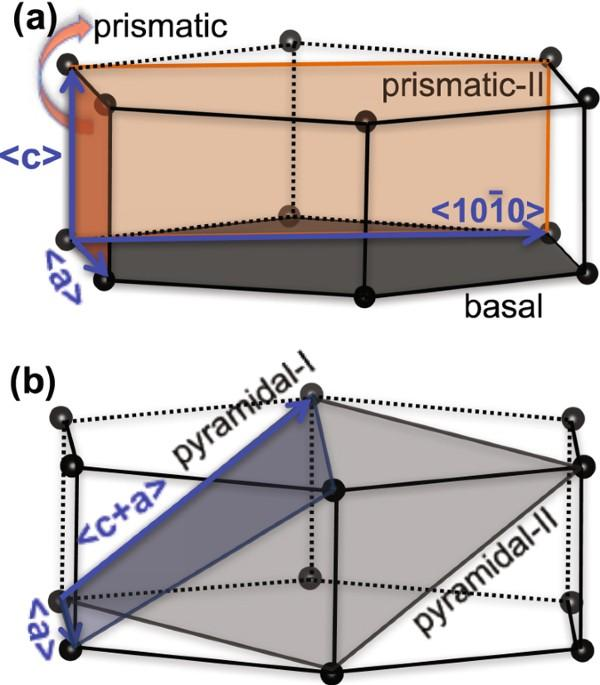
\includegraphics[width=0.52\textwidth]{HCP_crystal.png}
\caption{The principal planes and lattice translations of the hcp structure, on
which the nine families of \cref{eq:families} are placed. (a)~The families
whose normals are perpendicular or parallel to $[0001]$: the \emph{basal} plane
$(0001)$ (shaded, bottom), which is the habit of $c_0$, $c_f$ and $c_p$; the
first-order \emph{prismatic} plane $\{10\bar10\}$, a side face of the prism (the
narrow shaded face at the left, indicated by the curved arrow), which is the
habit of $a_1,a_2,a_3$; and the second-order \emph{prismatic-II} plane
$\{11\bar20\}$, a diagonal plane through the cell rather than a face of it (the
wide shaded region), on which \aloop{} loops are also observed. The blue arrows
are the two shortest lattice translations,
$\langle a\rangle=\tfrac13\langle11\bar20\rangle$ in the basal plane and
$\langle c\rangle=[0001]$ along the cell axis. (b)~The inclined
\emph{pyramidal-I} $\{10\bar11\}$ and \emph{pyramidal-II} $\{11\bar22\}$ planes,
which contain $\langle c+a\rangle=\tfrac13\langle11\bar23\rangle$ and which
carry \emph{no} family of \cref{eq:families}. The cell is drawn at an arbitrary
axial ratio, whereas $\alpha$-Zr has $c/a\simeq1.5944$ (\cref{eq:lattice}).}
\label{fig:hcp-cell}
\end{figure}

Two readings of the figure guard against errors the family set would otherwise
invite. First, $\langle c+a\rangle$ in panel~(b) is close in magnitude to the
basal Burgers vectors of \cref{eq:c2,eq:c2p} but is a different vector of
different character --- it is the glide vector that accommodates $c$-axis strain
in deformation --- and the pyramidal planes containing it are not observed habit
planes for irradiation-induced loops. \Cref{eq:families} therefore has no
pyramidal family, and that is an experimental statement rather than a
truncation. Second, the two habits are mutually \emph{orthogonal}: the normals
$\hat{\bm a}_k$ of the three prismatic variants lie in $(0001)$, while the basal
normal is $[0001]$ itself. That orthogonality is why no single electron-beam
direction images both populations at true size --- a zone axis showing one
family face-on views the other edge-on --- so any comparison of
\cref{eq:families} against TEM densities must combine at least two zone axes,
and a single-axis micrograph constrains at most one habit.

The quantity converting loop area into stored defects is not $|\bvec|$ but the
edge component $\bvec\!\cdot\!\nvec$: a loop of radius $R$ holds $\pi
R^2(\bvec\!\cdot\!\nvec)/\Omega$ defects. The mean radius and the line density of
family $(s,k)$ therefore follow from its content and density as
\begin{equation}
  R^k_{sL}=\lambda_k\sqrt{\frac{c^k_{sL}}{n^k_{sL}}},
  \qquad
  \lambda_k=\sqrt{\frac{\Omega}{\pi\,(\bvec\!\cdot\!\nvec)_k}},
  \qquad
  \rho^k_{sL}=2\pi R^k_{sL}\,n^k_{sL},
  \label{eq:radius}
\end{equation}
with one geometric length per habit --- $\lambda_a$ shared by all six prismatic
families, $\lambda_{c_f}$ and $\lambda_{c_p}$ for the two basal states --- and
the mean number of defects per loop is $m^k_{sL}=c^k_{sL}/n^k_{sL}$.
\Cref{tab:cd-families} lists the nine families with the crystallography that
fixes their geometry.
\Cref{eq:radius} describes a planar object and does not apply to the pyramid,
whose stored vacancies fill a volume rather than bound an area. Its size follows
instead from the volumetric relation already used for the compact limit in
\cref{eq:Rtransition},
\begin{equation}
  R^{c_0}_{vL}=\left(\frac{m^{c_0}_{vL}\,\Omega}{\sqrt8}\right)^{1/3},
  \qquad
  m^{c_0}_{vL}=\frac{c^{c_0}_{vL}}{n^{c_0}_{vL}},
  \label{eq:Rsfp}
\end{equation}
so the pyramid carries no $\lambda_k$, no Burgers vector and no line density.
What it does carry is a capture cross-section, and \cref{eq:Pi-identity} below
shows that a cross-section is the only thing either the growth law or the sink
strengths ever ask of a family.

\begin{table}[htbp]
\centering
\caption{The nine families of \cref{eq:families}; the first eight are
dislocation loops and $c_0$ is not. The three prismatic
variants are related by the sixfold symmetry of the $c$ axis and are
crystallographically equivalent at zero stress. $\lambda_k$ is evaluated with
$\Omega=2.3266\times10^{-29}\,$m$^3$, $a=0.323\,$nm, $c=0.515\,$nm.}
\label{tab:cd-families}
\begin{tabularx}{\textwidth}{@{}l l l c r X@{}}
\toprule
Family & Habit & $\bvec$ & Character & $\lambda_k$ (nm) & Comment \\
\midrule
$a_1,a_2,a_3$ & $\{10\bar10\}$ & $\tfrac13\langle11\bar20\rangle$ &
  $i$ & 0.151 & The dominant early population; $\bvec\!\cdot\!\nvec=a$. \\
$a_1,a_2,a_3$ & $\{10\bar10\}$ & $\tfrac13\langle11\bar20\rangle$ &
  $v$ & 0.151 & Same habit and $|\bvec|$ as the interstitial variants;
  separated from them only by capture character (\cref{sec:character}). \\
$c_f$ & $(0001)$ & $\tfrac16\langle20\bar23\rangle$ &
  $v$ & 0.170 & Faulted, $\bvec\!\cdot\!\nvec=c/2$, one removed basal layer.
  The dominant observed $c$ loop. \\
$c_p$ & $(0001)$ & $[0001]$ &
  $v$ & 0.120 & Perfect, $\bvec\!\cdot\!\nvec=c$, two removed layers, hence
  $\lambda_{c_p}=\lambda_{c_f}/\sqrt2$. \\
$c_0$ & $(0001)$ base & partials &
  $v$ & --- & The stacking-fault pyramid: not planar, so \cref{eq:radius} is
  replaced by \cref{eq:Rsfp} and it carries no $\lambda_k$. Precursor to $c_f$
  (\cref{sec:basal}). \\
\bottomrule
\end{tabularx}
\end{table}

\paragraph{The loops are elliptical; the model carries their equal-area radius.}
\Cref{eq:radius} treats every family as a circle. A real prismatic loop is not
one: its outline is an ellipse with the major axis close to $[0001]$ and the
minor axis the basal direction contained in the habit plane
(\cref{fig:loop-geometry}, left), and the ellipticity $e=1-d_{\min}/d_{\max}$
reaches $\simeq0.1$ for large interstitial and $\simeq0.4$ for large vacancy
\aloop{} loops, for the reasons given in \cref{sec:loopchar}. Three statements
bound what the circular idealization costs, and none of them touches
\cref{eq:growth}.

\begin{figure}[htbp]
\centering
\begin{minipage}[t]{0.49\textwidth}\centering
\adjustbox{max width=\linewidth}{%
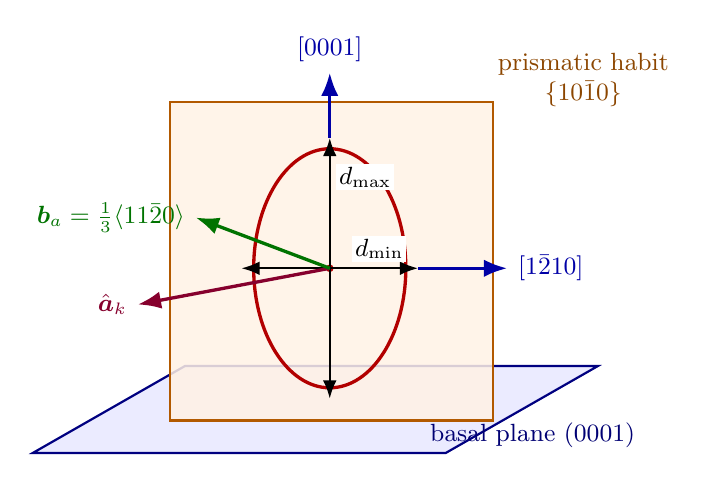
\begin{tikzpicture}[scale=0.92,>=Latex,font=\small]
  \fill[blue!8] (-4,-2.0) -- (1.7,-2.0) -- (3.8,-0.8) -- (-1.9,-0.8) -- cycle;
  \draw[blue!50!black,thick] (-4,-2.0) -- (1.7,-2.0) -- (3.8,-0.8) -- (-1.9,-0.8) -- cycle;
  \node[blue!45!black] at (2.9,-1.75) {basal plane $(0001)$};
  \fill[orange!10,opacity=.85] (-2.1,-1.55) -- (2.35,-1.55) -- (2.35,2.85) -- (-2.1,2.85) -- cycle;
  \draw[orange!70!black,thick] (-2.1,-1.55) rectangle (2.35,2.85);
  \node[orange!55!black,align=center] at (3.6,3.15) {prismatic habit\\$\{10\bar10\}$};
  \draw[very thick,red!70!black] (0.1,0.55) ellipse [x radius=1.05,y radius=1.65];
  \fill[red!70!black] (0.1,0.55) circle (1.5pt);
  \draw[<->,thick] (0.1,-1.25) -- (0.1,2.35)
    node[pos=0.85,right=2pt,fill=white,inner sep=1pt] {$d_{\max}$};
  \draw[<->,thick] (-1.12,0.55) -- (1.32,0.55)
    node[pos=0.78,above=2pt,fill=white,inner sep=1pt] {$d_{\min}$};
  \draw[->,very thick,blue!65!black] (0.1,2.35) -- (0.1,3.25) node[above] {$[0001]$};
  \draw[->,very thick,blue!65!black] (1.32,0.55) -- (2.55,0.55)
    node[right] {$[1\bar210]$};
  \draw[->,very thick,purple!70!black] (0.1,0.55) -- (-2.55,0.05)
    node[left,align=right] {$\hat{\bm a}_k$};
  \draw[->,very thick,green!45!black] (0.1,0.55) -- (-1.75,1.25)
    node[left,align=right] {$\bvec_a=\tfrac13\langle11\bar20\rangle$};
\end{tikzpicture}}
\end{minipage}\hfill
\begin{minipage}[t]{0.49\textwidth}\centering
\adjustbox{max width=\linewidth}{%
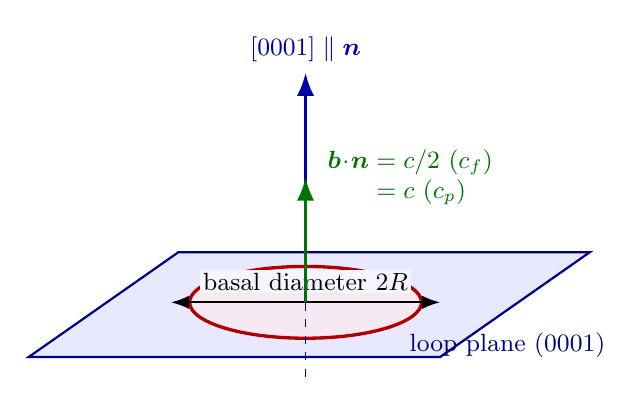
\begin{tikzpicture}[scale=0.95,>=Latex,font=\small]
  \fill[blue!9] (-3.7,-1.35) -- (1.8,-1.35) -- (3.8,0.05) -- (-1.7,0.05) -- cycle;
  \draw[blue!55!black,thick] (-3.7,-1.35) -- (1.8,-1.35) -- (3.8,0.05) -- (-1.7,0.05) -- cycle;
  \fill[red!8,opacity=.65] (0,-0.62) ellipse [x radius=1.55,y radius=.48];
  \draw[very thick,red!70!black] (0,-0.62) ellipse [x radius=1.55,y radius=.48];
  \draw[<->,thick] (-1.8,-0.62)--(1.8,-0.62)
    node[midway,above=3pt,fill=blue!4,inner sep=1pt] {basal diameter $2R$};
  \draw[->,very thick,blue!65!black] (0,-0.62)--(0,2.45)
    node[above] {$[0001]\parallel\nvec$};
  \draw[dashed,blue!65!black] (0,-0.62)--(0,-1.65);
  \draw[->,very thick,green!45!black] (0,-0.62)--(0,1.05)
    node[right=4pt,align=left] {$\bvec\!\cdot\!\nvec=c/2$ ($c_f$)\\
                                $\phantom{\bvec\!\cdot\!\nvec}=c$ ($c_p$)};
  \node[blue!50!black] at (2.7,-1.2) {loop plane $(0001)$};
\end{tikzpicture}}
\end{minipage}
\caption{Geometry of the two habits of \cref{eq:families}; both drawings are
schematic in perspective rather than metrically crystallographic. \emph{Left:} a
prismatic \aloop{} family $a_k$. The loop plane contains $[0001]$ and one basal
$a$ direction, the outline is elongated along $[0001]$, and the Burgers vector
is basal while the measured habit normal $\hat{\bm a}_k$ --- the vector on which
\cref{eq:variant-weight,eq:Zsk} resolve the stress --- need not be exactly
parallel to it. \emph{Right:} a basal family $c_f$ or $c_p$. The closed line and
both shape axes lie in $(0001)$ and $[0001]$ is the loop \emph{normal}; the
apparent ellipse is the oblique projection of a circular basal loop and must not
be read as intrinsic ellipticity. For $c_f$ the Burgers vector additionally
carries the basal partial of \cref{eq:unfault-partial}, so it is
$\bvec\!\cdot\!\nvec$, and not $|\bvec|$, that appears in \cref{eq:radius}.}
\label{fig:loop-geometry}
\end{figure}

\begin{enumerate}
\item \textbf{The stored content is exact.} $R^k_{sL}$ in \cref{eq:radius} is
      defined through the loop \emph{area}, $\pi R^2=\tfrac{\pi}{4}d_{\max}
      d_{\min}$, so $c^k_{sL}$ and $m^k_{sL}=c^k_{sL}/n^k_{sL}$ are independent
      of the outline shape. Ellipticity redistributes a loop's perimeter; it
      does not change how many defects a loop of given area stores.
\item \textbf{Only the line density is affected, and by at most $5\%$.} The
      perimeter of an ellipse exceeds that of the circle of equal area, so
      $\rho^k_{sL}=2\pi R^k_{sL}n^k_{sL}$ understates the true line length by a
      factor
      \begin{equation}
        \frac{P}{2\pi R}=\frac{2}{\pi\sqrt{q}}\,E\!\left(1-q^{2}\right),
        \qquad q=\frac{d_{\min}}{d_{\max}}=1-e,
        \label{eq:ellip-perimeter}
      \end{equation}
      with $E$ the complete elliptic integral of the second kind. This is
      $1.0021$ at $e=0.1$ and $1.0490$ at $e=0.4$: the interstitial \aloop{}
      families are circular to two parts in a thousand, and even the most
      elliptical vacancy \aloop{} loops carry $4.9\%$ more line than
      \cref{eq:radius} credits them with. That is the single place shape enters
      the formulation, and it is an order of magnitude below the spread on the
      capture efficiencies it would multiply.
\item \textbf{The stress response and the basal families are untouched.} The
      habit normal $\hat{\bm a}_k$ on which \cref{eq:variant-weight,eq:Zsk}
      resolve the stress is a property of the habit \emph{plane}, not of the
      outline drawn in it, so SIPN and SIPA are independent of $e$. And for
      $c_f$ and $c_p$ the equal-area circle is not an idealization at all to
      within the sixfold basal symmetry: $[0001]$ is their normal rather than an
      in-plane axis, so an isolated basal loop has no preferred in-plane
      direction to elongate along (\cref{fig:loop-geometry}, right).
\end{enumerate}

What the family set does not carry is the ellipticity itself, and in particular
its \emph{divergence} between the two characters. That divergence is driven by
the same anisotropy parameters $p^m$ that generate the orientation factors
$A_{h(k)}(p^m)$ of \cref{eq:Afactors}, so a shape-resolved extension would be a
second use of a quantity already in the model rather than a new mechanism: it
would enter as one aspect ratio per family multiplying $\rho^k_{sL}$, and by
item~2 it could move the sink strengths of \cref{eq:KL_matrix} by no more than
$5\%$. The expansion that matters for the coexistence problem is the one
\cref{eq:families} makes --- resolving the variants and the characters --- not
the shape of the individual loop.

\subsection{Capture efficiencies: orientation, character, and stress}
\label{sec:character}

Every efficiency in the model is built as a product of three factors, one per
degeneracy to be broken:
\begin{equation}
  Z_{sk,m}(\bm\sigma)
  =\underbrace{Z^0_m}_{\text{elastic bias}}\;
   \underbrace{A_{h(k)}(p^m)}_{\text{DAD, orientation}}\;
   \underbrace{X_{s,m}}_{\text{character}}\;
   \underbrace{\left[1+\frac{\Delta Z^{\mathrm{SIPA}}_{h(k),m}(\sigma_{kk})}
                          {Z^0_m A_{h(k)}(p^m)}\right]}_{\text{stress, SIPA}},
  \label{eq:Zsk}
\end{equation}
where $h(k)\in\{a,c\}$ is the habit of family $k$ and
\begin{equation}
  A_a(p)=\frac{p+p^{-2}}{2},\qquad A_c(p)=p .
  \label{eq:Afactors}
\end{equation}
Each factor breaks exactly one degeneracy, and each is silent on the others.

\begin{itemize}
\item $A_{h(k)}(p^m)$ is the Woo DAD factor \cref{eq:Zdad}. It depends on the
      habit plane alone, through the angle between the loop normal and the $c$
      axis, and therefore assigns one pair to all six prismatic families and one
      pair to all three basal states, the pyramid included, whose base is
      $(0001)$ so that $h(c_0)=c$. It separates prismatic from basal --- opening
      the window \cref{eq:window} --- and it separates nothing else.
\item $X_{s,m}$ is the character factor. It is unity in the
      character-degenerate model, and $X_{i,I},X_{v,V}>X_{i,V},X_{v,I}$ when the
      thermal-drift capture radii of \cref{eq:zST} are used, so that
      \begin{equation}
        \chi=\frac{X_{i,I}X_{v,V}}{X_{i,V}X_{v,I}}>1
        \label{eq:chi-from-X}
      \end{equation}
      and the prismatic window acquires the finite logarithmic width $\ln\chi$
      of \cref{eq:chi}. It is the same for the three variants of a given
      character, since \cref{eq:chi} resolves character and not orientation.
      \textbf{$\chi=1$ recovers the character-degenerate model exactly, which is
      the regression test on this factor.} Note the double-counting hazard of
      \cref{sec:coexist}: $X_{s,m}$ and $Z^0_m$ describe overlapping elastic
      physics, so only one of them may carry the interstitial--vacancy
      asymmetry. The clean choice is to take $X_{s,m}$ from the capture radii
      and set $Z^0_m$ to unity; if $Z^0_m$ is retained as a fitting parameter, it
      must be stated that it absorbs whatever the capture-radius database does
      not.
\item The SIPA bracket carries the applied stress, resolved on each family's own
      habit plane through $\sigma_{kk}=\hat{\bm a}_k\cdot\bm\sigma\cdot\hat{\bm
      a}_k$ for the prismatic variants and $\sigma_{33}$ on $(0001)$ for the
      basal pair. It separates $a_1$ from $a_2$ from $a_3$, which nothing else
      in \cref{eq:Zsk} can do. At $\bm\sigma=\bm0$ the bracket is unity and every
      efficiency reduces to its DAD value.
\end{itemize}

\Cref{eq:Zsk} is the whole of the self-consistency claim in one equation. Its
$p^m$ is the anisotropy of the very tensor $\bm D^m$ that transports species $m$
in \cref{Eq:master_c}; its $\overline{D}^m$, used in \cref{eq:growth}, is that
tensor's orientation average; and the same $Z_{sk,m}$ appears in the sink
strengths \cref{eq:KL_matrix} that debit the mobile species. One set of
transport parameters, one set of efficiencies, both sides of the coupling.

\subsection{Growth of the stored content}
\label{sec:growth-laws}

Loop growth is the rate of change of stored content under the net biased flux of
the correct sign for the family. All nine families obey one law,
\begin{equation}
  \left.\dot c^k_{sL}\right|_{\mathrm{growth}}
  =\underbrace{\Pi^k_{sL}}_{\text{geometry}}\;\eta_s
   \sum_{m\in\{v,i,2i,3i\}}\!\!
   |m|\;\overline{D}^m\,Z_{sk,m}\,c^m\;\varsigma_{s}(m)\;g^k_{sL},
  \label{eq:growth}
\end{equation}
with $\varsigma_s(m)=+1$ when the polarity of species $m$ matches the character
$s$ and $-1$ otherwise, $|m|$ the number of point defects the mobile cluster
carries, and
\begin{equation}
  \Pi^k_{sL}=\frac{\lambda_k}{\ell}\;\varsigma^{\mathrm{sink}}_k\,
             \sqrt{n^k_{sL}\,c^k_{sL}},
  \qquad
  \ell\equiv\frac{z_c\Omega}{2\pi a^2},
  \label{eq:loopprefactor}
\end{equation}
the loop-perimeter prefactor implied by \cref{eq:radius}, in which
$\varsigma^{\mathrm{sink}}_k$ is the per-family sink-scale calibration constant.
\Cref{eq:loopprefactor} is a special case of a more general statement, and
writing that statement out is what carries \cref{eq:growth} onto the pyramid
unchanged. Because $\rho^k_{sL}=2\pi R^k_{sL}n^k_{sL}
=2\pi\lambda_k\sqrt{n^k_{sL}c^k_{sL}}$ by \cref{eq:radius},
\begin{equation}
  \Pi^k_{sL}=\varsigma^{\mathrm{sink}}_k\,\frac{\rho^k_{sL}}{2\pi\ell}
  \qquad\text{identically, for every }(s,k)\in\mathcal F_L,
  \label{eq:Pi-identity}
\end{equation}
that is, \emph{the prefactor in the growth law is the family's own sink density
divided by $2\pi\ell$}. A family therefore needs no geometry beyond the capture
cross-section it presents to the mobile species, and the pyramid --- which has no
perimeter --- supplies that cross-section in the compact form of
\cref{eq:partial_sink_bp}:
\begin{equation}
  \Pi^{c_0}_{vL}
  =\varsigma^{\mathrm{sink}}_{c_0}\,
    \frac{\alpha_{\mathrm{sfp}}\,\pi R^{c_0}_{vL}\,n^{c_0}_{vL}}{2\pi\ell}
  =\varsigma^{\mathrm{sink}}_{c_0}\,
    \frac{\alpha_{\mathrm{sfp}}\,R^{c_0}_{vL}\,n^{c_0}_{vL}}{2\ell},
  \label{eq:Pisfp}
\end{equation}
with $R^{c_0}_{vL}$ from \cref{eq:Rsfp} and $\alpha_{\mathrm{sfp}}$ the pyramid
capture prefactor of \cref{eq:partial_sink_bp}. With \cref{eq:Pisfp} substituted
for \cref{eq:loopprefactor}, all nine families obey \cref{eq:growth} in one form,
and \cref{eq:Pi-identity} guarantees in advance what \cref{sec:conservation} has
to verify: what a family absorbs in \cref{eq:growth} is exactly what it debits
from the mobile pool in \cref{eq:KL_matrix}, the pyramid included.
The gate $g^k_{sL}\in[0,1]$ is applied to the \emph{shrinking} channel only and
suppresses it as $R^k_{sL}\to R^k_{\min}$,
\begin{equation}
  g(R)=\begin{cases}0,& u\le0,\\ u^2(3-2u),&0<u<1,\\ 1,& u\ge1,\end{cases}
  \qquad u=\frac{R/R_{\min}-1}{w_R},
  \label{eq:gate}
\end{equation}
a $C^1$-continuous smoothstep chosen to avoid solver stiffness. Gating the whole
opposite-polarity absorption term, rather than the net rate, keeps the
point-defect balance closed: the un-absorbed defects stay in the free pool.
\Cref{eq:gate} is a device for keeping a \emph{mean} size off a floor that a
single size cannot cross, and \cref{sec:moments} retires it: once the family
carries a distribution, loops leave through the floor at the rate
\cref{eq:floorcurrent} determines, and there is nothing left for a smoothstep to
prevent.

Two things about \cref{eq:growth} are worth isolating.

\paragraph{It is species-resolved, not flux-lumped.} The sum runs over the four
mobile species with each carrying its own $\overline{D}^m$ and its own
$Z_{sk,m}$. Writing it instead as $\Pi(Z_{s,I}\Phi_I-Z_{s,V}\Phi_V)$ with the
aggregates \cref{eq:flux} is the mean-field reduction, and it is lossy in a way
that matters here: an anisotropy assigned to the clusters alone is invisible to
it. In the present parameter set the di- and tri-interstitials carry $3.1\%$ of
the interstitial arrival, so the difference is small at these parameters and
structural in general.

\paragraph{Loop growth is a near-cancellation.} \Cref{eq:growth} is the small
residual of two much larger opposing fluxes, and this is the single most
important numerical property of the immobile block. Measured on a prismatic
interstitial family at $10\,$dpa, the interstitial gain and the vacancy loss
agree to within a few percent, so the net content rate is a few percent of
either. Small changes in a capture efficiency therefore produce large changes in
net growth --- which is exactly what makes the window analysis of
\cref{sec:coexist} predictive, and equally what makes any parameter set fitted
against one formulation stale for another.

Collecting the families, the debits on the mobile pool are the sums of the
same species-resolved terms with the opposite sign,
\begin{equation}
  \mathrm{loop\_abs}_m=\sum_{(s,k)\in\mathcal F}
    \Pi^k_{sL}\,|m|\,\overline{D}^m\,Z_{sk,m}\,c^m\,g^k_{sL},
  \qquad
  \mathrm{loop\_recomb}=\!\!\sum_{(s,k)\in\mathcal F}\!\!
    \Bigl[\text{opposite-polarity terms}\Bigr],
  \label{eq:loopabs}
\end{equation}
which enter \cref{Eq:master_c} through $\spmat{D}\spvec{c}_M$. Every defect
debited from the mobile pool by \cref{eq:loopabs} is credited to a family by
\cref{eq:growth}, term by term, so nothing is double-counted and nothing is
lost.

\subsection{Variant resolution and where the stress enters}
\label{sec:stress}

The three prismatic variants are crystallographically equivalent about the $c$
axis, so nothing in \cref{eq:Afactors} separates them and an unstressed grain has
no reason to prefer one. A stress does, and it acts in two places, both of them
Boltzmann factors of the work the stress does on the defect volume the loop
stores.

\paragraph{Partition of the sources.} Production into variant $k$ is weighted by
the resolved normal stress on its habit plane and by the sign of the relaxation
volume the loop carries, so that interstitial and vacancy loops of one variant
respond in \emph{opposite} senses:
\begin{equation}
  w^s_k(\bm\sigma,T)
  =\frac{\exp\!\bigl(\eta_s\,\sigma_{kk}V_s/k_BT\bigr)}
        {\sum_{k'=1}^{3}\exp\!\bigl(\eta_s\,\sigma_{k'k'}V_s/k_BT\bigr)},
  \qquad \sum_{k=1}^{3}w^s_k=1,
  \qquad s\in\{i,v\},
  \label{eq:variant-weight}
\end{equation}
with $V_s$ the formation (relaxation) volume of the clustering unit. A tensile
normal stress on the habit plane favors interstitial loops of that variant and
disfavors vacancy loops of it, which is stress-induced preferential nucleation
(SIPN) in its simplest form. \Cref{eq:variant-weight} is the
scalar-activation-volume case of the general partition through the
formation-volume tensor $\bm\Omega^k$,
\begin{equation}
  \chi^k_s=\frac{\exp\!\left(\bm\sigma:\bm\Omega^k/k_BT\right)\mathcal I^k_s}
                {\sum_p\exp\!\left(\bm\sigma:\bm\Omega^p/k_BT\right)\mathcal I^p_s},
  \label{eq:SIPN}
\end{equation}
in which $\sigma_{kk}V_s$ is replaced by $\bm\sigma\!:\!\bm\Omega^k$ and
$\mathcal I^k_s$ is the character selector. At zero deviatoric stress
$w^s_k=\tfrac13$ for every variant and every character, and
\cref{eq:variant-weight} replaces the scalar alignment fraction $f_a$ of the
lumped model entirely. Linearizing \cref{eq:variant-weight} for small stress
gives $w^s_k\simeq\tfrac13(1+\eta_s\varsigma\,\hat\sigma_{kk})$, which is the
form the code carries.

\paragraph{Stress in the growth law.} The same work term enters the vacancy
concentration a loop is in equilibrium with, and hence the emission side of
\cref{eq:growth} and the annealing lifetime, through
$C_v^{\mathrm{eq}}(k)\propto\exp(+\sigma_{kk}\Omega/k_BT)$. This is the
channel by which a variant under an unfavorable stress \emph{shrinks} rather
than merely being nucleated less often, and it is the one that produces
irradiation creep at constant loop number. It acts in the same direction as
\cref{eq:variant-weight}, so the two contributions to the variant imbalance add.

Because all three basal states share a single habit plane, no such partition
applies to them: a stress acts on $c_0$, $c_f$ and $c_p$ only through the second
channel, with $\sigma_{33}$ resolved on $(0001)$. \textbf{That asymmetry --- three
prismatic variants that redistribute, one basal orientation that cannot --- is
the origin of the texture dependence of irradiation growth}, and it is not
representable at all in a model whose stress dependence is a single scalar
alignment fraction.

\subsection{The basal chain: pyramid, faulted loop, perfect loop}
\label{sec:basal}

\Cref{sec:loopchar} established the crystallography of the chain
\cref{eq:basal-chain}; this subsection gives its kinetics. Four properties fix
how the triple $(c_0,c_f,c_p)$ is treated, and the fourth is the one that makes
the chain more than a relabelling.

\begin{enumerate}
\item \textbf{Only $c_0$ is nucleated.} Cascade collapse on basal planes produces
      pyramids, not loops. The faulted state is reached only through the collapse
      transition below and the perfect state only through unfaulting, so
      $J^{c_f}_{vL}=J^{c_p}_{vL}=0$ in the pure-precursor limit. A direct basal
      loop current $J^{c_f}_{vL}$ is retained as an option in
      \cref{eq:nucleation} because setting $\varepsilon_{\mathrm{sfp}}=0$ and
      restoring it recovers the previous revision of the model exactly, which is
      the regression test on this addition.
\item \textbf{The planar states store different content per unit area.} A $c_p$
      loop removes two basal layers where a $c_f$ loop removes one, so
      $(\bvec\!\cdot\!\nvec)_{c_p}=2(\bvec\!\cdot\!\nvec)_{c_f}$ and
      $\lambda_{c_p}=\lambda_{c_f}/\sqrt2$ in \cref{eq:radius}. Two loops of equal
      radius differ by a factor of two in stored vacancies, which is why the two
      cannot be lumped even though they share a habit plane. Because $c_f$ is not
      a pure edge loop --- its Burgers vector contains the basal partial of
      \cref{eq:unfault-partial} --- it is the edge component
      $\bvec\!\cdot\!\nvec=c/2$, and not $|\tfrac16\langle20\bar23\rangle|$, that
      enters its content.
\item \textbf{All three share their capture efficiencies.} The pyramid's base and
      both loop habits are $(0001)$, so \cref{eq:Zsk} assigns $h(c_0)=h(c_f)
      =h(c_p)=c$ and all three take $A_c(p^m)$, the same character factor
      $X_{v,m}$ and the same resolved stress $\sigma_{33}$. They are three states
      of one population, not three competing sinks in the sense that the
      prismatic variants are. What differs among them is not $Z$ but the
      cross-section that multiplies it --- \cref{eq:Pisfp} for the pyramid,
      \cref{eq:loopprefactor} for the loops.
\item \textbf{Only the planar states carry $c$-axis eigenstrain.} The pyramid's
      relaxation volume is nearly isotropic, \cref{eq:Omegatransition} with
      $\bm\Omega_{\mathrm{pyr}}=\mathcal I\,\mathbb I V/3$, so vacancies held in
      $c_0$ contribute to the hydrostatic part of the eigenstrain and only
      $\zeta_{c_0}\simeq\tfrac13$ of their share to $\varepsilon_c$
      (\cref{eq:strain}). Storing a vacancy in a pyramid is therefore \emph{not}
      equivalent to storing it in a loop, and this is the property that turns the
      residence time in $c_0$ into an incubation period for $c$-axis growth.
\end{enumerate}

\paragraph{The two transitions.} Both are one-way, thermally activated, and
size-gated: a cluster converts once it is large enough for the destination state
to be the lower-energy one (\cref{eq:sfp-competition} for the first,
\cref{eq:fault-competition} for the second) and once it has waited long enough to
cross the barrier. Writing $\theta\in\{\mathrm{col},\mathrm{uf}\}$ for the two,
\begin{equation}
  \nu_\theta(T)=\nu^0_\theta\exp\!\left(-\frac{E_\theta}{k_BT}\right),
  \qquad
  \Phi^{(j)}_\theta=\frac{1}{\langle m^j\rangle_k}
     \int_{R_\theta}^{\infty}\!\!m^{j}f_k(R)\,\mathrm dR ,
  \label{eq:barrier}
\end{equation}
in which $E_{\mathrm{col}}$ is the pyramid-to-loop collapse barrier,
$E_{\mathrm{uf}}$ the unfaulting barrier, $R_{\mathrm{col}}$ and
$R_{\mathrm{uf}}$ the critical radii implied by \cref{eq:sfp-competition,%
eq:fault-competition}, and $f_k(R)$ the size distribution of the source family
--- \emph{not} an assumed one: \cref{sec:moments} carries enough moments to
construct it, and \cref{eq:gatefraction} evaluates $\Phi^{(j)}_\theta$ in closed
form. \textbf{The gate must be a distribution fraction and not a Heaviside step
on the mean radius}: in a mean-field state $R^k_{vL}$ is an average, and a hard
threshold on an average transfers the entire family in one step. The three
weights are needed because a transfer moves number, content and second content
in different proportions --- the converting subpopulation is larger than the
family mean. Setting
$\Phi^{(j)}_\theta\equiv1$ makes a transition purely barrier-limited; setting
$\nu_\theta=0$ removes it, and $\nu_{\mathrm{col}}=0$ leaves the pyramids as a
terminal population while $\nu_{\mathrm{uf}}=0$ leaves the single basal loop
family the model carried before.

The transfers themselves are written so that both number and content move
together, with the \emph{same} rate multiplying each:
\begin{align}
  \Gamma^{n}_{\theta}&=\nu_\theta\,\Phi^{(0)}_\theta\,n^{k(\theta)}_{vL},
  &
  \Gamma^{c}_{\theta}&=\nu_\theta\,\Phi^{(1)}_\theta\,c^{k(\theta)}_{vL},
  &
  \Gamma^{q}_{\theta}&=\nu_\theta\,\Phi^{(2)}_\theta\,q^{k(\theta)}_{vL},
  \label{eq:transfer}
\end{align}
with source $k(\mathrm{col})=c_0$ and $k(\mathrm{uf})=c_f$. Whatever leaves one
family arrives in the other, moment for moment, so no vacancy is created or
destroyed by either step. Because $\Phi^{(2)}_\theta>\Phi^{(1)}_\theta>
\Phi^{(0)}_\theta$, the converting subpopulation is larger than the family mean:
a transfer therefore \emph{lowers} the mean size of the source and delivers to
the destination a population above the source mean, which is what a size-gated
reaction does and what a single rate multiplying every moment could not
express. For the unfaulting transfer that statement has a
geometric reading --- by \cref{eq:radius} the transferred loops arrive with their
radius reduced by $1/\sqrt2$, the same vacancies now occupying half the area on
two layers --- and for the collapse it has another: by \cref{eq:Rsfp} and
\cref{eq:radius} a pyramid of $m$ vacancies arrives as a faulted loop of radius
$\lambda_{c_f}\sqrt m$, which is larger than the pyramid it came from whenever
$m>(\Omega/\sqrt8)^{2}\lambda_{c_f}^{-6}$, so collapse is a spreading of the same
vacancies into a plane.

\paragraph{Saturation of the pyramid population, in closed form.} The pyramid has
no coalescence channel --- it is a compact cluster and not a line sink, and the
loop--loop and loop--network channels of \cref{eq:coal} are defined on
$\mathcal F_L$ --- so its density is controlled by exactly the two loss channels
of \cref{sec:number}: thermal dissolution at $1/\tau_{\mathrm{sfp}}$, and
conversion at $\nu_{\mathrm{col}}\Phi_{\mathrm{col}}$. Its number equation is
therefore linear in $n^{c_0}_{vL}$ and saturates at
\begin{equation}
  n^{c_0,\ast}_{vL}
  =\frac{J^{c_0}_{vL}}{\tau_{\mathrm{sfp}}^{-1}+\nu_{\mathrm{col}}\Phi_{\mathrm{col}}},
  \qquad
  f_{\mathrm{col}}
  =\frac{\nu_{\mathrm{col}}\Phi_{\mathrm{col}}}
        {\tau_{\mathrm{sfp}}^{-1}+\nu_{\mathrm{col}}\Phi_{\mathrm{col}}},
  \label{eq:sfp-saturation}
\end{equation}
where $f_{\mathrm{col}}$ is the branching ratio --- the fraction of pyramids that
become $c_f$ loops rather than dissolving back into the vacancy pool. It is
$f_{\mathrm{col}}$, and not $J^{c_0}_{vL}$, that is the \emph{effective} basal
loop nucleation efficiency of the model, and the two Arrhenius factors combine in
it into a single ratio,
\begin{equation}
  \nu_{\mathrm{col}}\tau_{\mathrm{sfp}}
  =\nu^0_{\mathrm{col}}\tau^0_{\mathrm{sfp}}
   \exp\!\left(\frac{E^{\mathrm{dis}}_{\mathrm{sfp}}-E_{\mathrm{col}}}{k_BT}\right),
  \label{eq:branching}
\end{equation}
so that $f_{\mathrm{col}}$ rises with temperature when
$E_{\mathrm{col}}>E^{\mathrm{dis}}_{\mathrm{sfp}}$ and falls when the inequality
reverses. That single sign is the model's prediction for the direction of the
temperature dependence of the $c$-loop onset dose, and it is a falsifiable
consequence of carrying the pyramid rather than nucleating $c_f$ directly: with
$\varepsilon_{\mathrm{sfp}}=0$ the onset dose has no barrier in it at all.

\subsection{The size distribution and its moments}
\label{sec:number}
\label{sec:moments}

A family in \cref{eq:families} is not a number of loops and a size. It is a
\emph{size distribution} $f_k(m,t)$, the density of loops of that family holding
between $m$ and $m+\mathrm dm$ defects, and everything the immobile block carries
is a moment of it. This subsection introduces the distribution first, because the
three fields the model advances are then one object seen three ways rather than
three separate balances that happen to be written together, and because the
closure that makes the third of them useful also makes the first two sharper.

\paragraph{From the master equation.} A loop does not change size continuously.
It changes by discrete events, each of which is the arrival of one mobile cluster
or the emission of one point defect, and the exact statement is therefore a
master equation on the integer size $m$ rather than a differential equation. Let
$W^{+}_{x}(m)$ be the rate at which a loop of size $m$ absorbs a mobile species
$x$ whose polarity \emph{matches} the family's character, and $W^{-}_{x}(m)$ the
rate for the opposite polarity; each event moves the loop by
\begin{equation}
  \mu_x=\left|m^x\right|\in\{1,2,3\},
  \label{eq:jump}
\end{equation}
the number of point defects the arriving cluster carries, from
\textttclr{mobileSpeciesVector}. Thermal emission is folded into $W^{-}$ with
$\mu=1$, since a loop emits one defect at a time. Then
\begin{equation}
\begin{split}
  \frac{\partial f_k(m,t)}{\partial t}
  =\sum_x\Bigl[&W^{+}_{x}(m-\mu_x)\,f_k(m-\mu_x)
              +W^{-}_{x}(m+\mu_x)\,f_k(m+\mu_x)\\
              &-\bigl(W^{+}_{x}(m)+W^{-}_{x}(m)\bigr)f_k(m)\Bigr]
  \;+\;J^k_{sL}\,\delta_{m,m^{\mathrm{nuc}}_k} ,
\end{split}
  \label{eq:master}
\end{equation}
a gain--loss balance in which the first two terms are loops arriving at $m$ from
below and from above and the third is loops leaving $m$ in either direction.
\textbf{\Cref{eq:master} is the exact statement}; \cref{eq:FP} is what it becomes
when the jumps are small.

The rates are not free. A loop captures on its perimeter, so $W^{\pm}_x\propto
R^k_{sL}=\lambda_k\sqrt m$, and the constant of proportionality is the same
capture efficiency and mobility that \cref{eq:growth} already carries:
\begin{equation}
  W^{\pm}_{x}(m)=\pi_k\sqrt m\;\overline D^{x}\,Z_{sk,x}\,c^{x},
  \qquad
  \pi_k=\frac{\lambda_k\,\varsigma^{\mathrm{sink}}_k}{\ell},
  \label{eq:Wrates}
\end{equation}
with the sign of the polarity match deciding whether a given $x$ enters $W^{+}$
or $W^{-}$. \textbf{No new parameter enters the size distribution.}

\paragraph{The Kramers--Moyal expansion.} Treat $m$ as continuous and expand the
shifted terms of \cref{eq:master} about $m$. The zeroth-order terms cancel the
loss term identically --- which is the statement that the process conserves loops
--- and what survives is
\begin{equation}
  \frac{\partial f_k}{\partial t}
   =\sum_{p\ge1}\frac{(-1)^{p}}{p!}\,
     \frac{\partial^{p}}{\partial m^{p}}\bigl[a_p(m)f_k\bigr]
   +J^k_{sL}\,\delta\!\left(m-m^{\mathrm{nuc}}_k\right),
  \qquad
  a_p=\sum_x\mu_x^{\,p}\Bigl[W^{+}_{x}+(-1)^{p}W^{-}_{x}\Bigr].
  \label{eq:KMexp}
\end{equation}
The first two coefficients are the physically familiar ones and they are
\emph{different combinations of the same rates}: $a_1$ is the difference of the
two directions and $a_2$ is their sum. \textbf{Truncating \cref{eq:KMexp} at $p=2$
is \cref{eq:FP}}, the Fokker--Planck equation for the size density,
\begin{equation}
  \frac{\partial f_k}{\partial t}
  =-\frac{\partial}{\partial m}\bigl[F_k f_k\bigr]
   +\frac{\partial^2}{\partial m^2}\bigl[D_k f_k\bigr]
   +J^k_{sL}\,\delta\!\left(m-m^{\mathrm{nuc}}_k\right),
  \label{eq:FP}
\end{equation}
in which the drift is the \emph{net} flux of \cref{eq:growth,eq:loopemission}
and the diffusion is half the \emph{gross} traffic across the same perimeter,
\begin{equation}
  F_k=a_1=\pi_k\sqrt m\,\Sigma^{\mathrm{net}}_k,
  \qquad
  D_k=\tfrac12 a_2=\tfrac12\,\pi_k\sqrt m\,\Sigma^{\mathrm{gro}}_k,
  \label{eq:FPcoeffs}
\end{equation}
\begin{equation}
  \Sigma^{\mathrm{net}}_k=\sum_x\varsigma_s(x)\,\mu_x\,\overline D^{x}Z_{sk,x}c^{x},
  \qquad
  \Sigma^{\mathrm{gro}}_k=\sum_x\mu_x^{2}\,\overline D^{x}Z_{sk,x}c^{x}.
  \label{eq:Sigmas}
\end{equation}
$\Sigma^{\mathrm{net}}_k$ is exactly the signed sum that multiplies $\Pi^k_{sL}$
in \cref{eq:growth}, so the drift of \cref{eq:FP} \emph{is} the growth law and
carries no independent content.

\textbf{Note the weighting in $\Sigma^{\mathrm{gro}}_k$.} It is not the net sum
with the signs made positive: the second Kramers--Moyal coefficient weights each
channel by $\mu_x^{2}$, one power more than the drift, because variance
accumulates as the square of the step. For the monomer channels, which carry
$\mu=1$, the two weightings coincide and the distinction is invisible --- and an
earlier revision of this document asserted on that basis that ``every absorption
and every emission is a $\pm1$ step''. That is true of $v$, $i$ and of emission
and false of $2i$ and $3i$. Those clusters carry $3.1\%$ of the interstitial
arrival in $\Sigma^{\mathrm{net}}_k$, so the extra power of $\mu_x$ raises their
share of $\Sigma^{\mathrm{gro}}_k$ to between $6\%$ and $9\%$: \textbf{the
spreading is under-estimated by $3$--$6\%$ if the drift weighting is used for
both}. Small, systematic, and in the direction that matters, since
\cref{eq:DoverF} is an argument that the spreading dominates.

\paragraph{Why truncating at second order is justified.} \Cref{eq:KMexp} is an
infinite series and \cref{eq:FP} keeps two terms of it. The expansion parameter
is \emph{not} the jump size itself but the jump size measured against the scale
over which $f_k$ varies: successive terms carry one more power of
$\mu_x\,\partial_m$, so
\begin{equation}
  \frac{\text{term }p+1}{\text{term }p}\;\sim\;\frac{\mu_x}{\sigma_m},
  \qquad
  \sigma_m^{2}=\int (m-\bar m^k_{sL})^{2}f_k\,\mathrm dm
             =\bigl(\bar m^k_{sL}\bigr)^{2}\bigl(\Delta_k-1\bigr),
  \label{eq:KMsmall}
\end{equation}
with $\sigma_m$ the width of the distribution. Three statements make this small
here, and they are worth separating because only the first is about the
absorption step alone.

\begin{enumerate}
\item \textbf{The step is small against the loop.} The mobile species are $v$,
      $i$, $2i$, $3i$, so $\mu_x\le3$ --- and \emph{this is a property of the
      species set, not an approximation}: there is no channel in this model that
      adds a large piece to a loop in one event. Against the sizes the families
      actually reach, measured on the reference march (interior medians, in
      defects per loop):
      \begin{center}\small
      \begin{tabular}{@{}lrrrr@{}}
      \toprule
      dose [dpa] & $\bar m_{\cloop{}}$ & $\mu_{\max}/\bar m_{\cloop{}}$
                 & $\bar m_{\aloop{}}$ & $\mu_{\max}/\bar m_{\aloop{}}$\\
      \midrule
      $10^{-4}$ & $584$ & $5.1\times10^{-3}$ & $294$ & $1.0\times10^{-2}$\\
      $0.1$ & $4.0\times10^{4}$ & $7.4\times10^{-5}$ & $183$ & $1.6\times10^{-2}$\\
      $10$ & $1.7\times10^{5}$ & $1.7\times10^{-5}$ & $695$ & $4.3\times10^{-3}$\\
      \bottomrule
      \end{tabular}
      \end{center}
      The worst case in the whole table is $1.6\times10^{-2}$, and the \aloop{}
      value at $10^{-4}\,$dpa is $294$ against a nucleus of
      $n^{\mathrm{nuc}}_{iL}=300$ --- the family has barely left its birth size,
      which is where this ratio is largest by construction.
\item \textbf{The rates vary slowly over a step.} \Cref{eq:KMexp} also requires
      $W^{\pm}_x(m\pm\mu_x)\simeq W^{\pm}_x(m)$ to the order retained. By
      \cref{eq:Wrates} the rates go as $\sqrt m$, so the relative change over one
      event is $\mu_x/2m$ --- the same smallness again, and \emph{half} it. A
      rate that varied exponentially in $m$ would not permit this truncation
      however small the step.
\item \textbf{The distribution is broad in units of the step.} This is the
      condition \cref{eq:KMsmall} actually names, and it is the one that can fail
      while the other two hold. Writing $N_{\mathrm{ex}}$ for the number of
      exchange events a loop has made, a random walk of step $\mu$ gives
      $\sigma_m=\mu\sqrt{N_{\mathrm{ex}}}$, so
      \begin{equation}
        \frac{\mu}{\sigma_m}=\frac{1}{\sqrt{N_{\mathrm{ex}}}},
        \qquad
        N_{\mathrm{ex}}=\frac{2}{\mu^{2}}\,\frac{D_k}{F_k}\,\Delta m ,
        \label{eq:Nex}
      \end{equation}
      the second form following from $\sigma_m^{2}=2D_kt$ and $\Delta m=F_kt$.
      \textbf{This is where \cref{eq:DoverF} does double duty.} The same
      near-cancellation that makes the second moment necessary --- $D_k/F_k$ of
      $7.3$ to $44$ --- also multiplies the number of exchanges a loop has made
      for a given net growth. With $D_k/F_k=44$ and the \cloop{} growth of the
      table above, $N_{\mathrm{ex}}\simeq1.5\times10^{7}$ and
      $\mu/\sigma_m\simeq2.6\times10^{-4}$; for \aloop{}, which grows by only a
      few hundred defects, $N_{\mathrm{ex}}\simeq3.5\times10^{4}$ and
      $\mu/\sigma_m\simeq5\times10^{-3}$.
\end{enumerate}

\textbf{Where the truncation is at its worst, and why it does not matter.}
\Cref{eq:Nex} diverges at $N_{\mathrm{ex}}=0$: a loop that has just nucleated has
made no exchanges, its distribution is a delta function, and no gradient
expansion describes it. The model injects exactly that, $J^k_{sL}\delta(m-
m^{\mathrm{nuc}}_k)$. The defect is real and it is bounded: it is confined to a
region of width $\sim\mu_x$ around $m^{\mathrm{nuc}}_k$, which is $1\%$ of the
nucleus, and it is cured by the first few exchange events, which at these fluxes
are immediate. \textbf{The second place the expansion is worst is the floor}
$m_{\min}$, where $f_k$ is cut off and its gradient is largest, and the model
does not rely on \cref{eq:FP} there at all --- \cref{eq:floorcurrent} carries an
explicit floor current instead, for exactly this reason.

\textbf{What the truncation is not.} It is not an assumption that the
distribution is Gaussian, or narrow, or near equilibrium; \cref{eq:FP} is solved
in moments and the closure of \cref{eq:closure} is a separate and later choice.
And it is not a statement about the channels \cref{eq:FP} omits: coalescence
removes whole loops rather than moving them along $m$, so it is not a jump
process in size at all and appears in \cref{eq:coal} instead --- which is also
why $\phi_{LL}$ and $\phi_{LN}$ carry their own validity criterion in
\cref{sec:dcoarsen} rather than inheriting this one.

\paragraph{Why the second moment is not a refinement here.} The two large
opposing fluxes that \emph{cancel} in $F_k$ \emph{add} in $D_k$, and
\cref{sec:growth-laws} has already established that this cancellation is severe.
Taking the measured
prismatic fluxes at $10\,$dpa:
\begin{equation}
  \frac{D_k}{F_k}
  =\frac{\Sigma^{\mathrm{gro}}_k}{2\,\Sigma^{\mathrm{net}}_k}
  \simeq
  \begin{cases}
    7.3, & \text{legacy loop model},\\
    44,  & \text{self-consistent loop model},
  \end{cases}
  \label{eq:DoverF}
\end{equation}
so the distribution \textbf{spreads one to two orders of magnitude faster than it
translates}. A model carrying only $\bar m^k_{sL}$ is not making a small error in
the shape of the distribution; it is discarding the dominant term of
\cref{eq:FP}. The more self-consistent the capture efficiencies are made, the
worse this gets, because self-consistency is what drove the net flux down.

\paragraph{The three moments.} Carry the first three moments of $f_k$, all per
host atom and all on the same footing:
\begin{equation}
  n^k_{sL}=\!\int\! f_k\,\mathrm dm,
  \qquad
  c^k_{sL}=\!\int\! m f_k\,\mathrm dm,
  \qquad
  q^k_{sL}=\!\int\! m^2 f_k\,\mathrm dm,
  \label{eq:moments}
\end{equation}
the \emph{density}, the \emph{content} and the \emph{second content}.
Multiplying \cref{eq:FP} by $m^{j}$ and integrating over $[m_{\min},\infty)$
gives one hierarchy,
\begin{equation}
  \frac{\mathrm d}{\mathrm dt}\!\int\! m^{j}f_k\,\mathrm dm
  =j\!\int\! m^{j-1}F_kf_k\,\mathrm dm
   +j(j-1)\!\int\! m^{j-2}D_kf_k\,\mathrm dm
   +J^k_{sL}\bigl(m^{\mathrm{nuc}}_k\bigr)^{j}
   -m_{\min}^{\,j}\,\Phi^k_{\min},
  \label{eq:hierarchy}
\end{equation}
in which the last two terms are the nucleation source and the flux of loops
through the floor, each weighted by the $m^{j}$ that the departing or arriving
cluster carries. The three cases $j=0,1,2$ are taken in turn below, and to them
are appended the channels that \cref{eq:FP} does not describe --- coalescence,
which removes whole loops rather than moving them in size, and the activated
transfers of \cref{eq:transfer}, which move them between families.

\paragraph{Zeroth moment: the density.} At $j=0$ both integrals in
\cref{eq:hierarchy} vanish --- drift and diffusion move loops along the size axis
and cannot create or destroy one --- so the density changes only by nucleation,
by the floor current, by coalescence and by transfer:
The immobile number densities evolve by nucleation, thermal annealing,
coalescence, and --- along the basal chain --- the two activated transfers of
\cref{eq:transfer}:
\begin{align}
  \dot n^{a_k}_{iL} &= J^{a_k}_{iL}-\Delta N^{a_k}_{iL},
  \label{eq:NiL}\\
  \dot n^{a_k}_{vL} &= J^{a_k}_{vL}-\Delta N^{a_k}_{vL},
  \label{eq:NavL}\\
  \dot n^{c_0}_{vL} &= J^{c_0}_{vL}
      -\frac{n^{c_0}_{vL}}{\tau_{\mathrm{sfp}}}
      -\Gamma^{n}_{\mathrm{col}},
  \label{eq:Nsfp}\\
  \dot n^{c_f}_{vL} &= J^{c_f}_{vL}+\Gamma^{n}_{\mathrm{col}}
      -\Delta N^{c_f}_{vL}
      -\Gamma^{n}_{\mathrm{uf}},
  \label{eq:NcfL}\\
  \dot n^{c_p}_{vL} &= \Gamma^{n}_{\mathrm{uf}}
      -\Delta N^{c_p}_{vL},
  \label{eq:NcpL}
\end{align}
for $k=1,2,3$, with $J^{c_f}_{vL}=0$ in the pure-precursor limit of
\cref{sec:basal}. Number changes only by nucleation, coalescence, transfer and
--- for the pyramid alone --- dissolution: neither growth nor thermal emission
creates or destroys a cluster, they only move vacancies into and out of the ones
that exist. \textbf{No loop family carries a lifetime}; the $\tau_{avL}$ and
$\tau_{cvL}$ of earlier revisions are gone, and what replaces them is the
peripheral emission channel below, which acts on content alone.
Note that $\Gamma^{n}_{\mathrm{col}}$ appears twice with opposite signs, and
$\Gamma^{n}_{\mathrm{uf}}$ twice with opposite signs, so summing
\cref{eq:Nsfp,eq:NcfL,eq:NcpL} removes both: the total basal cluster number is
blind to where along the chain the population sits, which is the number-side half
of the conservation statement of \cref{sec:basal-ledger}.


\paragraph{Nucleation currents.} The interstitial variants nucleate from
homogeneous clustering of the mobile species plus a cascade seed; the vacancy
families nucleate from the cascade only, because homogeneous vacancy clustering
against the prevailing interstitial bias is far too slow to compete. Each current
is partitioned over the variants by the stress weights \cref{eq:variant-weight}:
\begin{equation}
  J^{a_k}_{iL}=w^i_k\left[\bigl(R_{i,3i}+R_{2i,2i}\bigr)
                 +\frac{G_{iL}}{n^{\mathrm{nuc}}_{iL}}\right],
  \qquad
  J^{a_k}_{vL}=w^v_k\,\frac{G_{avL}}{n^{\mathrm{nuc}}_{avL}},
  \qquad
  J^{c_0}_{vL}=\frac{G_{\mathrm{sfp}}}{n^{\mathrm{nuc}}_{\mathrm{sfp}}},
  \qquad
  J^{c_f}_{vL}=\frac{G_{cvL}}{n^{\mathrm{nuc}}_{cvL}} ,
  \label{eq:nucleation}
\end{equation}
with $n^{\mathrm{nuc}}$ the defects per nucleus. The basal current is written on
the \emph{pyramid} and not on the faulted loop: in the pure-precursor limit of
\cref{sec:basal} $\varepsilon_{cvL}=0$, so $J^{c_f}_{vL}=0$ and every basal loop
in the model has been a pyramid first. Retaining $\varepsilon_{cvL}>0$ alongside
$\varepsilon_{\mathrm{sfp}}$ describes a cascade that produces both directly, and
is the interpolation between the present model and the previous one. Nucleation conserves mass: the
defects each nucleus carries are seeded as content in the corresponding
$c^k_{sL}$,
\begin{equation}
  \left.\dot c^{a_k}_{iL}\right|_{\mathrm{nuc}}
    =w^i_k\bigl(\mathcal N_c+G_{iL}\bigr),
  \qquad
  \mathcal N_c=4R_{i,3i}+2R_{2i,2i}+3R_{2i,3i},
  \label{eq:nuccontent}
\end{equation}
and likewise $w^v_kG_{avL}$ for the prismatic vacancy variants and
$G_{\mathrm{sfp}}$, $G_{cvL}$ for the two nucleated basal states, written out in
\cref{eq:Csfp,eq:CcfL}. The cascade
content seed is essential and not cosmetic: without finite content the
$\sqrt{n\,c}$ prefactor of \cref{eq:loopprefactor} pins a family at the floor and
it can never grow.

\Cref{eq:nucleation} is where the March-Rico mechanism makes its second demand on
the model, the first being $\chi>1$ in \cref{eq:Zsk}. The current
$J^{a_k}_{vL}$ must be fed from the in-cascade vacancy cluster yield
$\varepsilon_{avL}$ of \cref{eq:cascade}. Embryos without the same-type capture
bias shrink back; the capture bias without embryos has nothing to act on.
Neither ingredient alone is sufficient.

\paragraph{First moment: the content.} At $j=1$ the drift integral survives and
is the growth law \cref{eq:growth} together with the emission channel derived
below, while the diffusion integral still vanishes: spreading a distribution at
fixed mean moves no defects. The corresponding content equations collect the growth law \cref{eq:growth}, the
nucleation seed \cref{eq:nuccontent}, the peripheral emission channel
\cref{eq:loopemission}, the loop--network coalescence loss \cref{eq:coal} and,
on the basal chain alone, the two transfers \cref{eq:transfer}. The six
prismatic families carry no transfer and differ between the characters in exactly
two places --- which nucleation current feeds them, and the sign of the emission
term:
\begin{align}
  \dot c^{a_k}_{iL} &=
      \left.\dot c^{a_k}_{iL}\right|_{\mathrm{growth}}
      +w^i_k\bigl(\mathcal N_c+G_{iL}\bigr)
      +\Pi^{a_k}_{iL}\,\overline D^{v}Z_{ia_k,v}\,c^{v,\mathrm{eq}}_{ia_k}
      -\Delta C^{a_k}_{iL},
  \label{eq:CaiL}\\
  \dot c^{a_k}_{vL} &=
      \left.\dot c^{a_k}_{vL}\right|_{\mathrm{growth}}
      +w^v_k\,G_{avL}
      -\Pi^{a_k}_{vL}\,\overline D^{v}Z_{va_k,v}\,c^{v,\mathrm{eq}}_{va_k}
      -\Delta C^{a_k}_{vL},
  \label{eq:CavL}
\end{align}
for $k=1,2,3$. \textbf{The emission term enters \cref{eq:CaiL} with a plus sign
and \cref{eq:CavL} with a minus}, and that single sign --- $-\varsigma_s(v)$ of
\cref{eq:loopemission} --- is the whole of the difference between an annealing
vacancy loop and an annealing interstitial one on the same habit plane, with the
same Burgers vector magnitude, at the same size. It is also the only place in
\cref{eq:CaiL,eq:CavL} where the two characters are treated differently at all:
$\Pi^{a_k}_{sL}$, $Z_{sa_k,v}$ and $\Delta C^{a_k}_{sL}$ have the same functional
form for both, and $\overline D^{v}$ is shared outright.

Two further readings of the pair are worth making explicit. First, the
equilibrium concentrations $c^{v,\mathrm{eq}}_{ia_k}$ and
$c^{v,\mathrm{eq}}_{va_k}$ are \emph{not} equal even at equal size: by
\cref{eq:cveq} they sit on opposite sides of $c^{v,\mathrm{eq}}_{\infty}$, in the
ratio
\begin{equation}
  \frac{c^{v,\mathrm{eq}}_{va_k}}{c^{v,\mathrm{eq}}_{ia_k}}
   =\exp\!\left[\frac{2}{k_BT}
      \left(\frac{\partial E_{a}}{\partial m}-\sigma_{kk}\Omega\right)\right],
  \label{eq:eqratio}
\end{equation}
so a single vacancy field $c^v$ cannot be in equilibrium with both characters at
once. For any $c^v$ lying between the two --- which is where a field sourced by
one and drained by the other must sit --- the vacancy family emits and the
interstitial family absorbs, so vacancies flow through the lattice out of the
vacancy loops and into the interstitial ones and \emph{both} populations lose
stored content. That is a cross-character annihilation channel, mediated by the
mobile vacancies rather than by contact, and it is one the lumped,
interstitial-only layout of the earlier model could not express at all. Second, summing \cref{eq:CaiL,eq:CavL} over $k$ and using
$\sum_kw^s_k=1$ recovers the two lumped prismatic populations of that earlier
model term by term, at zero deviatoric stress and with $\chi=1$, which is the
regression test on the variant resolution.

The basal chain adds the two transfers, and the pyramid the one lifetime the
formulation retains:
\begin{align}
  \dot c^{c_0}_{vL} &= \left.\dot c^{c_0}_{vL}\right|_{\mathrm{growth}}
      +n^{\mathrm{nuc}}_{\mathrm{sfp}}J^{c_0}_{vL}
      -\frac{n^{\mathrm{nuc}}_{\mathrm{sfp}}\,n^{c_0}_{vL}}{\tau_{\mathrm{sfp}}}
      -\Pi^{c_0}_{vL}\,\overline D^{v}Z_{vc_0,v}\,c^{v,\mathrm{eq}}_{vc_0}
      -\Gamma^{c}_{\mathrm{col}},
  \label{eq:Csfp}\\
  \dot c^{c_f}_{vL} &= \left.\dot c^{c_f}_{vL}\right|_{\mathrm{growth}}
      +\Gamma^{c}_{\mathrm{col}}
      +n^{\mathrm{nuc}}_{cvL}J^{c_f}_{vL}
      -\Pi^{c_f}_{vL}\,\overline D^{v}Z_{vc_f,v}\,c^{v,\mathrm{eq}}_{vc_f}
      -\Delta C^{c_f}_{vL}
      -\Gamma^{c}_{\mathrm{uf}},
  \label{eq:CcfL}\\
  \dot c^{c_p}_{vL} &= \left.\dot c^{c_p}_{vL}\right|_{\mathrm{growth}}
      +\Gamma^{c}_{\mathrm{uf}}
      -\Pi^{c_p}_{vL}\,\overline D^{v}Z_{vc_p,v}\,c^{v,\mathrm{eq}}_{vc_p}
      -\Delta C^{c_p}_{vL},
  \label{eq:CcpL}
\end{align}
with no $\Delta C^{c_0}$, the pyramid having no coalescence channel, and every
emission term negative because all three basal states are vacancy in character.
The two $\Gamma^{c}$ pairs cancel on summation exactly as the $\Gamma^{n}$ pairs
do, so \cref{eq:CaiL,eq:CavL,eq:Csfp,eq:CcfL,eq:CcpL} together with the free pool
close the balance \cref{eq:basal-balance}.


\paragraph{Thermal emission from the periphery.} Loops in this formulation do
\emph{not} anneal with a prescribed lifetime. They exchange vacancies with the
lattice across their own perimeter, at a rate fixed by the size-dependent vacancy
binding energy, and the shrinkage, the coarsening and the response to stress that
a lifetime was standing in for all follow from that single channel. Only the
pyramid keeps a lifetime $\tau_{\mathrm{sfp}}$ (\cref{eq:Nsfp}), because its loss
channel is the collapse of a compact faulted cluster and not the climb of a
dislocation line.

\textbf{The binding energy is computed, not fitted.} The energy of a planar
cluster of $m$ defects is \cref{eq:fault-competition} evaluated at
$R=\lambda_k\sqrt m$, so the work to detach one defect follows by
differentiation,
\begin{equation}
  \frac{\partial E_k}{\partial m}
  =\underbrace{\frac{\gamma_k\,\Omega}{(\bvec\!\cdot\!\nvec)_k}}_{\text{fault, size-independent}}
  +\underbrace{\frac{\langle K\rangle_k\,b_k^{2}\,\lambda_k^{2}}{4R^k_{sL}}
      \left(1+\ln\frac{\alpha R^k_{sL}}{b_k}\right)}_{\text{capillarity},\;\propto 1/R},
  \label{eq:dEdm}
\end{equation}
in which $\gamma_k$ is the family's fault energy, zero for the two unfaulted
states, and $\langle K\rangle_k$ its perimeter-averaged anisotropic energy factor
from \cref{tab:Kfactors}. Nothing here is new parameterization: \cref{eq:dEdm} is
built from the same $\langle K\rangle_k$, $\gamma_k$, $\lambda_k$ and $\Omega$
that already fix the family's geometry and its fault state. The vacancy binding
energy of family $(s,k)$ is then
\begin{equation}
  E^{v,k}_b(\bar m^k)=E^{f}_{v}-\varsigma_s(v)\,
    \frac{\partial E_k}{\partial m}\bigg|_{\bar m^k},
  \qquad
  \varsigma_s(v)=\begin{cases}+1,& s=v,\\ -1,& s=i,\end{cases}
  \label{eq:Eb}
\end{equation}
with $E^f_v$ the bulk vacancy formation energy, which is the $R\to\infty$ limit
of \cref{eq:Eb} for either character. \textbf{One expression, both characters},
and the sign of $\varsigma_s(v)$ is the whole of the difference: detaching a
vacancy from a vacancy loop \emph{shrinks} it and releases line energy, so
$E_b<E^f_v$ and the smallest loops emit hardest; detaching a vacancy from an
interstitial loop \emph{grows} it and costs line energy, so $E_b>E^f_v$ and it is
the \emph{largest} interstitial loops that emit most readily.

\textbf{Emission carries the same prefactor as absorption.} Because
$\Pi^k_{sL}$ of \cref{eq:Pi-identity} is the family's perimeter, and emission is
a peripheral process, detailed balance fixes the emission rate to the absorption
rate coefficient times the vacancy concentration the loop core is in equilibrium
with:
\begin{align}
  \left.\dot c^k_{sL}\right|_{\mathrm{emit}}
  &=-\varsigma_s(v)\;\Pi^k_{sL}\,\overline D^{v}\,Z_{sk,v}\;
     c^{v,\mathrm{eq}}_{sk}(\bar m^k,\bm\sigma),
  \label{eq:loopemission}\\
  c^{v,\mathrm{eq}}_{sk}(\bar m^k,\bm\sigma)
  &=c^{v,\mathrm{eq}}_{\infty}\,
    \exp\!\left[\frac{1}{k_BT}
      \left(\varsigma_s(v)\frac{\partial E_k}{\partial m}
            +\sigma_{kk}\Omega\right)\right],
  \qquad
  c^{v,\mathrm{eq}}_{\infty}=\exp\!\left(-\frac{E^f_v}{k_BT}\right),
  \label{eq:cveq}
\end{align}
the stress entering through the work $\sigma_{kk}\Omega$ done on the defect
volume as the loop climbs by one defect --- the same term, and the same resolved
normal stress, as the emission channel of \cref{sec:stress}. \textbf{That term
carries no $\varsigma_s(v)$}: emitting a vacancy inserts $\Omega$ of material
along $\nvec_k$ whatever the family's character --- it grows an interstitial loop
and shrinks a vacancy one, and both insert --- so a tensile $\sigma_{kk}$ raises
$c^{v,\mathrm{eq}}_{sk}$ for both, which is the same direction
\cref{eq:variant-weight} partitions the sources in.
\Cref{eq:Sigmak} replaces $\sigma_{kk}$ by the resolution of the full stress
tensor, which differs from it for the faulted basal state alone. Adding
\cref{eq:loopemission} to the vacancy term of \cref{eq:growth} collapses the pair
into the form the whole of this paragraph exists to produce,
\begin{equation}
  \left.\dot c^k_{sL}\right|_{v}
  =\varsigma_s(v)\;\Pi^k_{sL}\,\overline D^{v}\,Z_{sk,v}
   \left[\,c^{v}-c^{v,\mathrm{eq}}_{sk}(\bar m^k,\bm\sigma)\,\right],
  \label{eq:netvac}
\end{equation}
manifestly correct in sign for both characters and vanishing identically at
$c^v=c^{v,\mathrm{eq}}_{sk}$ --- note that the subscript carries \emph{both}
indices, because two families sharing a habit plane but differing in character
are in equilibrium with different vacancy concentrations
(\cref{eq:eqratio}) --- which is the check that \cref{eq:loopemission,eq:Eb}
are a detailed-balance pair rather than two independently fitted rates.

\textbf{Emission changes content, not number.} \Cref{eq:loopemission} enters the
content equation and leaves the density equation untouched, so under a pure
anneal a family's mean size falls while its density stays exactly constant. That
is a property of the reduced state rather than an approximation waiting to be
repaired: the model carries one mean size $\bar m^k$ per family and no size
distribution, so there is no population of smallest members to reach zero and be
lost, and a number-loss term proportional to the emission rate would smuggle in a
distribution the state vector does not represent. Loop density changes by
nucleation, by the two coalescence channels of \cref{eq:coal}, and --- on the
basal chain --- by the transfers \cref{eq:transfer}. Nothing else removes a loop.
The gate \cref{eq:gate} closes the shrinking channel as
$\bar R^k_{sL}\to R^k_{\min}$, so a family that has emitted its content away
parks at the floor with its density intact rather than running negative.

\textbf{That is also the one place the reduced state is visibly coarser than the
physics}, and it is worth naming because an annealing experiment is exactly where
it shows. A real distribution loses its smallest loops first, so a measured
anneal reports the density \emph{falling} and the surviving mean size
\emph{rising}, where \cref{eq:loopemission} on two moments gives constant density
and a falling mean size. \Cref{sec:moments} is the resolution, and it is the
reason the second moment is carried at all: with a distribution in hand the
density falls through a computed current \cref{eq:floorcurrent} rather than
through a fitted rate, and the surviving mean rises because it is the smallest
loops that leave. Everything in the present paragraph is therefore the
\emph{two-moment} limit of what follows, recovered exactly at $\Delta_k=1$.

Every emitted vacancy reaches the mobile pool, whatever the character of the
family that released it, so \cref{Eq:master_c} is sourced by
\begin{equation}
  \spvec S_{vL}=\left[\;\sum_{(s,k)\in\mathcal F}
     \Pi^k_{sL}\,\overline D^{v}\,Z_{sk,v}\,c^{v,\mathrm{eq}}_{sk}
     \;+\;\frac{n^{\mathrm{nuc}}_{\mathrm{sfp}}n^{c_0}_{vL}}{\tau_{\mathrm{sfp}}}
     ,\;0,\;0,\;0\;\right]^{T},
  \label{eq:Semit}
\end{equation}
the first sum running over all nine families and the second being the pyramid's
dissolution. Note that this sum carries \emph{no} $\varsigma_s(v)$: an
interstitial loop emitting a vacancy puts that vacancy in the pool and
simultaneously adds an interstitial to itself. That is thermal Frenkel-pair
generation by climb, it is the mechanism by which an interstitial loop can grow
with no irradiation at all, and it is booked as such in \cref{eq:accumulators}
--- equally into both production integrals, so that
$I_{\mathrm{st}}-V_{\mathrm{st}}$ is untouched by it.

\paragraph{What a pure anneal gives, and the threshold that reverses it.}
\Cref{eq:netvac} reduces the sign of every family's response to one comparison,
\begin{equation}
  \operatorname{sign}\left(\left.\dot c^k_{sL}\right|_{v}\right)
  =\varsigma_s(v)\operatorname{sign}\!\left(c^{v}-c^{v,\mathrm{eq}}_{k}\right),
  \label{eq:annealsign}
\end{equation}
and switching the source off makes it predictive at constant loop density.
\textbf{Vacancy loops shrink at zero applied stress, and faster under tension}: $\varsigma_v(v)=+1$ and
$\partial E_k/\partial m>0$ put $c^{v,\mathrm{eq}}_{vk}$ above
$c^{v,\mathrm{eq}}_\infty$ at every finite size, so $c^v<c^{v,\mathrm{eq}}_{vk}$ for
any ambient field at or below bulk equilibrium, and the shrinkage accelerates as
$\bar m^k$ falls because $\partial E_k/\partial m$ rises. That is the runaway a
lifetime could only imitate, and it comes out of \cref{eq:dEdm} with no annealing
parameter at all. \textbf{Interstitial loops grow whenever
$c^v<c^{v,\mathrm{eq}}_{ik}$}, which is the same inequality read through
$\varsigma_i(v)=-1$. At zero stress it fails by exactly the capillarity factor,
so a genuinely unstressed anneal at $c^v=c^{v,\mathrm{eq}}_\infty$ has them
creeping slowly \emph{downward} rather than growing; what reverses them is the
stress term of \cref{eq:cveq}, which lifts $c^{v,\mathrm{eq}}_{ik}$ past the ambient
field once the resolved normal stress on the habit plane exceeds
\begin{equation}
  \sigma^{\ast}_{k}
  \equiv\frac{1}{\Omega}\frac{\partial E_k}{\partial m}\bigg|_{\bar m^k}
  =\frac{\gamma_k}{(\bvec\!\cdot\!\nvec)_k}
   +\frac{\langle K\rangle_kb_k^2\lambda_k^2}{4\,\Omega\,R^k_{iL}}
    \left(1+\ln\frac{\alpha R^k_{iL}}{b_k}\right).
  \label{eq:climbthreshold}
\end{equation}
Above $\sigma^\ast_k$ the interstitial family climbs outward by emitting
vacancies and grows with no interstitial supply whatever.
\Cref{eq:climbthreshold} is the classical climb threshold; it falls as $1/R$, so
the largest loops pass it first and the family coarsens in size at fixed number,
and it is the thermal-creep limit of the same channel that
\cref{eq:variant-weight} drives under irradiation. It has a mirror on the
vacancy character, which the corrected sign of \cref{eq:cveq} makes explicit: a
\emph{compressive} normal stress exceeding $\sigma^\ast_k$ makes a vacancy loop
grow, so \cref{eq:climbthreshold} is one threshold read twice,
$\eta_s\sigma_{kk}>\sigma^\ast_k$, and \cref{sec:anneal-binding} collects both. A stress-free anneal is
therefore one regression test on \cref{eq:loopemission} --- vacancy loops shrink,
interstitial loops creep slowly downward, both densities constant --- and an
anneal under $\sigma_{kk}>\sigma^\ast_k$ is the test that the emission channel is
signed correctly for the interstitial character.

\paragraph{Geometric coalescence.} Beyond flux-driven growth, loops coalesce
through two channels, with rate scales set by the \emph{absorbed-flux} climb
speed --- which, unlike the net growth velocity, stays positive at saturation, so
coarsening persists. For a family of density $n$, content $c$, length scale
$\lambda$, radius $R=\lambda\sqrt{c/n}$ and number per volume $N=n/\Omega$,
capping the radius at the relevant spacing ($R_{LL}=\min(R,(\Omega/n)^{1/3})$,
$R_{LN}=\min(R,\rho_N^{-1/2})$) gives the Avrami overlap probabilities and rate
scales
\begin{align}
\phi_{LL}&=1-\exp\!\left(-\kappa_{LL}\tfrac43\pi R_{LL}^3N\right), &
\phi_{LN}&=1-\exp\!\left(-\kappa_{LN}\pi R_{LN}^2\rho_N\right),\\
\nu_{LL}&=c_{LL}\,v_{\mathrm{abs}}\,N^{1/3}, &
\nu_{LN}&=c_{LN}\,v_{\mathrm{abs}}\,\sqrt{\rho_N},
\label{eq:avrami}
\end{align}
and the number and content losses
\begin{equation}
  \Delta N_{LN}=\nu_{LN}\phi_{LN}\,n,
  \qquad
  \Delta N=\nu_{LL}\phi_{LL}\,n+\Delta N_{LN},
  \qquad
  \Delta C=\nu_{LN}\phi_{LN}\,c .
  \label{eq:coal}
\end{equation}
The like-loop channel merges two loops into a larger one and therefore
\emph{conserves content}, removing density only; the loop--network channel
removes both, and the removed content is booked as network sink absorption so the
point-defect balance stays closed. The absorbed line length feeds $\rho_N$
through \cref{eq:rhoN}. The capping is what makes \cref{eq:avrami} saturate
rather than diverge as the number density collapses.

Opposite-character loop annihilation is available but is used cautiously, since a
mean-field term overstates interactions that in reality require proximity, loop
mobility, and a favorable elastic geometry. The caution applies with greatest
force to $(i,a_k)+(v,a_k)$ annihilation on the \emph{same} variant: two prismatic
loops of opposite character on one habit plane can annihilate outright, so a
mean-field rate for that channel would suppress the very coexistence the model
exists to reproduce. It should be gated on the variant index and on separation
rather than applied as a bulk term --- which is one concrete benefit of resolving
the variants, since the lumped layout had no index on which to gate it.

\paragraph{Second moment: the dispersion.} At $j=2$ both integrals survive, and
the second is the term that has no counterpart in either equation above.
Evaluating \cref{eq:hierarchy} at $j=2$ gives, with the closure integrals
written in the compact form the next paragraph justifies,
\begin{equation}
  \left.\dot q^k_{sL}\right|_{\mathrm{FP}}
  =2\Pi^k_{sL}
    \left[\;\underbrace{\Sigma^{\mathrm{net}}_k\,\bar m^k_{sL}\,\Delta_k^{3/8}}
              _{\text{drift}}
      \;+\;\underbrace{\tfrac12\,\Sigma^{\mathrm{gro}}_k\,\Delta_k^{-1/8}}
              _{\text{spreading}}\;\right],
  \label{eq:q-FP}
\end{equation}
to which the same nucleation, transfer and floor terms are appended as in the
lower two moments, weighted by $m^2$ instead of $m^1$ or $m^0$:
\begin{equation}
  \dot q^k_{sL}=\left.\dot q^k_{sL}\right|_{\mathrm{FP}}
    +J^k_{sL}\bigl(m^{\mathrm{nuc}}_k\bigr)^{2}
    -m_{\min}^{2}\,\Phi^k_{\min}
    \;\pm\;\Gamma^{q}_{\theta},
  \label{eq:qdot}
\end{equation}
the transfer terms $\Gamma^q_\theta$ appearing on the basal chain only and with
the same signs as $\Gamma^n_\theta$ and $\Gamma^c_\theta$ in
\cref{eq:Nsfp,eq:NcfL,eq:NcpL}. \textbf{The spreading term of \cref{eq:q-FP} does
not vanish when the family stops growing.} At $\Sigma^{\mathrm{net}}_k=0$ --- a
family in flux balance, its mean size stationary --- the drift term is zero and
$\dot q^k_{sL}=\Pi^k_{sL}\Sigma^{\mathrm{gro}}_k\Delta_k^{-1/8}>0$: the
distribution keeps broadening at fixed mean size and fixed number. There is no
value of the two carried fields that expresses that.


\paragraph{Log-normal closure, and the one exponent it produces.} Close
\cref{eq:qdot} by taking $f_k$ log-normal in $m$,
\begin{equation}
  f_k(m)=\frac{n^k_{sL}}{m\,s_k\sqrt{2\pi}}
    \exp\!\left[-\frac{\left(\ln m-\mu_k\right)^2}{2s_k^{2}}\right].
  \label{eq:lognormal}
\end{equation}
Its two parameters follow from the three carried moments, and specifically ---
this is the whole of the construction --- from the \emph{ratio of the content to
the density} and from how far the second content departs from the square of that
ratio:
\begin{equation}
  \bar m^k_{sL}=\frac{c^k_{sL}}{n^k_{sL}},
  \qquad
  \Delta_k\equiv\frac{q^k_{sL}\,n^k_{sL}}{\bigl(c^k_{sL}\bigr)^{2}}
   =e^{s_k^{2}}\ \ge 1,
  \qquad
  s_k^{2}=\ln\Delta_k,
  \qquad
  \mu_k=\ln\bar m^k_{sL}-\tfrac12 s_k^{2}.
  \label{eq:closure}
\end{equation}
$\Delta_k$ is the \emph{dispersion}: the variance in size is
$\sigma_k^2=(\bar m^k_{sL})^2(\Delta_k-1)$, so $\sqrt{\Delta_k-1}$ is the
relative width, and $\Delta_k\to1$ is the Dirac delta the previous formulation
carried. Every closure integral the model needs is then a single expression,
\begin{equation}
  \boxed{\;
  \bigl\langle m^{\,j}\bigr\rangle_k
   =\bigl(\bar m^k_{sL}\bigr)^{j}\;\Delta_k^{\,j(j-1)/2}\;}
  \qquad\text{for every real }j,
  \label{eq:momentclosure}
\end{equation}
which returns $\bar m$ at $j=1$, $q/n$ at $j=2$, and $\bigl(\bar
m\bigr)^{j}$ for every $j$ when $\Delta_k=1$. \textbf{\Cref{eq:momentclosure} at
$\Delta_k=1$ is the regression test on this entire subsection}: it recovers the
two-moment model exactly, for every term, without setting any rate to zero.

Two consequences of \cref{eq:momentclosure} are worth isolating.

\begin{enumerate}
\item \textbf{The half-integer moments the growth law needs are closed-form.}
      Loop growth scales with the perimeter, so it needs $\langle m^{1/2}\rangle$
      and the second moment needs $\langle m^{3/2}\rangle$; a Gaussian gives
      neither in closed form and admits $m<0$, where \cref{eq:momentclosure}
      gives $\bar m^{1/2}\Delta^{-1/8}$ and $\bar m^{3/2}\Delta^{3/8}$ on a
      strictly positive support. That, and not positivity alone, is why the
      closure is log-normal.
\item \textbf{The whole effect of the spread on growth and on the sink strengths
      is one factor $\Delta_k^{-1/8}$.} Since
      $\Pi^k_{sL}\propto n\langle m^{1/2}\rangle$,
      \begin{equation}
        \Pi^k_{sL}\;\longrightarrow\;\Pi^k_{sL}\,\Delta_k^{-1/8},
        \qquad
        \rho^k_{sL}\;\longrightarrow\;\rho^k_{sL}\,\Delta_k^{-1/8},
        \label{eq:Deltacorrection}
      \end{equation}
      in \cref{eq:growth,eq:loopprefactor,eq:KL_matrix} alike --- a reduction,
      because $\sqrt{\cdot}$ is concave, so a spread family presents
      \emph{less} perimeter than a monodisperse one of the same density and
      content. It is a modest correction and it is not the reason to carry the
      second moment: $\Delta_k=1.25$ (a $50\%$ relative width) gives $0.972$ and
      $\Delta_k=2$ (a $100\%$ width) gives $0.917$. What the second moment is
      for is everything below.
\end{enumerate}

\paragraph{The gates and the dissolution current stop being assumptions.} Because
$R=\lambda_k\sqrt m$ and the log-normal is closed under the square-root map,
$R$ is log-normal too, with $\mu^R_k=\ln\lambda_k+\mu_k/2$ and $s^R_k=s_k/2$.
Every size-threshold integral in the formulation is therefore an error function
of the carried moments. The transfer gates of \cref{eq:barrier} become
\begin{equation}
  \Phi^{(j)}_{\theta}
   =\frac12\operatorname{erfc}\!
     \left(\frac{\ln m_\theta-\mu_k-j\,s_k^{2}}{s_k\sqrt2}\right),
  \qquad
  m_\theta=\left(\frac{R_\theta}{\lambda_k}\right)^{2},
  \label{eq:gatefraction}
\end{equation}
in which $\Phi^{(0)}_\theta$ is the fraction of \emph{loops} above the threshold,
$\Phi^{(1)}_\theta$ the fraction of \emph{content} they carry and
$\Phi^{(2)}_\theta$ the fraction of the second moment. Since
$\Phi^{(2)}_\theta>\Phi^{(1)}_\theta>\Phi^{(0)}_\theta$, a transfer removes a
subpopulation \emph{larger} than the family mean, which is what a size-gated
reaction physically does and what one rate multiplying all three moments could
not express.

The dissolution current is the same statement at the other end of the
distribution. It is the Fokker--Planck flux through the floor,
\begin{equation}
  \Phi^k_{\min}
   =\Bigl[\,D_k\,\partial_m f_k
          +\bigl(\partial_m D_k-F_k\bigr)f_k\,\Bigr]_{m=m_{\min}},
  \qquad
  f_k(m_{\min})=\frac{n^k_{sL}\,
     \exp\!\left[-\dfrac{(\ln m_{\min}-\mu_k)^{2}}{2s_k^{2}}\right]}
     {m_{\min}\,s_k\sqrt{2\pi}},
  \label{eq:floorcurrent}
\end{equation}
every factor of which is analytic in $(\mu_k,s_k)$ and hence in
$(n^k_{sL},c^k_{sL},q^k_{sL})$. Loops crossing the floor carry $m_{\min}$
defects each, so they debit $\Phi^k_{\min}$, $m_{\min}\Phi^k_{\min}$ and
$m_{\min}^2\Phi^k_{\min}$ from the three moments and release
$m_{\min}\Phi^k_{\min}$ vacancies into the pool through \cref{eq:Semit}. That is
exactly conservative by construction, and it replaces \cref{eq:gate}: the
smoothstep gate was a device for preventing a mean size from crossing a floor it
had no distribution to cross, and with \cref{eq:floorcurrent} the family loses
loops at a rate the distribution determines instead of being prevented from
losing them at all. \textbf{Note what \cref{eq:floorcurrent} gives at
$\Delta_k=1$}: a delta function has no tail, so $\Phi^k_{\min}\equiv0$ and the
dissolution rate of the previous formulation was not small but identically zero.

\paragraph{What this buys, which is an annealing simulation that behaves.}
\Cref{sec:number} recorded that a two-moment model under a pure anneal gives a
falling mean size at exactly constant density, where a measurement reports the
density falling and the surviving mean size rising. With
\cref{eq:qdot,eq:closure,eq:floorcurrent} the model reproduces the measurement
rather than contradicting it, and it does so without a fitted dissolution rate:
$\Sigma^{\mathrm{net}}_k<0$ drives $\bar m^k_{sL}$ down, the spreading term of
\cref{eq:q-FP} drives $\Delta_k$ up even as the family shrinks, the lower tail of
\cref{eq:lognormal} crosses $m_{\min}$, and $\Phi^k_{\min}$ turns on. Because it
is the \emph{smallest} loops that are removed, the surviving mean rises against
the drift --- the two effects compete, and which wins is a prediction of
\cref{eq:DoverF} rather than an input. The measured $D_k/F_k$ says that in this
material the spreading is the stronger of the two, which is the quantitative form
of the statement that irradiated loop populations coarsen.

\paragraph{Cost, and what remains assumed.} The immobile state grows from two
fields per family to three, $18$ to $27$ components per node, and the dense
per-point factorization of \cref{sec:cost} from $18^3$ to $27^3$ --- a factor
$3.4$, which turns the measured $28.3\,$s slow sweep into roughly $95\,$s against
a $925\,$s fast solve. The spatial structure is untouched: \cref{eq:qdot} is
local, like every other immobile equation, so the argument of \cref{sec:cost}
carries over unchanged and the third moment is affordable for the same reason the
first two are. What remains assumed is the \emph{shape}: a log-normal is a
two-parameter family and cannot represent a bimodal size spectrum within one
node. That limit is reachable --- Ostwald ripening produces skewed and
occasionally bimodal spectra, and $F'_k(m)>0$ here because
$F_k\propto\sqrt m$, so the distribution broadens without bound rather than
relaxing to a steady width. \textbf{The diagnostic is $\Delta_k$ itself}: it is
carried, it is dimensionless, and a family whose dispersion runs away is a family
whose closure should be reported as out of range rather than trusted. The
honest statement of what this subsection achieves is therefore comparative and
not absolute --- a two-parameter distribution in place of a delta function, with
the parameter that measures the difference carried as a state variable.

\subsection{The basal ledger: conservation across the chain}
\label{sec:basal-ledger}

Adding a species to a chain is the point at which an atom balance is most easily
broken, because a transfer that is written with two independent rates leaks at
one end. \Cref{tab:basal-ledger} is the audit: every term that moves vacancies
into or out of the three basal states, and the term that carries the opposite
sign. Nothing in the chain is a source or a sink in its own right.

\begin{table}[htbp]
\centering
\small
\caption{Vacancy ledger for the basal chain \cref{eq:basal-chain}. Each row is a
term in \cref{eq:Csfp,eq:CcfL,eq:CcpL}; the last column names where the
compensating term sits. The two transfer rows cancel \emph{within} the immobile
block; every other row is matched outside it, and no row is unmatched.}
\label{tab:basal-ledger}
\begin{tabularx}{\textwidth}{@{}l l X@{}}
\toprule
Channel & Term & Compensating term \\
\midrule
Cascade production of pyramids &
$+n^{\mathrm{nuc}}_{\mathrm{sfp}}J^{c_0}_{vL}=G_{\mathrm{sfp}}$ &
Removed from the free-vacancy source $G_v$ in \cref{eq:cascade}; counted once in
$\dot\Sigma^{\mathrm{prod}}_v$. \\
Absorption of mobile vacancies &
$+$ terms of \cref{eq:growth} &
The matching debit in $\mathrm{loop\_abs}_v$, \cref{eq:loopabs}, guaranteed
term-by-term by \cref{eq:Pi-identity}. \\
Absorption of mobile interstitials &
$-$ terms of \cref{eq:growth} &
Booked as $\mathrm{loop\_recomb}$; the annihilated pair leaves both pools. \\
Pyramid dissolution &
$-n^{\mathrm{nuc}}_{\mathrm{sfp}}n^{c_0}_{vL}/\tau_{\mathrm{sfp}}$ &
Returned to the mobile vacancy line by $\spvec S_{vL}$, \cref{eq:Semit}. \\
Peripheral emission, vacancy family &
$-\Pi^{k}_{vL}\overline D^{v}Z_{vk,v}c^{v,\mathrm{eq}}_{vk}$ &
Returned to the mobile vacancy line by $\spvec S_{vL}$, \cref{eq:Semit}: a pure
transfer, the family shrinking by what the pool gains. \\
Peripheral emission, \emph{interstitial} family &
$+\Pi^{k}_{iL}\overline D^{v}Z_{ik,v}c^{v,\mathrm{eq}}_{ik}$ &
\textbf{Not} a transfer. The loop gains an interstitial and the pool gains a
vacancy: thermal Frenkel-pair generation by climb, entered into
\emph{both} production integrals of \cref{eq:accumulators} so that
$I_{\mathrm{st}}-V_{\mathrm{st}}$ is conserved. \\
\textbf{Collapse} $c_0\to c_f$ &
$-\Gamma^{c}_{\mathrm{col}}$, $+\Gamma^{c}_{\mathrm{col}}$ &
\textbf{Internal.} One rate multiplies both, \cref{eq:transfer}: cancels exactly.
\\
\textbf{Unfaulting} $c_f\to c_p$ &
$-\Gamma^{c}_{\mathrm{uf}}$, $+\Gamma^{c}_{\mathrm{uf}}$ &
\textbf{Internal.} One rate multiplies both, \cref{eq:transfer}: cancels exactly.
\\
Loop--network coalescence &
$-\Delta C^{k}$ &
Booked as network sink absorption in $\dot\Sigma^{\mathrm{sink}}_v$,
\cref{eq:accumulators}; the line length feeds $\rho_N$, \cref{eq:rhoN}. \\
Loop--loop coalescence &
number only &
Content-conserving by construction, \cref{eq:coal}. \\
Dissolution through the floor &
$-m_{\min}\Phi^{k}_{\min}$ &
Loops crossing $m_{\min}$ carry $m_{\min}$ defects each, released to the mobile
vacancy line by $\spvec S_{vL}$, \cref{eq:Semit}; the current itself is
\cref{eq:floorcurrent}, not a fitted rate. Identically zero on two moments. \\
\bottomrule
\end{tabularx}
\end{table}

Summing \cref{eq:Csfp,eq:CcfL,eq:CcpL} with the prismatic vacancy families and
the free vacancy pool, every internal transfer and every emission pair cancels
and what survives is the open-system balance
\begin{equation}
  \frac{\mathrm d}{\mathrm dt}
  \Bigl(c^v+\!\!\sum_{(v,k)\in\mathcal F}\!\!c^{k}_{vL}\Bigr)
  =\underbrace{G_v+G_{avL}+G_{cvL}+G_{\mathrm{sfp}}}_{=\,G}
  \;-\;\dot\Sigma^{\mathrm{rec}}
  \;-\;\dot\Sigma^{\mathrm{sink}}_v
  \;-\;\mathcal B_v ,
  \label{eq:basal-balance}
\end{equation}
identical in form to the balance before the pyramid was added, with $\mathcal B_v$
the flux through the absorbing surface of \cref{sec:conservation}. \textbf{The
chain changes where vacancies are held, never how many}, and the sum
\cref{eq:basal-balance} is the statement to assert on in a verification run:
it must hold to solver tolerance at every substep and for any values of
$\nu_{\mathrm{col}}$, $\nu_{\mathrm{uf}}$, $\tau_{\mathrm{sfp}}$, the two gates
and the dispersions $\Delta_k$, including the degenerate ones. Three limits are worth checking separately
because each collapses the chain a different way: $\nu_{\mathrm{col}}\to\infty$
(the pyramid is transient and the model reduces to direct $c_f$ nucleation),
$\tau_{\mathrm{sfp}}\to\infty$ with $\nu_{\mathrm{col}}=0$ (no basal loops ever
form and all basal vacancies accumulate in $c_0$), and
$\varepsilon_{\mathrm{sfp}}=0$ (the previous revision of the model, bit for bit).

\subsection{Cluster morphology: the compact state is basal, and is a species}
\label{sec:morphology}

A vacancy cluster in $\alpha$-Zr has two possible geometries, and the model needs
both. The compact one is the pyramid of \cref{sec:loopchar} and the planar one is
the loop:
\begin{equation}
  R^k_{\mathrm{pyr}}=\left(\frac{m^k\Omega}{\sqrt8}\right)^{1/3},
  \qquad
  R^k_{\mathrm{loop}}=\sqrt{\frac{m^k\Omega}{\pi b^k}},
  \qquad
  R^k(m^k)=\left[1-S^k\right]R^k_{\mathrm{pyr}}+S^k R^k_{\mathrm{loop}} ,
  \label{eq:Rtransition}
\end{equation}
the third form being the \emph{interpolation} between them that earlier revisions
of this model applied to every vacancy family, with the sigmoidal switch
\begin{equation}
  S^k(m^k)=\frac{1}{1+\exp\left[-\dfrac{m^k-m^k_0}{w^k}\right]},
  \qquad
  m^k_0=\frac{m^k_{\min}+m^k_{\max}}{2}-m^k_s,
  \qquad
  w^k=w_0\left(m^k_{\max}-m^k_{\min}\right),
  \label{eq:Ssigmoid}
\end{equation}
and a matching interpolation of the formation-volume tensor that \cref{eq:SIPN}
couples to the stress,
\begin{equation}
  \bm\Omega^k(m^k)=\left(1-S^k\right)\bm\Omega^k_{\mathrm{pyr}}
                   +S^k\,\bm\Omega^k_{\mathrm{loop}},
  \qquad
  \bm\Omega^k_{\mathrm{loop}}=\mathcal I^k\frac{\bvec^k\otimes\bvec^k}
                                             {\bvec^k\cdot\bvec^k}V^k,
  \qquad
  \bm\Omega^k_{\mathrm{pyr}}=\mathcal I^k\frac{\mathbb I}{3}V^k,
  \label{eq:Omegatransition}
\end{equation}
with $V^k=m^k\Omega$ the cluster volume and $\mathcal I^k$ the family selector.

\textbf{The two geometries are kept and the interpolation between them is
dropped.} $R_{\mathrm{pyr}}$ and $\bm\Omega_{\mathrm{pyr}}$ are the geometry of
$c_0$ --- \cref{eq:Rsfp} is $R_{\mathrm{pyr}}$, and the isotropic
$\bm\Omega_{\mathrm{pyr}}$ is what gives $\zeta_{c_0}\simeq\tfrac13$ in
\cref{eq:strain} --- while $R_{\mathrm{loop}}$ and $\bm\Omega_{\mathrm{loop}}$ are
the geometry of the eight families of $\mathcal F_L$. What is removed is the
sigmoid: $S^k\equiv1$ for every $(s,k)\in\mathcal F_L$, so no loop family is ever
assigned a partly compact shape, and no compact cluster is represented as a
partly planar loop. The reason is that the compact state and the planar state are
not two shapes of one population; they are two populations connected by a
collapse, and only on the basal branch.

\paragraph{Why the compact state is basal and nothing else.} Three results, taken
together, leave no prismatic role for \cref{eq:Ssigmoid}.

\begin{enumerate}
\item \textbf{The pyramid is built on the basal plane by construction.}
      Christiaen et al.\ find the compact faulted vacancy cluster in hcp Zr to be
      a pyramid or bi-pyramid \emph{whose base rests on the basal plane},
      carrying the extrinsic basal fault of $\tfrac12[0001]$ with prismatic
      facets closing it; and they find the \cloop{} vacancy loop to form not by
      accretion of vacancies onto a platelet but by \emph{collapse of that
      pyramid beyond a critical size} \citep{christiaen2019new}. Atomistic
      studies of vacancy clusters up to a few hundred vacancies report the same
      ordering: small basal vacancy clusters relax to faulted pyramidal
      structures and become faulted \cloop{} loops only at larger sizes
      \citep{dediego2008structure,varvenne2014vacancy}. The object has a basal
      base and a basal collapse product. There is no prismatic counterpart of it
      to interpolate towards.
\item \textbf{On the prismatic branch the planar loop is already the ground
      state.} Formation energies for vacancy clusters of differing geometry,
      parameterized against ab initio data, place the prismatic vacancy \aloop{}
      loop \emph{below} both the compact cavity and the faulted basal \cloop{}
      loop \citep{varvenne2014vacancy}. A compact prismatic precursor would
      therefore have to be a higher-energy state that a vacancy \aloop{} loop
      passes through on its way down, and where atomistics does see a pyramid-like
      cluster in a prismatic setting it \emph{relaxes into} the prismatic loop
      rather than persisting as a metastable precursor to it
      \citep{dediego2008structure}. A relaxation with no residence time is not a
      population, and a mean-field species is the wrong object to represent it.
\item \textbf{Prismatic vacancy loops are born planar, in the cascade.} The
      nucleation channel this formulation already uses for them,
      $J^{a_k}_{vL}=w^v_kG_{avL}/n^{\mathrm{nuc}}_{avL}$ of
      \cref{eq:nucleation}, is in-cascade vacancy clustering, and it is the
      channel by which the atomistically informed cluster-dynamics treatment of
      March-Rico, Blondel and Wirth nucleates vacancy \aloop{} loops --- assisted
      by in-cascade clustering and stabilized in growth by the thermal-drift
      capture radii, with no compact precursor anywhere in the chain
      \citep{marchrico2025}. A prismatic vacancy loop in this model is created as
      a loop, at $n^{\mathrm{nuc}}_{avL}$ vacancies, and is a loop for its whole
      life.
\end{enumerate}

\paragraph{What the sigmoid was doing, and what replaces it.} It was a surrogate
for the basal precursor, and it was calibrated as one: the transition size of
order $14\,$nm that made \cref{eq:Ssigmoid} reproduce the observed onset of the
basal population \citep{spatialCD2024} is the collapse size of
\cref{eq:sfp-competition} wearing a different name. Applying it to the prismatic
vacancy families was an artifact of a layout in which those families did not
exist separately from the basal one, not a claim about prismatic
crystallography. The chain \cref{eq:basal-chain} now carries the same physics
where it belongs and carries more of it: a barrier \cref{eq:barrier}, a residence
time, a branching ratio \cref{eq:sfp-saturation} and a conserved transfer
\cref{eq:transfer}, where the sigmoid had no barrier, no residence time and no
separate state variable, and therefore could not produce an incubation period at
all. Setting $\varepsilon_{\mathrm{sfp}}=0$ and restoring \cref{eq:Ssigmoid} on
the vacancy families returns the previous treatment exactly, which is the
regression test that the two are alternatives and not additions.

\subsection{Conservation: the atom-balance accumulators}
\label{sec:observables}

\paragraph{Atom-balance accumulators.} Six monotone integrals are carried
alongside the physics purely as a conservation diagnostic; they do not feed back.
With the stored interstitial and vacancy atoms
\begin{equation}
  I_{\mathrm{st}}=c^i+2c^{2i}+3c^{3i}+\!\!\sum_{(i,k)\in\mathcal F}\!\!c^{k}_{iL},
  \qquad
  V_{\mathrm{st}}=c^v+\!\!\sum_{(v,k)\in\mathcal F}\!\!c^{k}_{vL},
  \label{eq:stored}
\end{equation}
the production, recombination and sink integrals are
\begin{align}
\dot\Sigma^{\mathrm{prod}}_i &= G_i+2G_{2i}+3G_{3i}+G_{iL}
   +\dot\Sigma^{\mathrm{climb}}, &
\dot\Sigma^{\mathrm{prod}}_v &= G_v+G_{avL}+G_{cvL}+G_{\mathrm{sfp}}
   +\dot\Sigma^{\mathrm{climb}},\\
\dot\Sigma^{\mathrm{rec}} &= R_{i,v}+R_{2i,v}+R_{3i,v}+\mathrm{loop\_recomb}, & &\\
\dot\Sigma^{\mathrm{sink}}_i &= R_{i,s}+2R_{2i,s}+3R_{3i,s}
   +\!\!\sum_{(i,k)}\!\Delta C^{k}, &
\dot\Sigma^{\mathrm{sink}}_v &= R_{v,s}+\!\!\sum_{(v,k)}\!\Delta C^{k}.
\label{eq:accumulators}
\end{align}
in which
\begin{equation}
  \dot\Sigma^{\mathrm{climb}}
   =\!\!\sum_{(i,k)\in\mathcal F}\!\!
     \Pi^k_{iL}\,\overline D^{v}\,Z_{ik,v}\,c^{v,\mathrm{eq}}_{ik}
  \label{eq:climbsource}
\end{equation}
is the thermal Frenkel-pair generation of \cref{eq:Semit}: an interstitial loop
emitting a vacancy adds one interstitial to itself and one vacancy to the pool,
so it enters both integrals equally and leaves
$I_{\mathrm{st}}-V_{\mathrm{st}}$ --- the quantity the balance actually
constrains --- untouched. Internal transfers ---
clustering, vacancy-family emission, and both steps of the basal chain
\cref{eq:basal-chain} --- cancel in the atom-weighted sums and are deliberately
excluded; \cref{tab:basal-ledger} is the term-by-term audit. \textbf{In a spatially resolved
model \cref{eq:accumulators} does not close}, and the residual is not solver
error: it is the atoms that left through the absorbing surface.
\Cref{sec:conservation} treats this as the physical channel it is.

\textbf{What this subsection no longer contains.} Growth, creep and hardening
were carried here in an earlier revision, which conflated a conservation
diagnostic with the observables the model exists to predict. They are the subject
of \cref{sec:observables-mech}, where they can be stated for both the continuum
and the discrete representation --- a distinction that does not arise for
\cref{eq:accumulators}, since the accumulators are integrals of the 0-D
right-hand side and are indifferent to how the loops are represented.

\section{From the Continuum Field to a Discrete Loop Population}
\label{sec:conversion}

The immobile block of \cref{sec:immobileClusters} carries loops as fields. A
discrete dislocation calculation carries them as line objects with a Burgers
vector, a habit plane, a center and an outline. This section is the map between
the two: given the nine fields $(n^k_{sL},c^k_{sL},q^k_{sL})$ at every node, it
constructs a set of individual loops that reproduces them. The construction is
used in two ways --- offline, to export a configuration for visualization, for
TEM comparison or for a hardening calculation; and online, as the handoff at
which the mean-field treatment of a family is abandoned and its loops are given
to the discrete solver. Both need the same guarantees, and this section states
them as conservation requirements rather than as implementation detail.

Two things distinguish what follows from the procedure the earlier note
described. The first is that the size of each loop is now \emph{drawn}, because
\cref{sec:moments} carries a distribution and not a single size; the second is
that the loops are \emph{elliptical}, because a discrete loop has an outline
where a continuum field has only an area. Neither was available before, and both
change what the transfer conserves.

\subsection{What the transfer must preserve}
\label{sec:transfer-invariants}

Order the requirements, because they cannot all be met exactly and the ranking
is a modeling decision rather than a numerical one.

\begin{enumerate}
\item \textbf{Stored defects, exactly.} $\sum_\ell m_\ell$ over the discrete
      loops of a family must equal the continuum content of the region they
      replace. This is the atom balance of \cref{sec:observables} and it is not
      negotiable: a transfer that loses defects appears downstream as a spurious
      sink.
\item \textbf{Loop number, to the integer draw.} A continuum density gives a
      real expected count and a discrete population an integer one, so the best
      available is $|N_{\mathrm{draw}}-\Lambda|\le\tfrac12$.
\item \textbf{The dispersion $\Delta_k$, to the tail truncation of the size
      sampling.} This requirement did not exist before \cref{sec:moments},
      because a monodisperse family has nothing to reproduce. It is also the
      weakest of the four guarantees, and \cref{sec:sizesampling} is explicit
      about why: the sampled distribution is truncated where the continuum's is
      not, and $\Delta_k$ is the moment ratio that truncation reaches first.
\item \textbf{Sink strength, reported but not asserted on.} The line length the
      discrete population presents differs from $\rho^k_{sL}$ for reasons that
      are physical rather than numerical --- ellipticity is one of them --- and
      the difference is quantified in \cref{sec:transfer-ledger} instead of being
      forced to zero.
\end{enumerate}

\textbf{Only the eight loop families convert.} The stacking-fault pyramid $c_0$
of \cref{eq:families} has no Burgers vector and no line, so it has no discrete
representation in a dislocation code at all. It stays in the continuum across
every transfer, and a conversion that quietly folded its content into $c_f$
would be reporting basal vacancies as dislocation content that the solver would
then be free to move.

\subsection{Nodal volumes: a restricted Voronoi tessellation}
\label{sec:nodalvolumes}

The fields are known at the $M$ nodes $\{\bm x_j\}$ of \cref{sec:mobile}, which
are the second-order element nodes and are \emph{not} uniformly spaced. Each node
must therefore be given the material volume it represents. The natural assignment
is the Voronoi cell
\begin{equation}
  \mathcal V_j=\bigl\{\bm x:\ \|\bm x-\bm x_j\|\le\|\bm x-\bm x_k\|\ \ \forall k\bigr\},
  \label{eq:voronoi}
\end{equation}
restricted to the crystal, $\mathcal V^\Omega_j=\mathcal V_j\cap\Omega$, since
the cells of boundary nodes are otherwise unbounded. The restricted cells
partition the crystal exactly, $\sum_jV_j=V_\Omega$ with
$V_j=\operatorname{vol}(\mathcal V^\Omega_j)$, which is the property every count
below depends on.

\textbf{$\Omega$ is the convex hull of the node cloud, not its bounding box},
and on a non-cubic domain the distinction is not cosmetic. For a hexagonal
prism the axis-aligned bounding box of a regular hexagon of
circumradius $a$ has area $4\sqrt3a^2/2$ against the hexagon's
$3\sqrt3a^2/2$, so
\begin{equation}
  \frac{V_{\mathrm{box}}}{V_{\mathrm{crystal}}}=\frac43 ,
  \label{eq:boxratio}
\end{equation}
and every loop count taken on the box is a third too high. The same hull supplies
the faces used for the outline, the hidden-line test and the clip in the
rendering, so one geometric object serves all of them and no part of the
pipeline can disagree with another about where the crystal is.

Exact clipped three-dimensional Voronoi cells are expensive. Monte Carlo
integration gives the volumes without constructing any faces: draw $K$ points
$\bm y_1,\dots,\bm y_K$ uniformly in $\Omega$ --- by rejection against the hull,
so that samples landing in the six empty wedges of a prism are discarded rather
than charged to the nearest boundary node --- assign each to its nearest node,
and count:
\begin{equation}
  C_j=\sum_{\kappa=1}^{K}\mathbb 1\bigl[\arg\min_i\|\bm y_\kappa-\bm x_i\|=j\bigr],
  \qquad
  w_j=\frac{C_j}{K},
  \qquad
  V_j=w_jV_\Omega .
  \label{eq:mcvolumes}
\end{equation}
Every sample belongs to exactly one node, so $\sum_jw_j=1$ and
$\sum_jV_j=V_\Omega$ identically, whatever $K$. The counts are multinomial,
$\operatorname{Var}(w_j)=w_j(1-w_j)/K$, so the per-node error falls as
$K^{-1/2}$ while the total stays exact --- which is the right way round, since
the total is what the conservation requirement of
\cref{sec:transfer-invariants} acts on. A KD-tree reduces the assignment from
$O(KM)$ to $O(K\log M)$.

\subsection{From density to counts, and from counts to home nodes}
\label{sec:counts}

The expected number of loops of family $(s,k)$ associated with node $j$ is the
nodal quadrature of the density over its cell,
\begin{equation}
  \lambda^k_{sj}=\int_{\mathcal V^\Omega_j}\frac{n^k_{sL}(\bm x)}{\Omega}\,\mathrm dV
  \;\simeq\;\frac{n^k_{sL}(\bm x_j)}{\Omega}\,V_j,
  \qquad
  \Lambda^k_s=\sum_j\lambda^k_{sj},
  \label{eq:lambda}
\end{equation}
the factor $1/\Omega$ converting the per-host-atom density of \cref{eq:moments}
to a number per unit volume. \textbf{Both factors are needed and for different
reasons}: $n^k_{sL}$ says how many loops belong in unit material, $V_j$ says how
much material the node stands for. Sampling on $n^k_{sL}$ alone would give every
node equal geometric weight and would over-populate a refined region in exact
proportion to how well it was resolved.

The total is taken as $N_{\mathrm{draw}}=\operatorname{round}(\Lambda^k_s)$
rather than as a Poisson draw. This is deliberate: a Poisson total has
$\operatorname{Var}=\Lambda$, and a dose sweep in which the loop count fluctuates
by $\sqrt\Lambda$ between snapshots is unreadable for the trend it exists to
show. Rounding bounds the count error at $\tfrac12$ and removes that fluctuation
entirely. It also means the result is no longer an unconditioned Poisson process
but a fixed-count spatial sampling whose intensity is still the Poisson measure
--- worth stating plainly, because the two are often conflated and only the
second is being claimed.

Home nodes are then drawn from the normalized intensity,
\begin{equation}
  p^k_{sj}=\frac{\lambda^k_{sj}}{\Lambda^k_s},
  \qquad
  (N_1,\dots,N_M)\sim\operatorname{Multinomial}\bigl(N_{\mathrm{draw}};\,
     p^k_{s1},\dots,p^k_{sM}\bigr),
  \label{eq:homenodes}
\end{equation}
so that $\mathbb E[N_j]=\lambda^k_{sj}$ and the nodal populations are negatively
correlated, $\operatorname{Cov}(N_j,N_i)=-N_{\mathrm{draw}}p_jp_i$, because the
total is fixed. Spatial multinomial noise survives the rounding; where even that
is unwanted in a sweep, systematic or residual allocation replaces the
independent categorical draw at no cost to the expectation. Positions within a
cell are drawn uniformly by rejection against the hull, so no loop center lands
outside the crystal.

\subsection{Sampling the size distribution}
\label{sec:sizesampling}

This is the step the earlier procedure left open, and it is where
\cref{sec:moments} is used. A node carries three moments, so the log-normal
\cref{eq:lognormal} is fully determined there by \cref{eq:closure}: $\bar
m^k_{sL}=c^k_{sL}/n^k_{sL}$ and $\Delta_k=q^k_{sL}n^k_{sL}/(c^k_{sL})^2$ give
$s_k=\sqrt{\ln\Delta_k}$ and $\mu_k=\ln\bar m^k_{sL}-\tfrac12s_k^2$.
\textbf{Every loop at that node is drawn from that distribution, not set to the
mean.} With two moments there was no distribution to draw from and every discrete
loop at a node was identical; the population that produced was monodisperse by
construction, which is visible in any exported size histogram and wrong in a way
no amount of spatial sampling could repair.

\paragraph{Quantile sampling.} Independent draws $m_\ell=\exp(\mu_k+s_kZ_\ell)$
with $Z_\ell\sim\mathcal N(0,1)$ are correct in expectation but noisy, and $N_j$
is often small --- a few loops per node is typical. Stratified sampling on the
quantiles removes that noise deterministically,
\begin{equation}
  m_\ell=\exp\!\left[\mu_k+s_k\sqrt2\,\operatorname{erf}^{-1}
      \!\left(\frac{2\ell-1}{N_j}-1\right)\right],
  \qquad \ell=1,\dots,N_j,
  \label{eq:quantile}
\end{equation}
which is closed-form for a log-normal and is the size-space analogue of
replacing the categorical draw of \cref{eq:homenodes} by systematic allocation.
It reproduces the intended distribution to the quadrature error of the midpoint
rule, $O(N_j^{-2})$, in place of the $O(N_j^{-1/2})$ of an independent draw.
Sizes below $m_{\min}$ are rejected and redrawn, so the sampled distribution is
the log-normal truncated at the same floor the floor current
\cref{eq:floorcurrent} acts on --- the two must use one truncation or the
transfer will not conserve what \cref{sec:number} says the family holds.

\paragraph{The conservation rescale, and why the log-normal survives it.}
Neither draw reproduces $c^k_{sL}$ exactly. Requirement~1 of
\cref{sec:transfer-invariants} is met by rescaling the sample,
\begin{equation}
  m_\ell\;\longrightarrow\;\alpha\,m_\ell^{\,\beta},
  \qquad
  \beta=\frac{s_k}{\hat s},
  \qquad
  \ln\alpha=\mu_k-\beta\hat\mu,
  \label{eq:rescale}
\end{equation}
in which $\hat\mu$ and $\hat s$ are the sample's own log-mean and log-standard
deviation. \textbf{\Cref{eq:rescale} is the log-normal family's own
two-parameter group}: $\ln m$ is affine in $\ln m_\ell$, so the rescaled sample
is log-normal with exactly the target $\mu_k$ and $s_k$, and both the mean size
and the dispersion are restored without leaving the assumed family. A Gaussian
admits no such map --- a multiplicative rescale changes its variance and an
additive one changes its mean, and neither preserves both --- which is the third
place, after the half-integer moments and the closure under $R=\lambda\sqrt m$
of \cref{sec:moments}, where the choice of log-normal pays for itself. A single
final multiplicative pass then makes $\sum_\ell m_\ell$ equal the target content
to machine precision, which is the ordering of \cref{sec:transfer-invariants}
carried out in the obvious way.

\paragraph{What the sample does \emph{not} reproduce, and why it is not the
content pass.} \textbf{That pass cannot disturb the dispersion at all.}
Evaluated on a sample of $N_j$ loops, $\Delta_k=q^k_{sL}n^k_{sL}/(c^k_{sL})^2$
reads $N_j\sum_\ell m_\ell^{2}/(\sum_\ell m_\ell)^{2}$, which is invariant under
$m_\ell\to\alpha m_\ell$; it is measured unchanged to ten digits across the pass.

$\Delta_k$ is nonetheless \emph{not} reproduced exactly, and the mechanism is
worth naming because it is neither quadrature error nor rounding.
\Cref{eq:rescale} matches the \emph{log} moments $(\mu_k,s_k)$, while $\Delta_k$
is a ratio of \emph{raw} moments, and the two coincide only in the limit.
\Cref{eq:quantile} places no loop beyond
\begin{equation}
  |z|_{\max}=\sqrt2\,\operatorname{erf}^{-1}\!\left(1-\frac{1}{N_j}\right),
  \qquad
  |z|_{\max}=1.28\ \text{at }N_j=5,
  \label{eq:Deltatrunc}
\end{equation}
so the sampled population is a log-normal \emph{truncated in both tails}, where
the continuum family it represents is not --- and $\int m^{2}f(m)\,\mathrm dm$ is
precisely the moment those tails dominate. The shortfall is therefore governed by
$s_k$ as much as by $N_j$, and it decays far more slowly than the midpoint rule
would suggest:
\begin{center}\small
\begin{tabular}{@{}lcccc@{}}
\toprule
$\Delta_k$ & $1.02$ & $1.10$ & $1.35$ & $2.00$\\
$s_k$ & $0.141$ & $0.309$ & $0.548$ & $0.833$\\
\midrule
decay of the shortfall & $N_j^{-0.70}$ & $N_j^{-0.67}$ & $N_j^{-0.60}$ & $N_j^{-0.49}$\\
shortfall at $N_j=10$ & $1.7\times10^{-4}$ & $3.8\times10^{-3}$ & $3.4\times10^{-2}$ & $1.5\times10^{-1}$\\
\bottomrule
\end{tabular}
\end{center}
\textbf{At $N_j=5$ and $\Delta_k=1.35$ the achieved dispersion is $1.287$ against
a target of $1.350$}, a $4.7\%$ shortfall, and at $\Delta_k=2$ with $N_j=10$ it
is $15\%$. Two consequences follow, and they point in opposite directions. The
transferred population is always \emph{under}-dispersed relative to the field it
came from, so the line-length correction $\Delta_k^{-1/8}$ of
\cref{eq:Deltacorrection} does not cancel as exactly as
\cref{tab:transfer-ledger} would otherwise claim --- though at $-4.7\%$ in
$\Delta_k$ that is $0.6\%$ in line length, still an order below the ellipticity
term. And the remedy is not more loops per node --- the decay rates above make
that expensive --- but a quantile grid reaching further into the tails, or an
analytic tail correction, either of which attacks the truncation rather than the
count.

\subsection{Ellipticity, orientation, and the polygon}
\label{sec:ellipticity-conversion}

A continuum loop has an area and no outline. A discrete loop has an outline, and
\cref{sec:loopchar} established that for prismatic \aloop{} loops that outline is
an ellipse elongated along $[0001]$, with $e=1-d_{\min}/d_{\max}$ reaching
$\simeq0.1$ for interstitial and $\simeq0.4$ for vacancy loops at large size.
The conversion is where that shape has to be constructed, because it is the first
point in the model at which a loop has one.

\paragraph{Equal-area axes.} Give the loop of content $m_\ell$ the semi-axes
\begin{equation}
  A_\ell=\frac{R_\ell}{\sqrt{\varrho_\ell}},
  \qquad
  B_\ell=R_\ell\sqrt{\varrho_\ell},
  \qquad
  \varrho_\ell=1-e_\ell,
  \qquad
  R_\ell=\lambda_k\sqrt{m_\ell},
  \label{eq:ellipseaxes}
\end{equation}
so that $A_\ell B_\ell=R_\ell^2$ and the ellipse has exactly the area of the
circle it replaces. \textbf{Ellipticity therefore leaves the stored defects
untouched}, which is what requirement~1 demands: $\pi
A_\ell B_\ell(\bvec\!\cdot\!\nvec)_k/\Omega=m_\ell$ whatever $e_\ell$ is. The
shape is free precisely because the area is not.

\paragraph{Orientation is fixed by the habit plane, not chosen.} For a prismatic
family the habit plane is spanned by $[0001]$ and the basal direction it
contains, so
\begin{equation}
  \hat{\bm e}^{\,\mathrm{maj}}_k=[0001],
  \qquad
  \hat{\bm e}^{\,\mathrm{min}}_k=\hat{\bm n}_k\times[0001],
  \label{eq:ellipseaxesdir}
\end{equation}
with $\hat{\bm n}_k$ the variant's habit normal from \cref{tab:cd-families}.
Both are exact unit vectors of the lattice, and $\hat{\bm e}^{\,\mathrm{maj}}_k$
lies in the plane for every prismatic variant, so no projection is needed. For
the two basal families $e\equiv0$: the sixfold symmetry of $(0001)$ leaves no
preferred in-plane direction, $[0001]$ is their normal rather than an in-plane
axis, and \cref{sec:loopchar} is explicit that the prismatic aspect ratios must
not be transferred to them. A basal loop is drawn circular unless a
symmetry-breaking field is being modelled explicitly.

\paragraph{Ellipticity depends on size, and the distribution now supplies the
spread.} Atomistic calculations give nearly circular small loops and the
anisotropic line-tension limit only for well separated segments
(\cref{sec:loopchar}), so $e$ saturates with size rather than being a constant:
\begin{equation}
  e_\ell=e^{\infty}_{s}\,\frac{R_\ell}{R_\ell+R_e},
  \qquad
  e^{\infty}_{i}\simeq0.1,
  \qquad
  e^{\infty}_{v}\simeq0.4,
  \label{eq:esize}
\end{equation}
with $R_e$ a single length fitted to the measured $e(d)$ trend, and the
character-dependent limits of \cref{sec:loopchar} entering through
$e^\infty_s$ --- the one place in the whole conversion where the two prismatic
characters are treated differently. \textbf{Because the sizes are drawn and not
identical, \cref{eq:esize} gives the discrete population a distribution of
shapes}: the upper tail of \cref{eq:lognormal} comes out elliptical and the small
end nearly circular, in the proportion the dispersion $\Delta_k$ dictates. A
monodisperse conversion gives every loop of a family the same $e$, which is
visibly wrong against a micrograph and was unavoidable before
\cref{sec:moments}.

\paragraph{The polygon must be equal-arc, not equal-angle.} A discrete loop is
a closed polygon of $N_{\mathrm{side}}$ nodes. Placing them at equal increments
of the parametric angle is correct for a circle and wrong for an ellipse, where
it produces segments whose lengths differ by up to $A/B=1/\varrho$ --- a factor
$1.67$ at $e=0.4$. The remesh then splits and merges unevenly around the loop and
the line tension is misrepresented exactly at the ends of the major axis, which
is where the shape is. Place the vertices at equal increments of arc length
instead,
\begin{equation}
  s(\theta)=A_\ell\,E\!\left(\theta\,\bigl|\,1-\varrho_\ell^2\right),
  \qquad
  \theta_\nu=s^{-1}\!\left(\frac{\nu}{N_{\mathrm{side}}}P_\ell\right),
  \qquad
  P_\ell=4A_\ell\,E\!\left(1-\varrho_\ell^{2}\right),
  \label{eq:arclength}
\end{equation}
with $E$ the incomplete and complete elliptic integrals of the second kind and
$s^{-1}$ evaluated by Newton iteration, which converges in two or three steps
from the equal-angle guess. $P_\ell$ is the same perimeter that
\cref{eq:ellip-perimeter} compares against the equal-area circle.

\subsection{What the domain refuses, and what stays behind}
\label{sec:refusal}

A discrete loop is accepted only if every one of its nodes lies inside the
grain. Large loops near a surface are therefore \emph{refused}, silently, by the
microstructure generator, and the conversion must predict that decision rather
than discover it. With \cref{eq:ellipseaxes} the test is on the ellipse and not
on a circle: a loop of major semi-axis $A_\ell$ centered at $\bm x_\ell$ fits when
\begin{equation}
  \min_{\mathrm{faces}\ F}\ \operatorname{dist}(\bm x_\ell,F)
   \;\ge\;\max_\nu\ \bigl|\bm r_\nu\!\cdot\!\hat{\bm m}_F\bigr|,
  \label{eq:fits}
\end{equation}
$\bm r_\nu$ running over the polygon vertices of \cref{eq:arclength}; an
elongated loop can fit where the circle of equal area would not, and can fail
where it would have fitted, depending on how $\hat{\bm e}^{\,\mathrm{maj}}_k$
lies against the nearest face.

Three consequences, of which the last is new.

\begin{enumerate}
\item \textbf{The refused share must be counted in defects, not in loops.} The
      refused loops are the large ones, so a refusal rate that is modest by count
      can be overwhelming by content --- one refusal in six has been measured at
      $83\%$ by count and $98\%$ by defects. Only the defect share tells whether
      a transfer is usable.
\item \textbf{Refused defects stay in the continuum.} They are not discarded and
      not forced into smaller loops; the family's fields are reduced by exactly
      what was accepted, and the remainder continues to be advanced by
      \cref{sec:immobileClusters}. That is what keeps the atom balance closed
      across a partial transfer.
\item \textbf{Refusal truncates the distribution, so it biases $\Delta_k$.}
      Because it removes the upper tail, the accepted population is a
      \emph{doubly} truncated log-normal --- at $m_{\min}$ from
      \cref{eq:quantile} and at the fitting limit from \cref{eq:fits} --- and its
      dispersion is below the $\Delta_k$ the continuum carried. The residue left
      behind is correspondingly \emph{over}-dispersed. Both halves must be
      re-fitted after the split or the two will disagree about the same family,
      and neither will match the field it came from.
\end{enumerate}

\subsection{The transfer ledger}
\label{sec:transfer-ledger}

\Cref{tab:transfer-ledger} states what the construction conserves and what it
does not. The entries that are not unity are not errors to be tuned away; each is
a definite statement about how the two representations differ.

\begin{table}[htbp]
\centering
\small
\caption{What a continuum-to-discrete transfer preserves. The first three rows
are requirements met by construction; the last three are measured and reported.}
\label{tab:transfer-ledger}
\begin{tabularx}{\textwidth}{@{}l l X@{}}
\toprule
Quantity & Status & Why \\
\midrule
Stored defects & \textbf{exact} &
\Cref{eq:rescale} plus the final multiplicative pass; the residue of
\cref{sec:refusal} stays in the continuum. \\
Loop number & \textbf{exact to the draw} &
$|N_{\mathrm{draw}}-\Lambda|\le\tfrac12$ by rounding, \cref{sec:counts}. \\
Mean size & \textbf{exact} &
\Cref{eq:quantile,eq:rescale} land it within $\sim N_j^{-0.9}$ and are
\emph{exact} in $(\mu_k,s_k)$; the final content pass then makes
$\sum_\ell m_\ell$, and hence $\bar m^k_{sL}$, exact outright. \\
Dispersion $\Delta_k$ & $\sim N_j^{-0.6}$, and $s_k$-dependent &
Tail truncation, \emph{not} quadrature error and \emph{not} the content pass,
which is exactly $\Delta_k$-neutral: see \cref{eq:Deltatrunc}. Measured $-4.7\%$
at $N_j=5$, $\Delta_k=1.35$, and $-15\%$ at $N_j=10$, $\Delta_k=2$. \\
Burgers vector & $f_{\bvec}=1.000000$ &
Both sides now size a \cloop{} loop with $\bvec\!\cdot\!\nvec=c/2$
(\cref{tab:cstates}); this factor read $\sqrt2$ before that was reconciled. \\
Line length from ellipticity & $1.002$--$1.049$ &
The discrete loop carries its true elliptical perimeter \cref{eq:arclength},
where $\rho^k_{sL}$ credited it with the equal-area circle
(\cref{eq:ellip-perimeter}); $e=0.1$ and $e=0.4$ bracket it. \\
Line length from dispersion & $\Delta_k^{-1/8}$ &
\Cref{eq:Deltacorrection}: the continuum already applies it, so it cancels ---
provided the discrete sizes are drawn from the same $\Delta_k$, which is the
reason \cref{sec:sizesampling} draws rather than assigns the mean. \\
Sink-strength convention & $1/\varsigma^{\mathrm{sink}}_k$ &
A calibration constant the two solvers do not share, outside the totals. It is
a modeling decision to be settled before a transfer feeds a solve, not a
crystallography error. \\
\bottomrule
\end{tabularx}
\end{table}

The last row is the one to settle first. The three rows above it are now
accounted: the Burgers discontinuity was removed by making both sides size a
basal loop with the same edge component, the ellipticity factor is bounded by
$5\%$ and computable per loop from \cref{eq:esize}, and the dispersion factor
cancels identically once both sides carry the same distribution. \textbf{That
cancellation is the practical argument for \cref{sec:moments} in this
context}: a monodisperse continuum handing loops to a discrete solver that draws
them from a spread --- or the reverse --- disagrees about the sink strength by
$\Delta_k^{-1/8}$ with nothing in either representation to reveal it.


\subsection{When the transfer fires}
\label{sec:trigger}

Everything above answers \emph{how} a family is converted. It does not say
\emph{when}, and for the offline use --- an export for a figure, a micrograph
comparison or a hardening cell --- it does not have to: the dose is whichever one
is being looked at. For the online use it is the whole question, and it is not a
free parameter. This subsection states the condition, which is automatic, and the
second condition that can veto it.

\textbf{Three things must hold, and they are of different kinds.} The first is a
choice; the second is a statement about when the continuum model stops being
trustworthy; the third is a statement about whether the discrete representation
is possible at all.

\begin{enumerate}
\item \textbf{Armed.} The transfer is off unless it is asked for, and the units
      permitted to switch are named. Nothing below runs otherwise.
\item \textbf{Necessary --- the continuum has stopped being valid.} The
      mean-field treatment of coalescence has crossed its own error estimate,
      \cref{eq:phigate}. This defines $d_{\mathrm{coarsen}}$.
\item \textbf{Sufficient --- the crystal can hold the loops.} The refusal test of
      \cref{sec:refusal} accepts a non-zero share of the family's defects. If it
      does not, the transfer is \emph{declined} rather than failed, and retried.
\end{enumerate}

\subsection{The detector is the model's own coalescence estimate}
\label{sec:dcoarsen}

The criterion is not imported from outside the model. \Cref{eq:avrami} already
carries the two overlap probabilities, and the immobile block integrates them
from the first dose step --- \textbf{coarsening is modelled throughout, and the
question is never when it starts.} The question is when the \emph{mean-field}
form of it stops being trustworthy, and the form answers that itself.

$1-\exp(-\kappa\Lambda)$ is a Poisson estimate: it presumes the loops are placed
independently at random. Its leading error is the two-body correlation, entering
relatively at $O(\Lambda)$ --- and coalescence is precisely the process that
correlates positions, because it removes close pairs. The estimate is therefore
asymptotically exact as $\Lambda\to0$ and \emph{progressively self-invalidating}
as $\Lambda\to1$. \textbf{That is what makes $\phi$ the natural detector rather
than some external criterion: it is the model's own estimate of the very effect
whose mean-field treatment is in question.}

It is also, identically, the crowding ratio of \cref{eq:selectors}. With
$N=n^k_{sL}/\Omega$ and $d_k=N^{-1/3}$,
\begin{equation}
  \Lambda_{LL}=\tfrac43\pi \bigl(R^k_{sL}\bigr)^{3}N
              =\frac{\pi}{6}\left(\frac{2R^k_{sL}}{d_k}\right)^{3}
              =\frac{\pi}{6}\,\Theta_k^{3},
  \label{eq:avrami-crowding}
\end{equation}
so the trigger of this subsection and the geometry selector of
\cref{tab:climb-selection} are one measure read at two thresholds, not two
criteria that might disagree.

\paragraph{The gate.} Per interior node take $\phi=\max(\phi_{LL},\phi_{LN})$, and
fire when
\begin{equation}
  \phi_{\mathrm{gate}}(d)\;\equiv\;Q_{1-f^{\ast}}\bigl[\phi(\bm x_j,d)\bigr]_{j\in\mathcal I}
  \;\ge\;\phi^{\ast}
  \quad\text{on $H$ consecutive substeps},
  \qquad
  d_{\mathrm{coarsen}}=\min d ,
  \label{eq:phigate}
\end{equation}
with $Q_{1-f^\ast}$ the $(1-f^\ast)$ quantile and $\mathcal I$ the innermost
quartile by distance to the boundary. Four choices in \cref{eq:phigate} are not
cosmetic:

\begin{itemize}
\item \textbf{The quantile, not the fraction.} ``A share $f^\ast$ of nodes exceed
      $\phi^\ast$'' and ``$\phi_{\mathrm{gate}}\ge\phi^\ast$'' are the same
      statement, but the first is a step and the second is smooth in dose. On the
      reference march the share goes from $0.000$ at $0.1\,$dpa to $0.982$ at
      $1\,$dpa, because the interior field is smooth enough that every node
      crosses at once; interpolating that step gives a meaningless crossing dose,
      while interpolating $\phi_{\mathrm{gate}}$ gives the right one.
\item \textbf{Interior only}, by the rule of \cref{sec:refusal}. The boundary
      shell carries up to $99.8\%$ of the \aloop{} density, for the reason given
      there, and a whole-domain reduction would fire the detector on that
      artifact at the first dose step.
\item \textbf{The radius is the continuum's own.} $R^k_{sL}$ in
      \cref{eq:avrami-crowding} must be built from the $\bvec\!\cdot\!\nvec$ the
      immobile block uses, so that $\phi$ here is the $\phi$ the solver computes.
      Before the Burgers reconciliation of \cref{tab:transfer-ledger} the two
      sides differed by $\sqrt2$ for \cloop{}, which would inflate $\Lambda_{LL}$
      by $2^{3/2}$ and fire the detector roughly a decade of dose early; with
      $f_{\bvec}=1.000000$ the distinction is now identically satisfied, and it
      is recorded here because the requirement outlives the coincidence.
\item \textbf{Interpolation in $\log d$}, since the fields move by decades across
      a decade of dose.
\end{itemize}

\subsection{What it measures}
\label{sec:dcoarsen-measured}

On the two matched $500\,$nm hexagonal marches of \cref{sec:zr3d}, interior
nodes, $f^\ast=0.10$, $H=2$:

\begin{table}[htbp]
\centering
\small
\caption{$d_{\mathrm{coarsen}}$ in dpa, for the two formulations of
\cref{tab:loopmodels}. Only \cloop{} ever crosses; the \aloop{} families plateau
two orders below any usable threshold, so on this case they are nowhere near a
transition. The operative default is $\phi^\ast=0.20$.}
\label{tab:dcoarsen}
\begin{tabular}{@{}lccccc@{}}
\toprule
$\phi^\ast$ & $0.10$ & $0.15$ & $0.20$ & $0.25$ & $0.30$\\
\midrule
legacy, \cloop{}          & $0.049$ & $0.103$ & $\mathbf{0.127}$ & $0.156$ & $0.192$\\
self-consistent, \cloop{} & $0.032$ & $0.060$ & $\mathbf{0.104}$ & $0.127$ & $0.156$\\
ratio                     & $0.65$ & $0.58$ & $0.82$ & $0.81$ & $0.81$\\
\midrule
\aloop{}$_{1-3}$, either  & \multicolumn{5}{c}{never;
  $\max_d\phi_{\mathrm{gate}}=0.007$ (legacy), $0.006$ (self-consistent)}\\
\bottomrule
\end{tabular}
\end{table}

Three readings, and the first is a warning about how the number must be quoted.

\textbf{$d_{\mathrm{coarsen}}$ is meaningless without its $\phi^\ast$.} Across the
plausible threshold range the crossing dose moves by a factor of $4$--$5$, and
worse, a $\phi^\ast$ set within about $0.05$ of a family's plateau makes the
crossing unstable or unreachable altogether. The plateau in the last row of
\cref{tab:dcoarsen} is what must be checked before any threshold is trusted.

\textbf{The switch dose \emph{is} model-dependent, by $20$--$40\%$.} At matched
$\phi^\ast$ the self-consistent formulation crosses \emph{earlier} --- $0.104$
against $0.127\,$dpa at the default, and $0.060$ against $0.103$ at
$\phi^\ast=0.15$ --- and the size of that gap is predicted by
the formulations' own difference rather than being a free outcome. The matched
comparison of \cref{sec:zr3d} gives the self-consistent model $1.192\times$ the
\cloop{} content at essentially unchanged number, so
$R\propto\sqrt{c/n}$ rises by $1.093$ and $\Lambda_{LL}\propto R^3N$ by $1.30$:
a higher $\phi$ at every dose, hence an earlier crossing. \textbf{A switch dose
carried over from a legacy calibration is therefore late for a self-consistent
run}, which matters because \cref{sec:trigger-window} shows how little room
being late leaves.

\textbf{Which family transitions is not model-dependent.} Both formulations put
\cloop{} across and leave \aloop{} at $\phi_{\mathrm{gate}}\simeq0.006$--$0.007$,
two orders below threshold and flat in dose. That is the same conclusion
\cref{tab:climb-selection} reaches from $\Theta_k$, as \cref{eq:avrami-crowding}
says it must, and it is why \texttt{c} is the only unit armed by default.

\subsection{The feasibility gate closes as the coarsening gate opens}
\label{sec:trigger-window}

The second condition is the one to watch, and on the reference geometry the two
nearly coincide. \Cref{sec:refusal} measured the accepted defect share for
\cloop{} on the same march:
\begin{center}\small
\begin{tabular}{@{}lcccccc@{}}
\toprule
dose [dpa] & $10^{-2}$ & $0.1$ & $1$ & $2$ & $5$ & $10$\\
$f_{\mathrm{kept}}$ & $0.990$ & $0.757$ & $0.0096$ & $0.0005$ & $0.0144$ & $0.0232$\\
\bottomrule
\end{tabular}
\end{center}
against $d_{\mathrm{coarsen}}=0.104$--$0.127\,$dpa. \textbf{The continuum becomes
untrustworthy at almost exactly the dose at which the crystal stops being able to
hold the loops}, and the usable window on a $500\,$nm domain is roughly
$0.1$--$0.3\,$dpa wide. A transfer attempted late is not merely delayed; it is
refused, and the ledger of \cref{sec:transfer-ledger} then reports a population
carrying a per-cent of the family's defects.

This is a statement about the domain, not about the physics: the \cloop{} radius
reaches $55\,$nm by $1\,$dpa, and no transfer of a $110\,$nm object into a
$500\,$nm cell can be representative. It is the same refusal that
\cref{sec:refusal} quantifies, arriving here as a schedule constraint rather than
as a loss of accuracy, and \textbf{it is the argument for sizing the domain from
$d_{\mathrm{coarsen}}$ rather than choosing it first.}

When $f_{\mathrm{kept}}=0$ the transfer is \textbf{declined}: the unit stays in
the continuum, nothing is injected, and the attempt is repeated at the next
boundary. Declining is the correct outcome and must not be recorded as a
completed transfer --- a transfer that removes a family from the continuum and
gives the discrete side nothing is the one failure mode that would silently
delete the population.

\subsection{Where in the march it happens}
\label{sec:trigger-timing}

At the \textbf{next fast-solve boundary} after \cref{eq:phigate} is satisfied, and
\emph{before} that solve. The ordering is forced: the fast solve which follows
must already see both the injected network and the reduced continuum field, and
performing the transfer immediately after one instead would leave a full interval
in which the same loops act as sinks twice --- once through $k^2_m$ of
\cref{eq:KL_matrix} and once through the discrete field of \cref{eq:cDD}. That
double count is exactly what the removal step of \cref{sec:refusal} exists to
prevent, and it is undone by the wrong ordering alone.

The boundary is also where the state is already synchronized and where a solver
call happens anyway, so the switch costs no extra solve. Three things are set at
the same point: the discrete population is injected, the screened cutoff
\cref{eq:cutoff} is computed from the \emph{current} $k^2_m$ --- it must be, since
removing a family from the continuum lengthens $L_s$ --- and the network is handed
to the fast solve.

\paragraph{Status.} The detector runs on every march and is \textbf{reporting
only} unless the transfer is armed, which is off by default; it can therefore be
read on runs that predate it, which is how \cref{tab:dcoarsen} was obtained. The
thresholds are $\phi^\ast=0.20$, $f^\ast=0.10$, $H=2$.

$\phi^\ast=0.20$ is not an arbitrary round number: it is where the neglected pair
correlation of \cref{sec:dcoarsen} costs about $20\%$ in the coalescence rate, and
it lands at $\Theta_k=0.597$ in the like-loop channel. \textbf{It was until
recently carried in two places at two different values} --- the detector
reporting on $0.20$ while the march would have fired on $0.15$, which by
\cref{tab:dcoarsen} is a $23\%$ gap in $d_{\mathrm{coarsen}}$ ($0.127$ against
$0.103\,$dpa on the legacy march). Nothing revealed it, because the two are only
ever compared when the transfer is armed and it is off by default. The five
places that carry the threshold are now reconciled on the derived value, and the
one that defines it names the other four.

\subsection{Climbing the transferred loops: a two-parameter ellipse against a
boundary-integral solve}
\label{sec:rom-vs-bim}

The transfer ends with line objects: a Burgers vector, a habit plane, a center,
and the polygon \cref{eq:arclength}. Something must then move them, and the
mean-field growth law \cref{eq:growth} cannot, for a reason that is structural
rather than numerical. \Cref{eq:growth} is written for a \emph{family}: its
driving concentration is the nodal field $c^m$, whose shortest resolved length is
the finite element. The concentration that sets a loop's climb rate is the one at
its \emph{own line}, inside the depletion halo the loop itself creates, and that
halo is invisible to the continuum block by construction --- the loop is one of
the sinks that field was computed with.

\textbf{Restoring the halo is the whole content of this subsection}, and it is
where the offline and online uses of the conversion part company. An exported
configuration only has to reproduce the fields it came from; a transferred
population has to climb, and to climb it needs a concentration the continuum
cannot supply.

Two constructions are carried. Both discretize the same pair of statements --- a
driving supersaturation at the line, and the concentration a climbing line emits
--- and they differ in exactly one place: whether the second statement is solved
or replaced by a constant.

\subsection{What both constructions must compute}
\label{sec:climb-common}

A line element with tangent $\hat{\bm\xi}$ on a loop of family $(s,k)$ climbs in
its habit plane along $\hat{\bm\eta}=\bvec\times\hat{\bm\xi}/|\bvec\times
\hat{\bm\xi}|$, sweeping area and absorbing $(\bvec\!\cdot\!\nvec)_k/\Omega$
defects per unit area swept. Its normal velocity is therefore
\begin{equation}
  v_n=\frac{\Omega}{(\bvec\!\cdot\!\nvec)_k}
      \sum_{m\in\{v,i,2i,3i\}}\varsigma_s(m)\,|m|\;\Phi^m\bigl(\bm r\bigr),
  \label{eq:vn-common}
\end{equation}
with $\varsigma_s(m)$ and $|m|$ as in \cref{eq:growth} and $\Phi^m$ the arrival
rate of species $m$ per unit length of line, at the position $\bm r$ of that
element. \Cref{eq:vn-common} is not in dispute; $\Phi^m$ is. It requires the
concentration \emph{at the line}, which is
\begin{equation}
  c^m(\bm r)=c^m_{\mathcal C}(\bm r)+c^m_{\mathcal D}(\bm r),
  \label{eq:superposition}
\end{equation}
the continuum field of \cref{Eq:master_c} plus the field the discrete loops
themselves produce. The two constructions below are two answers to what
$c^m_{\mathcal D}$ is worth.

\paragraph{Why the split in \cref{eq:superposition} is not optional, and how it
was measured.} $c^m_{\mathcal D}$ is not a small correction that may be folded
into a fitted constant at all populations. Its magnitude relative to the smooth
part depends on how the loop spacing $d_k=(n^k_{sL}/\Omega)^{-1/3}$ compares with
the screening length over which a line sink's gradient develops,
\begin{equation}
  L_s^m=\bigl(k_m^2\bigr)^{-1/2},
  \label{eq:screening}
\end{equation}
$k^2_m$ being the same total sink strength \cref{eq:KL_matrix} the mobile block
already assembles. Evaluated on a $500$\,nm hexagonal case, \cref{eq:screening}
gives $L^m_s=58.9$--$59.9$\,nm across the four species. Isolating
$c^m_{\mathcal D}$ on three populations in that same domain, by differencing the
superposed and continuum fields at the nodes, gives the ratio of the mean
$|c^v_{\mathcal D}|$ within one screening length of a loop to its value in the
far field:
\begin{center}\small
\begin{tabular}{@{}lccc@{}}
\toprule
loops in the domain & 1 & 5 & 62\\
$d_k/L_s$ & isolated & $7.11$ & $1.81$\\
near/far contrast & $11.23$ & $3.87$ & $\mathbf{1.37}$\\
\bottomrule
\end{tabular}
\end{center}
At $d_k\gg L_s$ each loop carries a resolvable halo; by $d_k\simeq2L_s$ the
halos have merged and what is left of $c^m_{\mathcal D}$ is a smooth background
--- following the local loop density, since that is what produced it --- carrying
a $37\%$ modulation at the scale of the individual loop. \textbf{It is the
modulation, and only the modulation, that a discrete treatment of the field
adds}; the background is what the spatially resolved $k^2_m(\bm x)$ of
\cref{eq:KL_matrix} already carries, and \cref{sec:climb-selection} argues that
the modulation is below the resolution of the mobile problem. This is the
measurement behind the selection rule, and it is also why the discrete sum below
must be truncated rather than extended: carried past $L_s$ it would re-count what
$k^2_m$ has already counted.

\subsection{The reduced-order model: two degrees of freedom per loop}
\label{sec:ellipse-rom}

\paragraph{The state.} \Cref{eq:ellipseaxes} gave the transferred loop a static
outline. The reduced-order model (ROM) makes that outline dynamic and nothing
else: the loop remains a centered ellipse on its own habit plane, with the axis
directions \cref{eq:ellipseaxesdir} fixed by crystallography, and its state is
the pair of semi-axes
\begin{equation}
  \bigl(A_\ell,B_\ell\bigr),\qquad
  A_\ell \parallel [0001],\qquad
  B_\ell \parallel \hat{\bm n}_k\times[0001],
  \qquad
  \varrho_\ell=\frac{B_\ell}{A_\ell},
  \label{eq:romstate}
\end{equation}
so that $2$ numbers replace the $2N_{\mathrm{side}}$ of the polygon --- $24$ at
$N_{\mathrm{side}}=12$. \Cref{eq:romstate} keeps $\varrho_\ell$ as the same
aspect ratio \cref{eq:ellipseaxes} carries, now free to pass through unity: the
static conversion has $\varrho_\ell=1-e_\ell\le1$, elongation along $[0001]$,
whereas the kinetics below produce $\varrho_\ell>1$ for a growing loop. The
defect content is the invariant of the conversion,
\begin{equation}
  m_\ell=\frac{\pi A_\ell B_\ell\,(\bvec\!\cdot\!\nvec)_k}{\Omega},
  \label{eq:romcontent}
\end{equation}
identical to the one \cref{eq:ellipseaxes} conserves, so the ROM and the
conversion agree by construction and not by calibration.

\paragraph{The two equations.} Evaluate \cref{eq:vn-common} at the two axis
endpoints and take $\Phi^m$ from a capture length --- the distance over which the
gradient feeding the line develops. This gives one ordinary differential equation
per axis:
\begin{align}
  \dot A_\ell&=\frac{\Omega}{b^{2}\,(\bvec\!\cdot\!\nvec)_k}
    \sum_{m}\varsigma_s(m)\,|m|\;Z_{sk,m}\;\frac{D^{(A)}_m}{L_{\mathrm{cap}}}
    \left[c^m_\ell-c^{m}_{\mathrm{eq}}
      \exp\!\left(-\frac{\varsigma_s(m)|m|\,\Omega\,\sigma^{(A)}_\ell}{k_BT}\right)\right],
  \label{eq:romA}\\[4pt]
  \dot B_\ell&=\frac{\Omega}{b^{2}\,(\bvec\!\cdot\!\nvec)_k}
    \sum_{m}\varsigma_s(m)\,|m|\;Z_{sk,m}\;\frac{D^{(B)}_m}{L_{\mathrm{cap}}}
    \left[c^m_\ell-c^{m}_{\mathrm{eq}}
      \exp\!\left(-\frac{\varsigma_s(m)|m|\,\Omega\,\sigma^{(B)}_\ell}{k_BT}\right)\right].
  \label{eq:romB}
\end{align}
Every symbol, in order:

\begin{itemize}
\item $\Omega/[b^{2}(\bvec\!\cdot\!\nvec)_k]$ is the kinematic factor of
      \cref{eq:vn-common}, written in the units the code carries --- concentrations
      are atom fractions and $\Omega$, $L_{\mathrm{cap}}$ and
      $(\bvec\!\cdot\!\nvec)_k$ are in units of the reference Burgers magnitude
      $b$ --- so the group is dimensionless and $D_m/L_{\mathrm{cap}}$ carries the
      velocity.
\item $\varsigma_s(m)=\pm1$ and $|m|$ are exactly those of \cref{eq:growth}: the
      polarity match against the family's character, and the number of point
      defects the mobile cluster delivers. The same signed factor appears in the
      exponent, so a vacancy arriving at an interstitial loop both shrinks it and
      reverses its emission term. The implementation carries the two as the single
      signed vector \textttclr{mobileSpeciesVector}, which is
      $\varsigma_s(m)|m|$ for an interstitial family and its negative for a
      vacancy one; the ROM is applied only to the former.
\item $Z_{sk,m}$ is the capture efficiency \cref{eq:Zsk}, unchanged. The ROM
      inherits the DAD, character and SIPA structure of the continuum model
      rather than introducing a discrete-specific bias.
\item $c^m_\ell$ is the driving concentration at the loop,
      \cref{eq:superposition}, evaluated as the continuum field at the loop center
      plus a \emph{lagged monopole} sum over the loops within the cutoff
      \cref{eq:cutoff}. Lagged, so \cref{eq:romA,eq:romB} remain independent
      across loops and no coupled solve appears.
\item $c^{m}_{\mathrm{eq}}$ is the stress-free thermal equilibrium concentration
      of species $m$.
\item $L_{\mathrm{cap}}$ is the capture length. \textbf{It is the model's one free
      parameter}, defaulted to the screening length \cref{eq:screening}. It enters
      both equations identically, so it cancels from the aspect ratio and sets the
      time scale alone: an error in $L_{\mathrm{cap}}$ gets the growth rate wrong
      and the ellipticity right.
\item $\sigma^{(A)}_\ell,\sigma^{(B)}_\ell$ are the self-stress at the two
      endpoints, from the local curvature of the ellipse,
      \begin{equation}
        \sigma^{(A)}_\ell=-\frac{\mu\,(\bvec\!\cdot\!\nvec)_k}{4\pi(1-\nu)}\,
          \kappa_A\ln\!\frac{1}{\kappa_A r_0},
        \qquad
        \kappa_A=\frac{B_\ell}{A_\ell^{2}},
        \qquad
        \kappa_B=\frac{A_\ell}{B_\ell^{2}},
        \label{eq:romselfstress}
      \end{equation}
      $\mu/(1-\nu)$ being the edge prelogarithmic factor already used in
      \cref{sec:loopchar} and $r_0$ the core radius, and $\sigma^{(B)}_\ell$ the
      same expression evaluated at $\kappa_B$. ($\nu$ is Poisson's ratio here;
      as a subscript it indexes nodes, as in \cref{eq:arclength}.)
\item $D^{(A)}_m$ and $D^{(B)}_m$ are the capture diffusivities, and they are the
      one place a modeling choice genuinely enters. This is developed next.
\end{itemize}

\paragraph{The capture diffusivities, and the closure that is not settled.} The
diffusivity feeding an endpoint is the one sampled in the plane the flux arrives
through, that is, the plane perpendicular to the local tangent. One of the two is
fixed by geometry and the other is not:
\begin{center}\small
\begin{tabular}{@{}llll@{}}
\toprule
endpoint & tangent $\hat{\bm\xi}$ & capture plane & $D$\\
\midrule
end of $B_\ell$ (basal axis) & $\parallel[0001]$ & basal & $D^{(B)}_m=D^m_a$\\
end of $A_\ell$ ($[0001]$ axis) & basal & spans $\hat{\bm c}$ and $\bvec$ &
  $D^{(A)}_m=\sqrt{D^m_aD^m_c}$ \ \emph{or} \ $D^m_c$\\
\bottomrule
\end{tabular}
\end{center}
With $p_m=(D^m_c/D^m_a)^{1/6}$ of \cref{eq:pm}, switching off the self-stress
makes the ratio relax to a fixed point,
\begin{equation}
  \varrho_\ell\;\longrightarrow\;\frac{D^{(B)}_m}{D^{(A)}_m}
  =\begin{cases}
     p_m^{-3}, & \text{geometric-mean closure},\\[2pt]
     p_m^{-6}, & \text{normal-projection closure},
   \end{cases}
  \label{eq:romattractor}
\end{equation}
so \textbf{both closures put the major axis in the basal plane whenever
$p_m<1$}, which is the shape-resolved extension anticipated in
\cref{sec:character} --- a second use of $p_m$ rather than a new mechanism. The
geometric mean is the default, on the argument that a line sink in a transversely
isotropic medium samples it, but \emph{this is not settled}: at the fitted
$p_I=0.91372$ the two give $1.311$ and $1.718$, and at $p_m=0.7$ they give $2.9$
and $8.5$. \textbf{The spread \cref{eq:romattractor} must be quoted with any
ellipticity the ROM produces}, and only a nodal solve of the same case can
collapse it.

\paragraph{Three properties of \cref{eq:romA,eq:romB} that a steady-state reading
would miss.}

\begin{enumerate}
\item \textbf{Without \cref{eq:romselfstress} the model has no steady shape at
      all.} The ratios \cref{eq:romattractor} are attractors of the ratio, not of
      the axes; the loop elongates without limit. The self-stress supplies the
      restoring term: as the loop elongates, $\kappa$ rises at the major-axis
      ends, the back stress there raises $c^{m}_{\mathrm{eq}}$ and growth
      throttles. This is the mechanism by which a change of loop shape
      redistributes the Peach--Koehler force.
\item \textbf{The sign of growth decides which axis is major.} $\varrho_\ell$
      relaxes toward \cref{eq:romattractor} only while the loop \emph{grows}: a
      larger $|\dot B_\ell|$ lengthens $B_\ell$ when the net flux is positive and
      eats it when negative. Integrating the same $p_m=0.7$ loop gives
      $\varrho:1.00\to1.24\to1.43\to1.70$ growing and
      $1.00\to0.86\to0.69\to0.27$ shrinking. Since \cref{eq:growth} is a near
      cancellation, a family can sit on either side, and at the arrival ratio this
      model carries, the \aloop{} families are in the \emph{shrinking} branch ---
      where the ROM predicts elongation along $[0001]$, the same sense as
      \cref{eq:esize} but from a different mechanism. That coincidence of sense
      with divergence of mechanism is worth stating plainly: \cref{eq:esize} is an
      elastic, line-tension statement fitted to atomistics, \cref{eq:romattractor}
      a purely diffusional one, and they are not alternatives.
\item \textbf{The attractor is approached slowly, so ellipticity measures growth
      as much as it measures $p_m$.} From a circular nucleus of radius $a_0$ whose
      two axes advance in the ratio $q$,
      \begin{equation}
        \varrho(t)=\frac{a_0+q\mathcal Rt}{a_0+\mathcal Rt}\;\longrightarrow\;q
        \quad\text{only as }\mathcal Rt\gg a_0,
        \label{eq:romapproach}
      \end{equation}
      so a loop grown to $\varkappa$ times its nucleus shows only
      $\bigl(1+q(\varkappa-1)\bigr)/\varkappa$: at $q=2.915$ that is $1.96$ at
      $\varkappa=2$, $2.53$ at $\varkappa=5$ and $2.72$ at $\varkappa=10$.
      Integrated along a march whose \aloop{} loops reach $1.12\times$ their
      $300$-defect nucleus, \cref{eq:romapproach} yields $2.9\%$ of a $31\%$
      asymptote. \textbf{A measured aspect ratio compared directly against
      \cref{eq:romattractor} under-reads the anisotropy unless the loops are many
      times their nucleus size.}
\end{enumerate}

\paragraph{What the ROM cannot represent.} Coalescence by contact, junction
formation, non-planar climb, and any departure from a centered ellipse. The first
has a cheap runtime test and is checked rather than assumed; the others do not,
and they are the reason the \cloop{} family does not use this construction.

\subsection{The boundary-integral form: solving for the emitted field}
\label{sec:bim-climb}

The second construction removes $L_{\mathrm{cap}}$ by computing what it stands
for. The unknowns are no longer two numbers per loop but a climb-velocity scalar
$v^m_\nu$ at every network node $\nu$ and every mobile species ---
$N_{\mathrm{side}}\times4=48$ per loop at $N_{\mathrm{side}}=12$ --- and the
loop's outline is whatever those velocities make it.

\paragraph{The kernel.} For a straight segment $\lambda$ from $\bm x_0$ to
$\bm x_1$, with chord $\bm L_\lambda=\bm x_1-\bm x_0$, length $L_\lambda$, unit
tangent $\hat{\bm\xi}_\lambda$ and Burgers vector $\bvec_\lambda$, the
concentration of species $m$ produced at a field point $\bm x$ is linear in the
climb velocities of its two nodes:
\begin{equation}
  c^m_{\mathcal D}(\bm x)=\sum_{\lambda}\ \sum_{\bm s\in\mathcal P}
    \Bigl[\,\mathcal G^{m}_{\lambda,0}(\bm x+\bm s)\,v^m_{\lambda_0}
          +\mathcal G^{m}_{\lambda,1}(\bm x+\bm s)\,v^m_{\lambda_1}\Bigr],
  \label{eq:cDD}
\end{equation}
$\mathcal P$ being the set of periodic images. The influence coefficients are the
closed-form line integral of the \emph{anisotropic} point-source Green's function
along the chord, weighted by the segment's linear shape functions:
\begin{equation}
  \mathcal G^{m}_{\lambda,\alpha}(\bm x)
   =\frac{(\bvec_\lambda\times\hat{\bm\xi}_\lambda)\cdot
          \hat{\bm\eta}_{\lambda_\alpha}\;L_\lambda}
         {4\pi\,Z^{\mathcal D}_{sk,m}\,\sqrt{\mathcal A_m\,\det\Dten_m}}\;
    I_\alpha\bigl(\mathcal A_m,\mathcal B_m,\mathcal C_m\bigr),
  \qquad \alpha\in\{0,1\},
  \label{eq:Gkernel}
\end{equation}
with, writing $\bm R=\bm x-\bm x_0$,
\begin{equation}
  \mathcal A_m=\bm L_\lambda\!\cdot\!\Dten_m^{-1}\bm L_\lambda,
  \qquad
  \mathcal B_m=-2\,\bm R\!\cdot\!\Dten_m^{-1}\bm L_\lambda,
  \qquad
  \mathcal C_m=\bm R\!\cdot\!\Dten_m^{-1}\bm R
              +\frac{r_0^{2}}{(\det\Dten_m)^{1/3}},
  \label{eq:ABC}
\end{equation}
and, with $u=\mathcal B_m/\mathcal A_m$ and $w=\mathcal C_m/\mathcal A_m$,
\begin{equation}
  I_0=\Bigl(1+\tfrac{u}{2}\Bigr)\mathcal Q-\sqrt{1+u+w}+\sqrt{w},
  \quad
  I_1=-\tfrac{u}{2}\,\mathcal Q+\sqrt{1+u+w}-\sqrt{w},
  \quad
  \mathcal Q=\ln\frac{2\sqrt{1+u+w}+2+u}{2\sqrt{w}+u}.
  \label{eq:I01}
\end{equation}
Term by term:
$(\bvec_\lambda\times\hat{\bm\xi}_\lambda)\cdot\hat{\bm\eta}$ is the volumetric
strength of the climbing segment, the rate at which it removes material per unit
climb velocity; $\Dten_m^{-1}$ and $\det\Dten_m$ carry the \emph{full} diffusion
tensor \cref{eq:pm} at every field point, so no directional average and no
closure of the kind \cref{eq:romattractor} rests on is required anywhere; $r_0$
regularizes the core, entering \cref{eq:ABC} scaled by the tensor's own
determinant so that the regularization is isotropic in the transformed
coordinates; $I_0$ and $I_1$ are the shape-function-weighted integrals, so that
\cref{eq:cDD} distributes the source linearly along the segment as the network's
own interpolation does; and $Z^{\mathcal D}_{sk,m}$ is the discrete-loop bias,
selected by the sign of $\bvec\!\cdot\!\nvec$ on the loop --- the discrete
counterpart of the character factor in \cref{eq:Zsk}.

\paragraph{The linear system.} Requiring \cref{eq:vn-common} to hold in a
Galerkin sense on every segment closes the system. Let $N_0(u)=1-u$ and
$N_1(u)=u$ be the shape functions of the field segment $\lambda$ and
$\bm r_\lambda(u)$ its quadrature points. Then for each species $m$,
\begin{equation}
  \sum_{\nu'}\mathcal K^m_{\nu\nu'}\,v^m_{\nu'}=\mathcal F^m_{\nu},
  \label{eq:climbsystem}
\end{equation}
assembled from
\begin{align}
  \mathcal K^m_{\nu\nu'}
    &=\sum_{\lambda\ni\nu}\ \sum_{\lambda'\ni\nu'}\int_0^1
      N_{\nu}(u)\,(\bvec_\lambda\!\times\!\bm L_\lambda)\!\cdot\!\hat{\bm\eta}_\nu\;
      \mathcal G^{m}_{\lambda',\nu'}\bigl(\bm r_\lambda(u)\bigr)\,\mathrm du,
  \label{eq:Kclimb}\\[2pt]
  \mathcal F^m_{\nu}
    &=\sum_{\lambda\ni\nu}\int_0^1
      N_{\nu}(u)\,(\bvec_\lambda\!\times\!\bm L_\lambda)\!\cdot\!\hat{\bm\eta}_\nu\;
      \Bigl[c^{m}_{\mathrm{line}}\bigl(\bm r_\lambda(u)\bigr)
           -c^{m}_{\mathcal C}\bigl(\bm r_\lambda(u)\bigr)\Bigr]\mathrm du .
  \label{eq:Fclimb}
\end{align}
\Cref{eq:Kclimb} is a double sum over \emph{ordered pairs} of segments --- field
$\lambda$ against source $\lambda'$ --- and it is what makes this a
boundary-integral method rather than a differential one: no volume mesh appears,
the unknowns live on the lines, and every line sees every other line. The
right-hand side \cref{eq:Fclimb} is the driving supersaturation, the difference
between the line's own local equilibrium and the continuum field at the same
point:
\begin{equation}
  c^{m}_{\mathrm{line}}=c^{m}_{\mathrm{eq}}(\operatorname{tr}\bm\sigma)
   \exp\!\left(-\frac{m\,\Omega\;
     \bm f^{\mathrm{PK}}\!\cdot\!(\bvec\times\hat{\bm\xi})}
     {k_BT\bigl(|\bvec\times\hat{\bm\xi}|^{2}+0.05\,|\bvec|^{2}\bigr)}\right),
  \label{eq:cline}
\end{equation}
with $\bm f^{\mathrm{PK}}$ the Peach--Koehler force from the \emph{actual} stress
field --- self-stress of every segment, applied load and image terms --- and
$m$ the \emph{signed} cluster size of \cref{sec:mobile}, so that the exponent
carries polarity and cluster size exactly as \cref{eq:romA} does.
\textbf{This is the term that replaces
\cref{eq:romselfstress}}: where the ROM evaluates a closed-form curvature back
stress on an assumed ellipse, \cref{eq:cline} reads the stress the network has
already computed, on whatever shape the loop has actually taken. The
$0.05\,|\bvec|^{2}$ regularizes the near-screw orientation, where
$\bvec\times\hat{\bm\xi}$ vanishes and climb is undefined.

\paragraph{The screened cutoff.} \Cref{eq:Kclimb} is
$O(N_{\mathrm{seg}}^{2})$ and is $100\%$ of the cost; the solve of
\cref{eq:climbsystem} is negligible beside it. Truncation is legitimate here and
would not be for a bare $1/r$ kernel: a growing loop is a net sink, so its
monopole does not vanish and a shell at radius $r$ contributes $\sim r$, a sum
that grows with the cutoff. The physical kernel is screened by the sink field as
$e^{-r/L_s}/r$ with $L_s$ from \cref{eq:screening}, so
\begin{equation}
  R_{\mathrm{cut}}=n_L\,\max_m L^m_s,
  \label{eq:cutoff}
\end{equation}
and a pair is dropped only when no point of one segment can lie within
$R_{\mathrm{cut}}$ of any point of the other, minimized over $\mathcal P$. The
self term is never truncated. Measured against an untruncated assembly on a
transferred \cloop{} population, the error in the climb strain rate is $19.3\%$,
$9.6\%$, $3.9\%$ and $0.25\%$ at $n_L=1,2,3,4$: \textbf{$n_L=4$, not $3$.} There
is a second reason the sum must be truncated and not merely may be: $k^2_m$ in
\cref{eq:KL_matrix} already carries the mean-field response of the whole loop
population, so \cref{eq:cDD} must supply only the near-field correction that mean
field misses. Extending it past $L_s$ double counts --- the same failure the
ledger of \cref{sec:transfer-ledger} guards against.

\paragraph{Two consequences of \cref{eq:cDD} being linear in $v^m_\nu$.} First,
the field cannot be evaluated offline: its amplitude is the output of
\cref{eq:climbsystem}, so there is no way to reconstruct $c^m_{\mathcal D}$
without reproducing the solve. Second, it vanishes identically on the first step
of a solve, when the velocities are still zero. A single-step evaluation of
\cref{eq:superposition} therefore returns $c^m_{\mathcal C}$ exactly, however many
loops are present --- a transferred population that is invisible in every
diagnostic while being physically inert.

\subsection{Selecting between them}
\label{sec:climb-selection}

The choice is made per family and on geometry rather than on preference, and it
is really \emph{two} choices rather than one. Two dimensionless numbers decide
them, both computable from the continuum fields before any discrete object
exists:
\begin{equation}
  \Theta_k=\frac{2\overline R^k_{sL}}{d_k}\quad\text{(crowding)},
  \qquad
  \Xi_k=\frac{d_k}{L_s}\quad\text{(halo separation)},
  \qquad
  d_k=\Bigl(\frac{n^k_{sL}}{\Omega}\Bigr)^{-1/3}.
  \label{eq:selectors}
\end{equation}
\textbf{They are independent, and reading them as one ranking is the mistake this
paragraph exists to prevent.} $\Theta_k$ asks whether the family needs discrete
\emph{geometry}: whether contact coalescence, junction formation and departure
from a centered ellipse are live, which are the mechanisms \cref{sec:ellipse-rom}
cannot represent. That is a failure of the immobile kinetics. $\Xi_k$ asks
whether the family needs to carry its own \emph{concentration field}, by the
measurement of \cref{sec:climb-common}. That is a question about the mobile
coupling, and a family can need one without the other.

\paragraph{What $\Xi_k\lesssim2$ does and does not say.} It does \emph{not} say
that the sink strength may be treated as uniform. $k^2_m$ in \cref{eq:KL_matrix}
is already a spatially resolved field --- it is built from $n^k_{sL}(\bm x)$ and
$\rho^k_{sL}(\bm x)$ and evaluated at every quadrature point, exactly as the
second-order reaction block is evaluated from the local mobile field --- so
``the mean field carries it'' is a statement about the \emph{fluctuation} and not
about the field. What $\Xi_k\lesssim2$ says rests instead on a resolution
argument:

\begin{quote}
a mobile defect diffuses a distance of order $L_s$ before it is absorbed, so it
responds to the average of $k^2_m$ over $L_s$ and not to the position of any
individual loop. Structure in the sink strength is information down to $L_s$ and
is noise below it.
\end{quote}

The relevant comparison is therefore not loop spacing against mesh, but $L_s$
against mesh. On the reference case the mean CD node spacing is $10.5$\,nm
against $L_s\simeq59$\,nm: \textbf{the mesh already resolves the screening length
$5.6$ times over}, so the continuum $k^2_m$ is nowhere near being the limiting
approximation, and the $37\%$ modulation of \cref{sec:climb-common} is
sub-$L_s$ structure that a diffusing defect averages away.

\paragraph{On the reference case both families are in the merged-halo regime.}
Interior medians at $10\,$dpa, from the same reduction the detector of
\cref{sec:dcoarsen} performs, with $L_s$ from \cref{eq:screening}:
\begin{center}\small
\begin{tabular}{@{}lrrrr@{}}
\toprule
family & $R^k_{sL}$ [nm] & $d_k$ [nm] & $\Theta_k$ & $\Xi_k$\\
\midrule
\cloop{} basal & $57.6$ & $109.5$ & $1.05$ & $1.86$\\
\aloop{} prismatic, per variant & $3.6$ & $88.6$ & $0.081$ & $1.50$\\
\bottomrule
\end{tabular}
\end{center}
and the drift is one-way: transferring a family out of the continuum lowers
$k^2_m$ and so \emph{raises} $L_s$, which lowers $\Xi_k$ further. A population
that was marginal before a transfer is further inside the merged regime after
one.

\begin{table}[htbp]
\centering
\small
\caption{The two questions of \cref{eq:selectors} are independent, so there are
four cells and only two constructions in \cref{sec:ellipse-rom,sec:bim-climb} to
fill them. Bracketed values are the measured position of each family on the
reference $500$\,nm hexagonal case at $10\,$dpa.}
\label{tab:climb-selection}
\begin{tabularx}{\textwidth}{@{}p{3.0cm} X X@{}}
\toprule
 & $\Xi_k\lesssim2$ --- halos merged & $\Xi_k\gtrsim2$ --- halos separated\\
\midrule
$\Theta_k\ll1$\newline shape freedom is enough &
Continuum, \cref{eq:KL_matrix}. Nothing discrete is required in either respect.
\textbf{Where \aloop{} sits} ($\Theta=0.081$, $\Xi=1.50$), so the ROM is a
\emph{shape} refinement there and not a coupling one. &
Ellipse ROM, \cref{eq:romA,eq:romB}, with monopole neighbors. The field must be
resolved; the geometry need not be. \\
\addlinespace
$\Theta_k\sim1$\newline contact, junctions and non-elliptic shapes are live &
\emph{Nodal lines with a mean-field drive} --- the missing cell,
\textbf{not implemented}; see below. \textbf{Where \cloop{} sits}
($\Theta=1.05$, $\Xi=1.86$) --- its loops overlap on average. &
Boundary integral, \cref{eq:climbsystem}. Both the geometry and the field must be
resolved, which is the only cell that genuinely requires the pair assembly. \\
\bottomrule
\end{tabularx}
\end{table}

\paragraph{The missing cell, and the spatial sink strength it needs.} The lower
left of \cref{tab:climb-selection} is occupied and has no construction of its
own. A family there needs full nodal freedom on its lines --- contact and
junctions are live --- but does not need those lines to carry their own
concentration field. Both requirements are met by taking the drive from the
continuum alone, evaluating \cref{eq:vn-common} node by node with
$c^m=c^m_{\mathcal C}(\bm x)$ interpolated to the line, and returning the
population's sink strength to the continuum as a nodal field built from where the
loops actually are:
\begin{equation}
  k^{2}_{m,\mathcal D}(\bm x_j)
   =\frac{1}{V_j}\sum_{\ell}Z_{sk,m}\,\varsigma^{\mathrm{sink}}_k\,
     P_\ell\;W\!\left(\bm x_j-\bm x_\ell\right),
  \qquad
  \sum_j V_j\,W(\bm x_j-\bm x_\ell)=1,
  \label{eq:kdiscrete}
\end{equation}
with $P_\ell$ the loop's own elliptical perimeter \cref{eq:arclength}, $V_j$ the
nodal volume \cref{eq:mcvolumes}, and $W$ a partition-of-unity kernel of width
$\max(h,L_s)$ --- \emph{not} narrower, by the resolution argument above.
\Cref{eq:kdiscrete} adds to \cref{eq:KL_matrix} exactly where
\cref{sec:refusal} removed the transferred family from it, so the mobile solve
sees the transferred loops through the same channel as every other sink. It costs
$O(N_{\mathrm{seg}})$ against the $O(N_{\mathrm{seg}}^{2})$ of \cref{eq:Kclimb}.

\textbf{Two things make this a real gap and not a refinement.} First, the two
routes are not the same channel: $c^m_{\mathcal D}$ reaches the continuum problem
only through the Dirichlet values on the outer surface, so a transferred
population contributes to the mobile solve by superposition but contributes
nothing to the finite-element operator, whereas \cref{eq:kdiscrete} would.
Second, and concretely, \textbf{the refusal of \cref{sec:refusal} is a strongly
spatial criterion whose compensation is currently spatially uniform.} Loops are
refused \emph{because they are near a face}; the defects they carried are
returned to the continuum by scaling the whole family field by the single scalar
$1-f_{\mathrm{kept}}$, at every node alike. In expectation that is the correct
removal for a draw whose intensity was $\lambda^k_{sj}$, and it is why the ledger
of \cref{sec:transfer-ledger} closes. It stops being correct as soon as the
accepted loops evolve, because their distribution then departs from
$n^k_{sL}(\bm x)$; and it is already incorrect for the refused ones, which were
concentrated in a boundary shell some $150$\,nm thick --- a scale well above
$L_s$, and therefore precisely where the resolution argument says spatial
structure \emph{is} information. Restoring it is what \cref{eq:kdiscrete} is for.

\paragraph{The cost this buys.} At the population of \cref{tab:climb-selection},
with the cutoff \cref{eq:cutoff} and $N_{\mathrm{side}}=12$:
\begin{center}\small
\begin{tabular}{@{}lr@{}}
\toprule
scheme & work\\
\midrule
\cloop{} boundary integral, $12$ sides, cutoff & $4.7\times10^{5}$ segment pairs\\
\aloop{} ellipse ROM, monopole neighbors & $1.0\times10^{4}$ evaluations\\
\textbf{split total} & $\mathbf{4.8\times10^{5}}$\\
monolithic boundary integral, $12$ sides, cutoff & $2.0\times10^{6}$\\
monolithic boundary integral, $64$ sides, all pairs & $7.0\times10^{8}$\\
\bottomrule
\end{tabular}
\end{center}
The split with truncation is $\sim\!1450\times$ cheaper than the naive assembly on
the rendering polygon and $\sim\!4\times$ cheaper than treating both families
nodally. \textbf{The rendering polygon must not be handed to the climb solver}:
$64$ sides are free in a figure and cost a factor of $28$ here, and the exported
radius is area-matched at any $N_{\mathrm{side}}$, so the two constants need not
agree.

\paragraph{The interface the split imposes.} The two families are neighbors of
each other, so both representations must answer the same question --- evaluate
$c^m_{\mathcal D}$ at an arbitrary $\bm x$ --- the ellipse by its monopole, the
nodal loop by \cref{eq:cDD}. That common interface, and not either construction on
its own, is the piece of structure the selection rule requires.

\subsection{Implementation status}
\label{sec:climb-status}

Stated in the register of \cref{sec:zr3d}, because the two constructions are not
at the same stage.

\begin{itemize}
\item \textbf{The boundary-integral solve is implemented and in use.}
      \Cref{eq:Gkernel,eq:I01} are assembled per segment pair,
      \cref{eq:climbsystem} is factorized sparsely per species, and the cutoff
      \cref{eq:cutoff} is an optional material key with $n_L=4$ as its default;
      absent or zero, no truncation is applied. A lumped-diagonal reduction of
      \cref{eq:Kclimb} is retained as a fallback. Because of the second
      consequence in \cref{sec:bim-climb}, a solve intended to exercise it must
      take at least two steps, and the superposed field \cref{eq:superposition}
      is published alongside $c^m_{\mathcal C}$ rather than folded into it, under
      a separate output key. \textbf{Every figure produced before that key existed
      is correct}, because $c^m_{\mathcal D}\equiv0$ in those runs and the
      continuum block \emph{was} the physical concentration; it is only once loops
      genuinely enter a solve that the block becomes the corrective part.
\item \textbf{The ellipse ROM is implemented as a module and is not yet wired into
      the march.} \Cref{eq:romA,eq:romB} are integrated by an explicit forward
      Euler step, which is the appropriate choice and not an economy: the system
      is two-dimensional per loop and the neighbor coupling is lagged, so there
      is no coupled solve and nothing for an implicit step to buy --- in contrast
      to the immobile block, which is stiff and is integrated by BDF. Its material
      constants are read from the same material file the spatial solver uses, so
      the ROM and \cref{eq:Zsk} cannot disagree about $p_m$ or $Z_{sk,m}$. What it
      has so far been used for is diagnosis: integrating \cref{eq:romA,eq:romB}
      along a completed march to produce the ellipticity trajectories quoted in
      \cref{sec:ellipse-rom}. In that use it is a \emph{post hoc} calculation ---
      the concentrations it reads are not affected by the shapes it predicts ---
      and those numbers should be read as what the ROM says about that march, not
      as a coupled result.
\item \textbf{The transfer itself is armed by an option and is off by default},
      for the reasons in \cref{sec:refusal}: the accepted fraction must be checked
      in defects on every new geometry before a transfer is allowed to feed a
      solve, and the sink-strength convention in the last row of
      \cref{tab:transfer-ledger} is still an open modeling decision.
\end{itemize}

\section{Thermal Annealing Simulations}
\label{sec:annealing}

Everything so far has been written for a crystal under irradiation. Switching the
source off does not call for a different model, and that is the point of this
section: the emission channel \cref{eq:loopemission} was built as the
detailed-balance partner of the absorption channel precisely so that a pure
anneal is the same equations run at $G=0$. What removing the source does is
remove the term that has been hiding the thermal one. Under irradiation the
mobile concentrations sit many orders of magnitude above their thermal values and
the bracket of \cref{eq:netvac} is controlled by $c^{v}$; with the source off,
$c^{v}$ relaxes to something of order $c^{v,\mathrm{eq}}_{\infty}$ and the bracket
is controlled instead by the loop's own $c^{v,\mathrm{eq}}_{sk}$ --- that is, by
the binding energy. \textbf{An anneal is therefore the sharpest available test of
\cref{eq:dEdm,eq:Eb}}, because it is the only regime in which the binding energy
is not a small correction to a much larger irradiation flux.

Four things are set out below, in order: the binding energy per vacancy of each
loop variant, computed from the anisotropic elastic energy, the fault energy and
the applied stress \emph{tensor}; the emission rate each variant carries as a
consequence; a worked isolated-loop calculation for the two basal states, with a
helper that produces the numbers; and the two constructions by which an anneal is
run on a discrete population obtained from an irradiation simulation at a chosen
dose.

\subsection{The binding energy per vacancy of the loop variants}
\label{sec:anneal-binding}

\paragraph{The energy of a loop under load.} \Cref{eq:fault-competition} gives the
energy of a planar cluster in a stress-free crystal as the sum of a faulted-area
term and an anisotropic elastic self-energy. An applied stress adds one term and
one only. A loop of area $A$, Burgers vector $\bvec_k$ and habit normal
$\nvec_k$ carries the plastic distortion $\bvec_k\otimes\nvec_k A/V$, so the
work the applied stress does in creating it is $\bm\sigma\!:\!(\bvec_k\otimes
\nvec_k)A$ and
\begin{equation}
  E_k(m;\bm\sigma)
   =\gamma_k\pi R^2
   +\frac{\langle K\rangle_k|\bvec_k|^2R}{2}\ln\frac{\alpha R}{|\bvec_k|}
   -\Sigma_k(\bm\sigma)\,\Omega\,m,
  \qquad R=\lambda_k\sqrt m,
  \label{eq:Eloopstress}
\end{equation}
in which $R$ and $m$ are related by \cref{eq:radius}, $\alpha$ absorbs the core
cutoff, and
\begin{equation}
  \Sigma_k(\bm\sigma)
   \equiv\frac{\bvec_k\!\cdot\!\bm\sigma\!\cdot\!\nvec_k}
              {(\bvec\!\cdot\!\nvec)_k}
  \label{eq:Sigmak}
\end{equation}
is the resolved stress the family actually feels, obtained by dividing the work
per unit area by the defects stored per unit area. \textbf{\Cref{eq:Sigmak} is
the whole of what the stress \emph{tensor} contributes}, and it is not in general
the normal stress $\sigma_{kk}$ that \cref{sec:stress} resolves.

\begin{itemize}
\item For every \emph{pure edge} family --- the six prismatic variants, and the
      perfect basal state $c_p$ --- $\bvec_k\parallel\nvec_k$ and
      \cref{eq:Sigmak} collapses to $\Sigma_k=\sigma_{kk}$ exactly, so nothing
      said in \cref{sec:stress} changes.
\item For the faulted basal state $c_f$ it does not. Its Burgers vector
      $\tfrac16\langle20\bar23\rangle$ of \cref{eq:c2p} carries the basal partial
      of \cref{eq:unfault-partial} alongside its $c/2$ edge component, and
      $(\bvec\!\cdot\!\nvec)_{c_f}=c/2$, so
      \begin{equation}
        \Sigma_{c_f}=\sigma_{33}
          +\frac{2a}{\sqrt3\,c}\;\hat{\bm p}\!\cdot\!\bm\sigma\!\cdot\!\hat{\bm c},
        \qquad
        \frac{2a}{\sqrt3\,c}=0.7242,
        \label{eq:Sigmacf}
      \end{equation}
      with $\hat{\bm p}$ the partial's basal direction. \textbf{A basal shear
      acts on the faulted loop with $72\%$ of the weight a $c$-axis normal stress
      carries, and acts on the perfect loop not at all.} That is a
      character-independent, purely crystallographic consequence of
      \cref{tab:cstates} and it is testable: a basal shear should separate the
      annealing kinetics of the two basal states even where a uniaxial $c$-axis
      load does not distinguish them.
\end{itemize}

\Cref{eq:Sigmacf} also exposes something \cref{eq:families} does not carry.
There are three symmetry-equivalent choices of $\hat{\bm p}$ for a given faulted
loop, and a basal shear favors one of them; the model holds one $c_f$ family and
so cannot redistribute among them. That is the basal analogue of the prismatic
variant resolution \cref{eq:variant-weight}, it is absent for the same reason
\cref{sec:families} gives --- the three basal states share one habit plane --- and
it is the one place where sharing a habit plane is \emph{not} sufficient to make
a stress partition unnecessary.

\paragraph{The work to detach one defect.} Differentiating \cref{eq:Eloopstress}
at fixed $\bm\sigma$ reproduces \cref{eq:dEdm} with the stress term appended,
\begin{equation}
  \frac{\partial E_k}{\partial m}\bigg|_{\bm\sigma}
  =\underbrace{\frac{\gamma_k\Omega}{(\bvec\!\cdot\!\nvec)_k}}_{\text{fault}}
  +\underbrace{\frac{\langle K\rangle_kb_k^2\lambda_k^2}{4R}
      \left(1+\ln\frac{\alpha R}{b_k}\right)}_{\text{anisotropic capillarity}}
  \;-\;\Sigma_k\Omega ,
  \label{eq:dEdmstress}
\end{equation}
and the vacancy binding energy of family $(s,k)$, \cref{eq:Eb}, becomes
\begin{equation}
  E^{v,k}_b(\bar m^k,\bm\sigma)
   =E^f_v-\varsigma_s(v)\frac{\partial E_k}{\partial m}\bigg|_{\bm\sigma=\bm0}
        \;-\;\Sigma_k\Omega ,
  \qquad
  c^{v,\mathrm{eq}}_{sk}=\exp\!\left(-\frac{E^{v,k}_b}{k_BT}\right).
  \label{eq:Ebstress}
\end{equation}
Three properties of \cref{eq:Ebstress} are worth isolating before it is
evaluated, and the second is a correction to the equation this document carried
before.

\begin{enumerate}
\item \textbf{Nothing in \cref{eq:dEdmstress} is a new parameter.} $\gamma_k$ is
      the family's own fault energy from \cref{tab:cstates}, $\langle K\rangle_k$
      its perimeter-averaged Stroh factor from \cref{tab:Kfactors}, $\lambda_k$
      and $(\bvec\!\cdot\!\nvec)_k$ its geometry from \cref{tab:cd-families}, and
      $\Omega$ and $E^f_v$ are the lattice and point-defect constants of
      \cref{eq:atomvol} and the material file. The anisotropic elasticity enters
      here and nowhere else, and it enters through the same average that ordered
      the fault states in \cref{sec:loopchar}: using $\mu/(1-\nu)$ instead would
      understate the basal families' capillarity by $7\%$ relative to the
      prismatic ones, which is a systematic error in the \emph{contrast} this
      section measures.
\item \textbf{The stress term carries no character factor, and an earlier
      revision of \cref{eq:cveq} said otherwise.} Emitting a vacancy from a loop
      always adds $\Omega$ of material back to the crystal along $\nvec_k$: an
      interstitial loop grows and inserts a further $\Omega$, a vacancy loop
      shrinks and returns the $\Omega$ it had removed. Both insert. So the work
      the applied stress does per emitted vacancy is $+\Sigma_k\Omega$ with the
      \emph{same} sign for both characters, which is what \cref{eq:Ebstress}
      states and what \cref{eq:cveq} now carries. Written as
      $\varsigma_s(v)\left(\partial E_k/\partial m-\sigma_{kk}\Omega\right)$ it
      is correct for the interstitial families and carries the wrong sign for the
      vacancy ones, so \cref{eq:climbthreshold} --- which is a statement about the
      interstitial character --- is unaffected, and every statement about a
      \cloop{} loop under load is affected. The physical content of the
      correction is the ordinary one: a tensile stress across a habit plane
      favors inserting material there, hence favors interstitial loops of that
      variant and disfavors vacancy loops of it, which is exactly the direction
      \cref{eq:variant-weight} partitions the sources in.
\item \textbf{It has one threshold, not two.} A family grows, in the sense of its
      own character, when $c^{v,\mathrm{eq}}_{sk}$ crosses the ambient field, and
      collecting the signs gives a single condition covering both characters:
      \begin{equation}
        \eta_s\,\Sigma_k\;>\;\sigma^{\ast}_k
        \equiv\frac{1}{\Omega}\frac{\partial E_k}{\partial m}
              \bigg|_{\bm\sigma=\bm0},
        \label{eq:onethreshold}
      \end{equation}
      with $\sigma^\ast_k$ the classical climb threshold \cref{eq:climbthreshold}.
      Read for $s=i$ this is \cref{eq:climbthreshold} unchanged: an interstitial
      loop climbs outward under sufficient tension. Read for $s=v$ it is its
      mirror, which the previous sign concealed: \textbf{a vacancy loop grows
      under a \emph{compressive} normal stress exceeding $\sigma^\ast_k$}, and is
      otherwise unconditionally shrinking. Both readings are the same statement
      that the loop's stored defect has a relaxation volume of one sign and the
      stress work has the other.
\end{enumerate}

\paragraph{Evaluated for the families.} \Cref{tab:anneal-binding} evaluates
\cref{eq:dEdmstress,eq:Ebstress} at $\bm\sigma=\bm0$ for the four distinct loop
geometries of \cref{eq:families}, each at the interior median radius the
reference march reports for it in \cref{tab:climb-selection}. Everything in the
table is produced by \textttclr{dislocluster\_code.studies.loop\_annealing}, whose
\textttclr{verify} target checks it against the closed forms of
\cref{sec:loopchar} --- the three $\lambda_k$ of \cref{tab:cd-families}, the exact
ratio $\lambda_{c_f}/\lambda_{c_p}=\sqrt2$, the elastic-weight ordering of
\cref{tab:Kfactors}, the $R\to\infty$ limits of \cref{eq:Ebstress}, the threshold
\cref{eq:onethreshold} and the shear weight of \cref{eq:Sigmacf}.

\begin{table}[htbp]
\centering
\caption{Binding energy per vacancy, \cref{eq:Ebstress}, at $\bm\sigma=\bm0$ and
$T=773\,$K, for the four distinct loop geometries. Each family is evaluated at
the interior median radius of \cref{tab:climb-selection}. $E^f_v=1.6\,$eV and
$\Omega=2.3266\times10^{-29}\,$m$^3$ come from the material file;
$\gamma_{c_f}=0.124\,$J\,m$^{-2}$ is the $I_1$ basal fault. The last column is
the supersaturation the loop imposes on its own surroundings, and is the quantity
that drives an anneal.}
\label{tab:anneal-binding}
\begin{tabular}{@{}l r r r r r r@{}}
\toprule
family & $R$ [nm] & $\bar m$ & fault [eV] & capillarity [eV]
 & $E^{v,k}_b$ [eV] & $c^{v,\mathrm{eq}}_{sk}/c^{v,\mathrm{eq}}_\infty$\\
\midrule
$a_k$, interstitial & 3.6  & $565$              & 0      & 0.1922 & 1.7922 & 0.0559\\
$a_k$, vacancy      & 3.6  & $565$              & 0      & 0.1922 & 1.4078 & 17.9\\
$c_f$ faulted       & 57.6 & $1.15\times10^{5}$ & 0.0699 & 0.0262 & 1.5039 & 4.234\\
$c_p$ perfect       & 57.6 & $2.31\times10^{5}$ & 0      & 0.0346 & 1.5654 & 1.681\\
\bottomrule
\end{tabular}
\end{table}

Four readings, of which the third is the one the rest of this section rests on.

\begin{enumerate}
\item \textbf{One expression, both characters, and they land on opposite sides of
      $E^f_v$.} The two prismatic rows differ only in $\varsigma_s(v)$ and
      straddle the bulk value symmetrically, $1.79$ against $1.41\,$eV. The
      vacancy variant is in equilibrium with $17.9$ times the bulk vacancy
      concentration and the interstitial variant with $0.056$ of it, so at the
      same size and in the same field the first emits and the second absorbs ---
      and both shrink, because absorbing a vacancy shrinks an interstitial loop.
      This is \cref{eq:annealsign} made numerical.
\item \textbf{Size, not character, is what sets the magnitude.} The prismatic
      families sit at $\bar m\simeq565$ and the basal ones at $10^{5}$, and the
      capillary term falls as $\ln R/R$: it is $0.19\,$eV for the small loops and
      $0.03\,$eV for the large ones. A \cloop{} loop at the size the march
      produces is elastically almost a flat plate.
\item \textbf{The fault energy is what separates $c_f$ from $c_p$, and it does
      not decay.} The fault term $\gamma_k\Omega/(\bvec\!\cdot\!\nvec)_k$ is
      independent of $R$, so at $57.6\,$nm it is $2.7$ times the capillary term
      for $c_f$ and is the entire driving force in the large-loop limit, where
      capillarity has gone to zero. The two basal states therefore differ by more
      than a factor of two in supersaturation ($4.23$ against $1.68$) despite
      having the same habit plane, the same character and the same size, and
      \cref{sec:anneal-isolated} shows that this single number changes the
      \emph{functional form} of the anneal and not merely its rate.
\item \textbf{$\gamma_{c_f}$ is the one fitted-looking number here, and it is
      weak.} Ab initio basal fault energies for $\alpha$-Zr scatter over roughly
      $0.10$--$0.15\,$J\,m$^{-2}$
      \citep{varvenne2014vacancy,christiaen2019new}, and the fault term is
      strictly linear in it. Carried through to the anneal-out time of
      \cref{sec:anneal-isolated}, that whole spread moves a $25\,$nm faulted loop
      at $873\,$K from $7.4$ to $4.8\,$h against $5.95\,$h at the central value
      --- a $\pm25\%$ band on a quantity that varies by four orders of magnitude
      across the temperature range of interest.
\end{enumerate}

The pyramid $c_0$ is absent from \cref{tab:anneal-binding} and from everything
below. It has no perimeter, \cref{eq:dEdm} is a statement about a bounding
dislocation it does not possess, and its loss channel is the collapse
\cref{eq:sfp-competition} rather than peripheral emission --- which is why
\cref{sec:basal} keeps a lifetime $\tau_{\mathrm{sfp}}$ for it alone. In an
anneal it dissolves through \cref{eq:Semit}'s second term, and its vacancies join
the same mobile pool the loops are emitting into.

\subsection{Thermal emission from each family}
\label{sec:anneal-emission}

\Cref{eq:loopemission} gives the emission rate as a \emph{content} rate for a
whole family. For an anneal the useful form is per loop, and it follows from
\cref{eq:Pi-identity} without approximation: the prefactor in the growth law is
the family's own perimeter, so dividing by the number of loops leaves the
perimeter of one,
\begin{equation}
  \varepsilon_k
  =\underbrace{2\pi R^k_{sL}}_{\text{perimeter}}\;
   \frac{Z_{sk,v}\,\overline D^{v}}{\Omega}\;
   c^{v,\mathrm{eq}}_{sk}(\bar m^k,\bm\sigma)
  \qquad[\text{vacancies emitted per loop per second}],
  \label{eq:emitrate}
\end{equation}
with the absorption rate the same coefficient acting on the ambient field
$c^{v}$, so that the net rate is the bracket of \cref{eq:netvac} again. Two
things about \cref{eq:emitrate} decide what an annealing calculation can be
compared against.

\paragraph{The capture efficiency is not the irradiation one.} $Z_{sk,v}$ in
\cref{eq:Zsk} is a \emph{bias}: it measures how a loop's capture differs from a
neutral sink's in a medium densely populated by other sinks, and its magnitude is
fixed by the mean-field sink strength \cref{eq:KL_matrix} that the population as
a whole imposes. An isolated loop has no such surroundings, and its capture rate
is the classical toroidal one --- the absorption rate of a sink is $4\pi
\overline D\,C_{\mathrm{cap}}$ with $C_{\mathrm{cap}}=\pi R/\ln(8R/r_0)$ the
capacitance of a thin torus --- so that per unit length of line,
\begin{equation}
  Z^{\mathrm{iso}}_k=\frac{2\pi}{\ln\!\left(8R^k_{sL}/r_0\right)},
  \qquad r_0\simeq|\bvec_k| .
  \label{eq:Ziso}
\end{equation}
\Cref{eq:Ziso} is not a competing model: it is what \cref{eq:Zsk} reduces to when
the screening length \cref{eq:screening} exceeds the loop spacing so far that
each loop draws on an unperturbed medium. It is close to unity over the whole
size range here --- $1.40$ at $3.6\,$nm and $0.86$ at $57.6\,$nm --- which is why
the mean-field $Z$'s of order unity are not absurd; but it \emph{falls} with
size where a bias does not, and it carries the only $R$ dependence in
\cref{eq:emitrate} beyond the perimeter. \Cref{sec:anneal-isolated} uses
\cref{eq:Ziso} because its loop is isolated by construction;
\cref{sec:anneal-discrete} gives it up again as soon as more than one loop is
present.

\paragraph{The implemented code does not yet use \cref{eq:Ebstress}.} The
material file carries a constant $5\,$eV surrogate for the loop binding energy
(\textttclr{Eb\_eV} index $0$), inherited from the lumped model, where
\cref{eq:Ebstress} gives $1.41$ to $1.79\,$eV. At $773\,$K the surrogate
therefore suppresses $c^{v,\mathrm{eq}}_{sk}$ by
$\exp(-3.5\,\mathrm{eV}/k_BT)\simeq1.6\times10^{-23}$, i.e.\ \textbf{the emission
channel is switched off entirely in every run made to date}. That is harmless under irradiation, where
the bracket of \cref{eq:netvac} is dominated by $c^v$ and the entire emission
term is negligible --- and it is the whole calculation in an anneal. Replacing
the surrogate is step~3 of \cref{sec:plan-phase2}; nothing in
\cref{sec:annealing} can be run against the current binary until it lands.

\Cref{tab:anneal-emission} evaluates \cref{eq:emitrate} at $773\,$K.

\begin{table}[htbp]
\centering
\caption{Thermal emission and absorption per loop, \cref{eq:emitrate}, at
$T=773\,$K and $\bm\sigma=\bm0$, with the ambient field at bulk equilibrium
$c^{v}=c^{v,\mathrm{eq}}_\infty=3.70\times10^{-11}$ and
$\overline D^{v}=7.83\times10^{-15}\,$m$^2$s$^{-1}$. A negative net rate is a
shrinking vacancy loop; the interstitial family's positive net rate is vacancy
\emph{absorption}, which shrinks it too. The last column is
\cref{eq:isolatedR}.}
\label{tab:anneal-emission}
\begin{tabular}{@{}l r r r r r@{}}
\toprule
family & $R$ [nm] & $Z^{\mathrm{iso}}_k$ & emitted [s$^{-1}$]
 & absorbed [s$^{-1}$] & $\dot R$ [nm\,h$^{-1}$]\\
\midrule
$a_k$, interstitial & 3.6  & 1.399 & $2.20\times10^{-5}$ & $3.94\times10^{-4}$ & $-0.0043$\\
$a_k$, vacancy      & 3.6  & 1.399 & $7.06\times10^{-3}$ & $3.94\times10^{-4}$ & $-0.0764$\\
$c_f$ faulted       & 57.6 & 0.863 & $1.65\times10^{-2}$ & $3.89\times10^{-3}$ & $-0.0113$\\
$c_p$ perfect       & 57.6 & 0.925 & $7.01\times10^{-3}$ & $4.17\times10^{-3}$ & $-0.0013$\\
\bottomrule
\end{tabular}
\end{table}

Note what the last two columns do \emph{not} do: they do not order the same way.
The faulted \cloop{} loop emits $2.4$ times as fast as the perfect one in
absolute terms and shrinks $8.9$ times as fast. At equal radius their perimeters
are equal, so the whole of the difference is that the \emph{net} rate --- emission
minus absorption, not emission --- differs by $4.4$, and that $\dot R$ then
divides by $(\bvec\!\cdot\!\nvec)_k$, which is twice as large for the perfect
state because it stores two removed layers per unit area rather than one. \textbf{Emission rate and shrinkage rate are
different orderings of the same families}, and quoting one for the other is the
easiest available error in reading an annealing calculation.

\subsection{An isolated basal loop: the faulted and the perfect state}
\label{sec:anneal-isolated}

\paragraph{The calculation.} Take one loop, alone, in an infinite crystal held at
$c^{v}=c^{v,\mathrm{eq}}_{\infty}$, with no irradiation and no other sink. This is
the single-loop limit of \cref{eq:vn-common}: the arrival rate per unit length is
$Z^{\mathrm{iso}}_k\overline D^{v}c^v/\Omega$ by \cref{eq:Ziso}, the loop is
circular because a basal loop has no preferred in-plane direction to elongate
along (\cref{fig:loop-geometry}, right), and both axes of
\cref{eq:romA,eq:romB} collapse onto one:
\begin{equation}
  \frac{\mathrm dR}{\mathrm dt}
   =\varsigma_s(v)\;\frac{Z^{\mathrm{iso}}_k\,\overline D^{v}}
                         {(\bvec\!\cdot\!\nvec)_k}
    \left[c^{v}-c^{v,\mathrm{eq}}_{sk}\bigl(m(R),\bm\sigma\bigr)\right],
  \qquad
  m(R)=\frac{\pi R^2(\bvec\!\cdot\!\nvec)_k}{\Omega}.
  \label{eq:isolatedR}
\end{equation}
\textbf{\Cref{eq:isolatedR} is the growth law and nothing else.} No Green's
function is evaluated, no pair is assembled, and the self-stress does not appear
as a separate term: it is already inside $c^{v,\mathrm{eq}}_{sk}$ through
\cref{eq:dEdmstress}, which is the same capillarity \cref{eq:romselfstress}
represents but built from $\langle K\rangle_k$ rather than from $\mu/(1-\nu)$ and
carrying the fault term that \cref{eq:romselfstress} has no place for. The
equation is integrated as $\mathrm dt/\mathrm dR$ rather than $\mathrm dR/\mathrm
dt$, because $R$ is the monotone variable and the rate diverges as the loop
disappears; the trajectory ends at the model's own floor $R_{\min}=1\,$nm from
the material file, where a basal loop still holds $35$ vacancies and the
continuum expression \cref{eq:Eloopstress} is at the edge of its validity.

\paragraph{The parameters, and why these.} \Cref{eq:isolatedR} is evaluated for
the two basal states at $R_0=25\,$nm ($50\,$nm across) over $723$--$1073\,$K.
Both numbers are chosen against the experimental record rather than for
convenience. Basal $c$-component vacancy loops in neutron- and ion-irradiated Zr
are reported at diameters from a few tens of nanometres upward once they appear
at all, with densities of order $10^{20}\,$m$^{-3}$
\citep{griffiths1988review,holt1986c,tournadre2012experimental}, so $50\,$nm is
at the small end of the observed distribution and is the size at which the model
itself starts a transferred population. The temperature range is the one in which
post-irradiation annealing of Zr alloys is actually carried out: damage recovery
in $\alpha$-Zr sets in above roughly $700\,$K, the \aloop{} population is removed
over hours in the $700$--$800\,$K range, and the $c$-component population is
consistently reported as the more thermally robust of the two
\citep{griffiths1988review,ribis2010experimental,northwood1979characterization}.
\textbf{The point of the comparison is the ordering and the shape, not the
absolute lifetime}, which inherits $E^f_v+E^m_v=2.8\,$eV from the fitted
point-defect set and would move by an order of magnitude for a $0.15\,$eV change
in either.

\paragraph{What comes out.} \Cref{fig:anneal-isolated} and
\cref{tab:anneal-lifetime} give the result. Both states shrink monotonically to
extinction at every temperature, as \cref{eq:annealsign} requires with
$\varsigma_v(v)=+1$ and $\partial E_k/\partial m>0$, and the faulted state is
between $4.0$ and $4.5$ times the faster over the whole range.

\begin{table}[htbp]
\centering
\caption{Anneal-out time of an isolated basal loop from $R_0=25\,$nm to
$R_{\min}=1\,$nm, at zero stress and $c^v=c^{v,\mathrm{eq}}_\infty$, from
\cref{eq:isolatedR}. The last column is the ratio, which is nearly
temperature-independent because both states are driven by the same
$\overline D^{v}c^{v,\mathrm{eq}}_\infty$ and differ only in the size of the
exponent.}
\label{tab:anneal-lifetime}
\begin{tabular}{@{}r r r r@{}}
\toprule
$T$ [K] & $c_f$ faulted & $c_p$ perfect & $t_{c_p}/t_{c_f}$\\
\midrule
773  & $22.9\,$d   & $104\,$d    & 4.53\\
823  & $49.7\,$h   & $9.05\,$d   & 4.37\\
873  & $5.95\,$h   & $25.2\,$h   & 4.23\\
923  & $53.9\,$min & $3.69\,$h   & 4.11\\
973  & $9.9\,$min  & $39.7\,$min & 4.01\\
1023 & $2.15\,$min & $8.44\,$min & 3.92\\
\bottomrule
\end{tabular}
\end{table}

\begin{figure}[htbp]
\centering
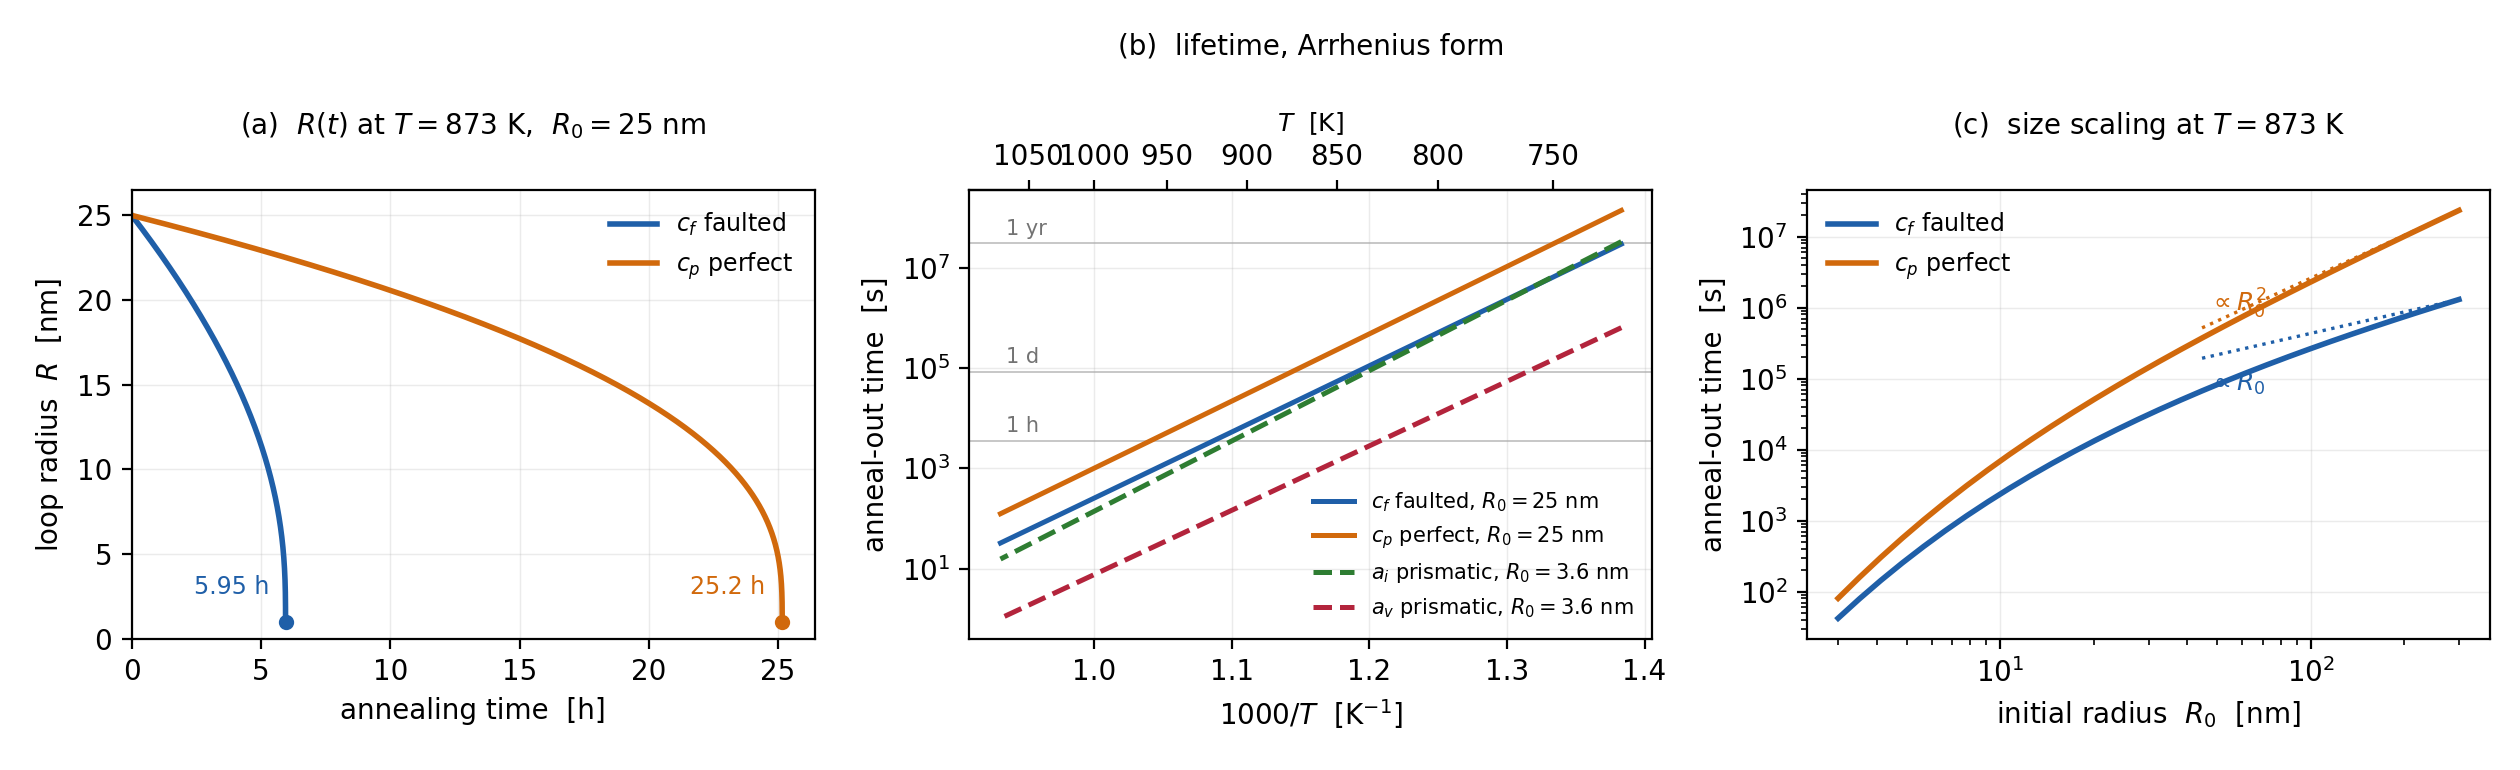
\includegraphics[width=\textwidth]{annealing_isolated_loops.png}
\caption{Thermal anneal of an isolated basal vacancy loop from
\cref{eq:isolatedR}, for the faulted state $c_f$ and the perfect state $c_p$ of
\cref{tab:cstates}. (a)~$R(t)$ at $873\,$K from $R_0=25\,$nm, on a linear time
axis: the faulted loop reaches the floor in $5.95\,$h and the perfect one in
$25.2\,$h, and the two curves have different \emph{shapes} and not merely
different rates. (b)~The anneal-out time in Arrhenius form, with the two
prismatic families added at their own reference size $R_0=3.6\,$nm; the slopes
give $Q_{\mathrm{eff}}=2.56$--$2.79\,$eV against $E^f_v+E^m_v=2.80\,$eV.
(c)~The size dependence at $873\,$K, with the two asymptotes of
\cref{eq:annealasym} drawn as guides. Produced by
\textttclr{dislocluster\_code.studies.loop\_annealing figure}.}
\label{fig:anneal-isolated}
\end{figure}

Three results, and the first two are the ones worth carrying away.

\begin{enumerate}
\item \textbf{The two states obey different laws, because one of them has a
      driving force that does not vanish with size.} In the large-loop limit
      \cref{eq:dEdmstress} tends to $\gamma_k\Omega/(\bvec\!\cdot\!\nvec)_k$ for
      the faulted state and to zero for the perfect one, so
      \begin{equation}
        \dot R\to\text{const}\;\Rightarrow\;t_{\mathrm{anneal}}\propto R_0
        \quad(c_f),
        \qquad
        \dot R\propto\frac{\ln R}{R}\;\Rightarrow\;
        t_{\mathrm{anneal}}\propto\frac{R_0^{2}}{\ln R_0}
        \quad(c_p).
        \label{eq:annealasym}
      \end{equation}
      Panel~(c) measures the local exponent $\mathrm d\ln t/\mathrm d\ln R_0$ at
      $873\,$K as $2.43\to1.85\to1.50\to1.31$ for $c_f$ at
      $15\to45\to134\to400\,$nm, and $2.83\to2.35\to2.14\to2.05$ for $c_p$ at the
      same sizes: both are converging on \cref{eq:annealasym} and neither has
      arrived at $25\,$nm, which is why panel~(a) shows two concave curves rather
      than a straight line and a curve. \textbf{A fault energy is not a
      rate constant, it is a change of kinetic law}, and no fitted annealing
      lifetime can represent both states.
\item \textbf{The lifetime is Arrhenius with an activation energy slightly below
      self-diffusion.} Panel~(b) gives $Q_{\mathrm{eff}}=2.63\,$eV ($c_f$),
      $2.67$ ($c_p$), $2.79$ ($a_i$) and $2.56\,$eV ($a_v$) against
      $E^f_v+E^m_v=2.80\,$eV. The deficit is not numerical: the rate carries
      $\overline D^{v}c^{v,\mathrm{eq}}_\infty\propto\exp[-(E^f_v+E^m_v)/k_BT]$
      \emph{times} the driving factor $\exp(\mu_k/k_BT)-1$, which itself falls
      with temperature, and the size of the deficit is therefore a direct measure
      of $\mu_k=\partial E_k/\partial m$. \textbf{A measured annealing activation
      energy below the self-diffusion value is a measurement of the binding
      energy}, and the two prismatic rows bracket the basal ones from both sides
      because $\varsigma_s(v)$ puts their $\mu_k$ on opposite sides of zero.
\item \textbf{Both prismatic characters anneal, and the vacancy one goes first.}
      At $873\,$K a $3.6\,$nm prismatic vacancy loop lasts $9.4\,$min and its
      interstitial counterpart $4.3\,$h, a factor of $27$, entirely because
      $\varsigma_s(v)$ flips the sign of a $0.19\,$eV exponent. That is the
      quantitative form of the statement in \cref{sec:basal} that one expression
      serves both characters, and it is a prediction: an anneal that removes the
      vacancy \aloop{} population well before the interstitial one, at the same
      size, is this model being right about a term it does not fit.
\end{enumerate}

\paragraph{What the applied stress does to it.} At $873\,$K and $R_0=25\,$nm,
\cref{eq:isolatedR} gives $5.95\,$h at zero stress, $3.83\,$h under
$\sigma_{33}=+200\,$MPa and $9.56\,$h under $-200\,$MPa. The sign is the
corrected one of \cref{eq:Ebstress}: a tensile stress across the basal plane
opposes a vacancy platelet and accelerates its removal, and by
\cref{eq:onethreshold} a compressive stress exceeding
$\sigma^\ast_{c_f}=\Omega^{-1}\partial E_k/\partial m=842\,$MPa would reverse it
outright. The previous sign gives the opposite answer to both, and an annealing
experiment under load is the cleanest way to tell them apart.

\paragraph{Three limits of this calculation, which \cref{sec:anneal-discrete}
exists to remove.} The loop is alone, so no neighbor re-absorbs what it emits;
the ambient field is pinned at $c^{v,\mathrm{eq}}_\infty$, where a real anneal
has it determined by the balance of every source and sink in the volume; and the
population is one loop, so nothing is said about how a \emph{distribution} of
sizes anneals --- which is the observable, and which is where \cref{sec:moments}
predicts the density falls while the surviving mean size rises.

\subsection{The same anneal by the boundary-integral Green's function}
\label{sec:anneal-greens}

\Cref{eq:isolatedR} compresses the whole of the transport into one closed-form
number, $Z^{\mathrm{iso}}_k$, and assumes the loop is a circle. \Cref{sec:bim-climb}
carries a construction that assumes neither: the boundary integral solves for the
concentration at the line rather than parameterizing it, and the loop's outline is
whatever the solved nodal velocities make it. The isolated loop is the one case
in which that construction is cheap enough to run all the way to extinction ---
one loop, no neighbors, so \cref{eq:cutoff} never fires and the pair assembly is
$N_{\mathrm{side}}^2$ with $N_{\mathrm{side}}\le128$ --- and it is therefore the
natural place to ask what \cref{eq:Ziso} is worth and what the ellipse of
\cref{eq:romstate} gives up. This subsection does both. \textbf{The conclusion is
that \cref{sec:anneal-isolated} stands}, and that the two things which do move
are worth knowing: the capture efficiency by a constant $9\%$, and the loop shape
by a factor that turns out to expose an error in \cref{eq:romselfstress}.

\paragraph{The diffusion problem, written out.} One loop, alone, in an infinite
crystal held at $c^{v,\mathrm{eq}}_\infty$. The mobile vacancy field is
quasi-steady on the climb time scale, so outside the core it satisfies the
\emph{anisotropic} steady diffusion equation with the line held at its own local
equilibrium:
\begin{equation}
  \nabla\!\cdot\!\bigl(\Dten_v\nabla c^{v}\bigr)=0
  \quad\text{outside the core tube of radius }r_0,
  \qquad
  \begin{cases}
    c^{v}(\bm x)\to c^{v,\mathrm{eq}}_\infty, & |\bm x|\to\infty,\\[2pt]
    c^{v}(\bm x)=c^{v,\mathrm{eq}}_{sk}\bigl(\kappa(\bm x),\bm\sigma\bigr),
      & \bm x\text{ on the loop line},
  \end{cases}
  \label{eq:isoBVP}
\end{equation}
closed by the kinematic statement \cref{eq:vn-common}, $v_n=\varsigma_s(v)\,
\Omega\Phi^{v}/(\bvec\!\cdot\!\nvec)_k$. \textbf{\Cref{eq:isoBVP} is a Dirichlet
problem on a closed line, and no capture efficiency appears in it anywhere} ---
which is exactly why it can be used to measure one. It is solved by the
superposition \cref{eq:superposition}, with $c^v_{\mathcal C}=
c^{v,\mathrm{eq}}_\infty$ uniform and $c^v_{\mathcal D}$ the field the climbing
line itself emits. An element climbing at $v_n$ inserts material at the
volumetric rate $(\bvec\times\hat{\bm\xi})\!\cdot\!\hat{\bm\eta}$ per unit length,
so $c^v_{\mathcal D}$ is the line integral of the anisotropic point-source Green's
function
\begin{equation}
  \nabla\!\cdot\!\bigl(\Dten_m\nabla\mathcal G_m\bigr)=-\delta(\bm x),
  \qquad
  \mathcal G_m(\bm x)=\frac{1}
    {4\pi\sqrt{\det\Dten_m}\;\sqrt{\bm x\!\cdot\!\Dten_m^{-1}\bm x}},
  \label{eq:pointsource}
\end{equation}
against that source. Carrying the network's own linear shape functions along each
chord turns the integral into the closed form \cref{eq:Gkernel} with the
elementary integrals \cref{eq:I01}, and requiring \cref{eq:isoBVP}'s Dirichlet
condition on every segment in a Galerkin sense closes the system
\cref{eq:climbsystem}. The implementation follows
\code{DislocationSegment::concentrationMatrices} term for term, core
regularization \cref{eq:ABC} included, so what is solved here is the operator
\code{GalerkinClimbSolver} assembles --- evaluated on one loop instead of a
population. One simplification is genuine and worth naming: a pure anneal has no
irradiation, so only the vacancy species is carried, and the driving
supersaturation is \cref{eq:cveq} rather than the Peach--Koehler form
\cref{eq:cline}, because \cref{sec:anneal-isolated}'s capillarity is the
thermodynamics being tested and substituting a second one would confound the
comparison.

\paragraph{What is held fixed, so that only the transport differs.} All three
constructions compared below --- \cref{eq:isolatedR}, the boundary integral, and
the ellipse ROM \cref{eq:romA,eq:romB} --- are driven by the \emph{same}
$c^{v,\mathrm{eq}}_{sk}$, built from the \emph{same} $\partial E_k/\partial m$ of
\cref{sec:anneal-isolated}, generalized from a circle to a local curvature:
\begin{equation}
  \frac{\partial E_k}{\partial m}(\kappa)
   =\frac{\gamma_k\Omega}{(\bvec\!\cdot\!\nvec)_k}
    +\frac{\langle K\rangle_k b_k^2\lambda_k^2}{4}\,\kappa\,
     \ln\frac{\mathrm e\,\alpha}{\kappa\,b_k},
  \qquad
  \kappa\to\frac1R\;\Longrightarrow\;\text{\cref{eq:dEdmstress} exactly,}
  \label{eq:dEdmlocal}
\end{equation}
since $1+\ln x=\ln(\mathrm e x)$; the reduction is checked to machine zero. So
every difference reported below is a difference of \textbf{transport} and of
nothing else. This is deliberate rather than convenient: \cref{eq:romselfstress}
uses $\mu/(1-\nu)$ where \cref{sec:anneal-isolated} uses $\langle K\rangle_k$ and
has no place for the fault term at all, and letting the ROM carry its own
thermodynamics would put a capillarity difference inside a transport comparison.

\paragraph{The kernel test, which has to come first.} In an \emph{isotropic}
medium the boundary-integral solve of a circular loop must return \cref{eq:Ziso}
itself, because the self-field of a ring of uniform strength is
$Q\ln(8R/r_0)/2\pi R$ --- the toroidal capacitance. Measured at
$N_{\mathrm{side}}=128$, with $\Dten$ replaced by $\overline D^{v}\bm I$:
\begin{center}\small
\begin{tabular}{@{}llrrr@{}}
\toprule
family & $R$ & $Z$ solved & $2\pi/\ln(8R/|\bvec_k|)$ & error\\
\midrule
$c_p$ & $5\,$nm  & $1.44469$  & $1.44359$  & $0.076\%$\\
$c_p$ & $25\,$nm & $1.05416$  & $1.05389$  & $0.026\%$\\
$a_i$ & $5\,$nm  & $1.30443$  & $1.30384$  & $0.045\%$\\
$a_i$ & $25\,$nm & $0.977648$ & $0.977407$ & $0.025\%$\\
\bottomrule
\end{tabular}
\end{center}
\textbf{This is what establishes that the boundary integral is the same physics as
$Z^{\mathrm{iso}}$ and not a different model}, and it is the reason everything
below can be attributed to the real diffusion tensor and to shape freedom rather
than to an implementation difference. It is also a non-trivial check on
\cref{eq:Gkernel}: the closed-form $I_0,I_1$ of \cref{eq:I01}, the shape-function
weighting and the core term of \cref{eq:ABC} all have to be right together for a
$0.08\%$ agreement with a result they were not built from.

\paragraph{$Z^{\mathrm{iso}}_k$ becomes an output, and is refitted.} With the
kernel verified, the capture efficiency can be \emph{read off} instead of
assumed: solve the boundary integral on a circle of radius $R$ with a unit
driving supersaturation, take the (uniform) velocity, and invert
\cref{eq:vn-common} as \cref{eq:isolatedR} writes it,
\begin{equation}
  Z^{\mathrm{iso}}_k
   =\frac{v\,(\bvec\!\cdot\!\nvec)_k}{\overline D^{v}\,\Delta c},
  \qquad
  \overline D^{v}=\bigl(\det\Dten_v\bigr)^{1/3},
  \label{eq:Zread}
\end{equation}
so that the $Z$ returned absorbs both the geometry and the tensor's departure
from the invariant $\overline D^{v}$ that \cref{eq:isolatedR} carries. Fitted over
$R=2$--$60\,$nm at $873\,$K, where $D_a=4.967\times10^{-14}$,
$D_c=9.493\times10^{-14}\,$m$^2$/s and $p_v=1.11402$ by \cref{eq:pm}:

\begin{table}[htbp]
\centering
\caption{$Z^{\mathrm{iso}}_k$ solved from \cref{eq:isoBVP} against the closed form
\cref{eq:Ziso}, at $873\,$K over $R=2$--$60\,$nm. Two one-parameter refits are
offered: $\alpha$ shifts the logarithm's argument, $f$ scales the whole
efficiency. The last column is the discrepancy as \cref{eq:Ziso} stands.}
\label{tab:Ziso-refit}
\begin{tabular}{@{}l r r r r r@{}}
\toprule
family & $\alpha$ in $2\pi/\ln(\alpha R/r_0)$ & $f$ in $f\cdot$\cref{eq:Ziso}
 & err($\alpha$) & err($f$) & err as published\\
\midrule
$c_f$ & $4.911$ & $\mathbf{1.09434}$ & $5.07\%$ & $\mathbf{0.66\%}$ & $9.07\%$\\
$c_p$ & $5.159$ & $\mathbf{1.09245}$ & $5.69\%$ & $\mathbf{0.72\%}$ & $8.98\%$\\
$a_v$ & $9.520$ & $\mathbf{0.97004}$ & $1.53\%$ & $\mathbf{0.22\%}$ & $3.18\%$\\
$a_i$ & $9.520$ & $\mathbf{0.97004}$ & $1.53\%$ & $\mathbf{0.22\%}$ & $3.18\%$\\
\bottomrule
\end{tabular}
\end{table}

Four things follow, and the second is the physical one.
\begin{enumerate}
\item \textbf{A constant factor fits; a shifted logarithm does not.} Scaling the
      efficiency leaves $\le0.7\%$ over a factor of $30$ in $R$, while shifting
      the logarithm's argument leaves $5\%$. The discrepancy is very nearly
      $R$-independent, which a multiplicative factor represents and a shift
      cannot. So the correction to \cref{eq:Ziso} is a prefactor and not a core
      radius.
\item \textbf{The sign is opposite for the two habit planes, and that is the
      diffusion tensor speaking.} Basal loops capture $9\%$ \emph{more} than
      \cref{eq:Ziso} says and prismatic loops $3\%$ \emph{less}. For vacancies
      $D_c>D_a$, so a basal loop --- whose plane lies across the fast axis --- is
      better fed than the orientation average, and a prismatic loop, whose plane
      contains it, is worse fed. $\overline D^{v}=(\det\Dten_v)^{1/3}$ is an
      invariant and cannot know which. \textbf{This is the same $p_m$ of
      \cref{eq:pm} appearing in a third place}, after the diffusion tensor and
      the Woo efficiencies of \cref{eq:Zsk}, and its appearance here is not
      fitted.
\item \textbf{$a_v$ and $a_i$ return identical $Z$}, to every digit, as they must:
      \cref{eq:Zread} is pure transport and the two families differ only in
      $\varsigma_s(v)$ and in their thermodynamics. That is a free consistency
      check on the whole construction.
\item $f$ is temperature-dependent because $D_c/D_a$ is. It is not a material
      constant, and quoting it without a temperature would be wrong.
\end{enumerate}

\paragraph{What that does to \cref{fig:anneal-isolated} and
\cref{tab:anneal-lifetime}.} Substituting the solved $Z$ into \cref{eq:isolatedR}
and integrating as before gives \cref{fig:anneal-greens}(a) and the lifetimes

\begin{center}\small
\begin{tabular}{@{}r rrr rrr@{}}
\toprule
& \multicolumn{3}{c}{$c_f$ faulted} & \multicolumn{3}{c}{$c_p$ perfect}\\
\cmidrule(lr){2-4}\cmidrule(lr){5-7}
$T$ [K] & \cref{eq:Ziso} & Green's fn.\ & ratio
        & \cref{eq:Ziso} & Green's fn.\ & ratio\\
\midrule
$773$  & $22.9\,$d   & $20.6\,$d   & $0.902$ & $0.284\,$yr & $93.6\,$d   & $0.903$\\
$823$  & $49.7\,$h   & $45.1\,$h   & $0.907$ & $9.05\,$d   & $8.22\,$d   & $0.908$\\
$873$  & $5.95\,$h   & $5.43\,$h   & $0.912$ & $25.2\,$h   & $23.0\,$h   & $0.913$\\
$923$  & $53.9\,$min & $49.4\,$min & $0.917$ & $3.69\,$h   & $3.39\,$h   & $0.918$\\
$973$  & $9.90\,$min & $9.11\,$min & $0.921$ & $39.7\,$min & $36.6\,$min & $0.922$\\
$1023$ & $2.15\,$min & $1.99\,$min & $0.924$ & $8.44\,$min & $7.81\,$min & $0.925$\\
\bottomrule
\end{tabular}
\end{center}

\textbf{Every conclusion of \cref{sec:anneal-isolated} survives, because every one
of them is a ratio or a shape and the correction is very nearly a constant.} The
absolute lifetimes fall by a uniform $8$--$10\%$; what the subsection actually
asserts does not move:
\begin{center}\small
\begin{tabular}{@{}l rrr@{}}
\toprule
quantity & \cref{eq:Ziso} & Green's function & change\\
\midrule
$t_{c_p}/t_{c_f}$ at $773\,$K & $4.5309$ & $4.5377$ & $+0.15\%$\\
$t_{c_p}/t_{c_f}$ at $1023\,$K & $3.9240$ & $3.9284$ & $+0.11\%$\\
$Q_{\mathrm{eff}}$, $c_f$ & $2.6269\,$eV & $2.6200\,$eV & $-0.26\%$\\
$Q_{\mathrm{eff}}$, $c_p$ & $2.6661\,$eV & $2.6593\,$eV & $-0.25\%$\\
$Q_{\mathrm{eff}}$, $a_i$ & $2.7905\,$eV & $2.7922\,$eV & $+0.06\%$\\
$Q_{\mathrm{eff}}$, $a_v$ & $2.5541\,$eV & $2.5558\,$eV & $+0.07\%$\\
\bottomrule
\end{tabular}
\end{center}
so \cref{tab:anneal-lifetime}'s last column stands at the precision it is quoted
to, $Q_{\mathrm{eff}}$ still sits below $E^f_v+E^m_v=2.800\,$eV by the same
margin, and the $a_i$/$a_v$ bracketing is untouched. The two \emph{shapes} of
$R(t)$ and the asymptotes \cref{eq:annealasym} are unchanged, because the fault
term is what produces them. \textbf{\Cref{eq:Ziso} was never the load-bearing
approximation in \cref{sec:anneal-isolated}; the fault term is.}

\begin{figure}[htbp]
\centering
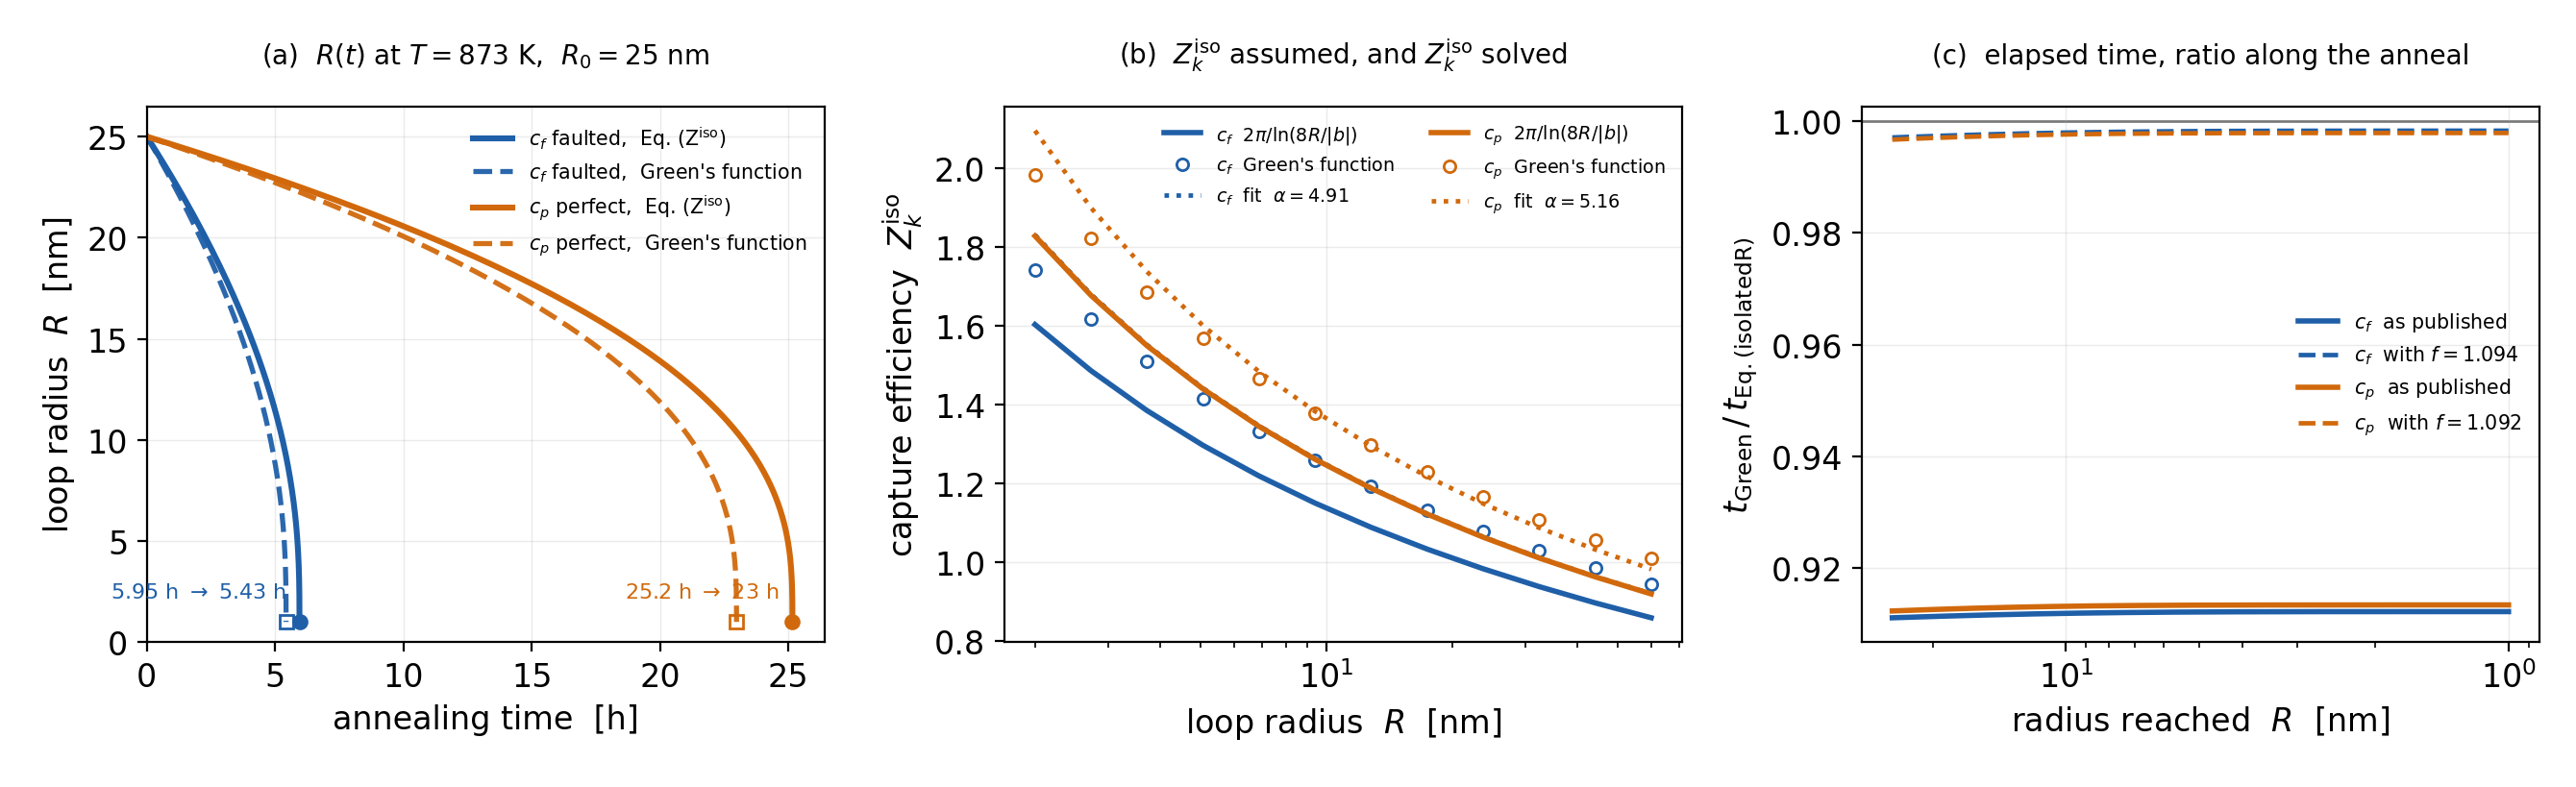
\includegraphics[width=\textwidth]{annealing_isolated_greens.png}
\caption{\Cref{fig:anneal-isolated}(a) repeated with the boundary-integral
solution superimposed. (a)~$R(t)$ at $873\,$K from $R_0=25\,$nm: solid is
\cref{eq:isolatedR} with \cref{eq:Ziso}, dashed the same law with $Z$ solved from
\cref{eq:isoBVP}. (b)~$Z^{\mathrm{iso}}_k$ assumed against
$Z^{\mathrm{iso}}_k$ solved, with the one-parameter refit of
\cref{tab:Ziso-refit}. (c)~The elapsed-time ratio along the anneal, before and
after the constant refit $f$ --- it is flat, which is the statement of item~1
above, and $f$ removes it to $0.2\%$. Produced by
\textttclr{dislocluster\_code.studies.loop\_annealing\_greens figure-rt}.}
\label{fig:anneal-greens}
\end{figure}

\paragraph{The loop shape during shrinkage.} The boundary integral carries no
shape assumption, so it answers a question \cref{eq:isolatedR} cannot pose and
\cref{eq:romA,eq:romB} can only answer inside an ellipse. Three families were
marched nodally to extinction with $N_{\mathrm{side}}=32$, alongside the ROM on
the same anneal and the same thermodynamics \cref{eq:dEdmlocal}, and the aspect
ratio $\varrho_\ell=B_\ell/A_\ell$ of \cref{eq:romstate} compared
(\cref{fig:anneal-shape}, \cref{tab:anneal-shape}).

\begin{table}[htbp]
\centering
\caption{Aspect ratio $\varrho_\ell=B_\ell/A_\ell$ down each anneal at $873\,$K,
$A_\ell\parallel[0001]$ so that $\varrho_\ell>1$ is elongation \emph{in} the basal
plane. ``Eq.'' and ``true'' are the two curvature assignments discussed below;
``geo'' and ``nrm'' the two capture-diffusivity closures of
\cref{eq:romattractor}. The basal row is the control: it must be $1$, and is.}
\label{tab:anneal-shape}
\begin{tabular}{@{}l r r rr rr@{}}
\toprule
 & & & \multicolumn{2}{c}{ROM, $\kappa$ as \cref{eq:romselfstress}}
 & \multicolumn{2}{c}{ROM, true ellipse $\kappa$}\\
\cmidrule(lr){4-5}\cmidrule(lr){6-7}
family & $R/R_0$ & Green's fn.\ & geo & nrm & geo & nrm\\
\midrule
$a_v$ & $0.83$ & $1.0102$ & $1.1259$ & $1.2252$ & $1.0393$ & $1.0793$\\
$a_v$ & $0.66$ & $1.0081$ & $1.6333$ & $1.8795$ & $1.0521$ & $1.1068$\\
$a_v$ & $0.49$ & $1.0065$ & $2.9558$ & $3.4118$ & $1.0495$ & $1.1015$\\
$a_v$ & $0.32$ & $\mathbf{1.0002}$ & $\mathbf{4.7775}$ & $4.7817$ & $\mathbf{1.0415}$ & $1.0848$\\
\addlinespace
$a_i$ & $0.83$ & $1.0472$ & $1.0703$ & $1.1403$ & $1.0654$ & $1.1310$\\
$a_i$ & $0.66$ & $1.1072$ & $1.1923$ & $1.3949$ & $1.1664$ & $1.3452$\\
$a_i$ & $0.49$ & $1.1929$ & $1.4341$ & $1.9443$ & $1.3551$ & $1.7710$\\
$a_i$ & $0.32$ & $\mathbf{1.3264}$ & $\mathbf{2.0570}$ & $3.5426$ & $\mathbf{1.8132}$ & $2.8847$\\
\addlinespace
$c_p$ & all    & $1.0000$ & $1.0000$ & $1.0000$ & $1.0000$ & $1.0000$\\
\bottomrule
\end{tabular}
\end{table}

\begin{enumerate}
\item \textbf{A basal loop cannot become an ellipse, and both constructions say
      so.} Its habit plane is the basal plane, in which $\Dten_v$ restricted to
      the plane is isotropic, so the solved velocity is uniform around the line to
      $4\times10^{-15}$ at every radius and both ROM capture diffusivities are
      identically equal. \textbf{This is the control the rest of the comparison
      rests on}, and it is also why \cref{sec:anneal-isolated}'s circular
      assumption costs nothing for the family it is applied to.
\item \textbf{\Cref{eq:romselfstress} has the two axis curvatures swapped, and
      that is the whole of the $a_v$ disagreement.} Parametrizing the habit-plane
      ellipse as $(A_\ell\cos t)\hat{\bm e}_1+(B_\ell\sin t)\hat{\bm e}_2$ gives
      $\kappa(t)=A_\ell B_\ell/(A_\ell^2\sin^2t+B_\ell^2\cos^2t)^{3/2}$, so
      \begin{equation}
        \kappa\bigl|_{A\text{ vertex}}=\frac{A_\ell}{B_\ell^{2}},
        \qquad
        \kappa\bigl|_{B\text{ vertex}}=\frac{B_\ell}{A_\ell^{2}},
        \label{eq:kappavertex}
      \end{equation}
      whereas \cref{eq:romselfstress} carries $\kappa_A=B_\ell/A_\ell^2$ and
      $\kappa_B=A_\ell/B_\ell^2$ --- the pair interchanged, verified numerically
      against the polygon circumradius on a $1{:}3$ ellipse ($0.111111$ and
      $3.00000$ against $A/B^2$ and $B/A^2$). The swap is not cosmetic: it puts
      the large curvature on the \emph{minor} axis and thereby \emph{reverses} the
      sign of the capillary shape feedback. Its own prose is the geometric
      assignment --- ``as the loop elongates, $\kappa$ rises at the major-axis
      ends, the back stress there raises $c^m_{\mathrm{eq}}$ and growth
      throttles'' --- and with that assignment restored the ROM behaves as
      described, settling at $\varrho_\ell=1.04$ against the boundary integral's
      $1.00$; as written it runs away to $4.78$, a sliver. \textbf{This is a
      correction to \cref{eq:romselfstress}, not a difference between the two
      constructions.}
\item \textbf{The two characters behave oppositely, and the exponential is why.}
      The driving supersaturation is $c^{v,\mathrm{eq}}_\infty(e^{\mu_k/k_BT}-1)$
      for a vacancy family and $c^{v,\mathrm{eq}}_\infty(1-e^{-\mu_k/k_BT})$ for
      an interstitial one, so at $\mu_k/k_BT\simeq2.5$ the logarithmic sensitivity
      $\mathrm d\ln(\text{drive})/\mathrm d\mu_k$ is $1.09/k_BT$ against
      $0.087/k_BT$. The vacancy loop's capillary shape control is
      \textbf{$12.5\times$ stiffer relative to its own drive}, which is why it
      holds $\varrho_\ell=1.00$ while $a_i$ reaches $1.33$. It is the same
      exponent that makes $a_v$ anneal $27\times$ faster in
      \cref{sec:anneal-isolated}, read on the shape instead of on the rate.
\item \textbf{Even corrected, the ROM over-reads the ellipticity} --- by
      $1.37\times$ on $a_i$ at $R/R_0=0.32$, $1.81$ against $1.33$. That residual
      is not a parameter that could be tuned away, and the next paragraph
      measures where it comes from.
\end{enumerate}

\begin{figure}[htbp]
\centering
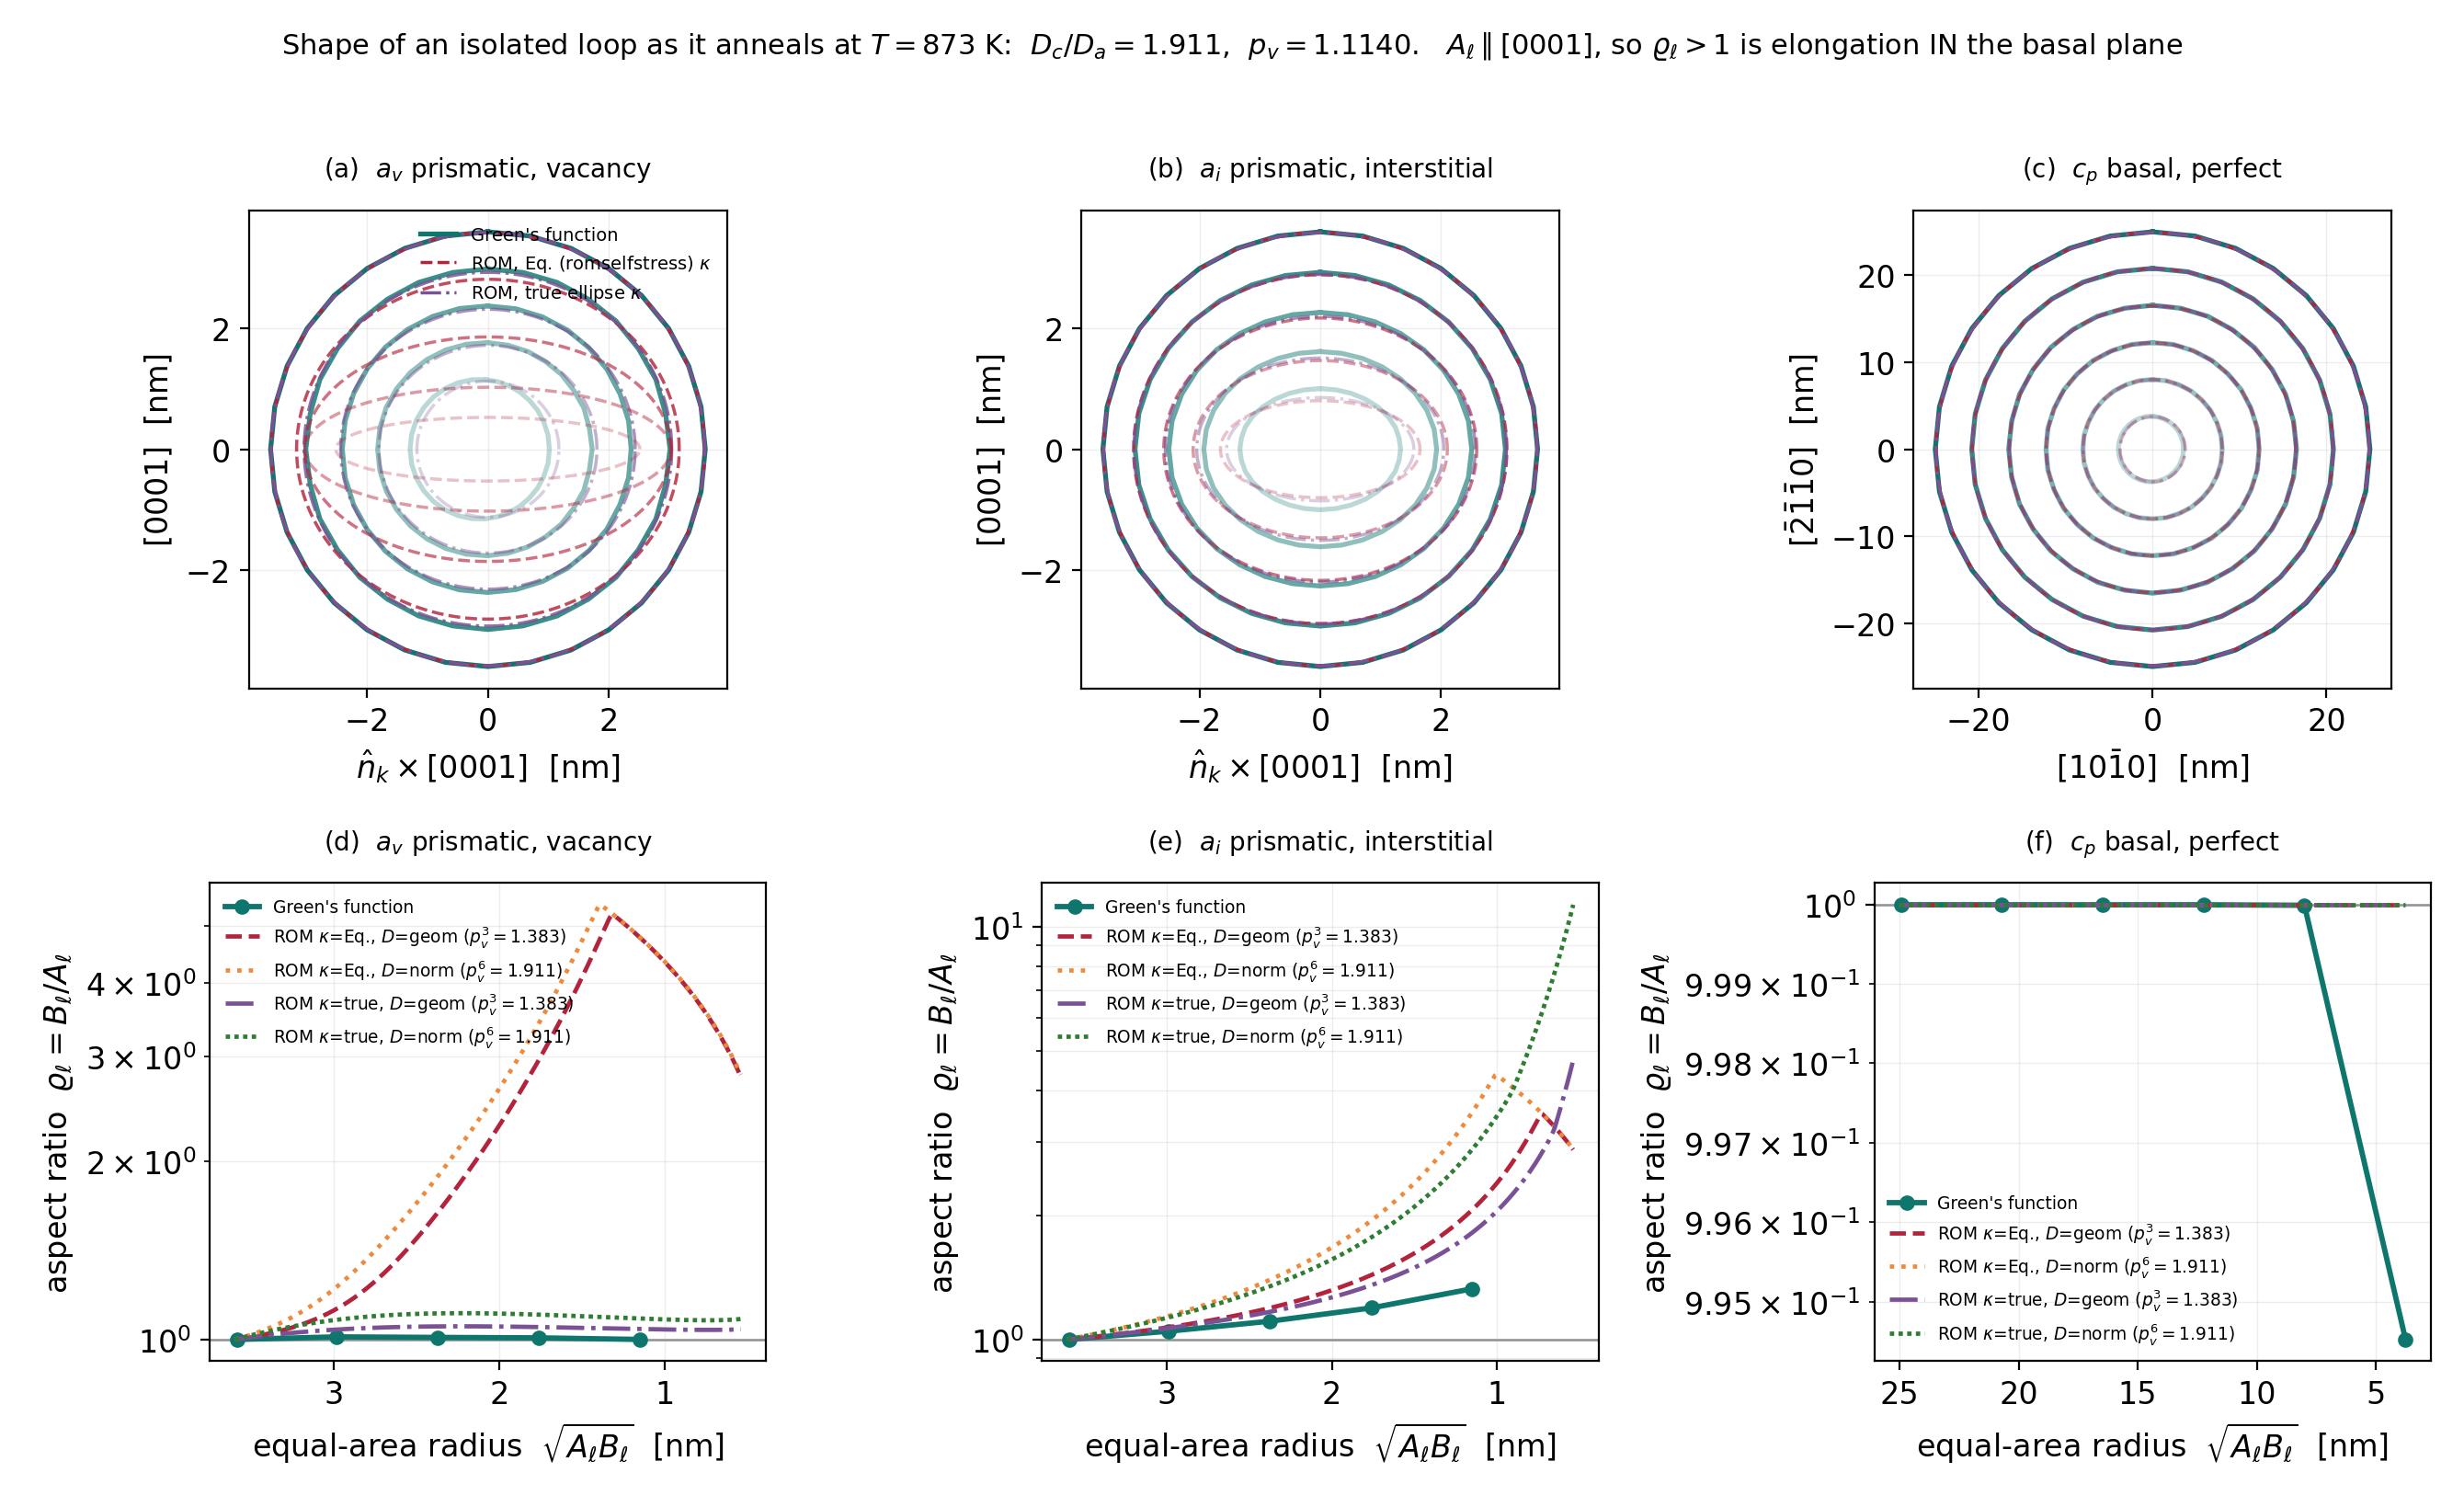
\includegraphics[width=\textwidth]{annealing_loop_shape.png}
\caption{Loop shape during shrinkage at $873\,$K, where $D_c/D_a=1.911$ and
$p_v=1.1140$. Top row, the outlines at six equal-area radii: solid is the nodal
boundary-integral solve, dashed the ROM with \cref{eq:romselfstress}'s curvature
assignment, dash-dotted the ROM with \cref{eq:kappavertex}. Bottom row, the
aspect ratio on a logarithmic axis, with both capture-diffusivity closures of
\cref{eq:romattractor}. (a,d)~$a_v$, where the uncorrected ROM collapses to a
sliver and the solve stays circular; (b,e)~$a_i$, the one family whose shape
genuinely moves; (c,f)~$c_p$ basal, the control, circular in every column.
Produced by \textttclr{...loop\_annealing\_greens figure-shape}.}
\label{fig:anneal-shape}
\end{figure}

\paragraph{Why the two shapes differ, and by how much.} Item~4 above is a
statement that needs an account rather than an assertion, because the gap is
large --- $1.81$ against $1.33$ on $a_i$ --- and because the obvious explanation
is the wrong one. The kinematics have to come first. Writing
$A_\ell=R/\sqrt{\varrho}$ and $B_\ell=R\sqrt{\varrho}$ at fixed area, with both
axes retreating,
\begin{equation}
  \frac{\mathrm d\ln\varrho_\ell}{\mathrm dt}
   =\frac{|v_A|}{A_\ell}-\frac{|v_B|}{B_\ell}
   =\frac{|v_B|}{R}\,\varrho_\ell^{-1/2}\,
    \underbrace{\left[\varrho_\ell\frac{v_A}{v_B}-1\right]}_{\textstyle
      E(\varrho_\ell)},
  \label{eq:elongdrive}
\end{equation}
so it is $E$, not $v_A/v_B$, that drives elongation, and a steady shape needs
$E=0$. \textbf{In the ROM $v_A/v_B=D^{(A)}_m/D^{(B)}_m=p_m^{3}$ is a constant},
fixed by crystallography and independent of the shape, so
$E_{\mathrm{ROM}}=p_m^{3}\varrho_\ell-1$ grows without bound. In the boundary
integral $v_A/v_B$ is solved, and it does not stay constant.

\begin{table}[htbp]
\centering
\caption{Axis velocities on a \emph{fixed} ellipse of equal-area radius
$3.6\,$nm at $873\,$K under a \emph{uniform} drive, so that capillarity plays no
part and only transport and geometry act. The isotropic column replaces
$\Dten_v$ by $\overline D^{v}\bm I$, where the ROM predicts $v_A/v_B=1$ at every
aspect ratio: whatever the solve gives instead is the term the ROM does not have.
$E$ is the elongation drive of \cref{eq:elongdrive}.}
\label{tab:shape-mechanism}
\begin{tabular}{@{}r rr rrr@{}}
\toprule
 & \multicolumn{2}{c}{$v_A/v_B$ solved} & \multicolumn{3}{c}{elongation drive}\\
\cmidrule(lr){2-3}\cmidrule(lr){4-6}
$\varrho_\ell$ & isotropic $\Dten$ & true $\Dten$
 & $E$ solved & $E_{\mathrm{ROM}}$ & ratio\\
\midrule
$1.00$ & $\mathbf{1.0000}$ & $1.2967$ & $0.2967$ & $0.3825$ & $0.776$\\
$1.15$ & $0.9743$ & $1.2552$ & $0.4434$ & $0.5899$ & $0.752$\\
$1.35$ & $0.9439$ & $1.2013$ & $0.6217$ & $0.8664$ & $0.718$\\
$1.60$ & $0.9086$ & $1.1343$ & $0.8149$ & $1.2121$ & $0.672$\\
$2.00$ & $0.8541$ & $1.0237$ & $1.0475$ & $1.7651$ & $0.594$\\
$2.50$ & $0.7860$ & $0.8685$ & $\mathbf{1.1712}$ & $2.4563$ & $0.477$\\
$3.00$ & $0.7147$ & $0.6689$ & $1.0068$ & $3.1476$ & $\mathbf{0.320}$\\
\bottomrule
\end{tabular}
\end{table}

\begin{enumerate}
\item \textbf{The dominant term is a shape-dependent capture efficiency, and the
      ROM has none.} \Cref{eq:isoBVP} imposes a \emph{Dirichlet} condition on the
      line, so it is a capacitance problem, and the source density it induces
      concentrates where the curvature is high --- the same point effect that
      puts charge on the sharp end of a conductor. As a loop elongates, the sharp
      end of its long axis therefore emits faster and retreats faster, and the
      elongation limits itself. The isotropic column of
      \cref{tab:shape-mechanism} is that effect alone: it is
      $\mathbf{1.0000}$ at $\varrho_\ell=1$, exactly, by symmetry --- which is
      simultaneously a check on the solver and the reason this term does
      \emph{not} contaminate the closure exponent measured on a circle --- and it
      falls as $\varrho_\ell^{-0.316}$ thereafter. \textbf{Nothing in
      \cref{eq:romA,eq:romB} can reproduce it}, because their two endpoints are
      coupled to each other only through the shared $L_{\mathrm{cap}}$ and never
      through a field.
\item \textbf{The consequence is that the two elongation drives diverge rather
      than differing by a constant.} $E_{\mathrm{ROM}}$ is linear in
      $\varrho_\ell$ for ever; the solved $E$ rises, peaks at $1.17$ near
      $\varrho_\ell=2.5$ and \emph{turns over}. Their ratio falls from $0.78$ at
      $\varrho_\ell=1$ to $0.32$ at $\varrho_\ell=3$. \textbf{So the disagreement
      is not an offset but a compounding one, growing with how far the loop has
      already elongated} --- which is exactly the pattern of
      \cref{tab:anneal-shape}, where $a_v$ agrees to $3\%$ at $R/R_0=0.83$ and
      $a_i$ disagrees by $37\%$ at $R/R_0=0.32$.
\item \textbf{Capillarity is \emph{not} the explanation, and this is worth
      establishing rather than assuming.} The natural suspicion is that the ROM
      resolves the capillary back stress at two vertices where the solve resolves
      it at every node. Re-running the nodal anneal with the driving
      supersaturation frozen at the equal-area curvature --- which keeps its
      magnitude and removes its shape feedback entirely --- gives
      \begin{center}\small
      \begin{tabular}{@{}r rrr@{}}
      \toprule
      $R/R_0$ & $\varrho_\ell$ nodal $\kappa$ & $\varrho_\ell$ frozen $\kappa$ & ratio\\
      \midrule
      $0.82$ & $1.0491$ & $1.0534$ & $1.004$\\
      $0.65$ & $1.1113$ & $1.1332$ & $1.020$\\
      $0.47$ & $1.2022$ & $1.2575$ & $1.046$\\
      $0.30$ & $1.3468$ & $1.4613$ & $\mathbf{1.085}$\\
      \bottomrule
      \end{tabular}
      \end{center}
      so the capillary shape feedback is worth $8.5\%$ in $\varrho_\ell$ at the
      end of the anneal --- \textbf{when the whole of the ROM's excess is
      $37\%$}. Removing it \emph{entirely} could account for at most a quarter of
      the gap, and the ROM does not remove it entirely; it carries it at two
      points. Capillary resolution is therefore a real but third-order
      contribution, and the geometric term of item~1 is the explanation.
\item \textbf{A residual $6\%$ is present even at $\varrho_\ell=1$}, where the
      solved $v_A/v_B=1.2967$ against the ROM's $p_v^3=1.3825$. That is the
      closure exponent of the next paragraph, $q=2.41$ rather than $3$, and it is
      a statement about \emph{transport} on a circle rather than about shape. It
      sets the initial rate at which the two constructions part company; items~1
      and~2 are what make the parting grow.
\end{enumerate}

\textbf{Read together, the four items say something about when the ROM may be
used.} Its two ODEs are local --- each endpoint sees its own diffusivity and its
own curvature, and nothing else --- whereas \cref{eq:climbsystem} makes every
point of the line see every other. That difference is invisible on a circle,
where the ROM's error is the $6\%$ of item~4, and it grows as the square of
nothing in particular but monotonically with departure from a circle. \textbf{The
ROM is therefore reliable for the \aloop{} population it was built for},
\cref{tab:climb-selection}, whose loops sit at $\Theta_k=0.081$ and stay close to
circular through a march, and it should not be trusted for a shape prediction
once $\varrho_\ell$ exceeds about $1.5$ --- which, by \cref{eq:romapproach}, is
also where its own approach-to-attractor argument stops being the limiting
consideration.

\paragraph{Which capture-diffusivity closure, settled.} \Cref{sec:ellipse-rom}
leaves \cref{eq:romattractor} open --- ``\emph{this is not settled} \dots only a
nodal solve of the same case can collapse it'' --- because the diffusivity feeding
the end of the $[0001]$ axis is not fixed by geometry: the geometric mean gives an
axis-velocity ratio $D^{(A)}_m/D^{(B)}_m=p_m^{3}$ and the normal projection
$p_m^{6}$. \textbf{The isolated loop is a nodal solve of exactly that case.} Put a
\emph{circular} prismatic loop in the boundary-integral solver with a
\emph{uniform} drive, so that the only thing which can make the two axis endpoints
move at different speeds is the diffusion tensor, and read the ratio off as an
effective exponent $q=\ln(v_A/v_B)/\ln p_v$:
\begin{center}\small
\begin{tabular}{@{}r r rrrr@{}}
\toprule
$T$ [K] & $p_v$ & $q$ at $R=2\,$nm & $3.6\,$nm & $10\,$nm & $25\,$nm\\
\midrule
$773$  & $1.12969$ & $2.095$ & $2.398$ & $2.625$ & $2.720$\\
$873$  & $1.11402$ & $2.116$ & $2.408$ & $2.630$ & $2.724$\\
$1023$ & $1.09652$ & $2.137$ & $2.419$ & $2.635$ & $2.727$\\
\bottomrule
\end{tabular}
\end{center}
against $q=3$ (geometric mean) and $q=6$ (normal projection). \textbf{$q$ is
independent of temperature --- hence of $p_v$ --- to three decimal places, and
rises with $R$ toward $3$.} The geometric mean is the large-loop limit and the
normal projection is not a candidate at all; the shortfall at small $R$ is the
core regularization blunting the anisotropy, and it is a \emph{size} effect rather
than a material one, so it is a correction to the closure and not a competitor to
it. \textbf{This removes the factor of $p_m^{3}$ that \cref{sec:ellipse-rom}
requires to be quoted with any ROM ellipticity.}

\paragraph{One further correction the comparison forces.} \Cref{eq:romA} writes
the arrival rate as $Z_{sk,m}D^{(A)}_m/L_{\mathrm{cap}}$, whereas
\cref{eq:isolatedR} and the boundary integral both write it as
$Z^{\mathrm{iso}}_k\overline D^{v}/\Omega$ --- a concentration is an atom fraction,
so $c/\Omega$ is a number density and no length appears. Matching the two at the
reference radius gives
\begin{equation}
  L_{\mathrm{cap}}
   =\frac{\Omega\,Z_{sk,v}}{b^{2}\,Z^{\mathrm{iso}}_k(R)}
   \;\simeq\;\frac{\Omega}{b^{2}}=0.690\,|\bvec|=0.223\,\mathrm{nm},
  \label{eq:Lcap-calib}
\end{equation}
that is $0.16$--$0.23\,$nm across the four families, against the screening length
\cref{eq:screening} of $\simeq59\,$nm that \cref{sec:ellipse-rom} defaults it to.
\textbf{At that default the ROM's isolated-loop climb rate is $260$--$370\times$
too slow.} \Cref{sec:ellipse-rom} is right that $L_{\mathrm{cap}}$ enters both
axis equations identically and therefore sets the time scale alone and cancels
from the aspect ratio --- so \cref{tab:anneal-shape} is untouched by this, and
\cref{eq:Lcap-calib} is a calibration rather than a repair --- but it means no ROM
\emph{lifetime} may be quoted at the screening-length default.

\paragraph{Three limits of this comparison.} The loop is isolated, so nothing here
tests the pair assembly \cref{eq:Kclimb} or the truncation \cref{eq:cutoff}, which
are what make the boundary integral expensive on a population and are measured in
\cref{sec:climb-selection} instead. Only the vacancy species is carried, which is
exact for a pure anneal and not for a march. And the core convention is
$r_0=|\bvec_k|$ throughout, to match \cref{eq:Ziso}'s own $\ln(8R/|\bvec|)$,
where the tutorials set $\code{coreSize}=2\,b$; changing it moves $Z$ by roughly
$\ln2/\ln(8R/b)$, which is $11\%$ at $25\,$nm and is a convention difference
rather than a physical one. Below $\simeq3\,$nm the polygon segments approach the
core radius and the last snapshot of each shape march is discretization-limited;
the $c_p$ control measures the size of that as $\varrho_\ell=0.9945$ instead of
$1$ at the smallest radius drawn.

\subsection{Annealing of loop populations}
\label{sec:anneal-population}

\Cref{sec:anneal-isolated} closed by naming three limits of the isolated-loop
calculation, and the first two are the same limit twice: the loop has no
neighbors, so nothing re-absorbs what it emits, and the ambient field is
\emph{imposed} at $c^{v,\mathrm{eq}}_\infty$ rather than solved for. A real
post-irradiation anneal has neither. When the source is switched off, thermal
vacancies are emitted by some components of the microstructure and absorbed by
others, and the concentration every loop actually sees is whatever that exchange
settles at. This subsection solves for it, and the result changes not only the
rates of \cref{fig:anneal-isolated} but the \emph{separation} between the two
families and, once a size distribution is admitted, the qualitative character of
the anneal itself.

\paragraph{The balance, and why it closes on vacancies alone.} A long time after
the source is off, thermal emission of interstitials is negligible --- $E^f_i=3.0$
against $E^f_v=1.6\,$eV, so $c^{i,\mathrm{eq}}_\infty/c^{v,\mathrm{eq}}_\infty
=e^{-1.4/k_BT}=1.0\times10^{-8}$ at $873\,$K --- and with it mutual
recombination. What remains is a pure vacancy balance
\citep{ghoniem_thesis}:
\begin{equation}
  \Bigl[\text{total rate of thermal vacancy emission}\Bigr]
  =\Bigl[\text{total rate of vacancy removal}\Bigr].
  \label{eq:vbalance}
\end{equation}
Component $k$ of the microstructure exchanges vacancies with the matrix at the
rate its own sink strength sets: it emits $S_k\overline D^{v}
c^{v,\mathrm{eq}}_{k}/\Omega$ and absorbs $S_k\overline D^{v}\bar c_v/\Omega$
per unit volume, so \cref{eq:vbalance} reads $\sum_k S_k c^{v,\mathrm{eq}}_{k}
=\bar c_v\sum_k S_k$ and
\begin{equation}
  \boxed{\;
  \bar c_v=\frac{\displaystyle\sum_{k} S_k\,c^{v,\mathrm{eq}}_{k}}
                {\displaystyle\sum_{k} S_k}\;},
  \qquad
  S_k=Z_{k,v}\,\rho^k_{sL},
  \qquad
  S_N=Z_{N,v}\,\rho_N .
  \label{eq:cbar}
\end{equation}
Two things about \cref{eq:cbar} are worth stating before anything is computed
from it. First, $\overline D^{v}$ and $\Omega$ cancel: \textbf{$\bar c_v$ is a
property of the microstructure and the temperature alone}, and carries no
mobility, which is why it can be evaluated on a state without integrating
anything. Second, \cref{eq:cbar} is not an imported construction ---
\textbf{its denominator has exactly the form of $k^2_v$ in \cref{eq:KL_matrix}},
the same sum of $Z\rho^k_{sL}$ over $\mathcal F_L$ plus the same $Z_{N,v}\rho_N$,
and is that quantity identically when $Z_{k,v}$ is taken to be the mean-field
$Z_{sk,v}$ of \cref{eq:Zsk}. The remote concentration is the
sink-strength-weighted average of the levels the components would each impose on
their own, and the model already assembles those weights for the mobile block.
Nothing new is fitted here. Which $Z$ is used, and the one thing that must not be
done with the choice, is taken up at the end of this subsection.

\paragraph{Each family's own level, and the ladder they form.} Every component
enters \cref{eq:cbar} through the concentration it is individually in equilibrium
with, which is \cref{eq:cveq} unchanged:
\begin{equation}
  c^{v,\mathrm{eq}}_{k}(R)
  =c^{v,\mathrm{eq}}_\infty
   \exp\!\left\{\frac{\varsigma_s(v)\,\mu_k(R)+\Sigma_k\Omega}{k_BT}\right\},
  \qquad
  \mu_k=\frac{\partial E_k}{\partial m}
       =\frac{\gamma_k\Omega}{(\bvec\!\cdot\!\nvec)_k}
        +\frac{\langle K\rangle_k b_k^2\lambda_k^2}{4R}
         \Bigl[1+\ln\frac{\alpha R}{b_k}\Bigr].
  \label{eq:levels}
\end{equation}
So the nine families of \cref{eq:families} arrange themselves on a ladder, and
$\varsigma_s(v)$ decides which rung each takes: the basal vacancy chain
$(v,c_f),(v,c_p)$ and the prismatic vacancy variants $(v,a_{1,2,3})$ sit
\emph{above} $c^{v,\mathrm{eq}}_\infty$, the prismatic interstitial variants
$(i,a_{1,2,3})$ sit \emph{below} it, and the network dislocations sit
\emph{on} it, having neither fault nor curvature. This is
\citeauthor{ghoniem_thesis}'s Fig.~(9.16) with voids removed --- $\alpha$-Zr has
none in this model --- and the loop families of \cref{eq:families} in their place.

The growth law needs no modification at all: \cref{eq:isolatedR} with $\bar c_v$
substituted for $c^{v,\mathrm{eq}}_\infty$,
\begin{equation}
  \frac{\mathrm dR_k}{\mathrm dt}
   =\varsigma_s(v)\,\frac{Z_{k,v}\,\overline D^{v}}
                         {(\bvec\!\cdot\!\nvec)_k}
    \left[\bar c_v-c^{v,\mathrm{eq}}_{k}(R_k)\right],
  \label{eq:popR}
\end{equation}
is the whole of the change. Because $\bar c_v$ is a weighted average it always
lies between the extreme rungs, so \textbf{in a mixed microstructure something is
always emitting while something else is absorbing}. Which of the two a given
family does follows from where its rung sits; what that does to its \emph{size}
then depends on its character, and the two questions must be kept apart:

\begin{center}\small
\begin{tabular}{@{}llll@{}}
\toprule
rung relative to $\bar c_v$ & role & vacancy family & interstitial family\\
\midrule
above & net emitter  & shrinks & grows\\
below & net absorber & grows   & shrinks\\
\bottomrule
\end{tabular}
\end{center}

\paragraph{The three prismatic variants, and what a stress does to them.} At zero
deviatoric stress the three variants are equivalent by symmetry
(\cref{sec:families}), share one rung and one fate. Under load they do not: the
resolved stress $\Sigma_k=\hat{\bm a}_k\cdot\bm\sigma\cdot\hat{\bm a}_k$ enters
\cref{eq:levels} directly, so each variant's rung shifts by
$\exp(\Sigma_k\Omega/k_BT)$ while $\bar c_v$ remains a single number. Under
$\sigma_{11}=200\,$MPa along $[10\bar10]$, $a_1$ takes the full stress and $a_2$,
$a_3$ take $\sigma\cos^2 60^\circ=\sigma/4$, and their levels separate by a
factor of $1.34$ at $873\,$K. \textbf{On the reference microstructure that moves
rates and not signs}: all three still shrink, at $2.4837$ against
$2.5012\times10^{-13}\,$m/s, a $0.7\%$ split, because $\bar c_v=1.47\,
c^{v,\mathrm{eq}}_\infty$ sits nearly two decades above every prismatic rung and
lifting one of them to it would take $2065\,$MPa. Restricted to the prismatic
family alone --- which is what \cref{eq:cbar} gives for a microstructure with no
\cloop{} population and no network --- $\bar c_v$ falls \emph{inside} the
variants' own spread by construction, at $0.0333\,c^{v,\mathrm{eq}}_\infty$
against rungs at $0.0401$ and $0.0300$, and the signs do separate:
\textbf{$a_1$ grows while $a_2$ and $a_3$ dissolve, under a purely thermal
anneal with no irradiation at all.} That is variant selection by stress with no
production term anywhere in it, and it is a prediction the resolved layout of
\cref{eq:families} makes and a lumped \aloop{} population cannot.

\paragraph{One size per family: the reference microstructure.} The
microstructure annealed below is the one the $300\,$nm hardening cube of
\cref{sec:observables-mech} carries, and it is specified by the continuum state it was
drawn from rather than by the draw: \code{cube\_population} samples the interior
per-family state of the matched self-consistent march, so the two agree to the
integer draw. At $0.1\,$dpa the cube holds $21$ \cloop{} and $3\times98$
\aloop{} loops in $2.702\times10^{-20}\,$m$^3$, that is
$N_c=7.77\times10^{20}$ and $N_a=1.088\times10^{22}\,$m$^{-3}$, against
$7.68\times10^{20}$ and $1.092\times10^{22}$ in the state itself --- $1.2\%$ and
$0.4\%$. Nothing is refused by the cube at this dose, so the anneal is run on the
state, which carries the mean radii the draw needs anyway.

\Cref{fig:anneal-ladder} draws \cref{eq:cbar} for that state at $873\,$K. At $0.1\,$dpa the \cloop{} family sits at
$4.99\,c^{v,\mathrm{eq}}_\infty$ and carries $22\%$ of the sink strength, the
three \aloop{} variants together sit at $0.027$ and carry $43\%$, and the network
carries the remaining $34\%$ at $c^{v,\mathrm{eq}}_\infty$ exactly. The result is
$\bar c_v=1.46\,c^{v,\mathrm{eq}}_\infty$: \textbf{the matrix is supersaturated in
vacancies by half again for the whole anneal}, held there by the \cloop{} loops'
own emission. Both families shrink --- the \cloop{} loops because their rung is
above the line, the \aloop{} loops because theirs is below it --- and
\cref{tab:anneal-population} is what that costs each of them.

\begin{figure}[htbp]
\centering
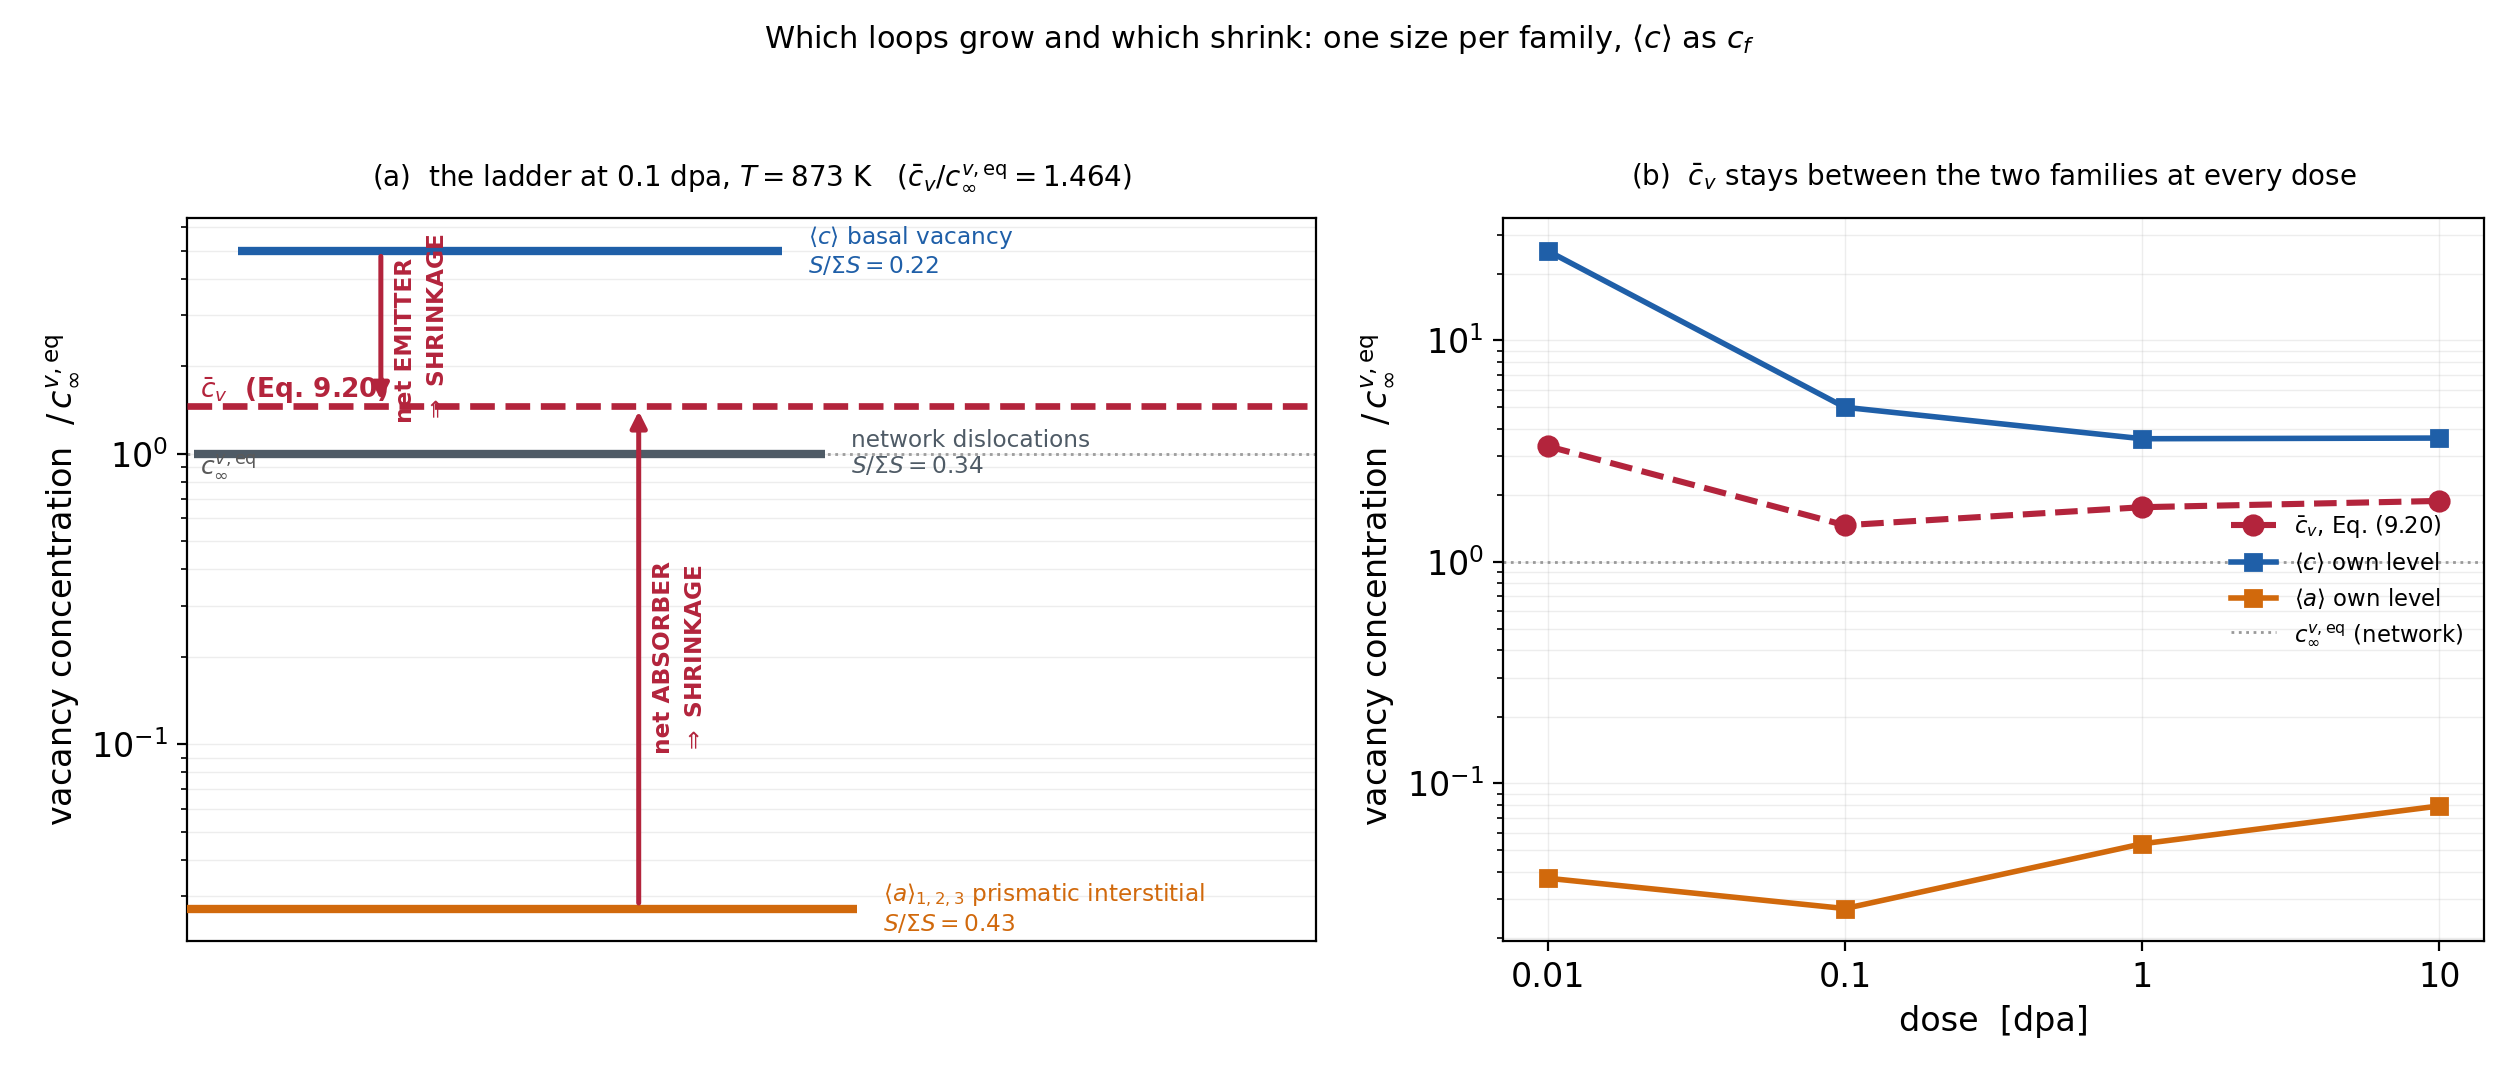
\includegraphics[width=\textwidth]{annealing_ladder.png}
\caption{The concentration ladder of \cref{eq:cbar}, one size per family, on the
interior state of the reference march at $873\,$K. (a)~Each rung is a component's
own $c^{v,\mathrm{eq}}_k$ and its width is that component's weight $S_k/\sum S_k$
in \cref{eq:cbar}; the dashed line is the solved $\bar c_v$. The \cloop{} loops
are net emitters and the \aloop{} loops net absorbers, and \emph{both} shrink,
because $\varsigma_s(v)$ has opposite signs for them. (b)~The same across dose:
$\bar c_v$ tracks between the two families at every one, never leaving the
interval the rungs bracket. Produced by
\textttclr{dislocluster\_code.studies.loop\_annealing\_population figure-ladder}.}
\label{fig:anneal-ladder}
\end{figure}

\begin{table}[htbp]
\centering
\caption{\Cref{sec:anneal-isolated}'s anneal repeated on the reference
microstructure at $873\,$K, with $\bar c_v$ solved from \cref{eq:cbar} at every
step instead of pinned at $c^{v,\mathrm{eq}}_\infty$. \cloop{} is mapped onto the
faulted state $c_f$, whose $(\bvec\!\cdot\!\nvec)=c/2$ is the geometry the march
carries. The last two columns are the same $\bar c_v$ computed with the two
capture efficiencies discussed at the end of this subsection; the calculation
itself uses $Z^{\mathrm{iso}}$ throughout, and their spread is the honest
uncertainty on the weighting.}
\label{tab:anneal-population}
\begin{tabular}{@{}r r r r r r r r r@{}}
\toprule
 & \multicolumn{2}{c}{state}
 & \multicolumn{2}{c}{\cloop{} lifetime}
 & \multicolumn{2}{c}{\aloop{} lifetime}
 & \multicolumn{2}{c}{$\bar c_v/c^{v,\mathrm{eq}}_\infty$}\\
\cmidrule(lr){2-3}\cmidrule(lr){4-5}\cmidrule(lr){6-7}\cmidrule(lr){8-9}
dpa & $R_c$ [nm] & $R_a$ [nm]
 & isolated & population & isolated & population
 & $Z_{sk,v}$ & $Z^{\mathrm{iso}}$\\
\midrule
$0.01$ & $5.43$  & $2.51$ & $6.30\,$min & $6.89\,$min & $2.29\,$h & $2.40\,$h   & $3.291$ & $3.330$\\
$0.1$  & $25.84$ & $2.19$ & $6.37\,$h   & $8.96\,$h   & $1.76\,$h & $65.8\,$min & $1.857$ & $1.464$\\
$1$    & $57.15$ & $2.96$ & $29.1\,$h   & $53.6\,$h   & $3.10\,$h & $97.2\,$min & $2.116$ & $1.766$\\
$10$   & $55.82$ & $3.64$ & $27.9\,$h   & $51.0\,$h   & $4.36\,$h & $2.14\,$h   & $2.188$ & $1.885$\\
\bottomrule
\end{tabular}
\end{table}

Three results, and the third is the one that matters for interpreting an
experiment.

\begin{enumerate}
\item \textbf{The population coupling pushes the two families in opposite
      directions.} At $1\,$dpa the \cloop{} lifetime rises by $1.84\times$ and the
      \aloop{} lifetime falls to $0.52\times$. The mechanism is the one
      \citeauthor{ghoniem_thesis} states in a sentence: the vacancy loops emit
      vacancies, which holds the \cloop{} population up against its own
      dissolution and feeds the \aloop{} loops the vacancies that destroy them.
      Neither effect exists in \cref{eq:isolatedR}, and neither is small.
\item \textbf{The separation between the two families is amplified, not merely
      shifted.} Isolated, the ratio $t_{\cloop{}}/t_{\aloop{}}$ is $3.6$ at
      $0.1\,$dpa; in the population it is $8.2$. Whatever is inferred from a
      measured pair of annealing times --- and \cref{sec:anneal-isolated}'s
      $Q_{\mathrm{eff}}$ argument is exactly such an inference --- the isolated
      calculation gets the separation wrong by more than a factor of two.
\item \textbf{The ambient is not a constant, because the microstructure that sets
      it is the one being dissolved.} \Cref{fig:anneal-reference}(b) tracks
      $\bar c_v$ through the anneal: it steps up when the \aloop{} population
      vanishes at $66\,$min, removing the only rung below the line, and then runs
      away by more than an order of magnitude as the surviving \cloop{} loops
      shrink and their own capillary level climbs. The reverse ordering at
      $0.01\,$dpa is the same effect read backwards: there the \cloop{} loops are
      only $5.4\,$nm and are gone in seven minutes, after which the \aloop{}
      loops anneal in what is very nearly isolation, and their population
      lifetime comes back to $1.05\times$ the isolated one. \textbf{An annealing
      model that fits one effective supersaturation to a whole anneal is fitting
      an average over that.}
\end{enumerate}

\begin{figure}[htbp]
\centering
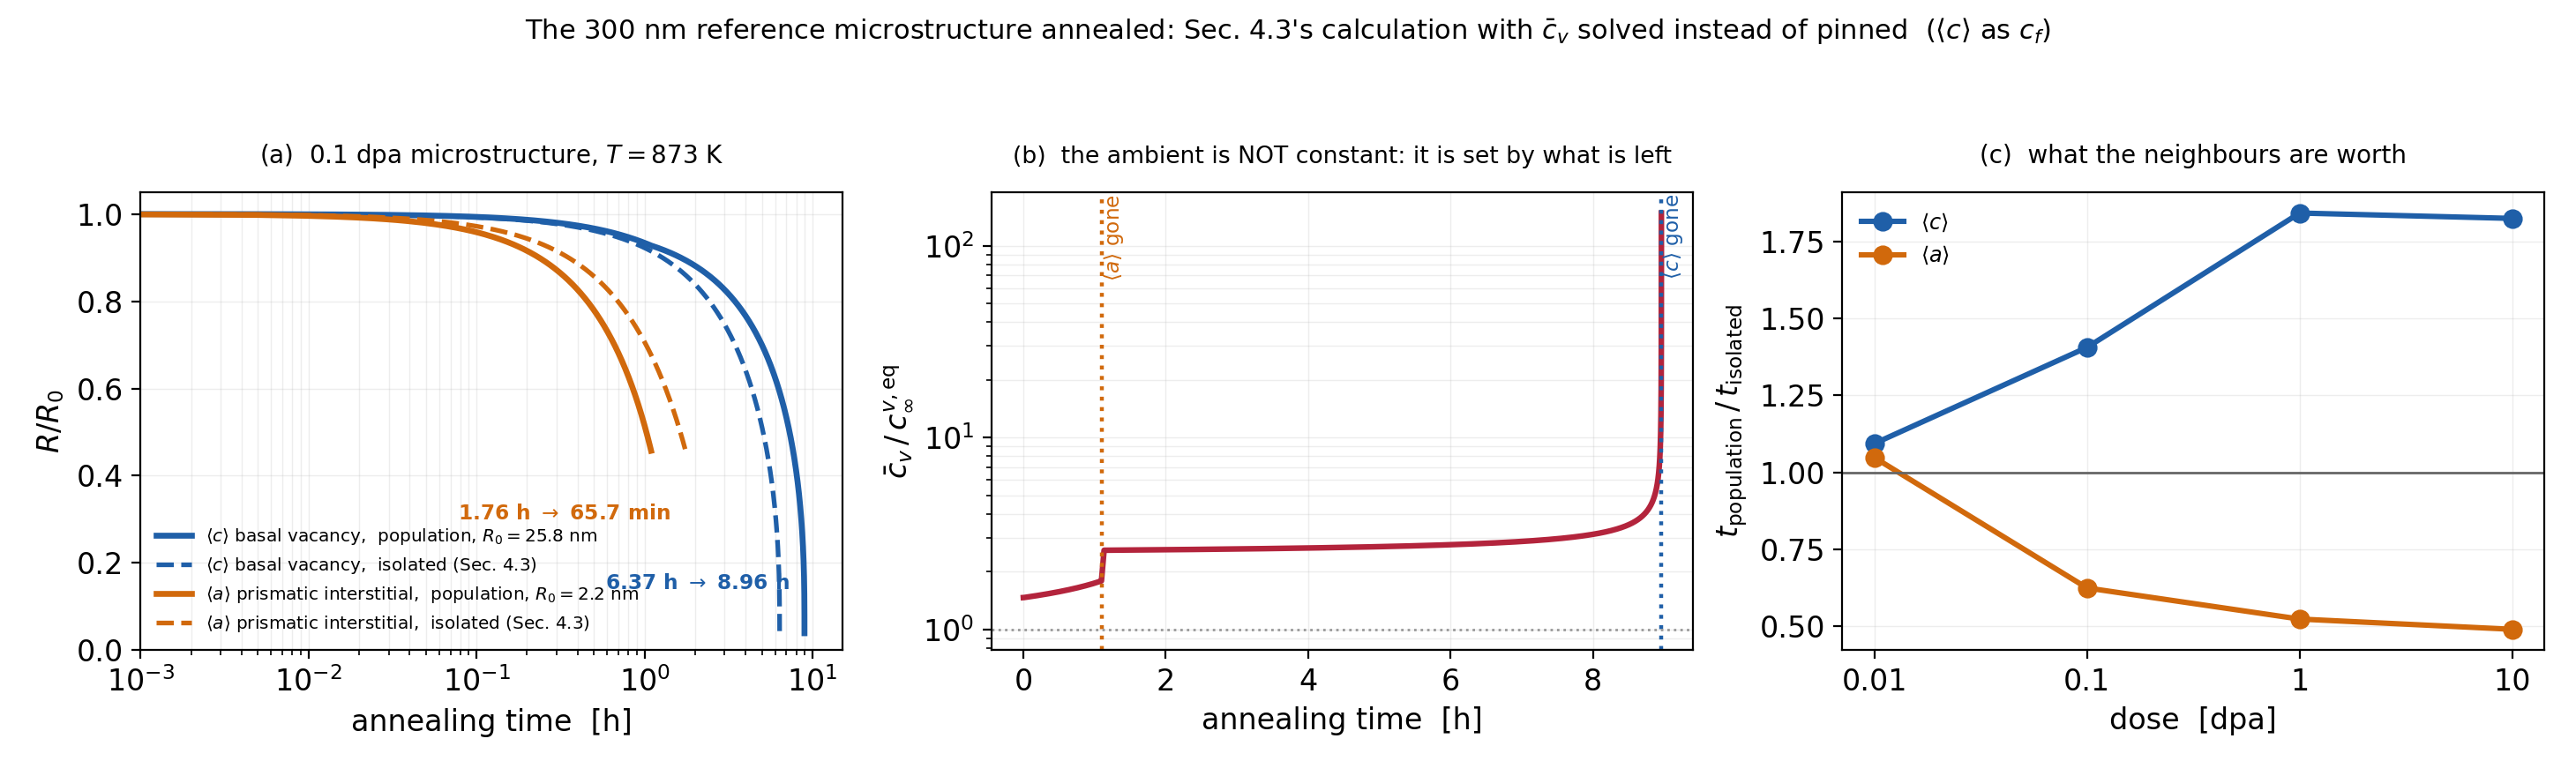
\includegraphics[width=\textwidth]{annealing_population_reference.png}
\caption{\Cref{sec:anneal-isolated}'s calculation repeated on the reference
microstructure. (a)~$R/R_0$ against annealing time on a logarithmic axis --- the
two families differ by a factor of $12$ in size and $8$ in lifetime, so no linear
axis shows both --- with the isolated trajectory of \cref{eq:isolatedR} dashed
beside each. (b)~$\bar c_v$ through the anneal, with the two extinction times
marked. (c)~The lifetime ratio across dose: the neighbors are worth a factor of
two, in opposite directions for the two families. Produced by
\textttclr{...loop\_annealing\_population figure-reference}.}
\label{fig:anneal-reference}
\end{figure}

\paragraph{Size distributions: the level becomes a curve, and a critical radius
appears.} Everything above treats each family as monodisperse, which is what
\cref{sec:families} carries before \cref{sec:moments}. Admit a distribution and
one thing changes, but it changes the character of the answer rather than its
value: $c^{v,\mathrm{eq}}_k$ in \cref{eq:levels} is a function of $R$, whereas
$\bar c_v$ is a single number, so the two can \emph{cross}. The crossing is a
critical radius
\begin{equation}
  c^{v,\mathrm{eq}}_{k}(R^\ast_k)=\bar c_v
  \qquad\Longrightarrow\qquad
  \left.\frac{\mathrm dR_k}{\mathrm dt}\right|_{R^\ast_k}=0,
  \label{eq:Rstar}
\end{equation}
and it splits a family in two: for a vacancy family, loops below $R^\ast_k$
dissolve and loops above it grow, which is Ostwald ripening \emph{within one
family} rather than the wholesale dissolution the monodisperse treatment gives.

Whether \cref{eq:Rstar} has a root at all is decided by the fault term of
\cref{eq:levels}, and this is where the two basal states of \cref{tab:cstates}
part company. As $R\to\infty$ the capillary part vanishes and
$c^{v,\mathrm{eq}}_k$ tends to a floor,
\begin{equation}
  c^{v,\mathrm{eq}}_{k}(\infty)
  =c^{v,\mathrm{eq}}_\infty
   \exp\!\left\{\frac{\gamma_k\Omega}{(\bvec\!\cdot\!\nvec)_kk_BT}\right\}
  =\begin{cases}
     2.53\,c^{v,\mathrm{eq}}_\infty, & c_f \text{ (faulted)},\\[2pt]
     1.00\,c^{v,\mathrm{eq}}_\infty, & c_p \text{ (perfect)},
   \end{cases}
  \label{eq:levelfloor}
\end{equation}
at $873\,$K. \textbf{If $\bar c_v$ lies below a family's floor, no loop of that
family is ever large enough to grow and the family dissolves at every size at
once.} On the reference microstructure that is exactly what happens to $c_f$:
$\bar c_v=1.46$ against a floor of $2.53$, so \cref{eq:Rstar} has no root and the
whole distribution is on the shrinking side (\cref{fig:anneal-ripening}a,b). The
unfaulted state $c_p$ does have a root, but an order of magnitude beyond the
distribution, so it gives the same answer by a different route. The \aloop{}
families never have one either: their levels are capped at
$c^{v,\mathrm{eq}}_\infty$ from below, and $\bar c_v$ is above it.

The contrast is worth drawing explicitly, because it is easy to read
\cref{eq:levelfloor} as saying that a faulted family cannot ripen. It does not.
\textbf{A family on its own always ripens}, faulted or not: $\bar c_v$ is then its
own sink-weighted mean level, which necessarily lies inside its own spread, so
$R^\ast$ falls inside the distribution by construction. Taking the same $0.1\,$dpa
\cloop{} population and removing the network and the \aloop{} loops puts
$R^\ast$ almost exactly at the mean radius and gives a textbook coarsening run:
$N$ falls while $\bar R$ rises, with the total stored vacancy content conserved
to the current through the floor (\cref{fig:anneal-ripening}c). So what the fault
energy changes is the \emph{competition}, not the family: it lifts the whole
rung, so that a network and an interstitial population holding $\bar c_v$ near
$c^{v,\mathrm{eq}}_\infty$ can put the entire faulted family above the line at
once. \textbf{Ripening or wholesale dissolution is a property of the mixture, and
\cref{eq:cbar} is what decides which.}

\begin{figure}[htbp]
\centering
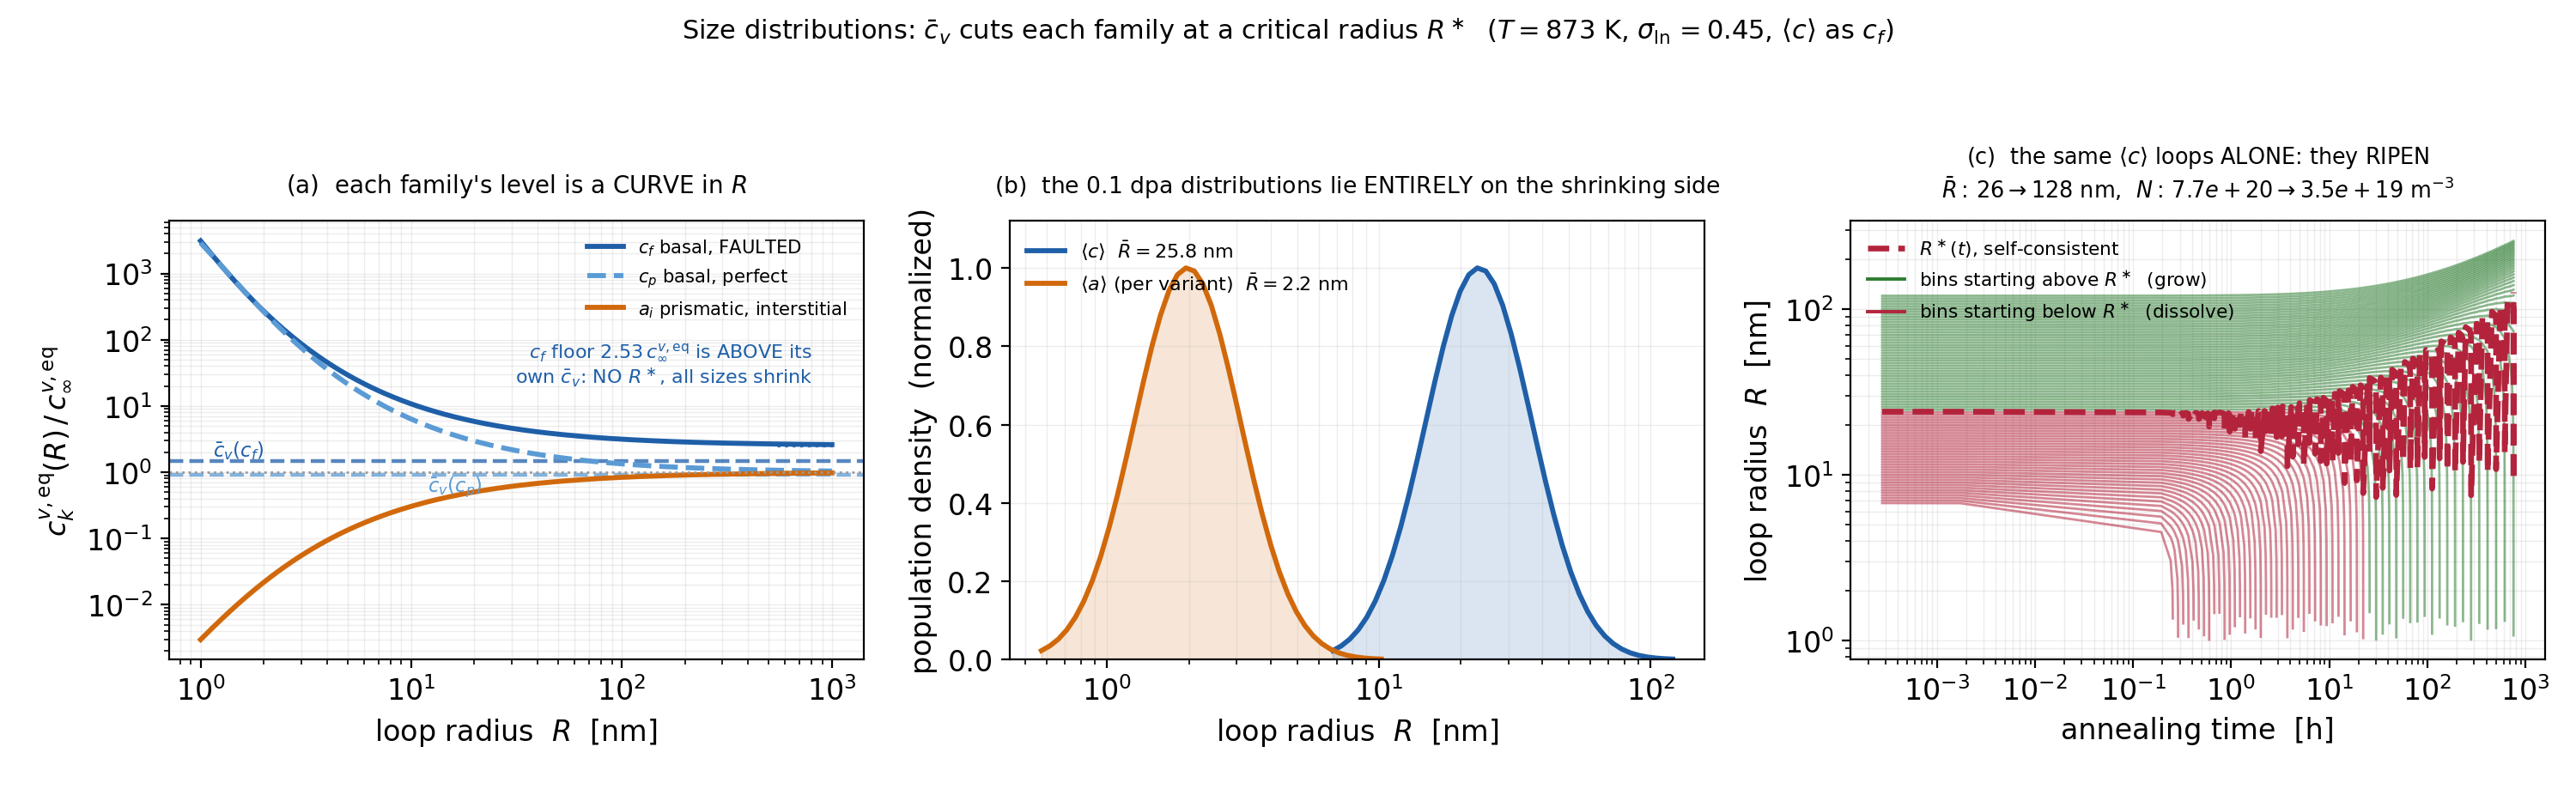
\includegraphics[width=\textwidth]{annealing_ripening.png}
\caption{What a size distribution changes. (a)~Each family's level is a curve in
$R$, drawn against the $\bar c_v$ its own mixture produces; the dotted horizontals
are the floors \cref{eq:levelfloor}. The faulted basal state's floor lies above
its own $\bar c_v$, so \cref{eq:Rstar} has no root. (b)~The reference
distributions at $0.1\,$dpa lie entirely on the shrinking side of $\bar c_v$.
(c)~The same \cloop{} population with the network and the \aloop{} loops removed,
so that $\bar c_v$ is its own: every size bin's trajectory, with the
self-consistent $R^\ast(t)$ drawn through them. Bins that start above $R^\ast$
grow at the expense of those below, which is ripening and not annealing. The
sawtooth on $R^\ast(t)$ is the bin discretization --- $\bar c_v$ is a sum over
delta functions, so every bin that dissolves steps it --- and not a feature of
the solution. The distribution width $\sigma_{\ln}=0.45$ is the one assumed
quantity in this figure. Produced by
\textttclr{...loop\_annealing\_population figure-ripening}.}
\label{fig:anneal-ripening}
\end{figure}

\paragraph{What is assumed, and what would move.} Four things, in decreasing
order of how much they matter.
\begin{enumerate}
\item \textbf{One capture efficiency must serve both sides of \cref{eq:cbar}, and
      which one is a choice worth $27\%$.} The formulation carries two that are
      not the same number: the mean-field $Z_{sk,v}$ of \cref{eq:Zsk}, from which
      \cref{eq:KL_matrix} assembles $k^2_v$, and the isolated-loop
      $Z^{\mathrm{iso}}_k$ of \cref{eq:Ziso}, which \cref{eq:popR}'s own kinetics
      use. Either may be taken --- they differ in their \emph{ratio} between
      habits, which is the only thing $\bar c_v$ sees, and on this microstructure
      that ratio differs by $1.7\times$ and $\bar c_v$ by up to $27\%$ (last two
      columns of \cref{tab:anneal-population}). \textbf{What may not be done is to
      take one in \cref{eq:cbar} and the other in \cref{eq:popR}.} The sum
      $\sum_k S_k(\bar c_v-c^{v,\mathrm{eq}}_k)$ is the net vacancy exchange with
      the matrix \emph{only} if the $S_k$ that weight it are the $S_k$ that drive
      the growth; mix them and vacancies are destroyed. That was caught by the
      conservation test above, at a factor of $85$, in a ripening run that was
      otherwise entirely plausible --- \textbf{a near-cancellation is unforgiving
      of a few per cent in its weights}, which is the same lesson
      \cref{sec:growth-laws} draws about \cref{eq:growth}. $Z^{\mathrm{iso}}_k$ is
      used throughout, because it makes \cref{eq:popR} reduce to
      \cref{eq:isolatedR} exactly in the single-component limit, which is the
      comparison this subsection is about.
\item \textbf{The mapping of the march's \cloop{} family onto $c_f$ rather than
      $c_p$.} The march carries $(\bvec\!\cdot\!\nvec)=c/2$, which is $c_f$'s
      geometry, but its loop-model kinetics carry no fault term. The choice sets
      the rung and therefore $\bar c_v$, and by \cref{eq:levelfloor} it sets
      whether a coarsening branch exists at all. Both are reported and neither is
      asserted to be the physical one; settling it is a question about the basal
      chain of \cref{sec:basal}, not about the anneal.
\item \textbf{$\bar c_v$ is spatially uniform.} \Cref{eq:cbar} is a
      zero-dimensional balance, so it is a statement about a region large compared
      with the screening length \cref{eq:screening} and small compared with the
      gradients of $n^k_{sL}(\bm x)$. It is evaluated here on the interior mean,
      which is the same restriction \cref{sec:refusal} and the hardening study
      impose, and for the same reason.
\item \textbf{The distribution width is assumed.} The model carries one mean size
      per family before \cref{sec:moments}, so $\sigma_{\ln}=0.45$ in
      \cref{fig:anneal-ripening} is an input. It re-partitions a fixed population
      --- $N$ and $\bar R$ are held exactly --- so it moves where $R^\ast$ falls
      within the distribution and not whether one exists. Carrying $q^k_{sL}$
      through the anneal, as \cref{sec:moments} does through the irradiation,
      would remove this assumption and is the natural next step.
\end{enumerate}

\subsection{Annealing a transferred discrete population}
\label{sec:anneal-discrete}

\paragraph{The setup.} Run an irradiation march to a chosen dose --- $1\,$dpa is
used below --- stop the source, convert the continuum immobile field to a discrete
loop population by \cref{sec:conversion}, and anneal that population \emph{on the
same volume}: the same mesh, the same CD nodes, the same nodal volumes
\cref{eq:mcvolumes}, the same material file. Nothing is re-staged: the staged
case is keyed on the geometry, the mesh and the material and not on the
dose grid, so an annealing run reuses the irradiation run's case
directory outright.

Four things carry over unchanged and two change.

\begin{itemize}
\item \textbf{Unchanged:} the operator split \cref{sec:split} and its ordering;
      the mobile problem, which is still the steady anisotropic
      reaction--diffusion system \cref{Eq:master_c}; the immobile ODEs at every
      node; and the conservation ledger \cref{eq:accumulators}.
\item \textbf{The source is switched off}, $G=0$, so the production integrals of
      \cref{eq:accumulators} stop accumulating and the mobile problem is driven
      \emph{only} by the emission source $\spvec S_{vL}$ of \cref{eq:Semit}. The
      sign of the whole problem inverts: under irradiation the loops are sinks
      drawing on a supersaturated pool, and under an anneal they are sources
      feeding a pool the boundary drains.
\item \textbf{The dose axis becomes a time axis.} The march advances on
      $\{\gamma_n\}$ with $\Delta t=\Delta\gamma/G$, which is undefined at $G=0$;
      the schedule is instead specified directly as a log-spaced grid in $t$,
      refined at the start where the fastest family is losing size quickest.
\end{itemize}

\paragraph{The split is more comfortable here, not less.} \Cref{sec:scales} rests
the quasi-steady approximation on the mobile field equilibrating fast against the
immobile evolution. Removing the source slows the immobile evolution --- there is
no production to drive it, only the residual supersaturation of
\cref{tab:anneal-binding} --- so the separation widens and the fast-solve cadence
\textttclr{fem\_every} can be relaxed. One caution runs the other way and is
specific to annealing: the emission source \cref{eq:Semit} depends on
$c^{v,\mathrm{eq}}_{sk}(\bar m^k)$, which is \emph{exponential} in the loop size,
so a family close to the floor changes its own source term by a factor of $e$ over
a size change of $k_BT/(\partial^2E_k/\partial m^2)$. The splitting error of
\cref{sec:splitting} is still first order in the fast-solve spacing, but the
coefficient grows through the anneal rather than shrinking, and the cadence should
be tightened at the end where it can be loosened at the start.

\paragraph{The boundary condition is not a free choice.} On a domain with
Dirichlet faces the emitted vacancies leave, the pool stays near
$c^{v,\mathrm{eq}}_\infty$, and the population anneals to extinction --- which is
the case \cref{sec:anneal-isolated} idealizes. On a \emph{fully periodic} cell
nothing leaves; the total vacancy content is conserved exactly, so the loops
cannot all disappear, and the calculation converges instead on an Ostwald
ripening steady state in which large loops grow at the expense of small ones at
constant total content. Both are physical and they are different experiments: a
thin TEM foil or a fine-grained specimen is the first, a well-annealed
single-crystal interior is closer to the second. \textbf{\textttclr{BOUNDARY['periodic\_face\_ids']} therefore selects
which annealing experiment is being simulated}, and an empty list --- the default --- is the extinction case.

\paragraph{Option 1: annealing through the growth equation.} Every loop is
advanced by its own copy of \cref{eq:isolatedR}, or of
\cref{eq:romA,eq:romB} where the outline is allowed to be elliptical, with two
substitutions that acknowledge the loop is no longer alone. The ambient field
$c^{v}$ becomes the continuum field $c^{v}_{\mathcal C}(\bm x_\ell)$ at the loop's
center plus the lagged monopole sum over the neighbors inside the cutoff
\cref{eq:cutoff}, exactly as in \cref{sec:ellipse-rom}; and $Z^{\mathrm{iso}}_k$
returns to $Z_{sk,v}$ of \cref{eq:Zsk} wherever the population is dense enough
for a bias to mean anything. The cost is $O(N_{\mathrm{loop}})$ per step plus the
neighbor sum, the loops decouple, and forward Euler is adequate for the same
reason \cref{sec:climb-status} gives.

\textbf{Its one free parameter loses its default.} $L_{\mathrm{cap}}$ in
\cref{eq:romA,eq:romB} is set to the screening length \cref{eq:screening}, on the
argument that a loop draws on the medium out to the distance at which some other
sink intercepts the defect first. That argument survives an anneal; the
\emph{number} does not survive the loop shrinking. \Cref{eq:screening} is a
property of the surroundings and is essentially fixed here --- see below --- while
$R^k_{sL}$ falls to the floor, so $L_s/R$ runs from about $1$ at the transfer
state to $73$ at $R_{\min}$ on the reference case. Once $L_s\gg R$ the gradient
feeding the line develops over the loop's own size and not over $L_s$: the outer
cutoff of the capture problem is set by the sink itself, which is what
\cref{eq:Ziso} states in its logarithm, and $L_{\mathrm{cap}}$ must cross over
from $L_s$ to $O(R^k_{sL})$. \textbf{An
annealing run that keeps $L_{\mathrm{cap}}=L_s$ throughout under-reads the
late-time shrinkage rate by that same ratio}, and the error is largest exactly
where the loops are disappearing --- which is the part of the trajectory an
annealing experiment measures.

\paragraph{Option 2: annealing through the Green's-function solve.} The
boundary-integral construction of \cref{sec:bim-climb} is used unchanged. Neither
the kernel \cref{eq:Gkernel} nor the assembly \cref{eq:Kclimb,eq:Fclimb} contains
anything that assumes a growing loop: the driving supersaturation
\cref{eq:cline} simply changes sign, the climb velocities $v^m_\nu$ come out
negative, and $c^m_{\mathcal D}$ of \cref{eq:cDD} is a positive hump around each
loop rather than a depletion halo. What this buys over Option~1 is the one
mechanism a monopole cannot carry: \textbf{a shrinking loop's vacancies are
re-absorbed preferentially by its nearest neighbors}, which slows the anneal
locally and by an amount that depends on where the neighbors are. A mean field
carries the average of that through $k^2_m$ and cannot carry its variance, and it
is precisely at the small separations where the effect is largest that the
average is least representative.

\textbf{The cutoff survives an anneal, and the reason is the dislocation
network.} \Cref{eq:cutoff} sets $R_{\mathrm{cut}}=n_LL_s$ with $n_L=4$, and the
obvious worry is that $L_s$ runs away as the loops vanish, taking the pair count
with it. It does not, because the loops are not the only sink: $k^2_m$ in
\cref{eq:KL_matrix} carries the network density $\rho_N$, which an anneal of the
loop population does not remove. On the reference case at $10\,$dpa
$L_s=59.0\,$nm, i.e.\ $k^2_m=2.87\times10^{14}\,$m$^{-2}$, of which
$\rho_N=1.88\times10^{14}\,$m$^{-2}$ is $65\%$; removing the loops entirely
therefore takes $L_s$ only to $\rho_N^{-1/2}=72.9\,$nm, a rise of $24\%$, and
$R_{\mathrm{cut}}$ from $236$ to $292\,$nm. \textbf{The pair count per loop grows
by at most $(1.24)^3\simeq1.9$ while the loop count falls to zero}, so the cost
of Option~2 falls monotonically through the anneal. The same bound is what keeps
the truncation \emph{legitimate}: the justification for cutting the sum is that
$k^2_m$ already carries the mean-field response, and $k^2_m$ retains two thirds
of its magnitude no matter how completely the loops anneal. Both statements fail
together in a crystal whose network has also recovered, and that is the case in
which \cref{eq:cutoff} must be re-derived rather than re-used.

\paragraph{The selection rule runs backwards during an anneal, and that is the
operational result.} \Cref{eq:selectors} defines the two independent selectors,
and both fall as the loops shrink --- but by wildly different amounts, and it is
the disparity rather than the direction that decides the run. With the loop
number fixed $d_k$ is fixed, the loops' own contribution to $k^2_m$ is
proportional to $\rho^k_{sL}=2\pi R^k_{sL}n^k_{sL}$ and so to $R^k_{sL}$, and the
network's contribution is not, so
\begin{equation}
  \Theta_k=\frac{2R^k_{sL}}{d_k}\;\propto\;R^k_{sL}\;\longrightarrow\;0,
  \qquad
  \Xi_k=d_k\sqrt{k^2_{\mathcal N}+\varkappa R^k_{sL}}
   \;\longrightarrow\;d_k\sqrt{k^2_{\mathcal N}} ,
  \label{eq:annealselectors}
\end{equation}
with $k^2_{\mathcal N}$ everything in \cref{eq:KL_matrix} that is not the
annealing family. \textbf{$\Theta_k$ goes to zero and $\Xi_k$ barely moves.} On
the reference case $\Xi_k$ for the \cloop{} family falls only from $1.856$ to
$1.501$, by the factor $\sqrt{\rho_N/k^2_m}=0.809$, and stays inside the
merged-halo column of \cref{tab:climb-selection} for the whole anneal. So the
family crosses \emph{one} cell boundary and not two: it leaves the crowded row
and never leaves the merged-halo column, which is exactly the trajectory
\cref{tab:anneal-options} is built around. What it does not do is cross it
early.

The reference \cloop{} family enters at $R=57.6\,$nm and $d_k=109.5\,$nm, i.e.\
$\Theta_k=1.05$, in the lower-left cell of \cref{tab:climb-selection} where its
loops overlap on average. $\Theta_k$ falls below $0.5$ only at $R=27.4\,$nm, and
integrating \cref{eq:isolatedR} for the faulted state gives that at $22.3\,$h of
a $29.5\,$h anneal-out at $873\,$K, and at $35.5\,$min of $47.4\,$min at
$973\,$K. \textbf{Three quarters of the anneal is spent in the crowded regime},
because $\dot R$ is smallest when the loop is largest, and the population spends
most of its life near the size it started at. So the representation must be
switched \emph{during} the run, on $\Theta_k$ evaluated from the discrete
population itself, and the switch pays for only the last quarter.

\begin{table}[htbp]
\centering
\small
\caption{The two annealing constructions. Both are exact statements of
\cref{eq:vn-common}; they differ in what supplies the concentration at the line,
which is the same distinction \cref{sec:climb-common} draws under irradiation.
The last row is the one that decides a run.}
\label{tab:anneal-options}
\begin{tabularx}{\textwidth}{@{}p{3.3cm} X X@{}}
\toprule
 & Option 1 --- growth equation & Option 2 --- Green's functions\\
\midrule
unknowns per loop & $1$ (circular) or $2$ (elliptical),
  \cref{eq:isolatedR,eq:romA,eq:romB} &
  $N_{\mathrm{side}}\times4$ climb velocities, \cref{eq:climbsystem}\\
\addlinespace
field at the line & continuum $c^{v}_{\mathcal C}$ plus a lagged monopole sum &
  solved: $c^{v}_{\mathcal D}$ from \cref{eq:cDD}, linear in the velocities\\
\addlinespace
capillarity & inside $c^{v,\mathrm{eq}}_{sk}$, \cref{eq:dEdmstress}, with the
  fault term & from the network's own stress, \cref{eq:cline}; the fault term
  must be added to it\\
\addlinespace
cost & $O(N_{\mathrm{loop}})$, falling through the anneal &
  $O(N_{\mathrm{seg}}^2)$ inside $R_{\mathrm{cut}}=n_LL_s$, and
  $R_{\mathrm{cut}}$ \emph{grows} through the anneal\\
\addlinespace
misses & neighbor re-absorption beyond the monopole; contact coalescence;
  departure from an ellipse & nothing structural; it is the cost that limits it\\
\addlinespace
\textbf{when to use} & $\Theta_k\lesssim0.5$, i.e.\ the last quarter of the
  anneal for the reference \cloop{} population &
  $\Theta_k\gtrsim0.5$, i.e.\ the first three quarters\\
\bottomrule
\end{tabularx}
\end{table}

\paragraph{Losing loops, and why this is the calibration experiment for
\cref{sec:moments}.} In the continuum representation a family loses loops through
the floor current \cref{eq:floorcurrent}, which is an integral of the assumed
log-normal \cref{eq:closure} below $m_{\min}$ --- a closure, evaluated from two
moments. In the discrete representation a loop reaching $R_{\min}$ is deleted and
its remaining defects are returned to the mobile pool, one loop at a time, by
counting. \textbf{The two are the same physical process computed two entirely
different ways, and an anneal is the only regime in which the process is the
dominant one.} Running both on the same transferred state therefore measures the
closure directly: $n^k_{sL}(t)$ from the continuum against the surviving loop
count from the discrete population, on the same volume, with no fitted quantity
between them. Two features make the comparison sharp rather than merely
suggestive.

\begin{itemize}
\item \textbf{The signature is qualitative.} \Cref{sec:basal} noted that the
      two-moment model gives constant density and falling mean size under a pure
      anneal, where experiment reports density \emph{falling} and the surviving
      mean size \emph{rising}. A discrete population reproduces the experimental
      signature by construction --- the smallest loops are the ones that reach the
      floor --- so the test is whether \cref{eq:floorcurrent} reproduces it too,
      and by how much.
\item \textbf{The dispersion is transferred, not assumed.} \Cref{sec:sizesampling}
      draws each loop's size from the same log-normal the closure integrates, so
      at $t=0$ the two representations agree on the distribution exactly. Any
      subsequent divergence is the closure failing to track a distribution that
      \cref{eq:isolatedR} is reshaping --- and it will reshape it, because
      $\dot R$ is size-dependent and, by \cref{eq:annealasym}, size-dependent
      differently for the two basal states.
\end{itemize}

\paragraph{Conservation during an anneal is a stronger check than during
irradiation.} The ledger \cref{eq:accumulators} loses its largest term when the
source is switched off, so what remains is a balance among quantities of
comparable size:
\begin{equation}
  \underbrace{\Delta\!\left(\textstyle\sum_{(s,k)}\eta_s\,c^k_{sL}\right)}
             _{\text{stored, falling}}
  +\underbrace{\Delta\!\left(\textstyle\sum_m|m|\,c^m\right)}_{\text{mobile}}
  +\underbrace{\int_0^t\!\!\oint_{\partial\Omega}\bm J\!\cdot\!\nvec\,
     \mathrm dA\,\mathrm dt'}_{\text{grain boundary}}
  \;=\;0 .
  \label{eq:annealledger}
\end{equation}
Under irradiation the boundary term is $71\%$ of cumulative production and the
stored term is $0.1\%$ of it (\cref{sec:conservation}), so closure tests the
large channels and says almost nothing about the small one. In an anneal the
stored term \emph{is} the source, and \cref{eq:annealledger} becomes a direct
test of whether every vacancy that left a loop was accounted for --- including the
ones returned by loops deleted at the floor, which is the step most likely to lose
them. On a periodic cell the boundary term is identically zero and
\cref{eq:annealledger} reduces to a two-term conservation statement that must
hold to solver tolerance, which is the cheapest available regression test on the
whole annealing path.

\paragraph{What is implemented.} \Cref{eq:isolatedR,eq:Ebstress,eq:emitrate} and
every number in \cref{tab:anneal-binding,tab:anneal-emission,tab:anneal-lifetime}
are produced by \textttclr{dislocluster\_code.studies.loop\_annealing}, which
reads its constants from the material file and is verified against the closed
forms of \cref{sec:loopchar}. It is a standalone evaluation of this section's
equations and does not run a march. The march-level annealing path requires, in
order: the computed binding energy in place of the $5\,$eV surrogate
(\cref{sec:anneal-emission}), a $G=0$ schedule specified in time rather than
dose, and the $\Theta_k$-triggered switch between the two constructions of
\cref{tab:anneal-options}. The first is already step~3 of
\cref{sec:plan-phase2}; the other two are steps~14 and~16 of
\cref{sec:plan-anneal}. \textbf{A fourth requirement is not visible from the
formulation and was found in the assembled system}: \cref{Eq:master_c}'s emission
source $\spvec S_{vL}$, \cref{eq:Semit}, has no counterpart in the mobile solve at
all, which under irradiation is a small correction and under an anneal is the
entire drive. It is step~13, it comes before the other two, and
\cref{eq:cbar} is its acceptance test. The test cases for annealing a
\emph{distribution} --- in both representations, which is the comparison this
subsection argues is the calibration experiment for \cref{sec:moments} --- are
\cref{tab:anneal-tests}.

\section{Macroscopic Observables and Mechanics Coupling}
\label{sec:observables-mech}

Three quantities are asked of this model by anyone who has to use it: irradiation
\emph{growth}, irradiation \emph{creep}, and radiation \emph{hardening}. This
section states how each is computed, and it must state it twice, because past
$d_{\mathrm{coarsen}}$ the loop population exists in two representations at once
and no observable may be taken from one of them alone.

\textbf{The three observables are two objects.} Growth and creep are the same
tensor --- the plastic distortion carried by the loop population --- read at two
different times: growth is its accumulated value under no applied load, creep the
rate of its deviator under one. Hardening is not a distortion at all but a
threshold stress, and it is nonlinear in the population, which is why it composes
differently from the other two.

\textbf{The population is split, and the split is not a detail.} From
\cref{sec:trigger}, a family that crosses $\phi^\ast$ has the fraction
$f_{\mathrm{kept}}$ of its defects converted to discrete loops while
$1-f_{\mathrm{kept}}$ stays in the continuum, and \cref{sec:refusal} measures $f_{\mathrm{kept}}$
falling from $0.99$ to below $0.01$ across a decade of dose on a $500\,$nm domain.
An observable evaluated on the continuum fields alone is therefore too small by
$f_{\mathrm{kept}}$, and one evaluated on the pre-transfer fields plus the discrete
population is too large by the same factor. \Cref{sec:obs-compose} states the
composition rules; they are not the same rule for all three observables.

\subsection{The continuum representation}
\label{sec:obs-continuum}

\paragraph{One tensor underlies both growth and creep.} A loop of family $(s,k)$
is a platelet: an area $A_\ell$ of habit plane $\hat{\bm n}_k$ across which the
crystal has gained or lost one layer of atoms of thickness
$(\bvec\!\cdot\!\nvec)_k$. Its contribution to the plastic distortion of a volume
$V$ is $\eta_s A_\ell(\bvec\!\cdot\!\nvec)_k\,\hat{\bm n}_k\!\otimes\!\hat{\bm
n}_k/V$, and the platelet volume per unit crystal volume summed over a family is
by construction its stored content, $\sum_\ell A_\ell(\bvec\!\cdot\!\nvec)_k/V
=c^k_{sL}$. Hence
\begin{equation}
  \bm\beta^{P}=\sum_{(s,k)\in\mathcal F}\eta_s\,\Upsilon_{h(k)}\;c^k_{sL}\;
    \hat{\bm n}_k\!\otimes\!\hat{\bm n}_k ,
  \label{eq:betaP}
\end{equation}
with $\eta_s=\pm1$ the character sign of \cref{sec:families}. \textbf{The content
fields are the plastic distortion, up to one factor per habit.} $\Upsilon_{h(k)}$
is that factor: it is unity if a stored defect displaces exactly $\Omega$, and
departs from unity only by the ratio of the defect's relaxation volume to
$\Omega$. It is written $\Upsilon$ and not $A$ deliberately --- $A_{h(k)}(p_m)$ in
\cref{eq:Afactors} is the Woo orientation factor, an unrelated quantity, and the
two were carried under one symbol in an earlier revision of this document.

\Cref{eq:betaP} is the only constitutive statement on the continuum side. Growth
and creep are two readings of it.

\paragraph{Growth.} At zero applied stress the variants are equally populated and
\cref{eq:betaP} is diagonal in the crystal frame. Its prismatic and basal
components are
\begin{equation}
  \varepsilon_a=\Upsilon_a\!\!\sum_{(i,a_k)}\!\!c^{a_k}_{iL}
    \;-\;\Upsilon_a\!\!\sum_{(v,a_k)}\!\!c^{a_k}_{vL},
  \qquad
  \varepsilon_c=-\Upsilon_c\left(c^{c_f}_{vL}+c^{c_p}_{vL}
        +\zeta_{c_0}\,c^{c_0}_{vL}\right),
  \label{eq:strain}
\end{equation}
the prismatic vacancy families entering with the opposite sign to their
interstitial counterparts, which is the direct macroscopic consequence of
carrying both characters --- and the reason the coexistence question of
\cref{sec:coexist} is an observable question and not only a microstructural one.
$\zeta_{c_0}\simeq\tfrac13$ is the fraction of the pyramid's nearly isotropic
relaxation volume that resolves on $[0001]$, against unity for the two planar
states. \textbf{That single coefficient is where the incubation appears in an
observable}: while the basal vacancies sit in $c_0$ they contribute a third of
their share to $\varepsilon_c$, and the accelerated $c$-axis growth begins only as
\cref{eq:transfer} moves them onto planes.

\paragraph{Creep.} Under load the variants are no longer equally populated, and
what an experiment measures is the deviator of \cref{eq:betaP} evolving in time,
\begin{equation}
  \dot{\bm\varepsilon}^{\mathrm{creep}}
   = \sum_{(s,k)\in\mathcal F}\eta_s\,\Upsilon_{h(k)}\,
     \dot c^{k}_{sL}\,\left(\hat{\bm n}_k\otimes\hat{\bm n}_k
       -\tfrac13\mathbb I\right),
  \label{eq:creep}
\end{equation}
a tensor rather than the scalar an alignment fraction could produce. \textbf{The
variant resolution of \cref{eq:families} is what makes \cref{eq:creep} possible at
all}: with the three prismatic variants lumped there is no imbalance to take a
deviator of, and SIPA appears only as a scalar bias. The stress enters through
the variant weights and the SIPA bracket of \cref{eq:Zsk}, so nothing in
\cref{eq:creep} is fitted to creep data.

The trace of \cref{eq:betaP} is not discarded: it is the swelling, and it is
small here because the two characters store nearly equal numbers of atoms
(\cref{sec:conservation}), not because either term is small.

\paragraph{Where it enters the solver.} The rate form is supplied per point as
$\bm L^{P}=\sum_X\dot c^X\,(\hat{\bm n}_X\!\otimes\!\hat{\bm n}_X)$, differenced
across the immobile step from the endpoint states rather than differentiated ---
the states are what the slow step returns, and a one-sided difference over the
substep is consistent with the operator split of \cref{sec:solution} to the same
order as the split itself.

\paragraph{Hardening.} Hardening is not a distortion and does not follow from
\cref{eq:betaP}. Each family is an obstacle population of number density
$N_k=n^k_{sL}/\Omega$ and obstacle \emph{diameter} $d_k=2R^k_{sL}$, and the
dispersed-barrier law gives
\begin{equation}
  \Delta\tau_k=\alpha_k\,\mu\,b\,\sqrt{N_kd_k},
  \qquad
  \Delta\tau_{SR}=\Bigl[\sum_k\Delta\tau_k^{2}\Bigr]^{1/2},
  \qquad
  \Delta\tau_{LR}=\alpha_{LR}\,\mu\,b\,\sqrt{\rho_N},
  \label{eq:dispersed}
\end{equation}
the short-range contributions adding in quadrature and the long-range network
term separately, and the yield increment following by the Taylor factor $M$,
\begin{equation}
  \Delta\sigma_y=M\left(\Delta\tau_{SR}+\Delta\tau_{LR}\right).
  \label{eq:taylor}
\end{equation}
\textbf{\Cref{eq:taylor} multiplies by $M$; an earlier revision of this document
divided by it.} The Taylor factor converts a resolved shear stress into the
macroscopic stress that produces it, $\sigma=M\tau$ with $M\simeq3$, so dividing
understates the yield increment by an order of magnitude. The implementation has
always multiplied.

\textbf{Neither $\alpha_k$ nor $M$ is computed by this model}, and neither has a
default that would be distinguishable in the output from a fitted one. Both must
be stated whenever a hardening number is quoted. \Cref{sec:obs-discrete} is where
$\alpha_k$ comes from.

\subsection{The discrete representation}
\label{sec:obs-discrete}

Once a family is discrete, none of \cref{eq:betaP,eq:dispersed} is needed for it:
the mechanics machinery that the dislocation code already carries computes the
same observables without a constitutive step, and the two subsections differ in
exactly that.

\paragraph{Growth and creep are measured, not modelled.} The dislocation code
accumulates the plastic distortion of the network as its segments move, and
writes the full tensor and its rate at every step,
\begin{equation}
  \bm\beta^{P}_{\mathcal D}
   =\frac{1}{V}\sum_{\lambda}\;\frac{1}{2}\bigl(\bvec_\lambda\otimes\bm A_\lambda
        +\bm A_\lambda\otimes\bvec_\lambda\bigr),
  \qquad
  \bm A_\lambda=\text{area swept by segment }\lambda,
  \label{eq:betaPdisc}
\end{equation}
alongside $\dot{\bm\beta}^{P}_{\mathcal D}$, together with $\operatorname{tr}$ and
$\|\cdot\|$ of each. Three things follow, and they are the reason to want the
discrete representation for an observable at all.

\begin{itemize}
\item \textbf{No strain factor appears.} \Cref{eq:betaPdisc} is a sum over the
      segments that actually moved, with their actual Burgers vectors; there is
      no $\Upsilon_{h(k)}$ to assign and no habit-plane idealization. Comparing
      it against \cref{eq:betaP} on the same population is therefore a
      \emph{measurement} of $\Upsilon_{h(k)}$, which is the one clean route to a
      quantity the continuum side has to assume.
\item \textbf{Climb and glide separate by the trace.} A climbing prismatic loop
      has $\bvec\parallel\hat{\bm n}$ and contributes to
      $\operatorname{tr}\bm\beta^{P}$; glide is volume-conserving and does not. So
      the trace isolates the irradiation-driven part from the deformation-driven
      part with no tagging of segments.
\item \textbf{It is a rate, natively.} $\dot{\bm\beta}^{P}$ is what the creep
      measurement wants and is written directly, where the continuum side must
      difference \cref{eq:betaP} across a substep.
\end{itemize}

The cost is that \cref{eq:betaPdisc} is only as good as the climb velocities
feeding it, which is the accuracy question \cref{sec:bim-climb} settles through
the cutoff convergence --- the climb strain rate is precisely the quantity that
sweep is flat in.

\paragraph{Hardening is measured by loading the cell.} The discrete route does
not evaluate \cref{eq:dispersed}; it rebuilds the interior population as loops in a
periodic cell, loads it, and reads the critical resolved shear stress off the
response. Three routes are staged and they are not alternatives of equal cost:

\begin{center}\small
\begin{tabularx}{\textwidth}{@{}l l X@{}}
\toprule
route & what it does & cost and role \\
\midrule
A & stress ramp on a frozen obstacle field; $\Delta\tau$ read directly &
the reference measurement, but affordable only at selected doses \\
C & \cref{eq:dispersed} with $\alpha_k$ \emph{fitted on route A} &
free at every dose once $\alpha_k$ is known --- this is how the continuum side
acquires its $\alpha_k$ \\
D & the same cell seeded by density rather than per-loop export &
the smoke test, not a measurement \\
\bottomrule
\end{tabularx}
\end{center}

Route B --- the full stress--strain curve at imposed strain rate --- is days per
dose and is deliberately not staged. \textbf{The relationship between routes A
and C is the whole point of the pairing}: A is the only thing here that measures
$\alpha_k$, and C is what makes the measurement usable at doses A cannot reach.

Two properties of the measurement must be quoted with any number it produces.
\textbf{The criterion is an offset}, the stress at which the plastic shear first
reaches a stated value; an irradiated cell creeps below its breakaway stress, so
the number depends on the offset and the offset is a choice, not a property of
the material. And \textbf{the loops are frozen}: they are inserted as sessile
loops with no climb solver attached, so they neither absorb nor are cut, and
nothing channels. That is the largest modeling assumption in the measurement and
it biases hardening high as strain accumulates.

\paragraph{Composing the two representations.}
\label{sec:obs-compose}
Past $d_{\mathrm{coarsen}}$ both representations hold part of the same family, and
the rule for combining them is different for the distortion observables and for
hardening. It follows from whether the observable is linear in the population.

\begin{table}[htbp]
\centering
\small
\caption{How an observable is composed when a family is split between the two
representations, with $f_{\mathrm{kept}}$ the discrete share of
\cref{sec:refusal}. The continuum fields used must always be the
\emph{post}-transfer ones, which \cref{sec:trigger} has already scaled by
$1-f_{\mathrm{kept}}$.}
\label{tab:obs-compose}
\begin{tabularx}{\textwidth}{@{}l l X@{}}
\toprule
observable & composition & why \\
\midrule
growth $\bm\beta^{P}$ &
$\bm\beta^{P}_{\mathcal C}+\bm\beta^{P}_{\mathcal D}$, \textbf{linear} &
\Cref{eq:betaP} is linear in $c^k_{sL}$ and \cref{eq:betaPdisc} is a sum over
segments; the two partition the same stored content. \\
\addlinespace
creep $\dot{\bm\varepsilon}$ &
$\dot{\bm\varepsilon}_{\mathcal C}+\dot{\bm\varepsilon}_{\mathcal D}$,
\textbf{linear} &
Same argument on the rate. Both must be expressed in the same frame and unit
system first; the discrete side is written in the code's own $c_s/b$. \\
\addlinespace
hardening $\Delta\tau$ &
$\bigl[\Delta\tau_{\mathcal C}^{2}+\Delta\tau_{\mathcal D}^{2}\bigr]^{1/2}$,
\textbf{root-sum-square} &
$\Delta\tau\propto\sqrt N$, so linear addition over-counts. See
\cref{eq:rsssplit}. \\
\addlinespace
sink strength $k^{2}_m$ &
continuum part only, \textbf{plus} \cref{eq:kdiscrete} &
The transferred loops were removed from \cref{eq:KL_matrix} at the transfer;
adding them back is what \cref{sec:climb-selection} is about. \\
\bottomrule
\end{tabularx}
\end{table}

\textbf{Why root-sum-square is not an approximation here.} Split one family into a
continuum part of density $N_{\mathcal C}$ and a discrete part $N_{\mathcal D}$ at
the same obstacle diameter $d$ and strength $\alpha$. Then
\begin{equation}
  \sqrt{\Delta\tau_{\mathcal C}^{2}+\Delta\tau_{\mathcal D}^{2}}
   =\alpha\mu b\sqrt{\bigl(N_{\mathcal C}+N_{\mathcal D}\bigr)d}
   =\Delta\tau\bigl[N_{\mathcal C}+N_{\mathcal D}\bigr],
  \label{eq:rsssplit}
\end{equation}
that is, quadrature over the two pieces reproduces \emph{exactly} the single
population they were cut from. Linear addition would instead give
$\alpha\mu b(\sqrt{N_{\mathcal C}d}+\sqrt{N_{\mathcal D}d})$, which overstates the
result by up to $\sqrt2$ at an even split. \Cref{eq:rsssplit} is the same rule
\cref{eq:dispersed} already applies across families, and it is what makes a split
family harmless \emph{provided both pieces are scored by the same law}.

\textbf{That proviso is where the care is needed.} A route-A measurement of the
discrete part is not a $\Delta\tau_k$ computed from \cref{eq:dispersed}: it is a
response of a cell containing those loops, and it already includes whatever
$\alpha$ they actually have. Combining a measured $\Delta\tau_{\mathcal D}$ with a
law-derived $\Delta\tau_{\mathcal C}$ by \cref{eq:rsssplit} therefore assumes the
continuum remainder has the same obstacle strength as the exported loops --- which
is the assumption route~C exists to test and not one to make silently. The clean
procedure is the one the routes were built for: fit $\alpha_k$ on route A at a
dose where the transfer is feasible, then score \emph{both} pieces with
\cref{eq:dispersed}.

\textbf{Three failure modes, all of them silent.} A transfer leaves no marker in
the fields it reduced, so each of these produces a plausible number:

\begin{enumerate}
\item \textbf{Using the pre-transfer continuum field.} The observable is then too
      large by exactly $f_{\mathrm{kept}}$ in the distortion channels --- a factor
      of two at $f_{\mathrm{kept}}=0.5$, and at $0.99$ it is a doubling.
\item \textbf{Reporting a domain mean rather than an interior mean.} The boundary
      shell carries up to $99.8\%$ of the \aloop{} density
      (\cref{sec:refusal}), so a domain mean of any loop observable measures the
      shell. Every number in \cref{sec:obs-discrete} is an interior mean, by the
      same innermost-quartile rule the transfer itself uses.
\item \textbf{Counting the network twice.} The loop--network channel of
      \cref{eq:coal} feeds absorbed loop line length into $\rho_N$, and
      $\rho_N$ then appears in $\Delta\tau_{LR}$ of \cref{eq:dispersed}. Once a
      family is discrete, that absorption happens in the dislocation code
      instead, and a $\rho_N$ still being advanced by \cref{eq:coal} for the
      transferred share double counts it.
\end{enumerate}

\textbf{The refused share is misplaced, not lost.} One further caution follows
from \cref{sec:climb-selection}: refusal is a spatial criterion --- loops are
refused for being near a face --- while the defects they carried are returned to
the continuum by a single scalar applied at every node alike. The atom balance
closes, so \cref{eq:betaP} evaluated over the whole domain is right; a
\emph{locally} resolved observable in the boundary shell is not.

\subsection{Mechanics observables options}
\label{sec:obs-options}

\Cref{sec:obs-continuum,sec:obs-discrete} describe two representations. They do
not by themselves say which to use, and that is a separate decision with three
answers, because a representation is not the same thing as a \emph{route to a
number}. \Cref{tab:obs-options} states the three and what each costs; the rest of
this subsection is why the third exists.

\begin{table}[htbp]
\centering
\small
\caption{The three routes to a mechanics observable. ``Assumed'' means a
coefficient the route cannot itself determine and which must therefore be quoted
with any number it produces.}
\label{tab:obs-options}
\begin{tabularx}{\textwidth}{@{}l X X l@{}}
\toprule
Route & Measured & Assumed & Dose range \\
\midrule
(1) continuum &
nothing --- everything follows from $c^k_{sL}$, $n^k_{sL}$ &
$\Upsilon_{h(k)}$, $\alpha_k$, $\alpha_{LR}$, $M$ &
all \\
\addlinespace
(2) discrete &
$\bm\beta^{P}$, $\dot{\bm\beta}^{P}$, $\Delta\tau$ &
$M$ only &
$d\lesssim d_{\mathrm{feas}}$ \\
\addlinespace
(3) hybrid &
$\Upsilon_{h(k)}$, $\alpha_k$ at the calibration doses &
$M$; that $\alpha_k$, $\Upsilon_{h(k)}$ carry over in dose &
all \\
\bottomrule
\end{tabularx}
\end{table}

\paragraph{(1) Continuum.} Evaluate \cref{eq:betaP,eq:strain,eq:creep,eq:dispersed,eq:taylor}
on the fields the march already carries. No transfer is performed, no
dislocation calculation is run, and the cost is a post-processing pass over the
stored snapshots.

Its strength is that it is defined at every dose, including doses at which
\cref{sec:trigger-window} shows no transfer is possible at all, and it is the
only route with that property. Its weakness is the ``assumed'' column:
$\Upsilon_{h(k)}$ converts stored content to strain, and $\alpha_k$ converts an
obstacle population to a stress, and \textbf{neither is computed anywhere in the
continuum model}. A continuum hardening curve is therefore a statement about
$N_k(d)$ and $d_k(d)$ with the constitutive step supplied from outside.

There is a second and subtler limitation. Past $d_{\mathrm{coarsen}}$ the
mean-field treatment of coalescence is by construction no longer reliable
(\cref{sec:dcoarsen}), and $N_k$ and $R^k_{sL}$ are exactly the quantities that
treatment sets. \textbf{So route~1 is not merely unvalidated above
$d_{\mathrm{coarsen}}$; its inputs are the ones the detector has flagged.} That
is a sharper objection than the missing coefficients, because no amount of
external calibration repairs it.

\paragraph{(2) Discrete.} Convert the population to loops at selected doses
(\cref{sec:conversion}) and compute the observables entirely within the
dislocation code: $\bm\beta^{P}$ and $\dot{\bm\beta}^{P}$ from
\cref{eq:betaPdisc}, and $\Delta\tau$ by loading the cell. Nothing is assumed but
the Taylor factor, which is a polycrystal-averaging statement and not a property
of this model at all.

\textbf{The binding constraint is feasibility, not cost.} \Cref{sec:refusal}
measures the accepted defect share $f_{\mathrm{kept}}$ falling from $0.99$ at
$10^{-2}\,$dpa to $0.0096$ at $1\,$dpa on a $500\,$nm domain, because the
\cloop{} radius outgrows the cell. Write $d_{\mathrm{feas}}$ for the dose at
which $f_{\mathrm{kept}}$ leaves unity. Then:
\begin{equation}
  d_{\mathrm{feas}}\;\gtrsim\;d_{\mathrm{coarsen}}
  \quad\text{is required for route 2 to be available where it is needed,}
  \label{eq:feaswindow}
\end{equation}
and on the reference geometry the two are $\simeq0.1\,$dpa and $0.104$--$0.127\,$dpa
respectively --- \textbf{they coincide, and the window in which route~2 is both
necessary and possible is a factor of two or three in dose.} Above it a ``fully
discrete'' calculation is not expensive, it is unavailable: the population that
would carry the observable is the part the crystal refuses.

Two further properties must be quoted with any route-2 number. The exported
loops are inserted sessile with no climb solver attached, so they neither absorb
nor are cut and nothing channels, which biases hardening high as strain
accumulates; and the yield point is an offset criterion, so the number depends on
an offset that is a choice.

\paragraph{(3) Hybrid.} Use route~2 where it is feasible to \emph{measure the
coefficients route~1 assumes}, then use route~1 with those coefficients
everywhere, adding the discrete contribution wherever a transfer has actually
been performed. Concretely:

\begin{enumerate}
\item \textbf{Calibrate small.} At one or more doses below $d_{\mathrm{feas}}$,
      where $f_{\mathrm{kept}}\simeq1$ and the cell can hold the population,
      export and run. Two coefficients come out, and they are the two route~1
      cannot produce:
      \begin{itemize}
      \item $\alpha_k$, by fitting \cref{eq:dispersed} to the measured
            $\Delta\tau$ --- this is exactly the route~A/route~C pairing of
            \cref{sec:obs-discrete};
      \item $\Upsilon_{h(k)}$, by comparing $\bm\beta^{P}_{\mathcal D}$ of
            \cref{eq:betaPdisc} against \cref{eq:betaP} evaluated on the same
            population. \textbf{The discrete side carries no strain factor}, so
            the ratio of the two \emph{is} the factor.
      \end{itemize}
      A small cell suffices, because both coefficients are properties of the
      obstacle and the defect, not of the domain.
\item \textbf{Compose past the coarsening dose.} Where a transfer has fired, the
      family is split and \cref{tab:obs-compose} applies: distortions add
      linearly, $\Delta\tau$ adds in quadrature by \cref{eq:rsssplit}, and the
      continuum fields used are the post-transfer ones. Where no transfer has
      fired --- because $f_{\mathrm{kept}}=0$ and it was declined --- the
      continuum term is the whole of it, but now with a measured $\alpha_k$.
\end{enumerate}

\textbf{This is what makes the quadrature rule legitimate.}
\Cref{sec:obs-compose} noted that combining a \emph{measured}
$\Delta\tau_{\mathcal D}$ with a \emph{law-derived} $\Delta\tau_{\mathcal C}$ by
\cref{eq:rsssplit} assumes the two pieces share an obstacle strength. Route~3
removes the assumption by scoring \emph{both} pieces with \cref{eq:dispersed} at
an $\alpha_k$ that was measured rather than posited --- the measurement is used
to fix the coefficient, not to supply one of the two terms. A route-2 number and
a route-1 number are never added.

\textbf{What route~3 still assumes, and it is the one to test.} That $\alpha_k$
and $\Upsilon_{h(k)}$ measured at $d\lesssim d_{\mathrm{feas}}$ carry over to
higher dose. For $\Upsilon_{h(k)}$ this is mild: it is a relaxation volume per
stored defect and has no obvious dose dependence. For $\alpha_k$ it is not mild
--- obstacle strength depends on obstacle size, the loops grow by an order of
magnitude across the dose range, and $\alpha$ is known to vary with $d$ for
loops. \textbf{The honest form of route~3 therefore fits $\alpha_k(d_k)$ rather
than a constant}, which needs calibration at more than one dose and is the
argument for spending the route-2 budget on a spread of small cases rather than
on one large one.

\paragraph{Which to use.} Route~1 for a survey across dose, for a parameter
sweep, or for any comparison in which the constitutive coefficients cancel ---
and it is the only choice below $d_{\mathrm{coarsen}}$, where the continuum is
the model. Route~2 to measure, never to survey: it is the reference the other two
are calibrated and checked against, and \cref{eq:feaswindow} bounds where it can
be run at all. Route~3 for a number that is to be compared with experiment,
because it is the only one of the three that is defined at every dose \emph{and}
carries no unmeasured obstacle coefficient.

\textbf{Status.} Route~1 is implemented for hardening and for the distortion
rate, and route~2 is implemented for hardening (all three of its sub-routes) and
supplied natively for $\bm\beta^{P}$ by the dislocation code. Route~3's
$\alpha_k$ fit exists; \textbf{the $\Upsilon_{h(k)}$ measurement of step~1 above
does not}, and until it does the distortion observables carry an assumed strain
factor in every route but~2. It is the cheapest unclaimed measurement in this
document: it needs one already-feasible export and a comparison of two tensors
that are both already written to disk.

\section{Solution Method: the Two-Time-Scale Operator Split}
\label{sec:solution}

\subsection{Scale separation}
\label{sec:scales}

The system of \cref{sec:SRCD} spans time scales that differ by many orders of
magnitude. The mobile species recombine, cluster and reach the absorbing
boundaries on the time scale $\tau_M\sim(k^2D)^{-1}$, which for interstitials at
$573\,$K and the sink densities of interest is of order microseconds. The
immobile families evolve on the dose scale: at $G=10^{-7}\,\mathrm{dpa\,s^{-1}}$,
one dpa is $10^{7}\,$s. Thirteen decades separate the two.

That separation is what makes the problem tractable, and it is exploited in the
standard way. On the slow manifold the mobile species are \emph{slaved}: they
sit, at every instant, on the quasi-steady state determined by the immobile
population currently present. Formally, writing the mobile block as
$\dot{\spvec c}_M=\varepsilon^{-1}\mathcal R_M(\spvec c_M;\spvec Q)$ and the
immobile block as $\dot{\spvec Q}=\mathbf g(\spvec Q;\spvec c_M)$ with
$\varepsilon=\tau_M/\tau_Q\ll1$, the singular limit $\varepsilon\to0$ replaces
the first by the algebraic constraint $\mathcal R_M(\spvec c_M^\star;\spvec
Q)=\mathbf 0$. This is the quasi-steady-state assumption, and the spatial code
implements it \emph{exactly}: its mobile solver
\code{ClusterDynamicsFEM::}\allowbreak\code{solveMobileClusters} has no time derivative at all.
\Cref{Eq:master_c} is not a discretization of a transient problem taken to large
times; it is the steady problem itself.

\subsection{Structure of the split}
\label{sec:split}

The two blocks are advanced by a Lie--Trotter operator split. Over one dose
interval $[\gamma_n,\gamma_{n+1}]$, with $\Delta\gamma=\gamma_{n+1}-\gamma_n$ and
$\Delta t=\Delta\gamma/G$, the scheme alternates:

\begin{enumerate}[label=\textbf{S\arabic*.}]
\item \textbf{Mechanics.} Solve the elastic boundary-value problem with the
current inelastic deformation to obtain $\bm\sigma_n(\bm x)$. Constant in the
cases reported here, retained for generality.
\item \textbf{Assemble local coefficients} from the current immobile state
$\spvec Q_n(\bm x)$ and $\bm\sigma_n$: the diffusion tensors $\bm D^m$, the
efficiencies $Z_{sk,m}$ of \cref{eq:Zsk}, the sink operator $\spmat D(\spvec
Q_n)$ of \cref{eq:KM}, the quadratic $\spmat R_2$, the variant weights
$w^s_k(\bm\sigma_n)$ of \cref{eq:variant-weight}, and the boundary data.
\item \textbf{Fast solve (FEM, Newton, spatially coupled).} With $\spvec Q_n$
\emph{fixed}, solve $\mathcal R_M(\spvec c_M^\star;\spvec Q_n)=\mathbf 0$ for the
quasi-steady mobile field $\spvec c^\star_{M,n}(\bm x)$.
\item \textbf{Slow march (pointwise, decoupled).} At every node $q$, integrate
$d\spvec Q/dt=\mathbf g(\spvec Q;\spvec c^\star_{M,n}(\bm x_q))$ over
$[t_n,t_n+\Delta t]$ with the mobile species \emph{frozen}, giving $\spvec
Q_{n+1}(\bm x_q)$.
\item \textbf{Post-process per point.} Radii, sink strengths, the inelastic
strain rate of \cref{eq:creep}, and the update of the inelastic deformation.
\end{enumerate}

Steps S2--S3 couple space, through diffusion. \textbf{Step S4 does not}, and that
is the structural fact the rest of this section rests on.

\subsection{The fast step}
\label{sec:fast}

The fast step is the spatial code's own steady mobile solve, driven on demand.
The immobile state currently held is written into the CD block of the
configuration file; the solver is invoked for a single step with its immobile
solver disabled, so the immobile field is passed through untouched; and the
relaxed mobile field is read back. Because the mobile problem carries no time
derivative and its cascade production is built from the constant generation rate,
nothing about the solve depends on $\Delta t$ or on the accumulated dose.

Three details of this arrangement are load-bearing.

\paragraph{The fast step must be inside the loop.} If the mobile field is
instead replayed from a previously recorded run, the scheme is not an operator
split at all: $\spvec c_M$ never responds to the immobile state the march is
building, so a starting state away from quasi-steady state can never relax. Any
spatially uniform seed is such a state, because it carries no boundary layer
while the true $\spvec c^\star_M(\bm x)$ is pinned to thermal equilibrium on every
Dirichlet face. The replay mode is retained in the code only so that the effect
of closing the loop can be measured.

\paragraph{Both routes must share the fast step's solver settings.} The spatial
code's default makes the mobile solve a \emph{projected} Newton iteration that
does not converge on this problem: it caps out at $53.6\%$ error in $C_i$. That
projection is disabled for the coupled route and for the standalone comparison
alike. Left at the default on one side only, a route-to-route comparison measures
that solver defect rather than the physics.

\paragraph{Warm starting.} The Newton loop is started from whatever mobile field
is already in the CD block, so passing the previous $\spvec c^\star_M$ costs
nothing and saves iterations. The first solve of a march starts instead from the
diffusion-free local reaction balance.

\subsection{The slow step, and why the mobile field must be frozen}
\label{sec:slow}

With $\spvec c^\star_M(\bm x)$ known and held fixed, the immobile ordinary
differential equations at different nodes are \emph{independent}. This is not an
approximation introduced for speed: the only thing coupling neighboring points is
diffusion of the mobile species, and freezing them removes it by construction. A
point's immobile equations then depend on its own loop populations and on the
four mobile values pinned into its state, and on nothing else.

The step is therefore implemented by reusing the existing stiff integrator with a
\code{freeze\_mobile} flag that zeroes the four mobile derivatives \emph{after}
every reaction term has been evaluated. The immobile equations, the conservation
accumulators and $\rho_N$ all continue to read the mobile values as frozen
parameters; nothing is dropped. Each node becomes one case of an OpenMP batch
mode, integrated concurrently in a single subprocess with its own solver
workspace, and identical states are deduplicated before the batch is dispatched
(a measured factor of $1.25$ at high dose on a $500\,$nm case, and considerably
higher early in a march, when much of the domain still shares one state).

\paragraph{The integrator.} CVODE with backward differentiation formulas and a
dense linear solver, at $\mathrm{rtol}=10^{-6}$, is used throughout. The choice
is measured rather than assumed: against a tight reference, BDF with a dense or a
full-band solver gives a maximum relative error of $3.0\times10^{-4}$, a Krylov
solver $1.7\times10^{-2}$, and the implicit Runge--Kutta tables designed as IMEX
pairs fail outright in pure implicit mode, by four to seven orders of magnitude.
The system is $15$-dimensional after freezing, so a dense factorization is $\sim
1100$ flops and there is nothing to gain from sparsity.

\subsection{Why of order $10^{6}$ ODEs per substep is tractable}
\label{sec:cost}

The counts below are quoted for the two-moment immobile block. Carrying the
second moment of \cref{sec:moments} raises the per-node immobile state from $18$
components to $27$ and the dense factorization by $27^3/18^3=3.4$; because
\cref{eq:qdot} is local in exactly the way every other immobile equation is, the
argument of this subsection is unchanged by it and only the block dimension
moves.

Read the totals carelessly and the scheme looks impossible. A $500\,$nm case
advances $90\,617$ nodes $\times$ $15$ integrated equations, that is
$1.09\times10^{6}$ scalar ordinary differential equations, per substep, and a
tightly coupled stiff system of that size would be hopeless. \textbf{It is not
one system.} It is $72\,494$ independent $15$-dimensional systems after
deduplication, and the right-hand side takes a single point's state vector with
no neighbor state in it anywhere.

The cost consequence, for one implicit factorization:

\begin{center}
\begin{tabular}{@{}lr@{}}
\toprule
 & flops \\
\midrule
split: $72\,494\times15^3$ & $2.4\times10^{8}$ \\
coupled: $(1\,359\,255)^3$ & $2.5\times10^{18}$ \\
\midrule
\textbf{ratio} & $\mathbf{1.0\times10^{10}}$ \\
\bottomrule
\end{tabular}
\end{center}

Sparsity softens the coupled figure without rescuing it: a three-dimensional
finite-element Jacobian still factorizes at $\sim O(N^2)$ with fill growing as
$O(N^{4/3})$. Stiffness localizes the same way. Each point's system genuinely is
stiff --- of order $100$ internal CVODE steps per point per substep, which is why
BDF --- but stiffness cost scales with the \emph{dimension of the coupled block},
not with how many independent blocks there are.

\textbf{The coupling has not vanished; it has moved to where it is affordable.}
The tightly coupled problem still exists --- it is the fast solve, $362\,468$
unknowns, $925\,$s measured, against $28.3\,$s for an entire slow sweep over all
$90\,617$ points. What the split buys is \emph{frequency}: because
\code{solveMobileClusters} has no time derivative, the coupled problem is solved
a handful of times over a march instead of at every timestep. The counterfactual
follows from the same measurements, at $925\,\mathrm{s}/5$ Newton iterations
$=185\,$s per linear solve:
\begin{equation}
\begin{aligned}
100\text{ internal steps}\times24\text{ substeps}\big/\;5\text{ steps per refactorization}
&\approx480\text{ factorizations},\\[2pt]
480\times185\,\mathrm{s}&\approx25\;\mathrm{h},
\end{aligned}
\label{eq:counterfactual}
\end{equation}
for the four-species mobile block \emph{alone}, against the $11.3\,$min the slow
side actually takes for all $24$ substeps. Three things stack to produce that:
freezing the mobile field removes the spatial coupling; the coupled part has no
time derivative, so it is solved a few times rather than thousands; and batch
parallelism with deduplication spreads what remains over the available cores. The
slow side is linear in node count, as the structure predicts --- $9.3\,$s per
substep at $27\,720$ nodes and $28.3\,$s at $90\,617$, that is
$3.35\times10^{-4}$ against $3.12\times10^{-4}\,$s per node.

The bill arrives as splitting error.

\subsection{Splitting error and its control}
\label{sec:splitting}

Freezing $\spvec c^\star_M$ over a substep ignores the drift of $\spvec Q$, and
hence of the sinks, within that substep. This is a first-order Lie--Trotter
error, $O(\Delta\gamma)$ per step and one-sided: with strengthening sinks the
loops are slightly over-grown.

\textbf{The accuracy dial is the fast-solve cadence, not the dose-snapshot
spacing.} The march advances the immobile block in $n_{\mathrm{sub}}$ substeps
per dose interval and re-solves the mobile field every $n_{\mathrm{fem}}$
substeps, so the splitting error is first order in the interval between fast
solves and not in the interval between output snapshots. Two practical notes
follow. The cadence counter must run over the \emph{whole march}, not within an
interval: counted within an interval, $n_{\mathrm{fem}}$ becomes silently
inoperative whenever an interval holds fewer substeps than the cadence, and with
one substep per interval the test fires every time. And the substep count is
fixed \emph{per dose interval} rather than by a wall-clock cap on $\Delta t$: a
$5\,$dpa interval at $10^{-7}\,\mathrm{dpa\,s^{-1}}$ is $5\times10^{7}\,$s, which
a fixed $5\times10^{4}\,$s cap would have split into a thousand batch
subprocesses.

Three refinements are available and are not used by default. A step cap accepts
a step only if the relative change in sink strength is below a tolerance,
$\max_q\Delta\langle k^2\rangle/\langle k^2\rangle\le\eta_{\mathrm{split}}\sim
0.05$--$0.1$, and halves $\Delta\gamma$ otherwise. Strang splitting --- half an
immobile step, a mobile re-solve, half an immobile step --- gives
$O(\Delta\gamma^2)$ for one extra fast solve. An in-step Picard iteration between
S3 and S4 removes the splitting error entirely and is the natural fallback if a
regime ever needs it.

\subsection{The algorithm}
\label{sec:algorithm}

\begin{algorithm}[htbp]
\caption{Operator-split QSSA march: quasi-steady mobile FEM $\oplus$ pointwise
immobile CVODE.}
\label{alg:march}
\begin{algorithmic}[1]
\State \textbf{Initialize} $\spvec Q_0(\bm x)$, either pristine or from a seed
       written uniformly onto the nodes; $\bm\sigma_0$; the dose grid
       $\{\gamma_n\}$, refined through the nucleation transient.
\For{$n=0,1,\dots,N-1$}
  \State $\Delta\gamma=\gamma_{n+1}-\gamma_n$; \; $\Delta t=\Delta\gamma/G$;
         partition $[\,t_n,t_n+\Delta t\,]$ into $n_{\mathrm{sub}}$ substeps.
  \State \textbf{[S1]} Solve mechanics $\Rightarrow\bm\sigma_n(\bm x)$.
  \For{each substep $k$}
    \If{$k_{\mathrm{global}}\bmod n_{\mathrm{fem}}=0$}
      \State \textbf{[S2--S3]} assemble local coefficients from $\spvec Q$;
             Newton-solve $\mathcal R_M=\mathbf 0$ warm-started from the previous
             $\spvec c^\star_M$ $\Rightarrow\spvec c^\star_M(\bm x)$.
    \EndIf
    \State \textbf{[S4]} for all nodes $q$ in parallel, integrate the immobile
           block with \code{freeze\_mobile}, $\spvec y_q[0{:}4]=\spvec c^\star_M(\bm x_q)$,
           over the substep $\Rightarrow\spvec Q(\bm x_q)$.
    \State \textbf{[checkpoint]} $\spvec Q$ has just been rebound wholesale and
           the fast solve is either fully applied or was not scheduled; this is
           the only consistent point in the body.
  \EndFor
  \State \textbf{[S5]} per node: radii, sink strengths, inelastic strain rate;
         write the snapshot.
\EndFor
\end{algorithmic}
\end{algorithm}

\Cref{alg:march} is what the driver executes. Three operational points are worth
recording, because each was established by running it rather than by design.

\paragraph{A point can fail the slow step, and where it fails is diagnostic.} On
a $500\,$nm anisotropic march, one node of $90\,617$ failed the immobile
integration at the $0.01\to0.1\,$dpa substep, and failed
\emph{deterministically} --- in the full batch, again when re-run alone, twice,
across two separate invocations. It sits $51\,b$ from the basal-pole face, inside
the boundary layer, with entirely unremarkable concentrations (30th to 50th
percentile in every mobile species). It is not an extreme-value node. The
location is the tell: anisotropic interstitial diffusion narrows the boundary
layer along $\langle c\rangle$ and steepens its gradient, which is what puts that
point beyond CVODE's reach at $\mathrm{rtol}=10^{-6}$. Re-running failed points
alone is worth doing --- it costs a handful of cases against tens of thousands and
distinguishes a transient from a real failure --- but it does not help here, and
the retry log says so. A point that fails alone needs a solver or a model answer,
not another attempt. Note what the failure tolerance does before reaching for it:
it substitutes an \emph{identity} step, freezing the point for that substep. It
does not recover the point; it declares the march successful without it.

\paragraph{Checkpointing has exactly one consistent point.} It is after the
immobile batch has returned and the state has been rebound wholesale, with the
substep counter incremented to count substeps \emph{completed}, so that a resume
is exactly ``skip the first $k_{\mathrm{global}}$ substeps'' and the fast-solve
cadence reproduces. A resumed march re-enters at the state it left, but both the
fast solve and the batch are OpenMP-parallel, so the trajectory after a resume is
not bit-identical to an uninterrupted one unless the thread count is pinned.

\paragraph{The staged case is keyed on the domain, not on the run.} The geometry,
mesh, boundary conditions, material and temperature are hashed; the dose grid is
not. Changing only the doses therefore reuses the staged case, its node set and
its bootstrap, and a material change --- including one as small as a lattice
constant --- re-stages everything automatically.

\subsection{Conservation across the split, and the open-system balance}
\label{sec:conservation}

In quasi-steady state the mobile pool does not accumulate, so production balances
recombination, loop absorption, \emph{and outflux through the boundary}:
\begin{equation}
  \int_{V}G^{\mathrm{tot}}\,dV
  =\int_{V}\Bigl(\mathcal R_{\mathrm{rec}}
     +\sum_{(s,k)\in\mathcal F}\dot c^{k}_{sL}\Bigr)dV
  +\underbrace{\oint_{\partial V}\sum_m\bm J^m\!\cdot\!\bm n\,dS}
              _{\text{boundary loss}}.
  \label{eq:cons_split}
\end{equation}
Because the immobile absorption uses the same $Z_{sk,m}\overline{D}^m c^m$ that
the mobile solve balanced, atoms are conserved to splitting order \emph{provided}
the volume check includes the boundary integral.

\Cref{eq:cons_split} is the point at which the mean-field bookkeeping stops
applying. The accumulators \cref{eq:accumulators} integrate a closed atom
balance, $d(\text{stored})/dt=\text{production}-\text{recombination}-
\text{sink absorption}$, with \emph{no transport term}. On a spatially resolved
march that cannot close, and the residual is not solver error --- it is the atoms
that left through the absorbing surface. Two things force it: the domains here
are Dirichlet over their whole surface unless faces are made periodic, and the
slow step freezes the mobile species while production keeps accumulating into
them, the mobile pool's own balance being closed by the \emph{fast} solve, which
is where the flux to the boundary lives.

The magnitude settles the interpretation. A $200\,$nm march reports a residual of
$-71\%$ of cumulative production. Nothing in a CVODE run at
$\mathrm{rtol}=10^{-6}$ is $71\%$ wrong. The residual is therefore published as a
physical channel, $\text{grain\_boundary}=-\text{residual}$, positive when atoms
have left; in defect counts at $10\,$dpa on that case, the boundary absorbs
$71.4\%$ of the interstitials and $71.9\%$ of the vacancies produced, against
$22.9\%$ recombined, $5$--$6\%$ absorbed at network sinks and $0.1\%$ stored in
the microstructure. Equal Frenkel production and equal recombination are exact;
the storage asymmetry ($4.7\times10^{6}$ interstitials against $1.3\times10^{6}$
vacancies) is the bias-driven excess that drives growth.

\paragraph{An independent measurement of the same channel.} The closure above is
a difference, and inherits every other channel's error. It can be checked
independently, without touching the accumulators, because the fast solve returns
a \emph{steady} field: for each mobile species $0=\nabla\!\cdot\!(D\nabla c)+R$,
so by the divergence theorem
\begin{equation}
  \int_V R\,dV=\oint_{\partial V}(-D\nabla c)\!\cdot\!\bm n\,dS
   = \text{net outward flux}.
  \label{eq:divthm}
\end{equation}
Here $R$ is exactly the mean-field right-hand side for the mobile components ---
that model has no diffusion, so its mobile equations \emph{are} the reaction
terms, and the boundary appears nowhere in it --- which is why the volume integral
of its mobile right-hand side measures the flux to the boundary. On the $200\,$nm
march the two agree to $3.7\%$ at $10\,$dpa (measured/closure $=0.963$, and
$1.008$ and $0.970$ at $0.1$ and $1\,$dpa), an independent confirmation rather
than an identity; the $11\%$ discrepancy at $0.01\,$dpa is the trapezoid rule on
a coarse logarithmic grid across which the rate falls by a third.

\textbf{That agreement is not general, and must be re-established on any new
geometry.} On a $500\,$nm hexagonal case with nine dose points the same
diagnostic gives ratios of $0.153$, $0.173$ and $0.279$ at $0.1$, $1$ and
$10\,$dpa --- a factor of $3.6$, not $3.7\%$. Three things are established about
that disagreement and one is not. It is not a regression: re-run today, the
$200\,$nm ratios are $0.900$--$1.116$ against the $0.963$--$1.110$ recorded
above, both columns having moved together with the $\Omega$ correction, so the
ratio survived. It is not the quadrature: the $500\,$nm grid is the finer of the
two, so grid error would go the other way. It is not a difference of parameter
sets: with the node states fixed, the two give bit-identical mobile rows. What it
\emph{is} remains open, and the leading candidate is the fast-solve cadence ---
that march performs one mobile solve per dose interval and freezes the field
across three substeps, so the snapshot field the measured side integrates is not
the field the accumulators saw. That predicts the right sign and has not been
shown to give a factor of $3.6$. A surface integral computed inside the spatial
code, where the finite-element gradients already exist, would be the gold
standard, and this disagreement is the argument for building it.

\subsection{Verification}
\label{sec:verify}

\paragraph{Recovery of the mean-field model.} The primary regression test removes
the spatial content: uniform fields, periodic boundaries, zero stress so that
$w^s_k=\tfrac13$ exactly, and the boundary sinks lumped away. The fast
boundary-value problem then has no transport gradient and \cref{Eq:master_c}
collapses to the mean-field mobile right-hand side, while summing the three prism
variants recovers the lumped population. What this test establishes is that the
spatial discretization, the split and the unit conversions are correct. What it
cannot establish is anything about the boundary layer, which is precisely the
structure the test removes.

\paragraph{Route-to-route comparison.} The coupled route can be compared against
the spatial code's own internal split, in which its nodal semi-implicit immobile
update replaces the CVODE march. With the fast step closed, both routes solve the
same fast problem with the same code, each against its own immobile state, so two
differences remain and neither is the integrator alone: the two immobile
right-hand sides are different \emph{models}, not two integrations of one model;
and the splitting frequencies differ, the internal route refreshing the mobile
field once per output step.

\paragraph{Where a domain mean is not quotable.} On any geometry whose surface is
a Dirichlet sink, \textbf{a whole-domain mean of a loop quantity measures the
boundary shell and not the material}. Cascade nucleation is spatially uniform but
the only loop-removal channel is coalescence, driven by the absorbed mobile flux,
which vanishes where the mobile concentrations are pinned. The boundary is a sink
for mobile defects but \emph{not} for loops, so the \aloop{} density climbs
steeply toward it. On a $1\,\mu$m cube with second-order elements, $27\%$ of the
nodes lie on the six faces and at $21\,$dpa they carry $99.8\%$ of the total
\aloop{} density, with $c_a/N_a=300.8$ against a nucleus size of $300$ --- every
loop there is a fresh nucleus that never absorbed an interstitial. Quote the
\emph{interior} mean, the innermost quartile by distance to the nearest face. The
difference is not cosmetic: at $21\,$dpa the coupled march's \aloop{} density is
$474\times$ the mean-field value as a domain mean and $0.75\times$ it in the
interior. That the coupled march reproduces this artifact is a point \emph{in
favor} of the coupling --- the same boundary behavior emerges whether the nodal
scheme or the CVODE march advances the immobile population.

%%%%%%%%%%%%%%%%%%%%%%%%%%%%%%%%%%%%%%%%%%%%%%%%%%%%%%%%%%%%%%%%%%%%%%%%%%%%%%%
\appendix
\renewcommand{\thesection}{\Alph{section}}
\numberwithin{equation}{section}

\section{Experimental evidence for the coexistence of vacancy and interstitial
\aloop{} loops in irradiated zirconium}
\label{app:coexist-exp}

\subsection{Overview}

One of the unusual features of irradiation damage in $\alpha$-zirconium is the
simultaneous presence of vacancy- and interstitial-type \aloop{} dislocation
loops. The irradiation-induced \aloop{} loops have Burgers vectors
\begin{equation}
    \bvec_a
    =
    \frac{1}{3}\langle 11\bar{2}0\rangle,
\end{equation}
and lie predominantly on, or close to, prismatic habit planes, particularly the
first-order prism family
\begin{equation}
    \{10\bar{1}0\}.
\end{equation}

In contrast to the common situation in cubic metals, where the elastic
dislocation bias generally favors the survival and growth of interstitial loops
while vacancy loops tend to shrink, experiments in Zr have repeatedly
demonstrated populations containing both
\begin{equation}
    \aiL
    \qquad\text{and}\qquad
    \avL
\end{equation}
loops.

The relative populations are not universal. They depend strongly on irradiation
temperature, neutron or charged-particle irradiation, fluence, alloy
composition, specimen geometry, and local microstructure. Nevertheless, the
coexistence itself is firmly established experimentally. This appendix collects
the record behind that statement; it is the experimental premise on which
\cref{sec:coexist} rests, and the observation that \cref{app:bias} exists to
explain.

\subsection{Early neutron-irradiation evidence}

One of the earliest quantitative characterizations was performed by Kelly and
Blake on neutron-irradiated zirconium \citep{kelly1973characterization}. The
loops had
\begin{equation}
    \bvec
    =
    \frac{1}{3}\langle11\bar20\rangle
\end{equation}
and were not ideal pure-edge prismatic loops; their habit-plane normals were
tilted away from the ideal orientation.

After irradiation followed by annealing at approximately
$490\,^{\circ}\mathrm C$, they found that approximately
\begin{equation}
    \boxed{
    f_V \simeq \frac{2}{3},
    \qquad
    f_I \simeq \frac{1}{3}.
    }
\end{equation}

Thus vacancy \aloop{} loops were not a small anomalous population; they
constituted the majority of the observed \aloop{} loops under these conditions.

\subsection{Jostsons--Kelly--Blake neutron experiments}

A particularly important experimental study was subsequently performed by
Jostsons, Kelly, and Blake \citep{jostsons1977nature}. Their TEM analysis of
neutron-irradiated zirconium showed that
\begin{equation}
    \boxed{\parbox{0.86\textwidth}{\centering mixed vacancy/interstitial
    \aloop{} loop populations occurred under all irradiation conditions
    investigated.}}
\end{equation}

The loops possessed
\begin{equation}
    \bvec
    =
    \frac13\langle11\bar20\rangle,
\end{equation}
and were generally non-edge in character.

An additional experimentally important distinction was observed in the loop
morphology. Vacancy \aloop{} loops, particularly the larger loops, were
substantially more elliptical, whereas interstitial loops tended to remain more
nearly circular.

For the elliptical vacancy loops,
\begin{equation}
    \text{major axis}\approx[0001],
\end{equation}
while the minor axis lies in the basal plane. This is the observation quantified
in \cref{sec:loopchar} as $e_{\mathrm{vac}}\simeq0.4$ against
$e_{\mathrm{int}}\simeq0.1$, and drawn in \cref{fig:loop-geometry}.
Schematically,
\begin{equation}
    \boxed{
    \aiL:
    \text{ more nearly circular},
    \qquad
    \avL:
    \text{ more elliptical}.
    }
\end{equation}

This morphological distinction provides independent evidence that the two
populations are physically different sink structures rather than TEM contrast
variants of a single loop population.

\subsection{International neutron-irradiation ``round-robin'' experiment}

An especially convincing confirmation came from the international TEM
round-robin study of Northwood et al.\ \citep{northwood1979characterization}.
Multiple laboratories independently examined neutron-irradiated zirconium and
Zircaloy-2.

For specimens irradiated at approximately
\begin{equation}
    T\simeq400\,^{\circ}\mathrm C
    \simeq673~\mathrm K,
\end{equation}
inside--outside contrast analysis established that
\begin{equation}
    \boxed{
    \aiL\ \text{and}\ \avL
    \text{ loops were both present, with an excess of vacancy loops}.
    }
\end{equation}

This result is particularly important because it arose from \emph{bulk neutron
irradiation followed by post-irradiation TEM}, rather than from irradiation of a
thin foil inside an electron microscope.

The round-robin study therefore provides strong evidence that the coexistence is
not simply an artifact associated with free surfaces or electron irradiation of
TEM foils.

\subsection{Electron-irradiation experiments}

Electron irradiation in a high-voltage electron microscope has produced some of
the clearest direct observations of loop nucleation and growth, although
thin-foil effects must be considered carefully.

Griffiths, Loretto, and Smallman irradiated high-purity Zr with $1$~MeV
electrons over approximately
\begin{equation}
    273~\mathrm K
    \leq T
    \leq
    773~\mathrm K
\end{equation}
and demonstrated that both vacancy and interstitial
\begin{equation}
    \frac13\langle11\bar20\rangle
\end{equation}
loops could nucleate and grow during irradiation
\citep{griffiths1983electron1}.

Thus the experimental phenomenon is not merely that vacancy loops survive after
neutron irradiation; vacancy \aloop{} loops can be observed \emph{growing under
continuing irradiation}. That is a stronger statement than survival, and it is
the one \cref{eq:growth} must be able to reproduce.

\subsection{Effect of foil orientation and stress}

The electron-irradiation experiments also revealed that loop character can
depend on specimen orientation and stress.

Griffiths et al.\ showed at approximately $715$~K that both vacancy and
interstitial
\begin{equation}
    \frac13\langle11\bar20\rangle
\end{equation}
loops nucleated and grew, but that their crystallographic populations were
correlated with the TEM foil normal \citep{griffiths1984anisotropic}.

Vacancy loops tended to select Burgers vectors more nearly parallel to the foil
normal, whereas interstitial loops tended to select Burgers vectors more nearly
perpendicular to it. The authors associated this behavior with tensile stress
generated in the foil by surface oxidation. This is stress-induced preferential
nucleation acting on the variants, and it is the effect \cref{eq:variant-weight}
carries: the two characters respond in \emph{opposite} senses to the same
resolved normal stress.

Consequently, HVEM observations provide compelling evidence that both loop types
can grow, but the quantitative vacancy/interstitial ratio in thin foils should
not automatically be interpreted as the corresponding bulk ratio.

\subsection{Experiments showing predominantly interstitial loops}

Not every irradiation experiment produces a nearly equal vacancy and
interstitial population.

Carpenter and Watters studied $1$~MeV electron irradiation of Zr and Zircaloy-2
over approximately
\begin{equation}
    315~\mathrm K
    \leq T
    \leq
    725~\mathrm K
\end{equation}
and reported that the low-dose damage consisted predominantly of perfect
interstitial \aloop{} loops \citep{carpenter1981study}.

Similarly, Nakamichi et al.\ irradiated Zircaloy-2 and Zircaloy-4 with $1$~MeV
electrons and found interstitial
\begin{equation}
    \frac13\langle11\bar20\rangle
\end{equation}
loops; the large loops observed at approximately $770$~K were identified as
interstitial using $\bm g\!\cdot\!\bvec$ and inside--outside contrast analysis
\citep{nakamichi1997formation}.

These observations demonstrate that coexistence does not imply
\begin{equation}
    N_{\aiL}=N_{\avL}
\end{equation}
under every irradiation condition.

\subsection{Influence of alloying and irradiation particle}

Hellio, de Novion, and Boulanger examined pure Zr and several Zr-based alloys
under both $500$~keV Zr$^+$ irradiation and $1$~MeV electron irradiation
\citep{hellio1988influence}. The loops had $a$-type Burgers vectors and were
preferentially associated with
\begin{equation}
    \{10\bar10\}
\end{equation}
prismatic planes. Alloying additions substantially affected the loop density and
growth kinetics.

More recently, Gaum\'e et al.\ performed a direct comparison using
recrystallized Zircaloy-4 \citep{gaume2017microstructure}. After $1$~MeV
electron irradiation at
\begin{equation}
    T=673~\mathrm K
    \quad\text{and}\quad
    723~\mathrm K,
\end{equation}
they observed
\begin{equation}
    \boxed{
    \aiL+\avL
    }
\end{equation}
populations at both temperatures.

Furthermore, the fraction of interstitial loops increased as the temperature was
raised from $673$ to $723$~K. In contrast, after $600$~keV Zr$^+$ irradiation at
$723$~K, they identified only interstitial \aloop{} loops.

Thus,
\begin{equation}
    \boxed{\parbox{0.86\textwidth}{\centering loop character depends not only
    on $T$, but also on the irradiation particle and defect-production
    mechanism.}}
\end{equation}

This distinction is important because electron irradiation produces
predominantly isolated Frenkel pairs, whereas neutron and heavy-ion irradiation
additionally produce displacement cascades and in-cascade defect clusters --- the
two source terms that \cref{sec:kinetics} separates.

\subsection{Modern quantitative ion-irradiation measurements}

Liu, Beyerlein, and Han performed a detailed TEM analysis of high-purity Zr
irradiated with He ions \citep{liu2020two}. Loop character was determined using
diffraction contrast and the inside--outside method.

At
\begin{equation}
    T=350\,^{\circ}\mathrm C
    =623~\mathrm K,
\end{equation}
approximately 274 \aloop{} loops were analyzed. About
\begin{equation}
    \boxed{
    90\%\ \aiL,
    \qquad
    10\%\ \avL
    }
\end{equation}
were observed.

At
\begin{equation}
    T=400\,^{\circ}\mathrm C
    =673~\mathrm K,
\end{equation}
the vacancy fraction increased to approximately
\begin{equation}
    \boxed{
    70\%\ \aiL,
    \qquad
    30\%\ \avL.
    }
\end{equation}

Thus modern quantitative TEM confirms that the vacancy-loop fraction can
increase substantially with temperature while the two loop characters continue
to coexist.

The study also confirmed the morphology reported in the older neutron
experiments: larger vacancy \aloop{} loops were distinctly elliptical with their
long axes approximately parallel to $[0001]$.

\subsection{Temperature dependence}

The experimental literature is sometimes summarized by the approximate trend
\begin{equation}
\begin{array}{ll}
T\lesssim573~\mathrm K:
&
\aiL\text{ usually predominates},
\\[1mm]
573~\mathrm K\lesssim T\lesssim673~\mathrm K:
&
\aiL\text{ and }\avL\text{ may become comparable},
\\[1mm]
T\gtrsim673~\mathrm K:
&
\text{large vacancy fractions can occur}.
\end{array}
\label{eq:experimental_temperature_trend}
\end{equation}
This trend has been summarized from the neutron-irradiation literature by Dai
et al.\ \citep{dai2021stability}.

\Cref{eq:experimental_temperature_trend} should \emph{not} be interpreted as a
universal phase diagram. Electron- and ion-irradiation experiments show
substantial departures from it, because foil surfaces, irradiation-induced
stress, alloy chemistry, cascade production, and irradiation flux all influence
the defect balance.

\subsection{Dependence on neutron fluence and local microstructure}

Measurements on reactor-irradiated zirconium alloys further indicate that the
vacancy/interstitial ratio is not spatially uniform.

Eriksson et al.\ summarize observations in neutron-irradiated Zr and Zr alloys
showing that
\begin{equation}
    \boxed{
    f_{\avL}/f_{\aiL}
    =
    f(T,\Phi,\text{grain},\text{chemistry}),
    }
\end{equation}
where $\Phi$ denotes neutron fluence \citep{eriksson2021atom}.

Large grain-to-grain variations have been reported. The \aloop{} loops also tend
to form arrays or layers approximately parallel to the basal plane.

This spatial organization implies that the populations should not necessarily be
treated as two uniformly mixed mean-field sink populations --- which is the
argument for resolving them in space, as \cref{sec:solution} does, rather than
for adding further lumped families.

\subsection{Summary of representative experimental observations}

\Cref{tab:coexist-exp} collects the observations above.

\begin{table}[htbp]
\centering
\small
\caption{Representative experimental observations of vacancy and interstitial
\aloop{} loops in irradiated Zr and Zr alloys.}
\label{tab:coexist-exp}
\begin{tabularx}{\textwidth}{@{}l >{\raggedright\arraybackslash}p{0.21\textwidth} l X@{}}
\toprule
\textbf{Reference}
&
\textbf{Material / irradiation}
&
\textbf{Temperature}
&
\textbf{Observation}
\\
\midrule
Kelly--Blake
\citep{kelly1973characterization}
&
Neutron-irradiated Zr followed by annealing
&
Anneal near $490^\circ$C
&
Approximately $2/3$ vacancy and $1/3$ interstitial \aloop{} loops.
\\[1mm]
Jostsons et al.\
\citep{jostsons1977nature}
&
Neutron-irradiated Zr
&
Several conditions
&
Mixed $\aiL/\avL$ populations under all irradiation conditions examined;
large $\avL$ loops more elliptical and $\aiL$ loops more circular.
\\[1mm]
Northwood et al.\
\citep{northwood1979characterization}
&
Neutron-irradiated Zr and Zircaloy-2
&
$\sim400^\circ$C
&
Both vacancy and interstitial \aloop{} loops, with an excess of vacancy loops.
\\[1mm]
Carpenter--Watters
\citep{carpenter1981study}
&
$1$ MeV electron, Zr and Zircaloy-2
&
315--725 K
&
Low-dose population predominantly interstitial.
\\[1mm]
Griffiths et al.\
\citep{griffiths1983electron1}
&
$1$ MeV electron, high-purity Zr
&
273--773 K
&
Both vacancy and interstitial \aloop{} loops nucleated and grew.
\\[1mm]
Griffiths et al.\
\citep{griffiths1984anisotropic}
&
$1$ MeV electron, Zr
&
$\sim715$ K
&
Both types observed; loop character and Burgers-vector population strongly
influenced by foil orientation/stress.
\\[1mm]
Nakamichi et al.\
\citep{nakamichi1997formation}
&
$1$ MeV electron, Zircaloys
&
320--970 K
&
Interstitial loops dominate; large loops at 770 K identified as interstitial.
\\[1mm]
Gaum\'e et al.\
\citep{gaume2017microstructure}
&
Electron and Zr$^+$ irradiation, RXA Zircaloy-4
&
673 and 723 K
&
Electron irradiation produced both $\aiL$ and $\avL$; interstitial fraction
increased with temperature. Zr$^+$ irradiation at 723 K produced only identified
$\aiL$ loops.
\\[1mm]
Liu et al.\
\citep{liu2020two}
&
He-ion irradiated high-purity Zr
&
350 and $400^\circ$C
&
Approximately $90/10$ $\aiL/\avL$ at $350^\circ$C and $70/30$ at $400^\circ$C.
\\
\bottomrule
\end{tabularx}
\end{table}

\subsection{Experimental conclusions}

The experimental literature therefore supports several robust conclusions.

First,
\begin{equation}
    \boxed{
    \aiL\ \text{and}\ \avL
    \text{ can coexist as stable, growing irradiation defects in Zr}.
    }
\end{equation}

This conclusion is particularly strong for neutron irradiation, where the mixed
population has been independently confirmed by several TEM studies.

Second, there is no universal fixed fraction
\begin{equation}
    f_I:f_V.
\end{equation}
Depending upon irradiation conditions, the observed population ranges from
strongly interstitial dominated to vacancy dominated.

Third, the two loop populations have distinguishable morphology:
\begin{equation}
    \avL:
    \text{larger loops often strongly elliptical},
\end{equation}
while
\begin{equation}
    \aiL:
    \text{generally more nearly circular}.
\end{equation}

Fourth, irradiation conditions influence the population strongly:
\begin{equation}
    f_{I,V}
    =
    f
    \left(
        T,\,
        \text{fluence},\,
        \text{flux},\,
        \text{irradiation particle},\,
        \text{chemistry},\,
        \text{stress},\,
        \text{local sink structure}
    \right).
\end{equation}

Finally, thin-foil electron-irradiation experiments demonstrate that both loop
characters can nucleate and grow, but their quantitative population fractions
can be influenced by free surfaces and oxidation-induced stresses. The
neutron-irradiation experiments are therefore the more important evidence that
the coexistence is an intrinsic bulk irradiation phenomenon.

\subsection{Implication for microstructure-evolution models}

Any model of irradiation damage in Zr that permits only interstitial \aloop{}
loops,
\begin{equation}
    \aiL\quad\text{only},
\end{equation}
cannot reproduce the full experimental microstructure.

At minimum, the state space should contain two independent populations,
\begin{equation}
    \boxed{
    C_{\aiL}(R,\nvec,\bm x,t),
    \qquad
    C_{\avL}(R,\nvec,\bm x,t),
    }
\end{equation}
with independent nucleation and capture kinetics. That requirement is what
\cref{eq:families} meets: the three prismatic variants are carried of \emph{both}
characters, which the lumped, stress-aligned pair of the earlier model could not
represent at all.

The experiments further imply that their capture coefficients cannot in general
be assumed identical:
\begin{equation}
    K_{\alpha,\aiL}
    \neq
    K_{\alpha,\avL}.
\end{equation}
This is the character factor $X_{s,m}$ of \cref{eq:Zsk}; \cref{app:bias}
sets out the mechanism that makes it differ from unity.

The coexistence data therefore provide a direct experimental constraint on the
finite-loop transport calculation: a successful model must produce a region of
parameter space in which
\begin{equation}
    \boxed{
    \dot R_{\aiL}>0,
    \qquad
    \dot R_{\avL}>0
    }
\end{equation}
simultaneously. \Cref{sec:coexist} shows that diffusional anisotropy alone does
not open such a region, because it is degenerate in loop character, and
identifies the two resolutions the formulation carries.

\section{Point-defect capture bias of dislocation loops in zirconium}
\label{app:bias}

\Cref{sec:coexist} takes three results as given: that a loop capture efficiency
can be \emph{calculated} from the loop elastic field rather than fitted; that
something breaks the symmetry between a vacancy and an interstitial loop of the
same size and Burgers-vector magnitude; and that in $\alpha$-Zr the symmetry is
broken in the particular direction that lets both characters grow at once. This
appendix sets out where those results come from. Three studies supply them, and
they are best read as one line of argument rather than three: the effective-medium
calculation of Woo \citep{woo1981sink}, which showed that the bias is calculable;
the saddle-point analysis of Woo \citep{woo1982intrinsic} one year later, which
identified what makes it differ between characters; and the molecular-statics
capture radii of March-Rico and Wirth \citep{marchrico2023}, which realize the
prediction quantitatively in zirconium. None is re-derived here. The purpose is
to make explicit which assumptions the character-splitting factor of
\cref{eq:zST} inherits, and which of them have been tested.

\paragraph{Two bias conventions.} The first study uses the ratio form
\begin{equation}
    B_L=\frac{Z_{i,L}}{Z_{v,L}}-1 ,
    \label{eq:loop_bias}
\end{equation}
and the second the bounded form natural to a character-resolved discussion,
\begin{equation}
    B_{jL}=1-\frac{Z_{v,jL}}{Z_{i,jL}},
    \qquad j=i,v,
    \label{eq:woo82_bias}
\end{equation}
where $Z_{i,jL}$ and $Z_{v,jL}$ are the SIA and vacancy capture efficiencies of a
loop of \emph{character} $j$. The two agree in sign --- both are positive for
preferential SIA capture and vanish together --- but not in magnitude, and
\cref{eq:woo82_bias} is bounded above by unity where \cref{eq:loop_bias} is not.
Only the sign is used below.

\subsection{Woo (1981): the bias is calculable}

A dislocation loop is not merely a geometrical absorber. Its elastic field
interacts differently with vacancies and self-interstitial atoms, producing a
drift flux in addition to ordinary diffusion, so the effective sink strength for
SIAs need not equal that for vacancies. Woo developed a continuum treatment of
this for a \emph{finite} loop, for which the interaction field and the capture
geometry are intrinsically three-dimensional, and applied it to zirconium
\citep{woo1981sink}.

For a mobile species $\alpha\in\{i,v\}$ the flux is
\begin{equation}
    \bm J_{\alpha}
    =-D_{\alpha}\left[\nabla C_{\alpha}
       +\frac{C_{\alpha}}{k_BT}\nabla U_{\alpha}(\bm r)\right],
    \label{eq:woo_flux}
\end{equation}
which is \cref{eq:drift-diffusion} with the interaction energy supplied by
continuum elasticity. The second term is the elastic drift: capture is enhanced
where $U_\alpha$ decreases toward the loop and suppressed where it increases. The
interaction itself is
\begin{equation}
    U_{\alpha}(\bm r)=-P_{ij}^{\alpha}\,\epsilon_{ij}^{L}(\bm r),
    \label{eq:elastic_interaction}
\end{equation}
with $P^\alpha_{ij}$ the elastic dipole tensor of the point defect and
$\epsilon^L_{ij}$ the loop strain field; in an isotropic dilatational
approximation this reduces to
\begin{equation}
    U_{\alpha}(\bm r)\simeq-\Delta\Omega_{\alpha}\,p_L(\bm r),
    \label{eq:dilatation_interaction}
\end{equation}
$\Delta\Omega_\alpha$ being the defect relaxation volume and $p_L$ the
hydrostatic part of the loop stress.

The exact diffusion problem around a finite loop is awkward because the absorbing
region is toroidal and the potential strongly position-dependent. Woo adopted the
effective-medium framework of Brailsford, Bullough and Hayns, replacing the
detailed boundary condition on the torus by a rate-limiting condition on an
enclosing sphere of radius $r_s$, while retaining the elastic drift field outside
it explicitly. The steady state $\nabla\!\cdot\!\bm J_\alpha=0$ then reads
\begin{equation}
    \nabla\cdot\left[D_{\alpha}\left(\nabla C_{\alpha}
       +\frac{C_{\alpha}}{k_BT}\nabla U_{\alpha}\right)\right]=0 ,
    \label{eq:woo_diffusion}
\end{equation}
and its solution gives the total flux into the sink, hence $Z_{i,L}$ and
$Z_{v,L}$ and the bias \cref{eq:loop_bias}. \textbf{The conceptual result is that
the bias need not be an empirical parameter}: loop geometry and Burgers vector
give the elastic field, which gives $U_i$ and $U_v$, which give the drift, the
fluxes, the two efficiencies and their ratio. That chain is what
\cref{sec:character} relies on when it generates every efficiency from the same
diffusion tensors that transport the species.

\subsection{Woo (1982): what breaks the symmetry between characters}

The 1981 calculation leaves one question open. If the point defect is represented
as an isotropic center of dilatation and the loop within isotropic linear
elasticity, then vacancy and interstitial loops of equal size carry essentially
the \emph{same} bias,
\begin{equation}
    B_{vL}\simeq B_{iL}>0 .
    \label{eq:iso_degenerate}
\end{equation}
This is the elastic counterpart of the diffusional degeneracy
\cref{eq:dad-degenerate}, and it creates the same difficulty: a positive SIA bias
at both loop types makes interstitial loops grow and vacancy loops shrink, yet
the experiments of \cref{sec:loopchar,app:coexist-exp} show stable and growing
vacancy loops in irradiated Zr and Ti. Earlier explanations, the effective-medium
treatment among them, invoked a \emph{size-dependent} bias differential --- small
loops less biased than large ones, so vacancies flow to the smaller population
--- which requires vacancy loops to be systematically smaller than neighboring
interstitial loops, for which there is little evidence. What is needed instead is
an \emph{intrinsic} difference at equal size.

Woo's resolution is that the migrating defect should not be represented as an
isotropic dilatation center at all \citep{woo1982intrinsic}. The elastic dipole
tensor at the migration \emph{saddle point}, $P^s_{ij}(\hat{\bm h})$ with
$\hat{\bm h}$ the jump direction, can be strongly anisotropic, and the
interaction
\begin{equation}
    E_s(\bm r,\hat{\bm h})=-P_{ij}^{s}(\hat{\bm h})\,\epsilon_{ij}^{L}(\bm r)
    \label{eq:woo_saddle_interaction}
\end{equation}
then retains the coupling between the \emph{shear} components of the defect
dipole and those of the loop strain field, which \cref{eq:dilatation_interaction}
discards. An isotropic saddle-point tensor returns the harmonic form and no
intrinsic character difference; an anisotropic one permits $B_{vL}\neq B_{iL}$.

The symmetry breaking follows from a sign. The strength $Q$ of an infinitesimal
edge loop reverses with character, $Q=+Q_0$ for vacancy and $-Q_0$ for
interstitial, and the angular-averaged anisotropic contribution scales as
$\langle\beta E_s\rangle\propto PQ(1-p_1)$ with $p_1$ a normalized eigenvalue of
the saddle-point dipole tensor. Hence
\begin{equation}
    \boxed{\;A^{j,\aiL}=-A^{j,\avL},\qquad j=i,v,\;}
    \label{eq:A_reversal}
\end{equation}
where $A^{j,L}$ is the anisotropic shape contribution controlling the reaction
radius for defect $j$ at loop $L$. \textbf{\Cref{eq:A_reversal} is the
symmetry-breaking statement of this appendix}: an anisotropic defect
configuration that contributes attractively at one loop character contributes
repulsively at the other. Saddle-point configurations fall into three classes ---
$M$, elongated along the jump direction; $F$, flattened along it; and $N$,
approximately isotropic --- and an $M$-type defect fits the strain field of a
vacancy loop more favourably than an $F$-type, while at an interstitial loop the
preference reverses.

Carried into a drift--diffusion calculation of the kind above, the dilute-sink
reaction radius is
\begin{equation}
    R_a = |k_0\beta P Q|^{1/3}\,S^{-1}(A,B),
    \qquad
    S(A,B)=\int_1^\infty t^{-2}
    \exp\!\left(A t^{-3}-B t^{-6}\right)\mathrm{d}t ,
    \label{eq:reaction_radius}
\end{equation}
in which $A$ carries the character-sensitive saddle-point shape contribution and
$B$ collects the terms even under a reversal of character. Because
$A^{j,\aiL}=-A^{j,\avL}$, loops of \emph{identical size} acquire different
reaction radii and therefore different biases. The analysis identifies a class of
materials satisfying
\begin{equation}
    \boxed{\;B_{iL}>0,\qquad B_{vL}<0,\;}
    \label{eq:woo_zr_class}
\end{equation}
--- interstitial loops capturing SIAs preferentially, vacancy loops capturing
vacancies preferentially, so that both populations grow without any systematic
difference in size --- and proposes zirconium and titanium as members of it. The
prediction was not carried through quantitatively for Zr, because the
saddle-point dipole tensors were unavailable; the worked examples were Cu and Fe,
for which both characters come out positively biased.

\subsection{March-Rico and Wirth (2023): the atomistic realization}

The same physical question was revisited at the atomistic scale
\citep{marchrico2023}, with the experimentally observed coexistence of
\cref{app:coexist-exp} as the motivation. Conventional cluster dynamics assigns
the same geometrical capture radius to both \aloop{} characters because they
share a Burgers-vector magnitude --- exactly the degeneracy
\cref{eq:dad-degenerate} records --- and the defect--loop interaction was
therefore computed directly rather than assumed.

Molecular statics with the BMD19.1 potential was used to build interstitial
\aloop{} loops, vacancy \aloop{} loops, vacancy \cloop{} loops and the faulted
basal-pyramid configurations of \cref{sec:loopchar}. Introducing a vacancy or an
SIA at many positions and relaxing gives the binding-energy map
\begin{equation}
    E_b^{\alpha,L}(\bm r)
    =E_f^{\alpha,\mathrm{bulk}}-E_f^{\alpha,L}(\bm r),
    \label{eq:binding_energy}
\end{equation}
and the accompanying atomic stress fields show vacancy and interstitial loops to
produce stress states of approximately \emph{opposite} character --- short-range
radial compression with longer-range tension normal to the loop for one, the
corresponding trends with opposite signs for the other. That opposition is the
atomistic counterpart of the sign reversal of $Q$ in \cref{eq:A_reversal}.

Two definitions of capture follow from the same maps, and they do not agree.
Under \emph{spontaneous} capture --- the region within which a defect is absorbed
without long-range thermally assisted drift --- SIAs are preferentially captured
by every loop type, $Z_i>Z_v$, which reproduces the conventional dislocation-bias
picture and the degeneracy \cref{eq:iso_degenerate}. It cannot explain
coexistence, for the same reason \cref{sec:coexist} gives: enlarging every
reaction volume alike does not separate characters. Under \emph{thermal-drift}
capture the capture distance is fixed by comparing the binding interaction with
thermal energy,
\begin{equation}
    E_b^{\alpha,L}(r_c)\sim\tfrac{3}{2}k_BT ,
    \qquad
    r_c = r_c(\alpha,L,R_L,T),
    \label{eq:thermal_capture}
\end{equation}
and the landscape then produces an inherent preference for defects of the
\emph{same} character as the loop,
\begin{equation}
\boxed{\;\aiL\rightarrow I,\qquad \avL\rightarrow V,\;}
\label{eq:march_same_type}
\end{equation}
so that $r_c^{\,i,\aiL}>r_c^{\,v,\aiL}$ and $r_c^{\,v,\avL}>r_c^{\,i,\avL}$, and
therefore $B_{\aiL}>0$ with $B_{\avL}<0$ --- \textbf{exactly the sign pattern
\cref{eq:woo_zr_class} predicted}. Two \aloop{} loops of essentially the same
crystallography carry very different capture efficiencies because their elastic
fields have opposite signs, and it is this separation of the four radii
$r_c^{\,i,\aiL}$, $r_c^{\,v,\aiL}$, $r_c^{\,i,\avL}$, $r_c^{\,v,\avL}$ that
\cref{eq:zST} carries into the present formulation.

For a loop large enough that the reaction volume is approximately toroidal, the
capture radius converts to a sink strength as
\begin{equation}
    Z^{T}
    =\frac{4\pi^2 R_L\rho_L}
         {\ln\!\left[1+\dfrac{8R_L}{r_1+r_d}\right]},
    \label{eq:toroidal_sink}
\end{equation}
with $r_1$ and $r_d$ the toroidal capture dimensions; since
$r_d^{\,i}\neq r_d^{\,v}$ one obtains $Z_{i,L}\neq Z_{v,L}$ and a bias
\begin{equation}
    B_L = \frac{Z_{i,L}}{Z_{v,L}}-1
    \label{eq:march_bias}
\end{equation}
parameterized from atomistic energetics rather than from a continuum model.

\subsection{How the three fit together, and where they do not}

\Cref{tab:capture-bias} sets the three side by side. All address one mechanism
--- the loop stress field modifies the point-defect interaction, which biases
transport and capture, so that $Z_i\neq Z_v$ --- and none treats the loop as a
geometrical absorbing surface. They differ in the level at which the interaction
is obtained: continuum elasticity giving $U_{\alpha,L}(\bm r)$ and a
drift--diffusion solution, against an interatomic potential giving
$E_b^{\alpha,L}(\bm r)$ and a capture radius.

\begin{table}[htbp]
\centering
\small
\caption{Three routes to the point-defect capture bias of a dislocation loop in
zirconium. The last row is the reason the three belong in one appendix.}
\label{tab:capture-bias}
\begin{tabularx}{\textwidth}{@{}l X X X@{}}
\toprule
Feature & Woo (1981) \citep{woo1981sink}
        & Woo (1982) \citep{woo1982intrinsic}
        & March-Rico and Wirth (2023) \citep{marchrico2023}\\
\midrule
Description & Continuum elastic interaction
            & Continuum elastic interaction
            & Atomistic defect--loop interaction\\
Loop & Continuum finite loop
     & Infinitesimal edge loop, strength $\pm Q_0$
     & Explicit relaxed atomic structure\\
Point defect & Continuum elastic dilatation center
             & Elastic dipole tensor at the saddle point
             & Explicit vacancy or SIA\\
Operative anisotropy & None (isotropic defect)
                     & Saddle-point \emph{shape} anisotropy
                     & Defect--loop \emph{binding} anisotropy\\
Interaction & $U_{\alpha,L}(\bm r)$, \cref{eq:elastic_interaction}
            & $-P^s_{ij}\epsilon^L_{ij}$, \cref{eq:woo_saddle_interaction}
            & $E_b^{\alpha,L}(\bm r)$, \cref{eq:binding_energy}\\
Capture & Drift--diffusion on a rate-limiting sphere
        & Drift--diffusion reaction radius \cref{eq:reaction_radius}
        & Thermal-drift radius \cref{eq:thermal_capture}\\
Temperature & Through $U/k_BT$
            & Through $\beta P Q$
            & Through $\tfrac32k_BT$ in the capture criterion\\
Near-core structure & Not resolved
                    & Not resolved
                    & Resolved by the potential\\
Result for Zr & $Z_i\neq Z_v$, bias \emph{calculable}
              & $B_{iL}>0$, $B_{vL}<0$ \emph{proposed}
              & $B_{\aiL}>0$, $B_{\avL}<0$ \emph{obtained}\\
\bottomrule
\end{tabularx}
\end{table}

The distinction matters most for coexistence. Both \aloop{} characters share a
Burgers-vector magnitude and a prismatic habit, so a geometrical capture model
assigns them the same radius; the atomistic calculations show
$r_c^{\,\alpha,\aiL}\neq r_c^{\,\alpha,\avL}$, and it is the opposite stress
states that do it. That is the same-type preference which permits both
populations to grow, and the mechanism \cref{sec:coexist} invokes to remove the
degeneracy \cref{eq:dad-degenerate}.

\textbf{The agreement in sign is evidence, not proof}, and the reason is that the
two mechanisms act on different quantities. The elastic mechanism acts at the
migration \emph{saddle point}: for a jump,
\begin{equation}
    E_m(\bm r,\hat{\bm h})=E_m^0+E_s(\bm r,\hat{\bm h})-E_g(\bm r),
    \qquad
    \Gamma_{\hat{\bm h}}\propto
    \exp\!\left[-\frac{E_m(\bm r,\hat{\bm h})}{k_BT}\right],
    \label{eq:saddle_jump_rate}
\end{equation}
so the critical object is $P^s_{ij}$. The atomistic calculations instead supply
relaxed \emph{ground-state} binding maps, and the thermal-drift criterion rests
on the depth and extent of that landscape. One modifies a migration barrier, the
other a binding energy and a capture volume; they are related through the same
elastic defect--strain coupling but are not mathematically identical. The 2023
result should therefore be read as a modern atomistic confirmation and
quantitative extension of the 1982 concept rather than as an independent
discovery --- the symmetry-breaking ingredient, an anisotropic point-defect
response combined with opposite loop strain fields, was already identified --- but
the attribution of the measured same-type preference to saddle-point anisotropy
specifically remains untested.

\subsection{A unified formulation, and the calculation that would settle it}

The three are complementary rather than competing, and suggest a multiscale
decomposition. Far from the core the interaction should be describable by
anisotropic elasticity,
\begin{equation}
    E_{\mathrm{el}}^{\alpha,L}(\bm r)=-P_{ij}^{\alpha}\,\epsilon_{ij}^{L}(\bm r),
    \label{eq:long_range}
\end{equation}
while near it, nonlinear elasticity, atomic reconstruction and the detailed SIA
configuration matter; the difference $E^{\alpha,L}_{\mathrm{core}}
=E^{\alpha,L}_{\mathrm{MS}}-E^{\alpha,L}_{\mathrm{el}}$ is what molecular statics
supplies, so that
\begin{equation}
\boxed{
E_{\mathrm{int}}^{\alpha,L}(\bm r)
=E_{\mathrm{anisotropic\ elasticity}}^{\alpha,L}(\bm r)
+E_{\mathrm{core}}^{\alpha,L}(\bm r).}
\label{eq:hybrid_energy}
\end{equation}
This keeps the correct long-range behavior and the efficiency of continuum
elasticity together with the accurate short-range capture physics of the
atomistic calculation. The capture coefficient of a microstructure-evolution
model should then not be a universal empirical bias factor but
\begin{equation}
    K_{\alpha L}
    =K_{\alpha L}\!\left(
       R_L,\;\bvec_L,\;\nvec_L,\;s_L,\;T,\;\Dten_{\alpha},\;P_{ij}^{\alpha}
    \right),
    \label{eq:general_capture_kernel}
\end{equation}
with $s_L=\pm1$ the loop character, entering a spatially resolved growth law as
\begin{equation}
    \dot N_L=s_L\left[K_{iL}C_i(\bm x_L)-K_{vL}C_v(\bm x_L)\right].
    \label{eq:loop_growth_general}
\end{equation}
\Cref{eq:general_capture_kernel} is the general form of which the efficiencies of
\cref{sec:character} are a particular parameterization: the effective-medium
treatment supplies the long-range elastic contribution through $\Dten_\alpha$ and
$P^\alpha_{ij}$, the saddle-point analysis the character dependence through
$s_L$, and the atomistic radii the near-loop magnitudes.

Carried to its conclusion, the transport problem becomes
$\nabla\!\cdot\!\bm J_\alpha=0$ with
\begin{equation}
    \bm J_\alpha
    =-\Dten_\alpha(\bm r)
    \left[\nabla C_\alpha
    +\frac{C_\alpha}{k_BT}\nabla E_g^{\alpha,L}(\bm r)\right],
    \label{eq:unified_flux}
\end{equation}
which differs from \cref{eq:woo_flux} in one essential respect: \emph{the
diffusivity is itself a field}, because the barrier of
\cref{eq:saddle_jump_rate} depends on position and jump direction. The
equilibrium binding emphasized by the atomistic work enters through $E_g$, and
the saddle-point anisotropy through $\Dten_\alpha(\bm r)$.

A direct atomistic test in $\alpha$-Zr would therefore need $E_g(\bm r)$,
$E_s(\bm r,\hat{\bm h})$ and $E_m=E_s-E_g$ for vacancies and SIAs around both
\aloop{} characters. Nudged-elastic-band or equivalent saddle-point calculations
would then determine whether the same-type thermal-drift bias arises primarily
from the saddle-point anisotropy of \cref{eq:A_reversal} or from additional
core-scale effects. \textbf{That calculation has not been done}, and until it is,
the sign agreement in the last row of \cref{tab:capture-bias} is a consistency
check and not an attribution.

\subsection{Summary}

Point-defect capture by a dislocation loop depends not only on the magnitude of
the loop elastic field but on the \emph{character and anisotropy of the
defect--loop interaction}. Three results follow one from another. The bias is
calculable rather than empirical: the elastic potential produces a drift
component of the defect flux and the resulting drift--diffusion problem
determines $Z_i$ and $Z_v$. The classical isotropic-defect approximation makes
that bias the same for both loop characters, $B_{iL}\simeq B_{vL}>0$, and
saddle-point shape anisotropy is what breaks the degeneracy, permitting
$B_{iL}\neq B_{vL}$ and specifically the zirconium-relevant regime $B_{iL}>0$,
$B_{vL}<0$. Molecular statics subsequently obtained precisely that same-type
capture tendency for finite \aloop{} loops in $\alpha$-Zr, in a form ---
defect-specific capture radii --- that can be carried into a cluster-dynamics
model, which is how it enters \cref{eq:zST} here and the mean-field study of
March-Rico et al.\nobreakspace\citep{marchrico2025}.

The attractive formulation for the present model is the multiscale one: anisotropic
elasticity for the long-range defect--loop interaction, molecular statics for the
near-core correction, retaining the physical basis of the elastic drift theory
while incorporating the atomistic capture asymmetry. That is the form
\cref{eq:general_capture_kernel} anticipates, and the one a fully self-consistent
capture kernel would take. It is also the result on which the character-splitting
factor of \cref{eq:zST}, and with it the coexistence argument of
\cref{sec:coexist}, ultimately rests.

% ============================================================================

\section{Current code structure}
\label{sec:zr3d}

The formulation of \cref{sec:immobileClusters} is the target. This appendix
states plainly what the present code carries against it, because the difference
is a matter of record rather than of interpretation. Nothing here is part of the
formulation; it is the record of the implementation as it stands, and every
place where the two diverge is named.

\subsection{The implemented family set, and the two loop models}
\label{sec:implemented}

\ZrM{} carries \textbf{four} immobile families, not eight: one basal vacancy
family and three prismatic interstitial variants,
\begin{equation}
  \mathcal F_{\mathrm{impl}}=\{(v,c),\,(i,a_1),\,(i,a_2),\,(i,a_3)\},
  \label{eq:impl-families}
\end{equation}
each with a number density $N_k$ (per $b^3$) and a stored content $c_k$. This is
the reduction of \cref{eq:families} obtained by setting $\chi=1$ and
$J^{a_k}_{vL}=0$ --- which removes the three prismatic vacancy families --- and
$\nu_{\mathrm{uf}}=0$ with $c_p$ merged into $c_f$, which collapses the basal
pair to the single family carrying $\bvec\!\cdot\!\nvec=c/2$. The prismatic
vacancy variants, the faulted/perfect split and the unfaulting reaction are
\emph{formulated but not yet implemented}; \cref{sec:status} states what
completing them requires.

Within the implemented four, the slow step's \emph{model} is selectable and is
orthogonal to the solver and to the route:

\begin{table}[htbp]
\centering
\caption{The two immobile formulations carried by the code. The integrator is
chosen independently.}
\label{tab:loopmodels}
\small
\begin{tabularx}{\textwidth}{@{}p{2.6cm} X X@{}}
\toprule
 & \texttt{loop\_model = 0} --- legacy & \texttt{loop\_model = 1} --- self-consistent \\
\midrule
families & $iL$, $aiL$, $vL$, $avL$ (aligned / non-aligned split) &
  $c$, $a_1$, $a_2$, $a_3$ --- the CD block of the spatial code \\
\addlinespace
capture & phenomenological $Z^a_I=1+\delta_i$, $Z^a_V=1-\delta_v$ and the
  basal counterparts; \emph{one} interstitial efficiency for $C_i$, $C_{2i}$,
  $C_{3i}$ alike &
  Woo, \cref{eq:Zsk}, built from the same $p_m$ that sets the diffusion tensor;
  \emph{one efficiency per species} \\
\addlinespace
bridge to the 3-D block & a lumping followed by a variant split, both lossy &
  an identity, up to the $1/\Omega$ unit conversion; the round trip is exact \\
\addlinespace
status & \textbf{the fitted model}; bit-identical to the pre-change binary &
  consistent with the fast solve, \textbf{not yet calibrated} \\
\bottomrule
\end{tabularx}
\end{table}

\Cref{tab:loopmodels} is the operational form of the self-consistency argument
of \cref{sec:coexist}. In \texttt{loop\_model = 0} the diffusion tensor reaches
loop growth \emph{only} through the mobile concentrations, never through the
capture efficiencies, which are workbook constants: the co-growth criterion
\cref{eq:window} then predicts the spatial solver's behavior but predicts a
coupled march only indirectly. In \texttt{loop\_model = 1} the criterion applies
to the coupled march directly, because the same $p_m$ generates both. Two
consequences must be stated together with any result:
\begin{itemize}
\item \textbf{The legacy path is bit-identical to the fitted binary}, and that is
      why its right-hand-side assembly is kept verbatim inside its branch.
      Regrouping it into an algebraically identical form was measured to move
      the tenth significant digit, and the $28$-parameter set was fitted against
      those exact operations.
\item \textbf{The parameter set is fitted against \texttt{loop\_model = 0} and is
      therefore stale for \texttt{loop\_model = 1}.} It is equally stale with
      respect to two corrections made since: the atomic volume $\Omega$, which
      had been carrying $V_{\mathrm{cell}}/4$ --- four atoms in a primitive cell
      holding two --- and the \cloop{} Burgers vector, which is
      $\bvec\!\cdot\!\nvec=c/2$ and had been entered in three mutually
      inconsistent ways across the three codes. Both corrections move the loop
      densities by factors of order two, and they compound. A refit is required
      before any comparison with experimental densities.
\end{itemize}

\subsection{Immobile equations as implemented}
\label{sec:implemented-eqs}

For the four families of \cref{eq:impl-families}, the geometry and the evolution
equations the code integrates are
\begin{equation}
m_k = \frac{c_k}{N_k \Omega},
\qquad
r_k = \sqrt{\frac{m_k \Omega}{\pi b\,|b_k|}},
\qquad
S_k = 2\pi r_k N_k ,
\label{eq:geometry}
\end{equation}
with the sigmoidal bi-pyramid/loop interpolation of
\cref{eq:Rtransition,eq:Ssigmoid} applied to the vacancy family --- which
\cref{sec:morphology} supersedes, the compact state having become the species
$c_0$ and the interpolation having been dropped --- and
\begin{align}
\frac{dN_k}{dt} &=
\underbrace{\frac{G\,\varepsilon_k}{n^{\text{nuc}}_k \Omega}}_{\text{cascade nucleation}}
- \underbrace{\bigl(\nu_{LL}\phi_{LL} + \nu_{LN}\phi_{LN}\bigr) N_k}_{\text{coalescence}}
- \underbrace{\frac{N_k}{\tau_{vL}}\delta_{k,v}}_{\text{dissolution}} ,
\label{eq:dNdt}\\[1mm]
\frac{dc_k}{dt} &=
\underbrace{G\,\varepsilon_k}_{\text{cascade seed}}
+ \underbrace{\dot{g}_k}_{\text{absorption}}
- \underbrace{\nu_{LN}\phi_{LN}\,c_k}_{\text{loop--network}}
- \underbrace{\frac{n^{\text{nuc}}_k N_k \Omega}{\tau_{vL}}\delta_{k,v}}_{\text{annealing release}}
- \underbrace{\alpha_v(m_k)\,\delta_{k,v}}_{\text{emission}} ,
\label{eq:dcdt}
\end{align}
where the absorption flux is the species-resolved sum of \cref{eq:growth},
\begin{equation}
\dot{g}_k = \sum_m \overline{D}_m\, Z_{km}\, S_k\, c_m\, |m| \,\mathrm{sgn}_k(m),
\label{eq:gdot}
\end{equation}
gated on the shrinking channel by \cref{eq:gate}, and the Avrami factors are
\cref{eq:avrami}. The annealing release term in \cref{eq:dcdt} is a lifetime
channel proportional to $N_k$, which \cref{sec:number} supersedes: loop
lifetimes have been replaced by the peripheral emission
\cref{eq:loopemission}, whose binding energy \cref{eq:Eb} is computed from the
loop energy and which acts on content alone. It is the single term in
\cref{eq:dcdt} that most departs from the present formulation, and the one that
controlled the mean \cloop{} size in the lifetime model. The DAD efficiencies are generated
from one anisotropy parameter per mobile species,
\begin{equation}
Z^{\cloop}_m = Z^0_m\,p_m ,
\qquad
Z^{\aloop}_m = \frac{Z^0_m}{2}\Bigl(p_m + p_m^{-2}\Bigr),
\label{eq:dad}
\end{equation}
which is \cref{eq:Zdad} again, and is generated from the same source as the
migration-energy tensor by \cref{eq:Emsplit}, so a change to $p_m$ cannot alter
one without the other.

\subsection{Mapping the rate coefficients between the two codes}
\label{sec:mapping}

\MoD{} builds its binary reaction coefficients as
\begin{equation}
K_{ab} = p_{ab}\,\frac{4\pi (r_a + r_b)(D_a + D_b)}{\Omega},
\label{eq:K3d}
\end{equation}
whereas the mean-field kinetics of \cref{eq:rates} use
$K_{ab}=f_{ab}(\omega_a+\omega_b)$. Equating the two and using \cref{eq:omega}
gives the prefactors that must be supplied to the spatial code:
\begin{equation}
\boxed{\;
p_{ab} = f_{ab}\,\frac{z_c}{a^2}\,\frac{\Omega}{4\pi (r_a+r_b)}\,
\frac{D^{\text{0D}}_a + D^{\text{0D}}_b}{D^{\text{3D}}_a + D^{\text{3D}}_b}\;}
\label{eq:prefactor}
\end{equation}
The final ratio is unity except for the di- and tri-interstitials, which
transport at the monomer diffusivity for the reason given in
\cref{sec:changes}. The mapping is directly verifiable, because \MoD{} prints
its assembled interaction matrices in s$^{-1}$ at start-up;
\cref{tab:reactions} compares them.

\begin{table}[htbp]
\centering
\caption{Assembled second-order interaction coefficients at $573\,$K, spatial
code against the mean-field expressions of \cref{eq:rates}.}
\label{tab:reactions}
\begin{tabular}{@{}lccc@{}}
\toprule
entry & assembled [s$^{-1}$] & expression [s$^{-1}$] & difference \\
\midrule
$(v,i)$   & $2.526876\times 10^{7}$  & $\tfrac12(\omega_i+\omega_v) = 2.52560\times 10^{7}$ & 0.05\,\% \\
$(i,i)$   & $-2.021161\times 10^{8}$ & $-4\omega_i = -2.020216\times 10^{8}$                & 0.05\,\% \\
$(v,2i)$  & $6.940722\times 10^{3}$  & $\omega_{2i}+\omega_v = 6.93473\times 10^{3}$        & 0.09\,\% \\
\bottomrule
\end{tabular}
\end{table}

\subsection{Changes made to the spatial code}
\label{sec:changes}

The \ZrM{} branch modifies \MoD{} in three categories. The distributed
\texttt{Zr4.txt} material file is left untouched; the reconciled definition is a
separate file, \texttt{Zr3d\_ghoniem.txt}.

\paragraph*{(a) Physics that was absent.}
The immobile population was not simplified in the baseline --- it was absent.
\texttt{iSize} was $0$, \texttt{solveImmobileClusters()} was an empty function
body, there was no immobile integrator of any kind, and the source carried a
literal \texttt{// Missing immobile sinks} placeholder.
\begin{itemize}
\item \texttt{iSize} raised from $0$ to $8$, enabling four immobile families,
each with a density and a content.
\item \texttt{solveImmobileClusters()} implements
\cref{eq:dNdt,eq:dcdt,eq:avrami}.
\item A new evaluator supplies the loop-absorption sink acting on the mobile
species. The grain-boundary contribution is deliberately excluded, since it is
imposed spatially by the Dirichlet condition; the network dislocation sink
reuses the existing \texttt{otherSinks} mechanism.
\item \texttt{loopDADbias()} implements \cref{eq:dad}.
\item The finite-element node coordinates are written once per run, without
which the fields cannot be located in space: the cluster-dynamics trial functions
live on second-order elements, so the field rows do \emph{not} correspond to the
mesh vertices.
\item An optional key makes the solve also write the \emph{superposed} mobile
field $c_{\mathrm{FEM}}+c_{\mathrm{DD}}$. The spatial code solves the mobile
species by superposition, and the CD block of the output is the \emph{corrective}
part $c_{\mathrm{FEM}}$ alone; a figure drawn from it is smooth by construction
however many discrete loops are present, because the loop-localized depletion
lives entirely in $c_{\mathrm{DD}}$.
\end{itemize}

\paragraph*{(b) Corrections.}
\begin{itemize}
\item \textbf{Binding energies read before initialization.} The routine
assembling the first-order reaction matrix read the binding-energy array to build
the dissociation rates, but that array was declared \emph{after} the matrix in
the class. Since C\texttt{++} initializes members in declaration order this was an
uninitialized read: the Boltzmann factor evaluated to unity instead of
$3.8\times10^{-9}$, inflating the dissociation rate to the bare attempt frequency
and suppressing $C_{2i}$ and $C_{3i}$ by a factor $2.4\times10^{6}$. It was
invisible in the distributed calibration because every binding energy was set to
$5\,$eV, for which the factor is negligible whether applied or not.
\item \textbf{Atomic volume.} The polycrystal class returned
$\det(\text{lattice basis})$, the volume of the lattice \emph{cell}, which for a
hexagonal lattice contains two atoms. Every content--radius--density conversion
inherited the error; an optional material key now supplies $\Omega$ explicitly.
\item \textbf{Consistency of the diffusion operator.} The flux is formed as
$-D/\Omega$ and multiplied back by an atomic volume in the weak form. These were
the same quantity until the cluster-dynamics $\Omega$ became independently
settable, after which the diffusion operator carried a spurious factor of $3.98$
relative to every reaction term. Both now use the same $\Omega$.
\item \textbf{Stiff loss terms.} Vacancy-loop dissolution and Avrami coalescence
were integrated explicitly, and both violate the stability limit at the dose step
used ($\Delta t/\tau_{vL}\approx35$ and
$\nu_{LN}\phi_{LN}\Delta t\approx3.6$), so each sub-step overshot and clamped to
the positivity floor. Both are first order in their own variable and are now
integrated implicitly.
\item \textbf{Crystallography.} The immobile Burgers vectors are multiplied by
the lattice basis, that is, they are lattice components; Cartesian components had
been supplied, giving $|b|=1.0,\,0.753,\,1.197$ for the three prismatic families
instead of all unity. Separately, the hexagonal lattice basis took $c/a$ from the
ideal $\sqrt{8/3}$; it now reads the physical $c$ from the material file, and the
\cloop{} loop is built with $\bvec\!\cdot\!\nvec=c/2$ in every one of the four
places that value appears. \textbf{A hard-coded ideal $c/a$ elsewhere made that
change a silent no-op}, and the failure mode is worth recording: the basal-loop
generator chose its branch by comparing the plane spacing against $\sqrt{8/3}$,
so with the physical ratio present the spacing matched neither branch and every
requested basal loop vanished with no message and no non-zero exit code. The
ratio is now taken from the lattice basis itself, and the fall-through throws.
\item \textbf{Units.} The minimum stable radius was compared in meters against
radii in units of $b$, leaving the shrinking gate permanently open; and the loop
number density was accumulated per atom while the geometric helpers expect it per
$b^3$, inflating the inferred mean loop size by a factor $2.82$.
\end{itemize}

\paragraph*{(c) Parameter reconciliation.} \Cref{tab:params} lists the
material-file entries that differ from the distributed values. Every original
value is preserved in a comment in the file.

\begin{table}[htbp]
\centering
\caption{Material parameters changed to reconcile the two codes.}
\label{tab:params}
\footnotesize
\begin{tabular}{@{}lccp{0.32\textwidth}@{}}
\toprule
quantity & distributed & reconciled & basis \\
\midrule
surviving efficiency & 0.01 & 1.0 & defects lost only to in-cascade clustering \\
cascade fractions & $1,\,0.6,\,0.3212,\,0.0788$ & $0.995,\,0.9779,\,0.005,\,0.00333$ & \cref{eq:cascade} \\
$E^m$ (SIA) & 0.09~eV & 0.759101~eV & fitted value \\
$E^m$ (vacancy) & 0.9~eV & 1.2~eV & fitted value \\
$D_0$ & $4.96/8.19\times10^{-10}$ & $5.21645\times 10^{-7}$ & $D_0 = a^2\nu$ \\
$E^f_v$ & 1.5~eV & 1.6~eV & gives $C_v^{\rm eq} = 8.45\times10^{-15}$ \\
$\Omega$ & $4.78\times10^{-29}$~m$^3$ & $2.3266\times10^{-29}$~m$^3$ & \cref{eq:atomvol} \\
reaction prefactors & $2.856$, $1$, $0$ & \cref{eq:prefactor} & \cref{tab:reactions} \\
$E_b$ (2i, 3i) & 5~eV & $0.957$, $2.0$~eV & fitted values \\
network sink & $0$ & $\rho_N,\ Z_N\rho_N$ & \cref{eq:sinkconc} \\
\bottomrule
\end{tabular}
\end{table}

\subparagraph{Cluster transport.} The di- and tri-interstitials transport at the
\emph{monomer} diffusivity, not at the diffusivity implied by
$E^m_{2i}=1.36\,$eV. This follows the mean-field model, which is inconsistent on
the point but unambiguous about where each frequency is used: the network-sink
and loop-absorption terms for clusters both use $\omega_i$, while $\omega_{2i}$
appears only in the cluster--cluster reactions, and those rates are recovered
exactly through the last factor of \cref{eq:prefactor}. The alternative --- using
$E^m_{2i}$ for transport --- makes $D_{2i}\sim5\times10^{-6}D_i$ and, since
\cref{Eq:master_c} is a pure steady-state system with no mass term, leaves the
cluster block of the Newton matrix singular.

\subparagraph{Loop sink convention.} The mean-field model applies the \cloop{}
radius prefactor $\ell_c$ to all four families and carries an additional fitted
factor $Q$ on the \cloop{} channel, whereas the spatial code builds $r_k$ from
each family's own $|b_k|$. A per-family multiplier
$\varsigma^{\mathrm{sink}}_k$ in \cref{eq:loopprefactor} restores the mean-field
convention exactly: $0.2915$ for \cloop{} and $0.7923$ for \aloop{}. It is
applied identically to the sink seen by the mobile species and to the growth flux
it causes, mirroring the mean-field code where both derive from a single
prefactor. One near-identity is worth recording: $\lambda_a/\lambda_c=
\sqrt{b_c/b_a}=1.2627$ and the fitted \aloop{} sink scale $0.7923$ are
reciprocals to $0.05\%$, so the spatial code's sink calibration silently undoes
the mean-field model's use of $\ell_c$ for \aloop{} sinks.

\subsection{Status of the expanded family set}
\label{sec:status}

Completing \cref{eq:families} in the code requires four changes, none of which
alters the bilinear structure of \cref{eq:growth}:
\begin{enumerate}
\item \textbf{Three prismatic vacancy families}, raising \texttt{iSize} from $8$
      to $16$ and the immobile state at each node from eight to sixteen
      components; the pyramid of item~5 adds two more, for eighteen.
\item \textbf{Character-resolved capture efficiencies}: the factor $X_{s,m}$ of
      \cref{eq:Zsk}, taken from the thermal-drift capture radii through
      \cref{eq:zST}, with $\chi=1$ reproducing the present model bit-for-bit as
      the regression test.
\item \textbf{A vacancy-loop nucleation current on the prismatic families},
      $J^{a_k}_{vL}=w^v_kG_{avL}/n^{\mathrm{nuc}}_{avL}$, fed from the in-cascade
      vacancy cluster yield and not from homogeneous clustering.
\item \textbf{The faulted/perfect basal split and the unfaulting transfer}
      \cref{eq:transfer}, with $\nu_{\mathrm{uf}}=0$ recovering the present single
      basal family.
\item \textbf{The basal stacking-fault pyramid $c_0$} as a separate species with
      its own cascade yield $\varepsilon_{\mathrm{sfp}}$, dissolution lifetime
      $\tau_{\mathrm{sfp}}$ and collapse transfer \cref{eq:transfer}, adding two
      further state components per node and the compact sink form
      \cref{eq:Pisfp}. Setting $\varepsilon_{\mathrm{sfp}}=0$ recovers the present
      model, and \cref{eq:basal-balance} is the assertion that makes the addition
      verifiable independently of any parameter value.
\end{enumerate}
Each has a regression test that returns the present model exactly, which is the
property that makes the expansion verifiable. The cost is calibration: the
existing parameter set was fitted with the prismatic families purely interstitial
and with one lumped basal family, so both additions redistribute stored content
between families and the fit must be redone before the model is compared with
measured loop densities.

\section{Code implementation plan}
\label{app:plan}

\Cref{sec:zr3d} is the record of what the code carries today; the body of this
report is what it should carry. This appendix is the path between them, written
as an ordered sequence of steps with a test at the end of each. It is a plan for
the implementation, not a summary of the physics, and it is separated from
\cref{sec:zr3d} for the same reason that appendix is separated from
\cref{sec:SRCD}: the formulation should not have to be re-read to find out what
state the software is in.

\paragraph{The ordering principle.} Every step below changes exactly one thing
and carries a \textbf{regression test that returns the previous step
bit-for-bit} at a stated parameter value. That is what makes the sequence safe to
execute: a step that fails its regression is wrong, independently of whether its
new physics looks plausible, and a step that passes can be left in place while
the next is attempted. The formulation was written with these degeneracies in it
deliberately --- $\chi=1$, $\varepsilon_{\mathrm{sfp}}=0$, $\nu_\theta=0$,
$\Delta_k=1$ --- and they are the reason the expansion is verifiable at all
rather than being a rewrite that must be judged as a whole.

\paragraph{Two things executing Phase~I corrected in this plan.} Both concern the
regressions rather than the physics, and both were measured rather than argued.

\textbf{A parameter set to zero does not always recover the predecessor's bits.}
Step~1's stated regression is $\varepsilon_{avL}=0$. That recovers the previous
\emph{physics} exactly and not the previous \emph{arithmetic}, for two
independent reasons. A family carrying no nucleation still sits at the
concentration floor, and a family at the floor is \textbf{not inert}: the
coalescence climb speed is formed as
$\dot r=\ell\,\Phi^{\mathrm{gain}}/2\sqrt{n\,c}$ while $\Phi^{\mathrm{gain}}$
itself carries $\sqrt{n\,c}$ through the sink prefactor, so the floor
\emph{cancels} and an empty family reports a finite climb velocity, feeding
$c_{\rho}(2\pi/\Omega)\,r\,\dot n_{LN}$ into $\rho_N$ --- where the $1/\Omega$
turns an apparent $10^{-20}$ into a real source. Measured before it was guarded:
the basal loop content came out $387\times$ different. And even guarded, adding
components to the implicit block changes CVODE's step sequence \emph{when those
components are identically zero}, because the WRMS error norm divides by the
block size and padding $9$ to $17$ shrinks it by $\sqrt{9/17}$. The residual
tracks the tolerance --- $1.05\times10^{-6}$, $1.16\times10^{-8}$,
$1.56\times10^{-10}$ at $\mathrm{rtol}=10^{-6},10^{-8},10^{-10}$ --- which is
what identifies it as discretization rather than physics. \textbf{The exact
regression for step~1 is therefore the family COUNT, not the cascade yield.}
Step~2's $\chi=1$ \emph{is} bit-for-bit, because it adds a factor and not a
state.

\textbf{Habit and polarity stop coinciding at step~1, in three places at once.}
$A_{h(k)}$ of \cref{eq:Zsk} selects on the habit plane, and before step~1 the one
vacancy family was also the one basal family --- so every implementation selected
it with a \emph{polarity} test instead, correctly by coincidence. Adding
prismatic vacancy variants would have handed them the \emph{basal} capture
efficiency, silently, both rows being populated and neither obviously wrong: in
the $0$-D growth term, in \code{ClusterDynamicsFEM}'s immobile solve, and in the
$k^2_m$ that \code{ImmobileSinks} hands the fast solve. The same separation is
required for the length scale, the coalescence coefficients and the
minimum-radius gate.

\paragraph{Three assertions that must hold at every step.} These are not
step-specific and should be wired in once, at the start, as run-time checks that
can be enabled in a debug build:
\begin{enumerate}[nosep]
\item \textbf{Atom balance.} \Cref{eq:basal-balance} and its interstitial
      counterpart, evaluated per substep, must close to solver tolerance for
      arbitrary values of every rate coefficient. \Cref{tab:basal-ledger} is the
      term-by-term map of what pairs with what.
\item \textbf{Non-negativity.} $n^k_{sL}$, $c^k_{sL}$ and $q^k_{sL}$ are
      non-negative, and $\Delta_k=q^k_{sL}n^k_{sL}/(c^k_{sL})^2\ge1$ by the
      Cauchy--Schwarz inequality. A $\Delta_k<1$ is a solver failure, not a
      physical state, and should abort rather than be clamped.
\item \textbf{Self-consistency of the efficiencies.} The $Z_{sk,m}$ used in
      \cref{eq:growth} and the $Z_{sk,m}$ used in \cref{eq:KL_matrix} must be the
      same object in memory, not two evaluations of one formula. This is the
      claim of \cref{sec:character} and the cheapest possible way to keep it true
      is to make it structurally impossible to violate.
\end{enumerate}

\subsection{Phase I --- the family set}

\paragraph{Step 0: lock the baseline.} Before anything changes, record a
reference trajectory of the present model --- a fixed case, fixed seed, fixed
dose grid --- and hash it. \textbf{Goal:} every regression test below is a
comparison against this artifact, so it must exist first and must be
reproducible on a second machine. \textbf{Test:} two runs on different hosts
agree to the last stored digit.

\paragraph{Step 1: three prismatic vacancy families.} Raise \texttt{iSize} from
$8$ to $16$, add $(v,a_1),(v,a_2),(v,a_3)$ with their own densities and
contents, and give them the nucleation current
$J^{a_k}_{vL}=w^v_kG_{avL}/n^{\mathrm{nuc}}_{avL}$ of \cref{eq:nucleation}.
\textbf{Regression:} $\varepsilon_{avL}=0$ reproduces step~0 bit-for-bit.
\textbf{Validation goals:} (i) at zero deviatoric stress the three variants carry
exactly $1/3$ of their character's population each, to round-off --- this is the
symmetry the variant resolution must not break; (ii) summing the three recovers
the lumped prismatic population of step~0 term by term at
$\varepsilon_{avL}=0$; (iii) under a uniaxial stress the variant weights
\cref{eq:variant-weight} sum to unity and move in \emph{opposite} directions for
the two characters.

\paragraph{Step 2: character-resolved capture.} Insert the factor $X_{s,m}$ of
\cref{eq:Zsk}, taken from the thermal-drift capture radii.
\textbf{Regression:} $\chi=1$ reproduces step~1 bit-for-bit.
\textbf{Validation goal:} the coexistence window opens. Sweep the mobile flux
ratio $x=\Phi_V/\Phi_I$ and confirm a finite interval over which
$\dot c^{a_k}_{iL}>0$ and $\dot c^{a_k}_{vL}>0$ \emph{simultaneously}, of
logarithmic width $\ln\chi$ as \cref{sec:coexist} predicts. A window that does
not appear, or whose width does not track $\ln\chi$, means the factor has been
applied to the wrong index.

\subsection{Phase II --- thermal channels}
\label{sec:plan-phase2}

\paragraph{Step 3: peripheral emission replaces the lifetimes.} Delete
$\tau_{avL}$ and $\tau_{cvL}$ and every term proportional to them. Implement
$\partial E_k/\partial m$ from \cref{eq:dEdm} using the $\langle K\rangle_k$ of
\cref{tab:Kfactors}, the binding energy \cref{eq:Eb}, the equilibrium
concentration \cref{eq:cveq} and the net form \cref{eq:netvac}.
\textbf{Regression:} \emph{one was manufactured, and the claim that none exists
was wrong.} This step removes a channel rather than generalizing one, so no
value of any \emph{existing} parameter recovers its predecessor --- but keeping
the deleted channel behind a switch does. \code{emission\_model} selects the
lifetimes ($0$) or the computed binding energy ($1$), and $0$ reproduces step~2
bit-for-bit, verified on $192$ states. The step is still placed early, because
the switch is scaffolding to be removed at the refit and not a permanent
alternative; but it is no longer irreversible while it is being tested.
\textbf{Validation goals:} (i) \emph{detailed balance} --- setting
$c^v=c^{v,\mathrm{eq}}_{sk}(\bar m^k,\bm\sigma)$ makes the net vacancy exchange
of \cref{eq:netvac} vanish to machine precision, for both characters, at
arbitrary size and stress. This is the sharpest available test that emission and
absorption are one mechanism and not two; (ii) \emph{the bulk limit} ---
$E^{v,k}_b\to E^f_v$ and $c^{v,\mathrm{eq}}_{sk}\to c^{v,\mathrm{eq}}_\infty$ as
$R\to\infty$, from both characters, which checks the sign of $\varsigma_s(v)$ in
\cref{eq:Eb}; (iii) \emph{the stress-free anneal} --- with the source off,
vacancy loops shrink, interstitial loops creep slowly downward, and both
densities are exactly constant; (iv) \emph{the stressed anneal} --- above the
threshold $\sigma^\ast_k$ of \cref{eq:climbthreshold} the interstitial families
grow with no interstitial supply, and the measured threshold agrees with the
closed form to the accuracy of $\langle K\rangle_k$.

\textbf{What running it measured.} All four goals hold. Detailed balance is the
sharpest and it is exact to the resolution of the probe: reading the solver's
own $c^{v,\mathrm{eq}}_k$ back out of it --- by bisecting for the $c^v$ at which
a family's content rate changes sign, so that nothing is instrumented --- and
comparing against \cref{eq:cveq} gives $\Delta E_b$ of $+0.000$, $+0.019$,
$-0.000$, $+0.000$ and $-0.005\,$meV across both characters and
$R=5$--$25\,$nm. The bulk limit is approached from \emph{below} by both vacancy
families and from \emph{above} by the interstitial one, which is what checks the
sign of $\varsigma_s(v)$; the stress-free anneal leaves every density
\emph{exactly} constant, as it must once the lifetimes are the only channel that
removed loops; and the climb threshold reproduces
$\Sigma^\ast=(\partial E/\partial m)/\Omega=615.8\,$MPa, the family shrinking
below it and growing above with no interstitial supply at all.

\textbf{Two things about the probe, since the first two versions of it were
wrong in ways that looked like physics.} A one-second window moves the content
by $\sim10^{-12}$ of itself, below what the solver's printed output resolves, so
the rate reads as \emph{exactly} zero and the bisection returns whichever
bracket end it started from --- to the digit, which reads as a confident answer
rather than a failed measurement. And $C_i$, $C_{2i}$, $C_{3i}$ cannot be set
below the concentration floor, so they sit at it and keep absorbing; the crossing
then lands at $c^{v,\mathrm{eq}}+\Phi_I/(\text{vacancy coefficient})$ rather than
at $c^{v,\mathrm{eq}}$, biased high by $19\%$ at $R=5\,$nm and $3.5\%$ at
$25\,$nm --- \emph{shrinking with $R$ exactly as an additive contaminant should},
while the two vacancy families were already right to $6\times10^{-4}$. That
asymmetry between the characters is what identified it.

\textbf{Goal (iii) now has numbers to hit rather than signs.}
\Cref{sec:anneal-isolated} integrates that anneal in closed form and
\cref{sec:anneal-greens} repeats it as a nodal solve of \cref{eq:isoBVP}, so a
single-loop anneal run against the implemented emission must reproduce
\cref{tab:anneal-lifetime} and not merely move in the right direction. Two
corrections come with it and belong to this step rather than to a later one.
\textbf{First}, the capture efficiency the mean-field growth law uses is wrong in
the isolated limit by $9.1\%$ for the basal families and $3.2\%$ for the
prismatic ones (\cref{tab:Ziso-refit}, last column), and the correction is a
\emph{prefactor} $f$ --- $1.094$ on $c_f$, $0.970$ on the \aloop{} families --- not
a core radius, and it has \emph{opposite sign for the two habits}, so it cannot
be absorbed into a single fitted constant. \textbf{Second}, the emission term now
in the binary is size-independent: \code{ClusterDynamicsFEM.cpp:748} evaluates
$S_k\overline D^{v}e^{-E_b/k_BT}$ at a constant $E_b$, which is the ``constant
surrogate'' this step exists to remove, and it is a pure loss --- it has no
$-c^{v}$ partner, so it does \emph{not} vanish at $c^{v}=c^{v,\mathrm{eq}}_{sk}$.
Goal~(i) is therefore a test the present code fails by construction, which is
what makes it worth running first.

\paragraph{Step 4: the basal chain.} Add the pyramid $c_0$ as a species with its
own cascade yield $\varepsilon_{\mathrm{sfp}}$, dissolution lifetime
$\tau_{\mathrm{sfp}}$, compact sink form \cref{eq:Pisfp} and volumetric geometry
\cref{eq:Rsfp}; add the two activated transfers \cref{eq:transfer}. Remove the
morphology sigmoid from every loop family, $S^k\equiv1$ (\cref{sec:morphology}).
\textbf{Regression:} $\varepsilon_{\mathrm{sfp}}=0$ with $\varepsilon_{cvL}$
restored and the sigmoid re-enabled reproduces step~3 bit-for-bit.
\textbf{Validation goals:} (i) \emph{conservation across the chain} ---
\cref{eq:basal-balance} closes for arbitrary $\nu_{\mathrm{col}}$,
$\nu_{\mathrm{uf}}$, $\tau_{\mathrm{sfp}}$, including the three degenerate limits
named in \cref{sec:basal-ledger}; (ii) \emph{the branching ratio} --- the
measured steady pyramid density matches the closed form
\cref{eq:sfp-saturation} and the fraction converting matches
$f_{\mathrm{col}}$; (iii) \emph{incubation} --- the dose at which $c_f$ first
becomes measurable shifts with $E_{\mathrm{col}}$ in the direction
\cref{eq:branching} predicts, and the $c$-axis strain \cref{eq:strain} lags the
basal vacancy storage by the residence time. This third goal is the point of the
whole step and is the one to report.

\subsection{Phase III --- the size distribution}

\paragraph{Step 5: the second moment.} Add the third field $q^k_{sL}$ per family,
\cref{eq:qdot}, and the log-normal closure \cref{eq:closure,eq:momentclosure}.
Replace the smoothstep \cref{eq:gate} by the floor current
\cref{eq:floorcurrent}, and the scalar transfer gates by the moment-weighted
fractions \cref{eq:gatefraction}. Apply $\Delta_k^{-1/8}$ wherever
\cref{eq:Deltacorrection} says it belongs.
\textbf{Regression:} $\Delta_k=1$ reproduces step~4 for every term, without
setting any rate to zero.
\textbf{Validation goals:} (i) \emph{the closure identity} ---
\cref{eq:momentclosure} checked against direct numerical quadrature of
\cref{eq:lognormal} at $j=\tfrac12,1,\tfrac32,2,3$ over a range of $\Delta_k$,
to a relative tolerance of $10^{-12}$; (ii) \emph{pure spreading} --- with
$\Sigma^{\mathrm{net}}_k$ forced to zero, $\bar m^k_{sL}$ and $n^k_{sL}$ are
constant while $\Delta_k$ grows at the rate \cref{eq:q-FP} gives; (iii)
\emph{the annealing signature} --- a pure anneal now produces a \emph{falling}
density together with a \emph{rising} surviving mean size, which is the
behavior the two-moment model provably could not produce and is the reason for
the step; (iv) \emph{the floor current vanishes correctly} ---
$\Phi^k_{\min}\to0$ exponentially as $\Delta_k\to1$ at fixed
$\bar m^k_{sL}>m_{\min}$.

\textbf{Goal (iii) must be tested on a mixture that can produce the signature,
and against one that cannot.} \Cref{sec:anneal-population} shows the signature is
a property of the \emph{mixture} rather than of the model: it appears only where
\cref{eq:Rstar} has a root, and \cref{eq:levelfloor} decides whether it does. On
the reference microstructure it does not --- $\bar c_v=1.46$ against the faulted
basal floor $2.53$ --- so the whole \cloop{} distribution sits on the shrinking
side and a \emph{correct} implementation returns a falling density with a
\emph{falling} mean size. Testing goal~(iii) on that mixture alone would reject a
working step~5; testing it on a single family alone would accept a step~5 that
ripens unconditionally. The pair of cases is specified as
\hyperref[tab:anneal-tests]{A1/A2} of \cref{sec:plan-anneal}, and the reason the
pair is needed rather than either case is that the two differ only in what
\emph{else} is in the cell.

\subsection{Phase IV --- the discrete handoff}

\textbf{Phase IV is the one whose status has changed most since this plan was
first written}, and the steps below are marked accordingly: much of it is built
and measured, and what remains is smaller and more specific than the phase
heading suggests.

\paragraph{Step 6: conversion with a drawn size and an elliptical outline.}
\emph{Partly implemented.} The construction of \cref{sec:conversion} is in place
--- hull-restricted nodal volumes \cref{eq:mcvolumes}, counts and home nodes
\cref{eq:lambda,eq:homenodes}, the conservation rescale \cref{eq:rescale}, the
refusal test \cref{eq:fits} and the transfer ledger --- but it runs monodisperse
and circular, because quantile sampling \cref{eq:quantile} needs the third moment
of step~5 and the ellipse \cref{eq:ellipseaxes,eq:esize,eq:arclength} has not been
wired into the export. \textbf{Regression:} $e\equiv0$ and $\Delta_k=1$ reproduce
the present export, which is what it does today.
\textbf{Validation goals:} (i) \emph{the ledger} --- \cref{tab:transfer-ledger}
row by row: defects exact to $10^{-16}$, number to $\tfrac12$, mean size exact
after the content pass, and the dispersion to the \emph{tail-truncation} bound of
\cref{eq:Deltatrunc} --- $\sim N_j^{-0.6}$ and $s_k$-dependent, \textbf{not} the
$O(N_j^{-2})$ an earlier revision of this plan asserted; (ii) \emph{the round
trip} --- re-binning the exported loops back into $(n,c,q)$ recovers the fields to
the sampling error, the single strongest test because it exercises every stage at
once; (iii) \emph{ellipticity accounting} --- drawn line length against
$\rho^k_{sL}$ in $1.002$--$1.049$, tracking \cref{eq:ellip-perimeter} loop by
loop; (iv) \emph{refusal} --- \cref{eq:fits} agrees with the generator on every
loop and the refused share is reported in \emph{defects}.

\paragraph{Step 7: the trigger.} \emph{Implemented.} \Cref{sec:trigger}: the
Avrami gate \cref{eq:phigate} on interior nodes, the hold, the log-dose
interpolation, firing at the next fast-solve boundary and before it, and the
feasibility veto when $f_{\mathrm{kept}}=0$. \textbf{Regression:} with the
transfer disarmed the detector is reporting-only and every previous result stands
unchanged, which is how \cref{tab:dcoarsen} was measured on runs that predate it.
\textbf{Validation goals:} (i) the identity \cref{eq:avrami-crowding} holds
numerically, so the trigger and the crowding selector are one measure --- verified
to four digits; (ii) $d_{\mathrm{coarsen}}$ is quoted with its $\phi^\ast$, since
\cref{tab:dcoarsen} moves it by a factor $4$--$5$ across the plausible range;
(iii) the five copies of $\phi^\ast$ agree --- they did not until recently, and
the detector reported on one value while the march would have fired on another.
\textbf{Remaining:} nothing in the mechanism. The open question is a modeling
one, \cref{eq:feaswindow}: on the reference geometry $d_{\mathrm{feas}}\simeq
d_{\mathrm{coarsen}}$, so the domain must be sized from the trigger rather than
chosen first.

\paragraph{Step 8: the climb constructions.} \emph{Split.} The boundary-integral
solve of \cref{sec:bim-climb} is implemented and converged --- the kernel
\cref{eq:Gkernel,eq:I01}, the Galerkin system \cref{eq:climbsystem}, and the
screened cutoff \cref{eq:cutoff} at $n_L=4$, which is the smallest value meeting
its own flatness requirement. The ellipse ROM of \cref{sec:ellipse-rom} exists as
a module and \textbf{is not wired into the march}; it has so far been used only
\emph{post hoc}.
\textbf{Validation goals:} (i) the cutoff sweep is flat in the climb strain rate,
which is the only quantity truncation error shows up in --- done, $0.25\%$ at
$n_L=4$; (ii) \emph{the closure} --- run the \aloop{} family nodally and through
the ROM on one case and measure which of \cref{eq:romattractor} is right ---
\textbf{done, and it was the isolated-loop anneal that did it}: see below;
(iii) the ROM's invariant \cref{eq:romcontent} agrees with the export's
by construction, not by calibration.

\textbf{Goal (ii) is settled and it settled two further things with it.} The
anneal of \cref{sec:anneal-greens} is a nodal solve of exactly the case
\cref{eq:romattractor} is ambiguous about --- a circular prismatic loop under a
uniform drive, where only the diffusion tensor can make the two axis endpoints
differ --- so it reads the exponent off directly: $q=2.10$--$2.73$, rising with
$R$ toward the geometric mean's $3$ and \emph{independent of temperature to three
decimals}, which retires the normal projection's $q=6$ and with it the
factor-of-$1.31$ ambiguity. It also forces the calibration
\cref{eq:Lcap-calib}: $L_{\mathrm{cap}}=\Omega Z_{sk,v}/b^{2}Z^{\mathrm{iso}}_k
\simeq0.16$--$0.23\,$nm, against the screening length $\simeq59\,$nm the module
defaults to, \textbf{so wiring the ROM into the march at its present default
would run the climb $260$--$370\times$ too slow}. That is now a blocking defect on
this step rather than a documented default. \textbf{And it bounds where the ROM
may be used at all}: \cref{tab:shape-mechanism} shows the ROM carries no
shape-dependent capture efficiency --- the solve's $v_A/v_B$ falls as
$\varrho_\ell^{-0.316}$ where the ROM's is constant --- so the two elongation
drives \cref{eq:elongdrive} diverge rather than offset, by $0.78\times$ at
$\varrho_\ell=1$ and $0.32\times$ at $\varrho_\ell=3$. The ROM is sound for the
near-circular \aloop{} population it was built for and \textbf{must not be used
for a shape once $\varrho_\ell$ exceeds about $1.5$}; an anneal drives
$\varrho_\ell$ up, so \cref{sec:plan-anneal} requires $\varrho_\ell$ to be
recorded and the excursion flagged rather than assumed away.

\paragraph{Step 9: the smeared discrete sink.} \emph{Not implemented.}
\Cref{eq:kdiscrete}: return a transferred population's sink strength to the
continuum as a nodal field built from where the loops actually are, at kernel
width $\max(h,L_s)$. This is the missing cell of \cref{tab:climb-selection} --- the
regime $\Theta_k\sim1$, $\Xi_k\lesssim2$ that \cloop{} actually occupies --- and
it is $O(N_{\mathrm{seg}})$ against the $O(N_{\mathrm{seg}}^{2})$ of
\cref{eq:Kclimb}.
\textbf{Regression:} a zero-width kernel with no transferred population
reproduces \cref{eq:KL_matrix} exactly.
\textbf{Validation goals:} (i) a transferred family's contribution to $k^2_m$ is
recovered to the sampling error of the draw; (ii) the boundary shell is no longer
compensated uniformly --- this is the concrete defect \cref{sec:climb-selection}
identifies, refusal being spatial while its compensation is a single scalar;
(iii) the mobile field is insensitive to the kernel width above $L_s$ and
sensitive below it, which is the numerical form of the resolution argument.

\subsection{Phase V --- observables and mechanics coupling}

This phase did not exist in the first version of this plan, because the
observables were carried inside the conservation subsection and the question of
\emph{which representation computes them} had not been separated out. It is now
\cref{sec:observables-mech}.

\paragraph{Step 10: the continuum observables.} \emph{Partly implemented.} The
distortion tensor \cref{eq:betaP} and its rate are formed per point from the
immobile state; the dispersed-barrier law \cref{eq:dispersed} and the Taylor
conversion \cref{eq:taylor} are implemented.
\textbf{Validation goals:} (i) the trace of \cref{eq:betaP} equals the swelling
computed independently from the conservation accumulators of
\cref{sec:observables} --- these are the same atoms counted two ways and must
agree; (ii) at zero deviatoric stress \cref{eq:creep} vanishes identically, since
the three variants are equally populated --- a sharp test that the deviator is
taken correctly; (iii) $\Delta\sigma_y$ scales as $M$ and not $1/M$. That is a
regression test on a sign convention this document had inverted.

\paragraph{Step 11: the discrete observables.} \emph{Implemented, with one gap.}
$\bm\beta^{P}$ and $\dot{\bm\beta}^{P}$ are written natively at every step, and
the three hardening routes of \cref{sec:obs-discrete} all run.
\textbf{Validation goals:} (i) $\operatorname{tr}\dot{\bm\beta}^{P}$ is zero for
pure glide and non-zero for climb, which is the separation the trace is being
used for; (ii) route~D reproduces route~A on a case where both are affordable ---
the seeding smoke test; (iii) \textbf{the missing one} --- $\Upsilon_{h(k)}$ has
never been measured. Comparing $\bm\beta^{P}_{\mathcal D}$ against
\cref{eq:betaP} on one exported population determines it, and both tensors are
already written to disk. This is the cheapest unclaimed measurement in the
document.

\paragraph{Step 12: the hybrid route.} \emph{Partly implemented.} Route~3 of
\cref{sec:obs-options}: calibrate $\alpha_k$ and $\Upsilon_{h(k)}$ on small
discrete runs below $d_{\mathrm{feas}}$, then score \emph{both} pieces of a split
family with the same law and compose by \cref{tab:obs-compose}. The $\alpha_k$
fit exists; the $\Upsilon_{h(k)}$ measurement does not, and neither does the
composition pass.
\textbf{Validation goals:} (i) \cref{eq:rsssplit} verified numerically --- an
artificially split population reproduces the unsplit $\Delta\tau$ to round-off,
which is the check that quadrature and not addition is the rule; (ii) no
observable uses a pre-transfer continuum field, tested by asserting that the
distortion channels change by exactly $f_{\mathrm{kept}}$ when the transfer is
disarmed; (iii) $\rho_N$ is not advanced by \cref{eq:coal} for a share that has
gone discrete --- the third silent failure mode of \cref{sec:obs-compose};
(iv) $\alpha_k$ fitted at two doses agrees, or if it does not, $\alpha_k(d_k)$ is
carried instead. \Cref{sec:obs-options} argues it will not agree and that the
route-2 budget should be spent on a spread of small cases for that reason.

\subsection{Phase VI --- the thermal anneal}
\label{sec:plan-anneal}

\Cref{sec:annealing} is the part of the formulation with the widest gap between
what is derived and what a march can run. Everything it computes --- the binding
energies of \cref{tab:anneal-binding}, the lifetimes of
\cref{tab:anneal-lifetime}, the boundary-integral anneal of
\cref{sec:anneal-greens}, the remote concentration \cref{eq:cbar} and the
distribution anneal of \cref{fig:anneal-ripening} --- runs in four standalone
modules under \textttclr{dislocluster\_code.studies}, \textbf{none of which is
imported anywhere outside that package}. They evaluate this section's equations
on a state; they do not advance one. \Cref{sec:anneal-discrete} names three things
the march-level path needs and records that two of them belong here; steps~14
and~16 below are those two, and step~13 is a fourth that only became visible on
reading the assembled system.

\textbf{This phase is placed before the refit deliberately.} A post-irradiation
anneal is the most direct measurement of the binding and fault energies, and
\cref{sec:anneal-discrete} shows it is the only regime in which the floor current
\cref{eq:floorcurrent} is the \emph{dominant} channel rather than a correction ---
so it is the calibration experiment for step~5, and step~17 should not be
attempted before it has run.

\paragraph{Step 13: emission into the mobile field.} \emph{Not implemented, and
the gap is structural.} \Cref{Eq:master_c} is sourced by $\spvec S_{vL}$,
\cref{eq:Semit}. In the binary it is absent: \code{solveMobileClusters} takes the
single load vector \code{cascadeGlobalProduction} $=\int G$, and the three linear
forms spliced into the Newton residual are each proportional to
\code{mobileClusters}, so \textbf{the only term in the assembled mobile problem
that does not vanish with $\spvec c_M$ is the cascade source}. The immobile
population reaches the mobile field through \code{ImmobileSinks} alone, a matrix
multiplying the unknown --- that is $-k^2_mc_m$, a pure removal. The emission that
does exist, \code{ClusterDynamicsFEM.cpp:748}, subtracts content from the loop and
returns it nowhere. \textbf{Consequence: switch the source off today and the pool
drains to the Dirichlet values instead of settling at \cref{eq:cbar}, so every
loop shrinks at the maximum possible rate and the emitted vacancies are
destroyed.} Implement \cref{eq:Semit} as a load vector assembled from the same
$Z_{sk,v}\rho^k_{sL}$ that \code{ImmobileSinks} already forms, so that the pair is
$\Pi^k_{sL}\overline D^{v}Z_{sk,v}(c^{v,\mathrm{eq}}_{sk}-c^{v})$ and vanishes at
equilibrium \emph{by construction} --- assertion~3 at the head of this appendix,
applied to a second pair of terms.
\textbf{Regression:} $c^{v,\mathrm{eq}}_{sk}=0$ reproduces step~12 bit-for-bit,
the load vanishing while the sink matrix is untouched.
\textbf{Validation goals:} (i) \emph{detailed balance in the assembled system},
which is a stronger statement than step~3's goal~(i) on the nodal ODEs --- on a
fully periodic cell at $G=0$ with one family in a uniform state, the converged
mobile field must equal that family's own $c^{v,\mathrm{eq}}_k$ at every node;
(ii) \textbf{\cref{eq:cbar} must come out of the solver}, and this is exact rather
than approximate: periodicity kills $\oint\bm J$, so volume-averaging the steady
equation gives $\sum_kS_kc^{v,\mathrm{eq}}_k=\langle c^v\rangle\sum_kS_k$, and
\cref{eq:cbar}'s denominator \emph{is} $k^2_v$ identically. A closed form the
study module evaluates in microseconds is therefore a regression test on a
$3$-D finite-element solve, and it is the cheapest available proof that the
zero-dimensional balance and the FEM are one construction; (iii) \emph{irradiation
is untouched} --- under irradiation $c^v\gg c^{v,\mathrm{eq}}$, so the new source
is a small correction, and its size against the step~0 reference trajectory must
be \emph{measured} and not assumed negligible.

\paragraph{Step 14: the anneal as a run mode.} \emph{Not implemented.} From
\cref{sec:anneal-discrete}: $G=0$, and a schedule specified in \textbf{time}
rather than dose, since $\Delta t=\Delta\gamma/G$ is undefined at $G=0$ --- a
log-spaced grid refined at the start, where the fastest family loses size
quickest. \textbf{\textttclr{BOUNDARY['periodic\_face\_ids']} selects which
annealing experiment is being simulated} and is not a free choice: Dirichlet faces
drain the emitted vacancies and the population anneals to extinction (a thin foil
or a fine-grained specimen), a fully periodic cell conserves total vacancy content
exactly and converges on Ostwald ripening instead (a well-annealed single-crystal
interior).
\textbf{Regression:} with $G\neq0$ and a time grid derived from the dose grid, an
anneal-mode march reproduces the irradiation march bit-for-bit --- \textbf{the
anneal must be a value of the source term, not a second code path}, which is the
only thing that keeps the two from drifting apart.
\textbf{Validation goals:} (i) \emph{the single-component limit} --- one family, no
network, Dirichlet faces, and the interior reduces to \cref{eq:isolatedR} exactly,
which is what \cref{eq:popR}'s use of $Z^{\mathrm{iso}}_k$ buys; (ii) \emph{the
ledger} \cref{eq:annealledger}, which on a periodic cell is a two-term identity
that must close to solver tolerance and is the cheapest regression on the whole
annealing path --- it is also the check that catches vacancies lost when a loop is
deleted at the floor, the step most likely to lose them; (iii) \emph{the cadence
runs backwards} --- \cref{sec:anneal-discrete} shows the splitting coefficient
\emph{grows} through an anneal because \cref{eq:Semit} is exponential in loop
size, so the \textttclr{fem\_every} independence study must be done at the
\emph{end} of the anneal, where under irradiation it is done at the start;
(iv) \emph{the fast solve is being asked a different question} --- its drive is now
the emission source alone and the field sits near $c^{v,\mathrm{eq}}$ rather than
decades above it, so the positivity floor and the error mode that were settled for
irradiation must be re-verified rather than inherited.

\paragraph{Step 15: annealing a size distribution --- the two representations.}
\emph{Requires steps~5, 6 and~14.} This is the measurement the whole phase is for.
In the continuum a family loses loops through \cref{eq:floorcurrent}, an integral
of the assumed log-normal below $m_{\min}$ evaluated from two moments; in the
discrete representation a loop reaching $R_{\min}$ is deleted and its defects
returned, one loop at a time, by counting. \textbf{They are the same physical
process computed two entirely different ways, and \cref{sec:sizesampling} makes
them agree exactly at $t=0$}, so every subsequent divergence is attributable.
\Cref{tab:anneal-tests} specifies the cases; three points about their design carry
more weight than the individual entries.

\begin{enumerate}[nosep]
\item \textbf{A1 and A2 must both be run, and they differ only in what else is in
      the cell.} A1 can produce the ripening signature and A2 provably cannot
      (\cref{eq:levelfloor}: $\bar c_v=1.46$ against a faulted floor of $2.53$).
      Either case alone gives a wrong verdict on step~5 --- A1 alone accepts an
      implementation that ripens unconditionally, A2 alone rejects a working one.
\item \textbf{B3 is the only case that isolates what a mean field cannot carry.}
      Neighbor re-absorption is a \emph{variance} effect, largest at exactly the
      separations where the average is least representative, so it must be
      measured on a controlled pair rather than inferred from a population.
\item \textbf{Two defaults are traps, and both are now quantified.}
      $L_{\mathrm{cap}}=L_s$ under-reads the late shrinkage by $L_s/R$, which runs
      from $1$ to $73$ across the reference anneal, and is already
      $260$--$370\times$ wrong in the isolated limit by \cref{eq:Lcap-calib}; and
      the ROM's shape is validated only to $\varrho_\ell\lesssim1.5$
      (\cref{tab:shape-mechanism}) while an anneal drives $\varrho_\ell$
      \emph{up}. Both must be asserted on, not documented.
\end{enumerate}

{\small
\begin{xltabular}{\textwidth}{@{}l X X X@{}}
\caption{Test cases for annealing a loop size distribution, in both
representations. All share one volume, one mesh and one material file; B and C
start from the state A leaves at the transfer dose, so the comparisons carry no
fitted quantity. ``Isolates'' is the single thing the case is allowed to be
evidence about.}
\label{tab:anneal-tests}\\
\toprule
 & Cell and population & Isolates & Pass criterion \\
\midrule
\endfirsthead
\caption[]{\emph{(continued)}}\\
\toprule
 & Cell and population & Isolates & Pass criterion \\
\midrule
\endhead
\bottomrule
\endfoot
\multicolumn{4}{@{}l}{\emph{Continuum representation --- the two-moment closure of
 \cref{sec:moments}}}\\
\addlinespace
A1 & periodic cube; the $0.1\,$dpa \cloop{} family \textbf{alone}, network and
     \aloop{} removed; $\sigma_{\ln}=0.45$ &
     the closure, nothing else moving: $\bar c_v$ is the family's own mean level,
     so $R^\ast$ falls inside the distribution by construction &
     $n^k_{sL}$ falls \emph{and} $\bar R^k_{sL}$ rises --- the signature two
     moments provably cannot give; content conserved to the floor current \\
\addlinespace
A2 & Dirichlet faces; the \textbf{full} reference mixture, nine families plus
     $\rho_N$ &
     that the signature is a property of the mixture, not of the model &
     \cref{eq:Rstar} has \emph{no} root for $c_f$; $n^k_{sL}$ \emph{and}
     $\bar R^k_{sL}$ both fall; solved $\bar c_v$ reproduces
     \cref{tab:anneal-population} \\
\addlinespace
A3 & periodic cube; $\Sigma^{\mathrm{net}}_k$ forced to zero &
     the floor current \cref{eq:floorcurrent} with growth switched off &
     $n^k_{sL}$ falls at the computed $\Phi^k_{\min}$ and $\bar R^k_{sL}$ rises by
     re-partitioning alone; $\Phi^k_{\min}\to0$ exponentially as $\Delta_k\to1$ \\
\addlinespace
\multicolumn{4}{@{}l}{\emph{Discrete representation --- \cref{tab:anneal-options}
 on a transferred population}}\\
\addlinespace
B1 & periodic cube; the A1 state transferred at $1\,$dpa
     (\cref{sec:conversion}), sizes drawn by \cref{eq:quantile}; Option~1 &
     \textbf{the closure, measured} --- surviving loops by counting against
     $n^k_{sL}(t)$ by \cref{eq:floorcurrent} &
     the two densities agree, or the gap is reported as the closure error it is;
     $\varrho_\ell$ recorded and any excursion past $1.5$ flagged \\
\addlinespace
B2 & the same state; Option~2 above $\Theta_k\simeq0.5$, Option~1 below &
     the switch of step~16, and the cost of not making it &
     Option~1-throughout differs from the switched run by more than the draw's
     spread, or it does not --- either sizes the switch. Reference \cloop{}:
     $\Theta_k=1.05\to0.5$ at $R=27.4\,$nm, $22.3\,$h of $29.5\,$h \\
\addlinespace
B3 & two loops at separation $d$, swept $2R\to R_{\mathrm{cut}}$; Options~1
     and~2 &
     \textbf{neighbor re-absorption}, the one mechanism a monopole cannot carry &
     the two agree as $d\to R_{\mathrm{cut}}$ and diverge as $d\to2R$; that
     divergence is the variance $k^2_m$ carries only in the mean \\
\addlinespace
C & both, same volume, same $t$ grid &
    that the transfer is invertible \emph{through} an anneal, not only at $t=0$ &
    re-binning the discrete population into $(n,c,q)$ recovers the continuum
    moments to the sampling error at $t=0$ (step~6), the closure error after \\
\end{xltabular}
}

\paragraph{Step 16: the $\Theta_k$-triggered switch.} \emph{Not implemented.}
\Cref{tab:anneal-options} selects between the two constructions on $\Theta_k$
evaluated from the discrete population itself, and \cref{eq:annealselectors} is
why the switch must be made \emph{during} a run rather than once at the start:
$\Theta_k\to0$ as the loops shrink while $\Xi_k$ barely moves --- on the reference
\cloop{} family from $1.856$ only to $1.501$ --- so the family crosses one cell
boundary of \cref{tab:climb-selection} and not two.
\textbf{Regression:} a switch threshold of $\Theta_k=0$ never fires and
reproduces Option~2 throughout; a threshold of $\infty$ reproduces Option~1
throughout. Both must be exact, which is what makes the switch auditable.
\textbf{Validation goals:} (i) the two constructions agree across the switch to
better than the discretization error, measured by switching at two different
thresholds on one run --- a discontinuity at the switch is the failure this goal
exists to catch; (ii) \textbf{the switch pays for only the last quarter} ---
three quarters of the reference anneal is spent at $\Theta_k>0.5$ because
$\dot R$ is smallest when the loop is largest, so a cost argument for the switch
must be made on the last quarter alone; (iii) the cutoff \cref{eq:cutoff} survives
the anneal, $R_{\mathrm{cut}}$ rising from $236$ to $292\,$nm while the loop count
falls to zero, \textbf{so Option~2's cost falls monotonically} --- and the
justification for truncating at all survives with it, since $\rho_N$ retains two
thirds of $k^2_m$ however completely the loops anneal. \textbf{Both statements
fail together in a crystal whose network has also recovered}, which is the one
case in which \cref{eq:cutoff} must be re-derived rather than re-used.

\subsection{Phase VII --- calibration and performance}

\paragraph{Step 17: refit.} The $28$-parameter set is stale on \emph{five}
independent counts, and they compound: the atomic volume correction, the choice
of loop model, the \cloop{} Burgers vector, the replacement of the annealing
lifetimes by a computed binding energy, and --- once step~5 lands --- the fact
that the model now predicts a dispersion where it previously assumed one.
\textbf{Goal:} a single refit against measured loop densities \emph{and size
distributions}, the latter now being something the model predicts rather than
assumes, so the fit has more data to answer to than it did. \textbf{Test:} the
refitted model reproduces the measured \aloop{} and \cloop{} densities across the
dose and temperature range of \cref{app:coexist-exp}, and its predicted
dispersions $\Delta_k$ fall inside the measured spread rather than merely near the
mean.

\textbf{Do not refit before steps~12 and~15.} $\alpha_k$ and $\Upsilon_{h(k)}$
enter every observable a fit would be scored against, and fitting microstructural
parameters against a hardening curve while the constitutive coefficients are
themselves free is how a parameter set absorbs an error in a coefficient. Step~15
is the other half of the same argument and it acts on the \emph{data} side:
an anneal measures the binding and fault energies more directly than any
irradiation curve does, and \cref{tab:anneal-tests}'s A-cases are what turn the
predicted dispersion from an assumption into something the fit must answer to.
Refitting first would spend that leverage on absorbing a closure error.

\paragraph{Step 18: performance.} The immobile state is $27$ components per node
after step~5. \textbf{Goal:} confirm that the cost argument of \cref{sec:cost}
survives the expansion. \textbf{Tests:} the slow sweep scales as
$27^3/18^3=3.4$ against the two-moment measurement and remains linear in node
count; the fast solve is unchanged, since no mobile species was added; the climb
solve is bounded by \cref{eq:cutoff} rather than by the population size; and the
end-to-end march time is still dominated by the fast solve. If the last fails,
the operator split has stopped being the right decomposition and the fast-solve
cadence \cref{sec:splitting} should be revisited before anything else is
optimized.

\subsection{Summary}

\Cref{tab:plan} collects the sequence. Two columns matter more than the others:
``regression'' is the property that makes a step safe to leave in place, and
``status'' is what has changed since this plan was first written --- eleven of the
nineteen steps are wholly or partly built.

\textbf{Phase VI is the one phase with nothing built in it}, and that is a
statement about the software rather than about the physics: \cref{sec:annealing}
is derived, verified against closed forms and reduced to four running modules, and
none of it advances a march. The phase is also unusual in the sequence in that its
first step, step~13, is a \emph{correction} to a piece of the mobile solve that
irradiation never exercised --- a source term whose absence is invisible while
$c^v\gg c^{v,\mathrm{eq}}$ and total once the source is switched off.

\begin{table}[htbp]
\centering
\small
\caption{The implementation sequence. ``Regression'' is the parameter value at
which the step reproduces its predecessor exactly. Status is as of this
revision.}
\label{tab:plan}
\begin{tabularx}{\textwidth}{@{}l X l l@{}}
\toprule
Step & Change & Regression & Status \\
\midrule
0 & Lock and hash a reference trajectory & --- & done \\
1 & Three prismatic vacancy families, \texttt{iSize} $8\to16$ &
    $n_{\mathrm{fam}}=4$ & \textbf{done} \\
2 & Character-resolved capture $X_{s,m}$ & $\chi=1$ & \textbf{done} \\
3 & Peripheral emission replaces $\tau_{avL},\tau_{cvL}$ &
    \texttt{emission\_model}$=0$ & \textbf{done} \\
4 & Basal chain $c_0\to c_f\to c_p$; sigmoid removed &
    \code{basal\_chain}$=0$ & \textbf{done} \\
5 & Second moment $q^k_{sL}$ and log-normal closure & $\Delta_k=1$ & --- \\
6 & Discrete conversion: drawn sizes, elliptical outlines &
    $e=0$, $\Delta_k=1$ & partial \\
7 & The trigger: $\phi^\ast$ gate, hold, feasibility veto &
    transfer disarmed & \textbf{done} \\
8 & Climb: boundary integral, and the \aloop{} ROM &
    no cutoff & \textbf{done} / module \\
9 & Smeared discrete sink $k^{2}_{m,\mathcal D}$ &
    no transferred population & --- \\
10 & Continuum observables $\bm\beta^{P}$, $\Delta\tau$ &
    --- & partial \\
11 & Discrete observables; measure $\Upsilon_{h(k)}$ &
    --- & partial \\
12 & Hybrid route: calibrate, then compose &
    transfer disarmed & partial \\
\addlinespace
13 & Emission $\spvec S_{vL}$ into the mobile field &
    $c^{v,\mathrm{eq}}_{sk}=0$ & --- \\
14 & Anneal run mode: $G=0$, schedule in time &
    $G\neq0$ & --- \\
15 & Size-distribution anneal, both representations
     (\cref{tab:anneal-tests}) & --- & --- \\
16 & The $\Theta_k$-triggered switch between constructions &
    $\Theta_k=0$ or $\infty$ & --- \\
\addlinespace
17 & Refit the parameter set & --- & --- \\
18 & Performance at $27$ components per node & --- & --- \\
\bottomrule
\end{tabularx}
\end{table}

\textbf{Two steps to plan around, for opposite reasons.}

\textbf{Step~3} is the only one that cannot be reverted by a parameter, because
it removes a channel rather than generalizing one, and everything after it
inherits that. Doing it early --- while the family set is still small and before
the second moment multiplies the state --- is deliberate, and its four validation
goals are correspondingly sharper than elsewhere: detailed balance and the bulk
limit are exact identities, not tolerances, and either one failing localizes the
error to a sign.

\textbf{Step~11's third goal} is the opposite case: it is not hard, not
irreversible, and not expensive, and it is nonetheless the single measurement
that the largest number of downstream numbers depend on. Until $\Upsilon_{h(k)}$
is measured, every growth and creep number this model produces outside route~2
carries an assumed strain factor, and no amount of refitting elsewhere will
reveal it.

%%%%%%%%%%%%%
\newpage
\bibliographystyle{elsarticle-num}
\bibliography{NNL_Zr_Refs.bib}
\end{document}
